\documentclass{ctexbook}
%句点.
\usepackage{amsmath,amssymb,amsopn}%mathtype
\usepackage{xcolor}%color
\usepackage{geometry}%Typeset
\usepackage{fontsize}%font
\usepackage[OT2,OT1]{fontenc}%Russian
\usepackage{tikz}%TikZ
\usepackage{setspace}
%\usepackage{physics}
%\geometry{a4paper,top=1.27cm,bottom=1.27cm,inner=2.54cm,outer=1.27cm} 这是原排版
\geometry{a4paper,top=1.27cm,bottom=1.27cm,inner=1.54cm,outer=1cm}
\DeclareMathOperator{\sech}{sech}
\DeclareMathOperator{\csch}{csch}
\DeclareMathOperator{\arccot}{arccot}
\DeclareMathOperator{\arcsec}{arcsec}
\DeclareMathOperator{\arccsc}{arccsc}
\DeclareMathOperator{\arsinh}{arsinh}
\DeclareMathOperator{\arcosh}{arcosh}
\DeclareMathOperator{\artanh}{artanh}
\DeclareMathOperator{\arcoth}{arcoth}
\DeclareMathOperator{\arsech}{arsech}
\DeclareMathOperator{\arcsch}{arcsch}
\DeclareMathOperator{\sgn}{sgn}
\newcommand{\e}{\mathrm{e}}
\newcommand{\im}{\mathrm{i}}
\newcommand*{\dif}{\mathop{}\!\mathrm{d}}
\everymath{\displaystyle}
\begin{document}
\large
\setstretch{1.35}
\setlength{\parskip}{0.4em}
\frontmatter
\chapter{序}
\textbf{若读者在使用过程中有任何问题,欢迎发邮件至cppHusky@outlook.com询问,或选择加入讨论群组参与讨论.}\par
本书为\textit{cppHusky}的二〇二三年年礼.这是先行的二级草稿版本.\par
这是一本以方法为导向,按难度来分级的不定积分习题集.这里收集了大量我在不定积分学习过程中认为有价值的习题.我致力于将其打造为适合除顶级高手以外任何层次的不定积分学习者可用的习题集.它适合于大学考研应试学生和对不定积分感兴趣的数学爱好者.\par
我吸收了吉米多维奇习题解集的风格并编撰了这本习题集,旨在让考研学生掌握必需的不定积分方法,也让不定积分爱好者学到新的方法,扩充知识面.\par
由于这本书采用了难度分级体系,学习者可以选择自己适合的难度来进行有效训练.\par
当然,考虑到难度分级系统会造成类型题的零散化,我也在典型题目之后提供了同类型、同方法的题目索引,可以帮助学习者有效训练同一题型.\par
本书是不定积分习题集,但不仅仅是习题集.我会在许多典型题目之后加入批注,也会在附录中提供不定积分类型问题的讲义或相关资料.\par
希望本书的每一个读者都能够借助这本书,使自己的积分水平更上一层楼.\par
\section*{内容结构与格式约定}
二级草稿在排版、标注等方面没有花费足够精力,因此很多计划实现的功能在这里并没有(或不充分)得到实际应用.这些内容仅供参考.\par
\begin{itemize}
	\item\textbf{难度分级系统}:所有题目分七个难度等级,从一级开始难度递增.题目难度的划分标准为使用的方法(越高级越难)和计算量(越复杂越难),前者为主要标准.\par
	\item\textbf{题目编号体系}:分两个阶段进行.内容扩充阶段使用随机编号,成型阶段统一改为顺序编号.随机编号的格式为“R”+难度分级对应的阿拉伯数字 1 位+随机数 3 位;顺序编号的格式为“T”+难度分级对应的阿拉伯数字 1 位+顺序数字 3 位.\par
	\item\textbf{编号标示方案}:内容扩充阶段不使用.根据题目所采用的方法,分为“考研必会”和“其它”两类,题号分别以红色和黑色标示.
	\item\textbf{批注索引系统}:以楷体字附于某些题目的解答之后,主要为积分经验的总结和同类型、同方法题目的索引(题号与超链接).\par
	\item\textbf{附录讲义系统}:将有理函数积分、分部积分法等类型的讲义置于附录中.这些虽不是习题集的必备,但也是我学习不定积分许久以来的方法汇总,具备一定价值.\par
\end{itemize}\par
此外,本书所有习题的详解答案写于题目之后.这样做,可以方便读者在自己做题之后快速查看解答,这也是吸收了吉米多维奇习题解集的风格.\par
由于本书注重方法,会存在诸多同题多解的情况,这也是提醒读者不要受限于单一的思路.不定积分的方法灵活而多样,只有善于思考才能够掌握精髓.\par
\begin{flushright}\textit{cppHusky}\end{flushright}\par
{\kaishu 二级草稿共收录一级题目20个,二级题目33个,三级题目43个,四级题目22个,五级题目9个,六级题目2个,七级题目0个,总计129个,涵盖常见的积分问题和常用方法.附录讲义主要介绍了有理函数积分、三角函数积分、分部积分法和无理函数积分的常用方法.\par
如果你愿意参与我们的题集制作、有各方面的优化建议,或者有意向为本书终稿进行勘误,欢迎加入QQ群 IC Editors\ (867242051)参与共同讨论.}\par
\mainmatter
\chapter{一级题目}
【R1439】$\int\left(x+1\right)^{3}\dif{x}$\par
【解】$\int\left(x+1\right)^{3}\dif{x}=\int\left(x^{3}+3x^{2}+3x+1\right)\dif{x}=\frac{1}{4}x^{4}+x^{3}+\frac{3}{2}x+x+C$\par
【R1986】$\int\left(x+1\right)^{3}\dif{x}$\par
【解】$\int\left(x+1\right)^{3}\dif{x}\\=\int\left(x+1\right)^{3}\dif{\left(x+1\right)}\\=\frac{1}{4}\left(x+1\right)^{4}+C$\par
{\kaishu 如果将【R1986】结果中的二项式展开,得到的结果会比【R1439】中的多一个$\frac{1}{4}$.但二者之间是等价的,因为不定积分的结果都有任意常数项,仅相差常数的不定积分结果都可以认为是等价的,例如$\ln{x}+C$与$\ln{\frac{x}{2}}+C$就是等价的.}\par
【R1174】$\int\csc^{2}{\frac{x+1}{2}}\dif{x}$\par
【解】$\int\csc^{2}{\frac{x+1}{2}}\dif{x}\\=2\int\csc^{2}{\frac{x+1}{2}}\dif{\frac{x+1}{2}}\\=-2\cot{\frac{x+1}{2}}+C$\par
【R1127】$\int x\e^{-x^{2}}\dif{x}$\par
【解】$\int x\e^{-x^{2}}\dif{x}\\=\frac{1}{2}\int\e^{-x^{2}}\dif{x^{2}}\\=-\frac{1}{2}\int\e^{-x^{2}}\dif{\left(-x^{2}\right)}\\=-\frac{1}{2}\e^{-x^{2}}+C$\par
【R1561】$\int\frac{1+\cos{x}}{x+\sin{x}}\dif{x}$\par
【解】$\int\frac{1+\cos{x}}{x+\sin{x}}\dif{x}=\int\frac{1}{x+\sin{x}}\dif{\left(x+\sin{x}\right)}=\ln{\left|x+\sin{x}\right|}+C$\par
{\kaishu 这三题都是最简单的凑微分情形.凑微分的关键在于观察被积函数中哪部分最难处理.例如【R1174】中难处理的是$\frac{x+1}{2}$作为余割函数的变量,【R1127】中难处理的是$-x^{2}$作为指数函数的变量,而【R1561】中难处理的是分母上的$x+\sin{x}$.那么就相应地凑微分,使之可以用整体代换的方法简化.}\par
【R1174】$\int\sin^{2}{x}\dif{x}$\par
【解】$\int\sin^{2}{x}\dif{x}\\=\int\frac{1-\cos{2x}}{2}\dif{x}\\=\frac{1}{2}x-\int\frac{1}{2}\cos{2x}\dif{x}\\=\frac{1}{2}x-\frac{1}{4}\int\cos{2x}\dif{\left(2x\right)}\\=\frac{1}{2}x-\frac{1}{4}\sin{2x}+C$\par
{\kaishu 基本积分表中并没有这个积分,这就需要通过函数的恒等变换将被积函数进行简化,直到化为可以套用基本积分表直接解决的积分.}\par
【R1965】$\int\sin^{3}{x}\dif{x}$\par
【解】$\int\sin^{3}{x}\dif{x}\\=-\int\sin^{2}{x}\dif{\cos{x}}\\=\int\left(\cos^{2}{x}-1\right)\dif{\cos{x}}\\=\int\cos^{2}{x}\dif{\cos{x}}-\int\dif{\cos{x}}\\=\frac{1}{3}\cos^{3}{x}-\cos{x}+C$\par
{\kaishu 当三角函数单项式的次数为奇数时,降幂公式无法严格地将次数降一半.不过这时倘若凑微分,并利用三角恒等变换$\sin^{2}{x}+\cos^{2}{x}=1$实现正余弦函数的互化,就可以统一变量,从而化成简单多项式的积分.}\par
【R1224】$\int\sin{x}\sin{2x}\dif{x}$\par
【解】$\int\sin{x}\sin{2x}\dif{x}\\=2\int\sin^{2}{x}\cos{x}\dif{x}\\=2\int\sin^{2}{x}\dif{\sin{x}}\\=\frac{2}{3}\sin^{3}{x}+C$\par
{\kaishu 化为同角是三角函数积分的重要思路,因为三角函数积分的绝大多数技巧都是处理同角的情形,那么对于不同角的情形就要尽可能将其化为同角.这里观察被积函数得知,显然用二倍角公式是最为简便的.}\par
【R1350】$\int\frac{1}{x^{2}+4}\dif{x}$\par
【解】$\int\frac{1}{x^{2}+4}\dif{x}\\=\int\frac{1}{\left(2t\right)^{2}+4}\dif{\left(2t\right)}\;\left(\text{令}x=2t\right)\\=\frac{1}{2}\int\frac{1}{t^{2}+1}\dif{t}\\=\frac{1}{2}\arctan{t}+C\\=\frac{1}{2}\arctan{\frac{x}{2}}+C$\par
{\kaishu 基本积分表中只有$\int\frac{1}{x^{2}+1}\dif{x}$的积分,这个积分与其结构相似,但分母的常数项为4.这就需要想到一个合适的方法将被积函数化为类似$\frac{1}{t^{2}+1}$的形式,于是作此换元.}\par
【R1129】$\int\frac{x}{x^{4}+1}\dif{x}$\par
【解】$\int\frac{x}{x^{4}+1}\dif{x}\\=\frac{1}{2}\int\frac{1}{x^{4}+1}\dif{x^{2}}\\=\frac{1}{2}\arctan{x^{2}}+C$\par
【R1697】$\int\frac{1}{\sin^{2}{x}\cos^{2}{x}}\dif{x}$\par
【解】$\int\frac{1}{\sin^{2}{x}\cos^{2}{x}}\dif{x}\\=\int\frac{\sin^{2}{x}+\cos^{2}{x}}{\sin^{2}{x}\cos^{2}{x}}\dif{x}\\=\int\sec^{2}{x}\dif{x}+\int\csc^{2}{x}\dif{x}\\=\tan{x}-\cot{x}+C$\par
{\kaishu 这道题的分母比较难处理,倘若通过三角恒等变换$1=\sin^{2}{x}+\cos^{2}{x}$和分项的方法,对分子和分母进行约分,就能使分母变简单,从而容易得出结果.}\par
【R1850】$\int\frac{1}{\sin^{2}{x}\cos^{2}{x}}\dif{x}$\par
【解】$\int\frac{1}{\sin^{2}{x}\cos^{2}{x}}\dif{x}\\=\int\frac{4}{\left(2\sin{x}\cos{x}\right)^{2}}\dif{x}\\=\int\frac{4}{\sin^{2}{2x}}\dif{x}\\=2\int\csc^{2}{2x}\dif{(2x)}\\=-2\cot{(2x)}+C$\par
{\kaishu 可以证明,【R1350】与【R1697】的答案是等价的.}\par
【R1393】$\int\frac{1}{x^{2}+2x+1}\dif{x}$\par
【解】$\int\frac{1}{x^{2}+2x+1}\dif{x}\\=\int\frac{1}{\left(x+1\right)^{2}}\dif{\left(x+1\right)}\\=-\frac{1}{x+1}+C$\par
【R1987】$\int\frac{1}{x^{2}+2x+2}\dif{x}$\par
【解】$\int\frac{1}{x^{2}+2x+2}\dif{x}\\=\int\frac{1}{\left(x+1\right)^{2}+1}\dif{\left(x+1\right)}\\=\arctan{\left(x+1\right)}+C$\par
【R1968】$\int\frac{1}{x^{2}+2x}\dif{x}$\par
【解】$\int\frac{1}{x^{2}+2x}\dif{x}\\=\int\frac{1}{x\left(x+2\right)}\dif{x}\\=\int\frac{1}{2}\left(\frac{1}{x}-\frac{1}{x+2}\right)\dif{x}\\=\frac{1}{2}\int\frac{1}{x}\dif{x}-\frac{1}{2}\int\frac{1}{x+2}\dif{\left(x+2\right)}\\=\frac{1}{2}\ln{\left|x\right|}-\frac{1}{2}\ln{\left|x+2\right|}+C\\=\frac{1}{2}\ln{\left|\frac{x}{x+2}\right|}+C$\par
{\kaishu 这三题是有理函数积分的典型题目,分别对应着三个基本公式的使用.方法选取的关键在于观察分母二次多项式$ax^{2}+bx+c\;(a\ne0)$根的判别式$\Delta=b^{2}-4ac$.$\Delta=0$时可以直接配方解出;$\Delta<0$时配方后还多出正常数,要凑反正切形式;$\Delta>0$时可因式分解并裂项.具体讲解可见附录C.\par
可以看出,被积函数的细微差别都可能导致解积分的方法大相径庭,所以说积分是非常灵活的.}\par
【R1712】$\int\frac{x}{x-1}\dif{x}$\par
【解】$\int\frac{x}{x-1}\dif{x}\\=\int\frac{x-1+1}{x-1}\dif{x}\\=\int\left(1+\frac{1}{x-1}\right)\dif{x}\\=\int\dif{x}+\int\frac{1}{x-1}\dif{\left(x-1\right)}\\=x-\ln{\left|x-1\right|}+C$\par
【R1625】$\int\frac{x^{3}}{x^{2}+1}\dif{x}$\par
【解】$\int\frac{x^{3}}{x^{2}+1}\dif{x}\\=\int\frac{x^{3}+x-x}{x^{2}+1}\dif{x}\\=\int\left(x-\frac{x}{x^{2}+1}\right)\dif{x}\\=\int x\dif{x}-\int\frac{x}{x^{2}+1}\dif{x}\\=\frac{1}{2}x^{2}-\frac{1}{2}\int\frac{1}{x^{2}+1}\dif{x^{2}}\\=\frac{1}{2}x^{2}-\frac{1}{2}\ln{\left(x^{2}+1\right)}+C$\par
{\kaishu 这两题是典型的假分式化为真分式的情形.因为所有的假分式都可以化为真分式,所以实际有理函数积分时只需要研究真分式的情形,遇到假分式就将其分离为整式和真分式即可.\par
假分式化为真分式的思路可以大致概括为,通过凑能与分母约分的形式,分子最高次项分离出去,成为整式.剩下的部分如果还是假分式,继续处理分子最高次项.这样直到将假分式化为真分式.}\par
【R1473】$\int\frac{\e^{3x}+1}{\e^{x}+1}\dif{x}$\par
【解】$\int\frac{\e^{3x}+1}{\e^{x}+1}\dif{x}\\=\int\frac{\left(\e^{x}+1\right)\left(\e^{2x}-\e^{x}+1\right)}{\e^{x}+1}\dif{x}\\=\int\e^{2x}\dif{x}-\int\e^{x}\dif{x}+\int\dif{x}\\=\frac{1}{2}\int\e^{2x}\dif{\left(2x\right)}-\e^{x}+x\\=\frac{1}{2}\e^{2x}-\e^{x}+x+C$\par
{\kaishu 事实上,适当地使用一些公式(如本例中的立方和公式),能够有助于直接对被积函数进行化简.}\par
【R1842】$\int\frac{\sqrt{1+x}-\sqrt{1-x}}{\sqrt{1-x^{2}}}\dif{x}$\par
【解】$\int\frac{\sqrt{1-x}-\sqrt{1+x}}{\sqrt{1-x^{2}}}\dif{x}\\=\int\frac{\sqrt{1-x}}{\sqrt{1-x^{2}}}-\int\frac{\sqrt{1+x}}{\sqrt{1-x^{2}}}\dif{x}\\=\int\frac{1}{\sqrt{1+x}}\dif{\left(1+x\right)}+\int\frac{1}{\sqrt{1-x}}\dif{\left(1-x\right)}\\=2\sqrt{1+x}+2\sqrt{1-x}+C$\par
{\kaishu 分项积分是一种很重要的思想,它不只在裂项时会用到,在拼凑、约分分母等方面也能起到举足轻重的作用.在本题中,分项就起到了约分的作用.一开始的被积函数不能与分母约分,形式非常复杂.但分项之后形成的两个新被积函数都能与分母进行约分,这样两个被积函数都得到了简化,原问题就很简单了.}\par
【R1867】$\int\sin{x}\cos{\pi x}\dif{x}$\par
【解】$\int2\sin{x}\cos{\pi x}\dif{x}\\=\int\sin{\left(1+\pi\right)x}\dif{x}+\int\sin{\left(1-\pi\right)x}\dif{x}\\=\frac{1}{1+\pi}\int\sin{\left(1+\pi\right)x}\dif{\left(1+\pi\right)x}+\frac{1}{1-\pi}\int\sin{\left(1-\pi\right)x}\dif{\left(1-\pi\right)x}\\=-\frac{1}{1+\pi}\cos{\left(1+\pi\right)x}-\frac{1}{1-\pi}\cos{\left(1-\pi\right)x}+C$\par
{\kaishu 积化和差公式也可以归为一种分项方法,它适用于那类很难化为同角的式子.如果容易化为同角,那么仿照【R1224】处理就好;但很难化为同角时就要考虑使用积化和差公式进行分项,将不同角的三角函数分别放在两个积分中解决.}\par
【R1281】$\int\frac{2x}{x^{2}+2x+2}\dif{x}$\par
【解】$\int\frac{2x}{x^{2}+2x+2}\dif{x}\\=\int\frac{2x+2-2}{x^{2}+2x+2}\dif{x}\\=\int\frac{2x+2}{x^{2}+2x+2}\dif{x}-2\int\frac{1}{x^{2}+2x+2}\dif{x}\\=\int\frac{1}{x^{2}+2x+2}\dif{\left(x^{2}+2x\right)}-2\int\frac{1}{\left(x+1\right)^{2}+1}\dif{\left(x+1\right)}\\=\ln{\left(x^{2}+2x+2\right)}-2\arctan{\left(x+1\right)}+C$\par
{\kaishu 这是分项积分法在拼凑上的作用.在这里分成了两项,一项将分子凑成了分母的导数,另一项将分子凑成了常数.这样一来,原本难以解决的问题就转化成了两个容易解决的问题.事实上绝大多数积分问题都是化繁为简的过程,这里的繁简并非指项数,而是指化出的每一个积分的形式.\par
事实上将被积函数简化的过程往往伴随着项数的增加,最典型的例子就是裂项,一个分母为四次的有理函数根据实际情况要裂到二至四项,但也正是通过裂项,分母都降为了一次或二次,变成了可以用既有套路解决的积分.}\par
\chapter{二级题目}
【R2794】$\int\sqrt[4]{x^{2}}\dif{x}$\par
【解】$\int\sqrt[4]{x^{2}}\dif{x}\\=\int\sqrt{\left|x\right|}\dif{x}\\=\sgn{x}\int\left|x\right|^{\frac{1}{2}}\dif{\left|x\right|}\\=\frac{2}{3}\left|x\right|^{\frac{3}{2}}\sgn{x}+C\\=\frac{2}{3}x\sqrt{\left|x\right|}+C$\par
{\kaishu 开偶次根式时要考虑是否带绝对值,这是非常重要的.含绝对值的积分可以通过符号函数变换消去或添加绝对值,从而统一变量.}\par
【R2849】$\int\ln{x^{2}}\dif{x}$\par
【解】$\int\ln{x^{2}}\dif{x}\\=2\int\ln{\left|x\right|}\dif{x}\\=2\sgn{x}\int\ln{\left|x\right|}\dif{\left|x\right|}\\=2\left|x\right|\ln{\left|x\right|}\sgn{x}-2\sgn{x}\int\left|x\right|\dif{\ln{\left|x\right|}}\\=2x\ln{\left|x\right|}-2\sgn{x}\int\dif{\left|x\right|}\\=x\ln{x^{2}}-2\left|x\right|\sgn{x}\\=x\ln{x^{2}}-2x+C$\par
{\kaishu 本题中,对数函数内开根号加绝对值符号与否并不影响最终结果.但为了保持计算的严谨性,开二次根式时还是应该加上绝对值符号的.}\par
【R2633】$\int\sqrt{1-\sin{2x}}\dif{x}$\par
【解】$\int\sqrt{1-\sin{2x}}\dif{x}\\=\int\sqrt{\sin^{2}{x}+\cos^{2}{x}-2\sin{x}\cos{x}}\dif{x}\\=\int\sqrt{\left(\sin{x}-\cos{x}\right)^{2}}\dif{x}\\=\int\left|\cos{x}-\sin{x}\right|\dif{x}\\=\sgn{\left(\cos{x}-\sin{x}\right)}\int\left(\cos{x}-\sin{x}\right)\dif{x}\\=\left(\sin{x}+\cos{x}\right)\sgn{\left(\cos{x}-\sin{x}\right)}+C$\par
{\kaishu 本题要注意两点,一是要充分利用已知公式对被积函数进行化简,如这里凑完全平方式消根号;二是仍然不要忘记,开偶次根号需要带绝对值或符号函数.}\par
【R2280】$\int\frac{x^{n}}{x+1}\dif{x}\;\left(n\in\mathbb{N_{+}}\right)$\par
【解】$\int\frac{x^{n}}{x+1}\dif{x}\\=\int\frac{\left[\left(x+1\right)-1\right]^{n}}{x+1}\dif{\left(x+1\right)}\\=\int\left(\sum_{k=0}^{n}C_{n}^{k}\left(x+1\right)^{n-k-1}\left(-1\right)^{k}\right)\dif{\left(x+1\right)}\\=\sum_{k=0}^{n}\left[C_{n}^{k}\left(-1\right)^{k}\int\left(x+1\right)^{n-k-1}\dif{\left(x+1\right)}\right]\\=\sum_{k=0}^{n}\frac{C_{n}^{k}\left(-1\right)^{k}\left(x+1\right)^{n-k}}{n-k}+C$\par
{\kaishu 这里使用了一个取巧的方法,将$x+1$看做积分变量(可以理解为,换元$u=x+1$).这是因为,换元后分母为单项式,这样分项之后分子和分母就可以轻松约分,从而简化为多个幂函数积分的计算.}\par
【R2347】$\int\frac{1}{\e^{x}+1}\dif{x}$\par
【解】$\int\frac{1}{\e^{x}+1}\dif{x}\\=\int\frac{\e^{x}}{\e^{x}\left(\e^{x}+1\right)}\dif{x}\\=\int\frac{1}{u\left(u+1\right)}\dif{u}\;\left(\text{令}u=\e^{x}\right)\\=\int\frac{1}{u}\dif{u}-\int\frac{1}{u+1}\dif{\left(u+1\right)}\\=\ln{u}-\ln{\left(u+1\right)}+C\\=x-\ln{\left(\e^{x}+1\right)}$\par
{\kaishu 当出现指数函数的有理式时,可以通过凑微分$\dif{x}=\frac{1}{\e^{x}}\dif{\e^{x}}$并换元$u=\e^{x}$将这个积分转化为关于$u$的有理函数积分.这种操作就是有理化.}\par
【R2505】$\int\frac{2x+3}{x^{2}+3x+10}\dif{x}$\par
【解】$\text{设}\frac{2x+3}{x^{2}+3x-10}=\frac{A}{x+5}+\frac{B}{x-2}\\\Rightarrow2x+3=\left(A+B\right)x+\left(-2A+5B\right)\\\text{解得}A=1,B=1\\\therefore\int\frac{2x+3}{x^{2}+3x-10}\dif{x}\\=\frac{1}{x+5}\dif{x}+\int\frac{1}{x-2}\dif{x}\\=\ln{\left|x+5\right|}+\ln{\left|x-2\right|}+C$\par
{\kaishu 本题使用待定系数法对复杂有理分式进行裂项,目的在于将次数较高的分母简化为次数较低的分母,从而容易地解出这个积分.更多关于有理函数积分的知识可见附录C.\par
裂项的前提是对分母的多项式进行因式分解,而本例中因式分解的方法就是利用求根公式将根求出来,于是就可以写作$\left(x-x_{1}\right)\left(x-x_{2}\right)$的形式.}\par
【R2574】$\int\frac{x+2}{x^{2}+2x+5}\dif{x}$\par
【解】$\int\frac{x+2}{x^{2}+2x+5}\dif{x}\\=\frac{1}{2}\int\frac{2x+4}{x^{2}+2x+5}\dif{x}\\=\frac{1}{2}\int\frac{2x+2}{x^{2}+2x+5}\dif{x}+\int\frac{1}{\left(x+1\right)^{2}+4}\dif{\left(x+1\right)}\\=\frac{1}{2}\int\frac{1}{x^{2}+2x+5}\dif{\left(x^{2}+2x+5\right)}+\frac{1}{2}\arctan{\frac{x+1}{2}}\\=\frac{1}{2}\ln{\left(x^{2}+2x+5\right)}+\frac{1}{2}\arctan{\frac{x+1}{2}}+C$\par
{\kaishu 如果分子有一次项,凑微分就会变为二次.要想处理一次项分子,就需要在分子中凑出分母的导数进而套用公式,于是需要调整常数项.}\par
【R2732】$\int\frac{1}{x\left(x^{2}+1\right)}\dif{x}$\par
【解】$\text{设}\frac{1}{x\left(x^{2}+1\right)}=\frac{A}{x}+\frac{Bx+D}{x^{2}+1}\\\Rightarrow1=\left(A+B\right)x^{2}+Dx+A\\\text{解得}A=1,B=-1,D=0\\\therefore\int\frac{1}{x\left(x^{2}+1\right)}\dif{x}\\=\int\frac{1}{x}\dif{x}-\int\frac{x}{x^{2}+1}\dif{x}\\=\ln{\left|x\right|}-\frac{1}{2}\int\frac{1}{x^{2}+1}\dif{x^{2}}\\=\ln{\left|x\right|}-\frac{1}{2}\ln{\left(x^{2}+1\right)}+C$\par
{\kaishu 像这样,裂项后分母为二次因式的,应当在分子上设含两个系数的一次式.当然,本题还有另外的解法,可以参考【R3450】的解法.}\par
【R2994】$\int\frac{1}{x\left(x+1\right)^{2}}\dif{x}$\par
【解】$\text{设}\frac{1}{x\left(x+1\right)^{2}}=\frac{A}{x}+\frac{B}{x+1}+\frac{C}{\left(x+1\right)^{2}}\\\Rightarrow1=\left(A+B\right)x^{2}+\left(2A+B+D\right)x+A\\\text{解得}A=1,B=-1,D=-1\\\therefore\int\frac{1}{x\left(x+1\right)^{2}}\dif{x}\\=\int\frac{1}{x}\dif{x}-\int\frac{1}{x+1}\dif{x}-\int\frac{1}{\left(x+1\right)^{2}}\dif{x}\\=\ln{\left|x\right|}-\ln{\left|x+1\right|}+\frac{1}{x+1}+C$\par
{\kaishu 像这样,被积函数分母中有一次重因式的,有几重因式就分成几项,这几项的分母分别为这个因式的一次,二次,三次,诸如此类.}\par
【R2074】$\int\frac{1}{x^{3}\left(x+1\right)}\dif{x}$\par
【解】$\int\frac{1}{x^{3}\left(x+1\right)}\dif{x}\\=\int\frac{t^{3}}{\frac{1}{t}+1}\dif{\frac{1}{t}}\;\left(\text{令}x=\frac{1}{t}\right)\\=-\int\frac{t^{2}}{t+1}\dif{t}\\=-\int\frac{t^{2}+t-t-1+1}{t+1}\dif{t}\\=\int\left(-t+1-\frac{1}{t+1}\right)\dif{t}\\=-\frac{1}{2}t^{2}+t-\ln{\left|t+1\right|}+C\\=-\frac{1}{2x^{2}}+\frac{1}{x}-\ln{\left|\frac{x+1}{x}\right|}+C$\par
{\kaishu 这是倒代换方法的典型应用.当分母中出现比较突出的一次多重因式时,用倒代换方法可以容易地将其变到分母上.这样做是出于一个朴素的理由:有理函数积分过程中,出现在分子上的东西往往比出现在分母上的东西容易处理——毕竟分子可以进行拼凑,但分母可不能随意加加减减.}\par
【R2681】$\int\frac{1}{x^{3}\left(x+1\right)}\dif{x}$\par
【解】$\int\frac{1}{x^{3}\left(x+1\right)}\dif{x}\\=\int\frac{1+x-x}{x^{3}\left(x+1\right)}\dif{x}\\=\int\frac{1}{x^{3}}\dif{x}-\int\frac{1}{x^{2}\left(x+1\right)}\dif{x}\\=-\frac{1}{2x^{2}}-\int\frac{1+x-x}{x^{2}\left(x+1\right)}\dif{x}\\=-\frac{1}{2x^{2}}-\int\frac{1}{x^{2}}\dif{x}+\int\frac{1}{x\left(x+1\right)}\dif{x}\\=-\frac{1}{2x^{2}}+\frac{1}{x}+\int\frac{1}{x}\dif{x}-\int\frac{1}{x+1}\dif{x}\\=-\frac{1}{2x^{2}}+\frac{1}{x}+\ln{\left|\frac{x}{x+1}\right|}+C$\par
{\kaishu 这是拼凑法的一个应用,关键在于通过分子上的恒等变换和适当的分项,凑出能和分母进行约分的形式.这样一来,分母被约分后就得到了简化.它的技巧性比一般的待定系数法和倒代换法都要强,但算不上复杂.\par
值得一提的是,积木法和组合积分也是拼凑一类的方法.这些方法还可以与分部积分等配合使用来解决问题.典型例题是【R3703】.}\par
【R2975】$\int\frac{\cos^{2}{x}}{\sin{x}}\dif{x}$\par
【解】$\int\frac{\cos^{2}{x}}{\sin{x}}\dif{x}\\=\int\frac{\cos^{2}{x}\sin{x}}{\sin^{2}{x}}\\=\int\frac{\cos^{2}{x}}{\cos^{2}{x}-1}\dif{\cos{x}}\\=\int\dif{\cos{x}}+\frac{1}{2}\int\frac{1}{\cos{x}-1}\dif{\cos{x}}-\frac{1}{2}\int\frac{1}{\cos{x}+1}\dif{\cos{x}}\\=\cos{x}+\frac{1}{2}\ln{\left|\frac{\cos{x}-1}{\cos{x}+1}\right|}+C$\par
{\kaishu 这里有一个结论:倘若被积函数(三角有理式)是关于$\sin{x}$的奇函数,那么就凑微分$\dif{\cos{x}}$并换元$u=\cos{x}$即可将这个积分有理化;倘若被积函数是关于$\cos{x}$的奇函数,那么就凑微分$\dif{\sin{x}}$并换元$u=\sin{x}$即可将这个积分有理化.}\par
【R2748】$\int\frac{1}{\sin^{2}{x}+\sin{x}\cos{x}+\cos^{2}{x}}\dif{x}$\par
【解】$\int\frac{1}{\sin^{2}{x}+\sin{x}\cos{x}+\cos^{2}{x}}\dif{x}=\int\frac{\sec^{2}{x}}{\tan^{2}{x}+\tan{x}+1}\dif{x}\\=\int\frac{1}{\left(\tan{x}+\frac{1}{2}\right)^{2}+\frac{3}{4}}\dif{\tan{x}}\\=\int\frac{1}{u^{2}+\left(\frac{\sqrt{3}}{2}\right)^{2}}\dif{u}\;\left(\text{令}u=\tan{x}+\frac{1}{2}\right)\\=\frac{2}{\sqrt{3}}\arctan{\frac{2u}{\sqrt{3}}}+C\\=\frac{2}{\sqrt{3}}\arctan{\frac{2\tan{x}+1}{\sqrt{3}}}+C$\par
{\kaishu 这里有另一个结论:倘若被积函数(三角有理式)在$\sin{x},\cos{x}$分别取其相反数后仍然保持不变,那么就凑微分$\dif{\tan{x}}$并换元$u=\tan{x}$即可将这个积分有理化.}\par
【R2057】$\int x^{2}\cos{x}\dif{x}$\par
【解】$\int x^{2}\cos{x}\dif{x}\\=\int x^{2}\dif{\sin{x}}\\=x^{2}\sin{x}-\int\sin{x}\dif{x^{2}}\\=x^{2}\sin{x}-2\int x\sin{x}\dif{x}\\=x^{2}\sin{x}+2\int x\dif{\cos{x}}\\=x^{2}\sin{x}+2x\cos{x}-2\int\cos{x}\dif{x}\\=x^{2}\sin{x}+2x\cos{x}-2\sin{x}+C$\par
{\kaishu 这是分部积分法去幂作用的体现.三角函数凑入微分项不会使形式变复杂,而分部操作后对幂函数求导就能够降低幂函数的次数.这样就将积分$\int x^{2}\cos{x}\dif{x}$转化成了积分$\int x\sin{x}\dif{x}$.再分部一次就转化成积分$\int\cos{x}\dif{x}$,这是套用基本积分表就可以解决的积分了.}\par
【R2611】$\int\frac{\ln^{2}{x}}{x^{2}}\dif{x}$\par
【解】$\int\frac{\ln^{2}{x}}{x^{2}}\dif{x}\\=-\displaystyle\int\ln^{2}{x}\dif{\frac{1}{x}}\\=-\frac{\ln^{2}{x}}{x}+\int\frac{1}{x}\dif{\ln^{2}{x}}\\=-\frac{\ln^{2}{x}}{x}+2\int\frac{\ln{x}}{x^{2}}\dif{x}\\=-\frac{\ln^{2}{x}}{x}-2\int\ln{x}\dif{\frac{1}{x}}\\=-\frac{\ln^{2}{x}}{x}-2\frac{\ln{x}}{x}+2\int\frac{1}{x}\dif{\ln{x}}\\=-\frac{\ln^{2}{x}}{x}-2\frac{\ln{x}}{x}+2\int\frac{1}{x^{2}}\dif{x}\\=-\frac{\ln^{2}{x}}{x}-2\frac{\ln{x}}{x}-\frac{1}{x}+C$\par
{\kaishu 这也可以理解为分部积分法的去幂作用,这里降低的是$\ln{x}$的幂次,直到降为零次(常数).\par
当然,对分部积分的作用进行分类是次要的,真正理解并学会使用方法本身才是最重要的.}\par
【R2727】$\int\sin{\sqrt{x}}\dif{x}$\par
【解】$\int\sin{\sqrt{x}}\dif{x}\\=2\displaystyle\int\sqrt{x}\sin{\sqrt{x}}\dif{\sqrt{x}}\\=\int u\sin{u}\dif{u}\;\left(\text{令}u=\sqrt{x}\right)\\=-\int u\dif{\cos{u}}\\=-u\cos{u}+\int\cos{u}\dif{u}\\=-u\cos{u}+\sin{u}+C$\par
{\kaishu 要解决这个复合函数,就要考虑哪部分最难处理,并且采用适当的换元来解决它.在这里,最难处理的显然是$\sqrt{x}$作为三角函数的参数,而比较容易的情形是$x$作为三角函数的参数.于是方向基本明确,将变量统一成$u=\sqrt{x}$会更容易解题.}\par
【R2235】$\int\frac{x\e^{x}}{\left(x+1\right)^{2}}\dif{x}$\par
【解】$\int\frac{x\e^{x}}{\left(x+1\right)^{2}}\dif{x}\\=-\int x\e^{x}\dif{\frac{1}{x+1}}\\=-\frac{x\e^{x}}{x+1}+\int\frac{1}{x+1}\dif{\left(x\e^{x}\right)}\\=-\frac{x\e^{x}}{x+1}+\int\frac{\e^{x}\left(x+1\right)}{x+1}\dif{x}\\=-\frac{x\e^{x}}{x+1}+\int\e^{x}\dif{x}\\=-\frac{x\e^{x}}{x+1}+\e^{x}+C$\par
{\kaishu 这是分部积分法消分母作用的体现.分母上的高次幂函数在凑微分后次数会降低,通过分部积分就可以降低分母的次数,这样就实现了对被积函数的简化.通常来说只要简化到一定程度,这个积分就变成了容易观察出解法的类型了.}\par
【R2941】$\int\e^{x}\sin{ax}\dif{x}\;\left(a\ne0\right)$\par
【解】$\int\e^{x}\sin{ax}\dif{x}\\=\int\sin{ax}\dif{\e^{x}}\\=\e^{x}\sin{ax}-a\int\e^{x}\cos{ax}\dif{x}\\=\e^{x}\sin{ax}-a\int\cos{ax}\dif{\e^{x}}\\=\e^{x}\sin{ax}-a\e^{x}\cos^{ax}-a^{2}\int\e^{x}\sin{ax}\dif{x}\\\text{移项后化简得}\int\e^{x}\sin{x}\dif{x}=\frac{1}{a^{2}+1}\e^{x}\sin{x}-\frac{1}{a^{2}+1}\e^{x}\cos{x}+C$\par
{\kaishu 这是分部积分法循环作用的体现.分部产生的新积分和原积分一致,而只有系数是不同的.那么通过移项,可以将含有积分项的全部移到等号一遍,而不含积分项的移到等号另一边.于是原积分就可以用不含积分项的形式表示,那相当于解出了原积分.\par
需要注意的是,解出的结果需要补任意常数$C$,否则是不严谨的.}\par
【R2065】$\int\sin{x}\sin{\pi x}\dif{x}$\par
【解】$\int\sin{x}\sin{\pi x}\dif{x}\\=-\int\sin{\pi x}\dif{\cos{x}}\\=-\cos{x}\sin{\pi x}+\pi\int\cos{x}\cos{\pi x}\dif{x}\\=-\cos{x}\sin{\pi x}+\pi\int\cos{\pi x}\dif{\sin{x}}\\=-\cos{x}\sin{\pi x}+\pi\sin{x}\cos{\pi x}+\pi^{2}\int\sin{x}\sin{\pi x}\dif{x}\\\text{移项后化简得}\int\sin{x}\sin{\pi x}\dif{x}=\frac{1}{\pi^{2}-1}\left(\cos{x}\sin{\pi x}-\pi\sin{x}\cos{\pi x}\right)+C$\par
{\kaishu 本题与【R1867】是同题.一般而言,除特殊数据情形外,那些指数函数、正余弦函数与双曲正余弦函数之积的积分都可以用多次分部积分的方法利用循环功能求解.但是注意,对于这种题目,建议使用积化和差公式求解而不是使用分部积分,本题只是对分部积分法循环功能的适用范围进行介绍罢了.}\par
【R2918】$\int\frac{1}{\sqrt{x^{2}+1}}\dif{x}$\par
【解】$\int\frac{1}{\sqrt{x^{2}+1}}\dif{x}\\=\int\frac{1}{\sec{t}}\dif{\tan{t}}\;\left(\text{令}x=\tan{t},t\in\left(-\frac{\pi}{2},\frac{\pi}{2}\right)\right)\\=\int\sec{t}\dif{t}\\=\ln{\left(\sec{t}+\tan{t}\right)}+C\\=\ln{\left(\sqrt{x^{2}+1}+x\right)}+C$\par
{\kaishu 这里使用了第二类换元法,使用第二类换元法需要非常注意中间变量的取值范围,比如换元$x=\tan{t}$时就要限制$t\in\left(-\frac{\pi}{2},\frac{\pi}{2}\right)$,因为只有在这个区间内式子$\arctan{\left(\tan{x}\right)}=x$才是成立的.读者可以代$x=2\pi$检验之.这里虽然没有出现$\arctan{\tan{t}}$的情形,但是建议读者在换元时将取值范围一并标注.保持这样的警惕性是一个良好的思考习惯.}\par
【R2284】$\int\frac{1}{\sqrt{x^{2}-1}}\dif{x}$\par
【解】$\\\text{·当}x>1\text{时令}x=\cosh{t},t\in\left(0,+\infty\right)\\\int\frac{1}{\sqrt{x^{2}-1}}\dif{x}\\=\int\frac{1}{\sinh{t}}\dif{\cosh{t}}\\=\int\dif{t}\\=\arcosh{x}+C\\=\ln{\left|x+\sqrt{x^{2}-1}\right|}+C\\\text{·当}x<-1\text{时令}x=-\cosh{t},t\in\left(0,+\infty\right)\\\int\frac{1}{\sqrt{x^{2}-1}}\dif{x}\\=-\int\frac{1}{\sinh{t}}\dif{\cosh{t}}\\=-t+C\\=-\arcosh{\left(-x\right)}+C\\=\ln{\left|x+\sqrt{x^{2}-1}\right|}+C\\\therefore\int\frac{1}{\sqrt{x^{2}-1}}\dif{x}=\ln{\left|x+\sqrt{x^{2}-1}\right|}+C$\par
{\kaishu 一般而言,双曲换元只是拓展知识,并不推荐读者使用.这是因为,大多数人对双曲函数的性质了解很有限,进行双曲函数恒等变换捉襟见肘;而且双曲函数很难像三角函数那样画辅助图形,这也使回代过程变得不直观,较麻烦.\par
能用双曲换元进行有理化的积分都可以用三角换元进行有理化,故而实际解题时只需使用三角换元就足够了.}\par
【R2988】$\int\frac{\ln{x}}{\left(x^{2}+1\right)^{\frac{3}{2}}}\dif{x}$\par
【解】$\int\frac{\ln{x}}{\left(x^{2}+1\right)^{\frac{3}{2}}}\dif{x}\\=\int\frac{\ln{\tan{t}}}{\sec^{3}{t}}\sec^{2}{t}\dif{t}\;\left(\text{令}x=\tan{t},t\in\left(0,\frac{\pi}{2}\right)\right)\\=\int\cos{t}\ln{\tan{t}}\dif{t}\\=\int\ln{\tan{t}}\dif{\sin{t}}\\=\sin{t}\ln{\tan{t}}-\int\sin{t}\dif{\ln{\tan{t}}}\\=\sin{t}\ln{\tan{t}}-\int\sec{t}\dif{t}\\=\sin{t}\ln{\tan{t}}-\ln{\left(\sec{t}+\tan{t}\right)}+C\\=\frac{x\ln{x}}{\sqrt{x^{2}+1}}-\ln{\left(x+\sqrt{x^{2}+1}\right)}+C$\par
{\kaishu 本题更简洁的做法是不用换元,直接注意到$\frac{1}{\left(x^{2}+1\right)^{\frac{3}{2}}}\dif{x}=\dif{\frac{x}{\sqrt{x^{2}+1}}}$即可(阿贝尔换元基本操作).但在读者强大到足够可以注意到这个凑微分的步骤之前,先用三角换元消掉根式是更明智的选择.}\par
【R2129】$\int\frac{1}{\sqrt{x}+\sqrt[3]{x}}\dif{x}$\par
【解】$\int\frac{1}{\sqrt{x}+\sqrt[3]{x}}\dif{x}\\=\int\frac{1}{t^{3}+t^{2}}\dif{t^{6}}\;\left(\text{令}x=t^{6},t\in\left[0,+\infty\right)\right)\\=6\int\frac{t^{3}}{t+1}\dif{t}=6\int\frac{t^{3}+t^{2}-t^{2}-t+t+1-1}{t+1}\dif{t}\\=6\int\left(t^{2}-t+1-\frac{1}{t+1}\right)\dif{t}\\=2t^{3}-3t^{2}+t-6\ln{\left|t+1\right|}+C$\par
{\kaishu 第二类换元法的通常目的是通过换元,将被积函数变为有理函数或三角(双曲)有理函数.这是因为,有理函数与三角(双曲)有理函数都是可解的,那么只要能化成这两类积分,就不愁解不出来.\par
在【R2918】中,通过三角换元可以将根号消掉,转化成三角有理函数积分.事实上也可以换元$x=\sinh{t}$将其转化成双曲有理函数积分.而在【R2129】中,通过幂函数换元$x=t^{6},t\in[0,+\infty)$,可以一并消掉$x$所套的两个根号,转化成有理函数积分.}\par
【R2229】$\int x^{2}\sqrt{x+1}\dif{x}$\par
【解】$\int x^{2}\sqrt{x+1}\dif{x}\\=\int\left(t^{2}-1\right)^{2}t\dif{\left(t^{2}-1\right)}\;\left(\text{令}x=t^{2}-1,t\in\left[0,+\infty\right)\right)\\=2\int\left(t^{6}-2t^{4}+t^{2}\right)\dif{t}\\=\frac{2}{7}t^{7}-\frac{4}{5}t^{5}+\frac{2}{3}t^{3}+C\\=\frac{2}{7}\sqrt{x+1}^{7}-\frac{4}{5}\sqrt{x+1}^{5}+\frac{2}{3}\sqrt{x+1}^{3}+C$\par
{\kaishu 这是切比雪夫定理最简单的应用情形,关键在于处理难啃的根式.}\par
【R2294】$\int\frac{1}{\sqrt{x\left(x+1\right)}}\dif{x}$\par
【解】$\\\text{·当}x>0\text{时}\int\frac{1}{\sqrt{x\left(x+1\right)}}\dif{x}\\=\int\frac{1}{\sqrt{x}\sqrt{x+1}}\dif{x}\\=2\int\frac{1}{\sqrt{\sqrt{x}^{2}+1}}\dif{\sqrt{x}}\\=2\ln{\left(\sqrt{x}+\sqrt{x+1}\right)}+C\\\text{·当}x<-1\text{时}\int\frac{1}{\sqrt{x\left(x+1\right)}}\dif{x}\\=\int\frac{1}{\sqrt{-x}\sqrt{-x-1}}\dif{x}\\=-2\int\frac{1}{\sqrt{\sqrt{-x}^{2}-1}}\dif{\sqrt{-x}}\\=-2\ln{\left(\sqrt{-x}+\sqrt{-x-1}\right)}+C\\\therefore\int\frac{1}{\sqrt{x\left(x+1\right)}}\dif{x}=\begin{cases}\displaystyle2\ln{\left(\sqrt{x}+\sqrt{x+1}\right)}+C,\,x>0\\\displaystyle-2\ln{\left(\sqrt{-x}+\sqrt{-x-1}\right)}+C,\,x<-1\end{cases}$\par
{\kaishu 这种方法能避开配方$\int\frac{1}{\sqrt{\left(x+\frac{1}{2}\right)^{2}-\frac{1}{4}}}\dif{x}$的过程,但需要注意拆根式时考虑自变量的取值范围,否则容易产生错解.}\par
【R2490】$\int\frac{1}{2-\sin{x}}\dif{x}$\par
【解】$\int\frac{1}{2-\sin{x}}\dif{x}\\=\frac{1}{2}\int\frac{1}{\cos^{2}{\frac{x}{2}}+\sin^{2}{\frac{x}{2}}-\sin{\frac{x}{2}}\cos{\frac{x}{2}}}\dif{x}\\=\int\frac{\sec^{2}{\frac{x}{2}}}{\tan^{2}{\frac{x}{2}}-\tan{\frac{x}{2}}+1}\dif{\frac{x}{2}}\\=\int\frac{1}{t^{2}-t+1}\dif{t}\;\left(\text{令}t=\tan{\frac{x}{2}}\right)\\=\int\frac{1}{\left(t-\frac{1}{2}\right)^{2}+(\frac{\sqrt{3}}{2})^{2}}\dif{t}\\=\frac{2}{\sqrt{3}}\arctan{\frac{2t-1}{\sqrt{3}}}+C\\=\frac{2}{\sqrt{3}}\arctan{\frac{2\tan{\frac{x}{2}}-1}{\sqrt{3}}}+C$\par
【R2733】$\int\frac{1}{2-\sin{x}}\dif{x}$\par
【解】$\int\frac{1}{2-\sin{x}}\dif{x}\\=\int\frac{2+\sin{x}}{4-\sin^{2}{x}}\dif{x}\\=\int\frac{2}{3\sin^{2}{x}+4\cos^{2}{x}}\dif{x}+\int\frac{\sin{x}}{3+\cos^{2}{x}}\dif{x}\\=\int\frac{2}{3\tan^{2}{x}+4}\dif{\tan{x}}-\int\frac{1}{\cos^{2}{x}+3}\dif{\cos{x}}\\=\frac{1}{\sqrt{3}}\arctan{\frac{\sqrt{3}\tan{x}}{2}}-\frac{1}{\sqrt{3}}\arctan{\frac{\cos{x}}{\sqrt{3}}}+C$\par
{\kaishu 这道题目有两种做法,一是【R2490】的万能公式法,二是【R2733】的平方差分项.万能公式法的计算量很大,稍复杂的三角函数积分就会转化成非常麻烦的有理函数积分问题.不过正如其名,它能够解决一切三角函数有理式的积分.\par
平方差分项的关键在于,平方差公式处理后,分母都为二次项或常数项,容易进行$1,\sin^{2}{x},\cos^{2}{x}$之间的互化,而齐次式情形下又可以凑$\dif{\tan{x}}$换元.如果分子是一次三角函数,就凑微分,并在分母上进行互化;如果分子是常数,就可以凑正切函数换元.}\par
【R2315】$\int\frac{1}{\sin{x}+2\cos{x}}\dif{x}$\par
【解】$\int\frac{1}{\sin{x}+2\cos{x}}\dif{x}\\=\int\frac{1}{2\sin{\frac{x}{2}}\cos{\frac{x}{2}}+2\cos^{2}{\frac{x}{2}}-2\sin^{2}{\frac{x}{2}}}\dif{x}\\=\int\frac{\sec^{2}{\frac{x}{2}}}{-\tan^{2}{\frac{x}{2}}+\tan{\frac{x}{2}}+1}\dif{\frac{x}{2}}\\=\int\frac{1}{-t^{2}+t+1}\dif{t}\;\left(\text{令}t=\tan{\frac{x}{2}}\right)\\=\int\frac{1}{\left(\frac{\sqrt{5}}{2}\right)^{2}-\left(t-\frac{1}{2}\right)^{2}}\dif{t}\\=\frac{1}{\sqrt{5}}\int\frac{1}{t-\frac{1}{2}-\frac{\sqrt{5}}{2}}\dif{t}-\frac{1}{\sqrt{5}}\int\frac{1}{t-\frac{1}{2}+\frac{\sqrt{5}}{2}}\dif{t}\\=\frac{1}{\sqrt{5}}\ln{\left|\frac{t-\frac{1}{2}-\frac{\sqrt{5}}{2}}{t-\frac{1}{2}+\frac{\sqrt{5}}{2}}\right|}+C\\=\frac{1}{\sqrt{5}}\ln{\left|\frac{2\tan{\frac{x}{2}}-1-\sqrt{5}}{2\tan{\frac{x}{2}}-1+\sqrt{5}}\right|}+C$\par
【R2504】$\int\frac{1}{\sin{x}+2\cos{x}}\dif{x}$\par
【解】$\int\frac{1}{\sin{x}+2\cos{x}}\dif{x}\\=\int\frac{2\cos{x}-\sin{x}}{4\cos^{2}{x}-\sin^{2}{x}}\dif{x}\\=2\int\frac{1}{4-5\sin^{2}{x}}\dif{\sin{x}}+\int\frac{1}{5\cos^{2}{x}-1}\dif{\cos{x}}\\=2\int\frac{1}{4-5p^{2}}\dif{p}+\int\frac{1}{5q^{2}-1}\dif{q}\;\left(\text{令}p=\sin{x},q=\cos{x}\right)\\\text{·其中}\int\frac{1}{4-5p^{2}}\dif{p}\\=\int\frac{1}{\left(2-\sqrt{5}p\right)\left(2+\sqrt{5}p\right)}\dif{p}\\=\frac{1}{4}\int\frac{1}{2-\sqrt{5}p}\dif{p}+\frac{1}{4}\int\frac{1}{2+\sqrt{5}p}\dif{p}\\=\frac{1}{4\sqrt{5}}\ln{\left|\frac{2+\sqrt{5}p}{2-\sqrt{5}p}\right|}+C\\\text{·而}\int\frac{1}{5q^{2}-1}\dif{q}\\=\frac{1}{5}\int\frac{1}{\left(q-\frac{1}{\sqrt{5}}\right)\left(q+\frac{1}{\sqrt{5}}\right)}\dif{q}\\=\frac{1}{2\sqrt{5}}\int\frac{1}{q-\frac{1}{\sqrt{5}}}\dif{q}-\frac{1}{2\sqrt{5}}\int\frac{1}{q+\frac{1}{\sqrt{5}}}\dif{q}\\=\frac{1}{2\sqrt{5}}\ln{\left|\frac{q-\frac{1}{\sqrt{5}}}{q+\frac{1}{\sqrt{5}}}\right|}+C\\\therefore\int\frac{1}{\sin{x}+2\cos{x}}\dif{x}=\frac{1}{2\sqrt{5}}\ln{\left|\frac{2+\sqrt{5}\sin{x}}{2-\sqrt{5}\sin{x}}\right|}+\frac{1}{2\sqrt{5}}\ln{\left|\frac{\sqrt{5}\cos{x}-1}{\sqrt{5}\cos{x}+1}\right|}+C$\par
{\kaishu 比较这两种做法的计算量,只能说是半斤八两.平方差分项看上去更直观,但分两项要实际计算两个有理函数积分,这对于积分计算不够熟悉的人来说较为费时.}\par
【R2196】$\int\frac{1}{x^{4}-1}\dif{x}$\par
【解】$\int\frac{1}{x^{4}-1}\dif{x}\\=\int\frac{1}{\left(x-1\right)\left(x+1\right)\left(x^{2}+1\right)}\dif{x}\\\text{设}\frac{1}{\left(x-1\right)\left(x+1\right)\left(x^{2}+1\right)}=\frac{A}{x-1}+\frac{B}{x+1}+\frac{Cx+D}{x^{2}+1}\\\Rightarrow1=\left(A+B+C\right)x^{3}+\left(A-B+D\right)x^{2}+\left(A+B-C\right)x+\left(A-B-D\right)\\\text{解得}A=\frac{1}{4},B=-\frac{1}{4},C=0,D=-\frac{1}{2}\\\therefore\int\frac{1}{x^{4}-1}\dif{x}\\=\frac{1}{4}\int\frac{1}{x-1}\dif{x}-\frac{1}{4}\int\frac{1}{x+1}\dif{x}-\frac{1}{2}\int\frac{1}{x^{2}+1}\dif{x}\\=\frac{1}{4}\ln{\left|\frac{x-1}{x+1}\right|}-\frac{1}{2}\arctan{x}+C$\par
{\kaishu 这个被积函数的分母是四次多项式.看起来很吓人,但是它也照样能够进行因式分解.除了求根法,因式分解还可以利用已知公式.比如说,本例中就使用了平方差公式来分解因式,这就是对已知公式的利用.类似的公式还有立方和差公式等.}\par
【R2781】$\frac{x^{2}}{\left(x+1\right)^{2}\left(x^{2}+1\right)}\dif{x}$\par
【解】$\text{设}\frac{x^{2}}{\left(x+1\right)^{2}\left(x^{2}+1\right)}=\frac{A}{x+1}+\frac{B}{\left(x+1\right)^{2}}+\frac{Dx+E}{x^{2}+1}\\\Rightarrow x^{2}=Ax^{3}+\left(A+B+D\right)x^{2}+\left(A+D+E\right)x+\left(A+B+E\right)\\\text{解得}A=0,B=D=\frac{1}{2},E=-\frac{1}{2}\\\therefore\int\frac{x^{2}}{\left(x+1\right)^{2}\left(x^{2}+1\right)}\dif{x}\\=\frac{1}{2}\int\frac{1}{\left(x+1\right)^{2}}\dif{x}+\frac{1}{2}\int\frac{x-1}{x^{2}+1}\dif{x}\\=-\frac{1}{2x+2}+\frac{1}{4}\int\frac{1}{x^{2}+1}\dif{x^{2}}-\frac{1}{2}\int\frac{1}{x^{2}+1}\dif{x}\\=-\frac{1}{2x+2}+\frac{1}{4}\ln{\left(x^{2}+1\right)}-\frac{1}{2}\arctan{x}+C$\par
【R2211】$\int\frac{1}{\sqrt{x}+\sqrt{x-1}}\dif{x}$\par
【解】$\int\frac{1}{\sqrt{x}+\sqrt{x-1}}\dif{x}\\=\int\frac{\sqrt{x}-\sqrt{x-1}}{x-\left(x-1\right)}\dif{x}\\=\int\sqrt{x}\dif{x}-\int\sqrt{x-1}\dif{\left(x-1\right)}\\=\frac{2}{3}x^{\frac{3}{2}}-\frac{2}{3}\left(x-1\right)^{\frac{3}{2}}+C$\par
{\kaishu 适当地观察被积函数的结构,通过凑平方差等方法简化分母非常利于解决问题.}\par
【R2684】$\int\sqrt{x+2+\sqrt{\left(x+1\right)\left(x+3\right)}}\dif{x}$\par
【解】$\int\sqrt{x+2+\sqrt{\left(x+1\right)\left(x+3\right)}}\dif{x}\\=\frac{1}{\sqrt{2}}\int\sqrt{2x+4+2\sqrt{\left(x+1\right)\left(x+3\right)}}\dif{x}\\=\frac{1}{\sqrt{2}}\int\sqrt{\left(x+1\right)+\left(x+3\right)+2\sqrt{x+1}\sqrt{x+3}}\dif{x}\\=\frac{1}{\sqrt{2}}\int\sqrt{\sqrt{x+1}^{2}+\sqrt{x+3}^{2}+2\sqrt{x+1}\sqrt{x+3}}\dif{x}\\=\frac{1}{\sqrt{2}}\int\sqrt{\left(\sqrt{x+1}+\sqrt{x+3}\right)^{2}}\dif{x}\\=\frac{1}{\sqrt{2}}\int\left(\sqrt{x+1}+\sqrt{x+3}\right)\dif{x}\\=\frac{\sqrt{2}}{3}\left(x+1\right)^{\frac{3}{2}}+\frac{\sqrt{2}}{3}\left(x+3\right)^{\frac{3}{2}}+C$\par
{\kaishu 这里体现了观察被积函数的重要性,倘若不能注意到凑完全平方式的操作,解题就会变得难以下手.这就需要读者多积累做题经验.\par
注意一点,在这里可以求出被积函数的定义域为$\left[-1,+\infty\right)$,所以恒等变换$x+1=\sqrt{x+1}^{2},\\\sqrt{\left(x+1\right)\left(x+3\right)}=\sqrt{x+1}\sqrt{x+3}$等等都是成立的,否则就需要分类讨论等,以防出错.}\par
\chapter{三级题目}
【R3773】$\int\frac{1}{ax^{2}+bx+c}\dif{x}\;\left(a>0\right)$\par
【解】$\int\frac{1}{ax^{2}+bx+c}\dif{x}\;\left(a>0\right)\\\text{·当}b^{2}-4ac<0\text{时}\int\frac{1}{ax^{2}+bx+c}\dif{x}\\=\int\frac{1}{\left(\sqrt{a}x+\frac{b}{2\sqrt{a}}\right)^{2}+c-\frac{b^{2}}{4a}}\dif{x}\\=\frac{1}{\sqrt{a}}\int\frac{1}{\left(\sqrt{a}x+\frac{b}{2\sqrt{a}}\right)^{2}+\frac{4ac-b^{2}}{4a}}\dif{\left(\sqrt{a}x+\frac{b}{2\sqrt{a}}\right)}\\=\frac{1}{\sqrt{a}}\cdot\frac{2\sqrt{a}}{\sqrt{4ac-b^{2}}}\arctan{\frac{2\sqrt{a}\left(\sqrt{a}x+\frac{b}{2\sqrt{a}}\right)}{\sqrt{4ac-b^{2}}}}+C\\=\frac{2}{\sqrt{4ac-b^{2}}}\arctan{\frac{2ax+b}{\sqrt{4ac-b^{2}}}}+C\\\text{·当}b^{2}-4ac=0\text{时}\int\frac{1}{ax^{2}+bx+c}\dif{x}\\=\frac{1}{\sqrt{a}}\int\frac{1}{\left(\sqrt{a}x+\frac{b}{2\sqrt{a}}\right)^{2}}\dif{\left(\sqrt{a}x+\frac{b}{2\sqrt{a}}\right)}\\=-\frac{1}{\sqrt{a}}\cdot\frac{1}{\sqrt{a}x+\frac{b}{2\sqrt{a}}}+C\\=-\frac{2}{2ax+b}+C\\\text{·当}b^{2}-4ac>0\text{时}\int\frac{1}{ax^{2}+bx+c}\dif{x}\\=\frac{1}{a}\int\frac{1}{\left(x-\frac{-b-\sqrt{b^{2}-4ac}}{2a}\right)\left(x-\frac{-b+\sqrt{b^{2}-4ac}}{2a}\right)}\dif{x}\\=\frac{1}{\sqrt{b^{2}-4ac}}\left(\int\frac{1}{x+\frac{b-\sqrt{b^{2}-4ac}}{2a}}\dif{x}-\int\frac{1}{x+\frac{b+\sqrt{b^{2}-4ac}}{2a}}\dif{x}\right)\\=\frac{1}{\sqrt{b^{2}-4ac}}\ln{\left|\frac{x+\frac{b-\sqrt{b^{2}-4ac}}{2a}}{x+\frac{b+\sqrt{b^{2}-4ac}}{2a}}\right|}+C\\\therefore\int\frac{1}{ax^{2}+bx+c}\dif{x}=\begin{cases}\displaystyle\frac{2}{\sqrt{4ac-b^{2}}}\arctan{\frac{2ax+b}{\sqrt{4ac-b^{2}}}}+C,\;\left(b^{2}-4ac<0\right)\\\displaystyle-\frac{2}{2ax+b},\;\left(b^{2}-4ac=0\right)\\\displaystyle\frac{1}{\sqrt{b^{2}-4ac}}\ln{\left|\frac{x+\frac{b-\sqrt{b^{2}-4c}}{2a}}{x+\frac{b+\sqrt{b^{2}-4ac}}{2a}}\right|}+C,\;\left(b^{2}-4ac>0\right)\end{cases}$\par
{\kaishu 这是一个有理函数积分通式,如果能够记忆,将有助于加快解题速度.这种情形非常常见,并且容易推导通式,所以三级题目开始不再给出这种有理函数积分的具体过程.}\par
【R3775】$\int\frac{x+1}{\left(x-1\right)\left(x-2\right)}\dif{x}$\par
【解】$\text{设}\frac{x+1}{\left(x-1\right)\left(x-2\right)}=\frac{A}{x-1}+\frac{B}{x-2}\\\text{·}\left.\frac{x+1}{x-2}\right|_{x-1=0}=\left.A+B\frac{x-1}{x-2}\right|_{x-1=0}\Rightarrow A=-2\\\text{·}\left.\frac{x+1}{x-1}\right|_{x-2=0}=\left.A\frac{x-2}{x-1}+B\right|_{x-2=0}\Rightarrow B=3\\\therefore\int\frac{x+1}{\left(x-1\right)\left(x-2\right)}\dif{x}\\=-2\int\frac{1}{x-1}\dif{x}+3\int\frac{1}{x-2}\dif{x}\\=-2\ln{\left|x-1\right|}+3\ln{\left|x-2\right|}+C$\par
{\kaishu 本题使用留数方法进行裂项.关键是理解要求哪个系数就等号两边同乘分母,将待求系数变为没有分母的单独一项.然后自变量取特定值就可以将其它系数都消去,那么待求的就可以算出了.\par
一般认为,留数法比待定系数法要高效很多.改进的留数法与模法结合,则避免了复数域内的讨论,使计算更加简便,关于留数方法及其改进方法的具体教程可见附录C.}\par
【R3717】$\int\frac{1}{x^{2}\left(x+1\right)^{2}}\dif{x}$\par
【解】$\text{设}\frac{1}{x^{2}\left(x+1\right)^{2}}=\frac{A}{x^{2}}+\frac{B}{x}+\frac{D}{\left(x+1\right)^{2}}+\frac{E}{x+1}\\\text{·}\left.\frac{1}{\left(x+1\right)^{2}}\right|_{x=0}=\left.A+Bx+D\frac{x^{2}}{\left(x+1\right)^{2}}+E\frac{x^{2}}{x+1}\right|_{x=0}\Rightarrow A=1\\\text{·}\left.-\frac{2}{\left(x+1\right)^{3}}\right|_{x=0}=\left.\frac{\dif{}}{\dif{x}}\left(A+Bx+D\frac{x^{2}}{\left(x+1\right)^{2}}+E\frac{x^{2}}{x+1}\right)\right|_{x=0}\Rightarrow B=-2\\\text{·}\left.\frac{1}{x^{2}}\right|_{x=-1}=\left.A\frac{\left(x+1\right)^{2}}{x^{2}}+B\frac{\left(x+1\right)^{2}}{x}+D+E\left(x+1\right)\right|_{x=-1}\Rightarrow D=1\\\text{·}\left.-\frac{2}{x^{3}}\right|_{x=-1}=\left.\frac{\dif{}}{\dif{x}}\left(A\frac{\left(x+1\right)^{2}}{x^{2}}+B\frac{\left(x+1\right)^{2}}{x}+D+E\left(x+1\right)\right)\right|_{x=-1}\Rightarrow E=2\\\therefore\int\frac{1}{x^{2}\left(x+1\right)^{2}}\dif{x}\\=\int\frac{1}{x^{2}}\dif{x}-2\int\frac{1}{x}\dif{x}+\int\frac{1}{\left(x+1\right)^{2}}\dif{x}+2\int\frac{1}{x+1}\dif{x}\\=-\frac{1}{x}-2\ln{\left|x\right|}-\frac{1}{x+1}+2\ln{\left|x+1\right|}+C$\par
{\kaishu 本题使用留数方法处理分母含一次重因式的裂项.在本题的第2式和第4式中,通过等号左右对$x$求导的方法,能够消除常数项并确保其它项的值为$0$,于是就可以顺利地保留唯一那个要求出的待定系数,进而求出待定系数.}\par
【R3134】$\int\frac{1}{x\left(x^{2}+1\right)}\dif{x}$\par
【解】$\text{设}\frac{1}{x\left(x^{2}+1\right)}=\frac{A}{x}+\frac{Bx+D}{x^{2}+1}\\\text{·}\left.\frac{1}{x^{2}+1}\right|_{x=0}=\left.A+\left(Bx+D\right)\frac{x}{x^{2}+1}\right|_{x=0}\Rightarrow A=1\\\text{·}\left.\frac{1}{x}\right|_{x^{2}+1=0}=\left.A\frac{x^{2}+1}{x}+Bx+D\right|_{x^{2}+1=0}\Rightarrow Bx+D=\left.\frac{1}{x}\right|_{x^{2}=-1}=\left.\frac{x}{x^{2}}\right|_{x^{2}=-1}=\left.\frac{x}{-1}\right|_{x^{2}=-1}=-x\\\therefore\int\frac{1}{x\left(x^{2}+1\right)}\dif{x}\\=\int\frac{1}{x}\dif{x}-\int\frac{x}{x^{2}+1}\dif{x}\\=\ln{\left|x\right|}-\frac{1}{2}\int\frac{1}{x^{2}+1}\dif{x^{2}}\\=\ln{\left|x\right|}-\frac{1}{2}\ln{\left(x^{2}+1\right)}+C$\par
{\kaishu 传统的留数方法是在复数域上分解无实根的二次因式,这是不推荐的做法.改进的方案吸收了模法的技巧,对待确定的式子分子分母同乘一些表达式,只要配凑合理,就可以将分母化为常数.\par
类似的例子比如$\left.\frac{1}{x+1}\right|_{x^{2}-x+1=0}=\left.\frac{x-2}{x^{2}-x-2}\right|_{x^{2}-x+1=0}=\frac{x-2}{-3}$,也是通过分子分母同乘表达式做恒等变换来操作的.具体内容可见附录C.}\par
【R3450】$\int\frac{1}{x\left(x^{5}+1\right)^{2}}\dif{x}$\par
【解】$\int\frac{1}{x\left(x^{5}+1\right)^{2}}\dif{x}\\=\int\frac{x^{4}}{x^{5}\left(x^{5}+1\right)^{2}}\dif{x}\\=\frac{1}{5}\int\frac{1}{u\left(u+1\right)^{2}}\dif{u}\;\left(\text{令}u=x^{5}\right)\\=\frac{1}{5}\int\frac{1}{u}\dif{u}-\frac{1}{5}\int\frac{1}{u+1}\dif{u}-\frac{1}{5}\int\frac{1}{\left(u+1\right)^{2}}\dif{u}\\=\frac{1}{5}\ln{\left|\frac{u}{u+1}\right|}+\frac{1}{u+1}+C\\\frac{1}{5}\ln{\left|\frac{x^{5}}{x^{5}+1}\right|}-\frac{1}{x^{5}+1}+C$\par
{\kaishu 倘若一开始就对被积函数直接裂项的话,最后会化成非常复杂的积分,计算量极大.但在这里,通过换元$u=x^{5}$就将原积分化成了较容易操作的类型.这是一种重要的解题技巧,其本质是切比雪夫定理的应用.}\par
【R3026】$\int\frac{x^{2}}{x^{4}+1}\dif{x}$\par
【解】$\int\frac{x^{2}}{x^{4}+1}\dif{x}\\=\frac{1}{2}\int\frac{x^{2}+1}{x^{4}+1}\dif{x}+\frac{1}{2}\int\frac{x^{2}-1}{x^{4}+1}\dif{x}\\=\frac{1}{2}\int\frac{1+x^{-2}}{x^{2}+x^{-2}}\dif{x}+\frac{1}{2}\int\frac{1-x^{-2}}{x^{2}+x^{-2}}\dif{x}\\=\frac{1}{2}\int\frac{1}{\left(x-x^{-1}\right)^{2}+2}\dif{\left(x-x^{-1}\right)}+\frac{1}{2}\int\frac{1}{\left(x+x^{-1}\right)^{2}-2}\dif{\left(x+x^{-1}\right)}\\=\frac{1}{2\sqrt{2}}\arctan{\frac{x-x^{-1}}{\sqrt{2}}}+\frac{1}{4\sqrt{2}}\ln{\left|\frac{x+x^{-1}-\sqrt{2}}{x+x^{-1}+\sqrt{2}}\right|}+C$\par
{\kaishu 本题涉及到两个经典的积分问题$\int\frac{x^{2}+1}{x^{4}+1}\dif{x},\int\frac{x^{2}-1}{x^{4}+1}\dif{x}$.要解决这两个积分,当然可以进行裂项,这是因为分母可以因式分解$x^{4}+1=\left(x^{2}-\sqrt{2}x+1\right)\left(x^{2}+\sqrt{2}x+1\right)$.不过倘若凑对勾/飘带函数进行换元,就像【R3026】中的那样,解题就会相当快捷.}\par
【R3904】$\int\frac{ax^{3}+bx^{2}+cx+d}{x^{4}+1}\dif{x}$\par
【解】$\int\frac{ax^{3}+bx^{2}+cx+d}{x^{4}+1}\dif{x}\\=\frac{a}{4}\int\frac{1}{x^{4}+1}\dif{x^{4}}+\frac{1}{2}\int\frac{c}{x^{4}+1}\dif{x^{2}}+\frac{b+d}{2}\int\frac{x^{2}+1}{x^{4}+1}\dif{x}+\frac{b-d}{2}\int\frac{x^{2}-1}{x^{4}+1}\dif{x}\\=\frac{a}{4}\ln{\left(x^{4}+1\right)}+\frac{c}{2}\arctan{x^{2}}+\frac{b+d}{2}\int\frac{1}{\left(x-x^{-1}\right)+2}\dif{\left(x-x^{-1}\right)}+\frac{b-d}{2}\int\frac{1}{\left(x+x^{-1}\right)^{2}-2}\dif{\left(x+x^{-1}\right)}\\=\frac{a}{4}\ln{\left(x^{4}+1\right)}+\frac{c}{2}\arctan{x^{2}}+\frac{b+d}{2\sqrt{2}}\arctan{\frac{x-x^{-1}}{\sqrt{2}}}+\frac{b-d}{4\sqrt{2}}\ln{\left|\frac{x+x^{-1}-\sqrt{2}}{x+x^{-1}+\sqrt{2}}\right|}+C$\par
{\kaishu 本题使用积木法,并未对分母裂项,而只是根据分子的具体情形进行适当的分项操作.在这里,$\int\frac{x^{3}}{x^{4}+1}\dif{x},\int\frac{x}{x^{4}+1}\dif{x}$都可以通过简单的凑微分来解决,而对于$\int\frac{bx^{2}+d}{x^{4}+1}\dif{x}$这个不易解决的积分,则应当仿照【R3026】,用$\int\frac{x^{2}+1}{x^{4}+1}\dif{x},\int\frac{x^{2}-1}{x^{4}+1}\dif{x}$拼凑之.可以看出,这里无需繁杂的分项,只需要将被积函数分成四块“积木”分别处理,再利用这四个积分的结果进行线性组合,就可以拼凑出原积分了.}\par
【R3892】$\int x^{5}\sqrt{x^{3}+1}\dif{x}$\par
【解】$\int x^{5}\sqrt{x^{3}+1}\dif{x}\\=\frac{1}{3}\int x^{3}\sqrt{x^{3}+1}\dif{x^{3}}\\=\frac{1}{3}\int\left(t^{2}-1\right)t\dif{t^{2}}\;\left(\text{令}x^{3}=t^{2}-1,t\in\left[0,+\infty\right)\right)\\=\frac{2}{3}\int\left(t^{4}-t^{2}\right)\dif{t}\\=\frac{2}{15}t^{5}-\frac{2}{9}t^{3}+C\\=\frac{2}{15}\sqrt{x^{3}+1}^{5}-\frac{2}{9}\sqrt{x^{3}+1}^{3}+C$\par
{\kaishu 这是切比雪夫定理在处理无理函数积分时的应用.这里要解决的主要问题是$\sqrt{x^{3}+1}$,为了简化计算,可以考虑整体换元$u=x^{3}$再进一步操作,这里就需要适当凑微分.这里将$u=x^{3}$与接下来消根式进行的换元$u=t^{2}-1$合并为一步,读者在熟练掌握切比雪夫定理后应当熟悉这样的操作.}\par
【R3486】$\int\sqrt{\frac{x}{x+1}}\dif{x}$\par
【解】$\text{令}t=\sqrt{\frac{x}{x+1}},t\in\left[0,1\right)\bigcup\left(1,+\infty\right),\,\text{则}x=\frac{t^{2}}{1-t^{2}}\\\int\sqrt{\frac{x}{x+1}}\dif{x}\\=\int t\dif{\frac{t^{2}}{1-t^{2}}}\\=\int t\dif{\frac{1}{1-t^{2}}}\\=\frac{t}{1-t^{2}}-\int\frac{1}{1-t^{2}}\dif{t}\\=\frac{t}{1-t^{2}}+\frac{1}{2}\ln{\left|\frac{t-1}{t+1}\right|}+C\\=\left(x+1\right)\sqrt{\frac{x}{x+1}}+\frac{1}{2}\ln{\left|\frac{\sqrt{\frac{x}{x+1}}-1}{\sqrt{\frac{x}{x+1}}+1}\right|}+C$\par
{\kaishu 这是分式线性替换在切比雪夫定理中的应用.这里需要注意,化到结果这个形式就可以了,不要画蛇添足再将对数函数中的$\left|\frac{\sqrt{\frac{x}{x+1}}-1}{\sqrt{\frac{x}{x+1}}+1}\right|$化简为$\left|\frac{\sqrt{x}-\sqrt{x+1}}{\sqrt{x}+\sqrt{x+1}}\right|$.这是因为,在此过程中出现了拆根式$\sqrt{\frac{x}{x+1}}=\frac{\sqrt{x}}{\sqrt{x+1}}$的操作,而这需要一个取值范围$x\in\left[0,+\infty\right)$作为前提.但是,实际上被积函数的定义域却是$\left(-\infty,-1\right)\bigcup\left[0,+\infty\right)$,这显然不满足拆根式的要求,会产生错解.\par
同样的道理,$\left(x+1\right)\sqrt{\frac{x}{x+1}}$也不能直接化简为$\sqrt{x\left(x+1\right)}$,正确的操作应该是$\left(x+1\right)\sqrt{\frac{x}{x+1}}=\left(x+1\right)\frac{\sqrt{x\left(x+1\right)}}{\left|x+1\right|}=\sgn{\left(x+1\right)}\sqrt{x\left(x+1\right)}$.}\par
【R3934】$\int\sqrt{x\left(x+1\right)}\dif{x}$\par
【解】$\text{令}t=\sqrt{\frac{x}{x+1}},t\in\left[0,1\right)\bigcup\left(1,+\infty\right),\,\text{则}x=\frac{t^{2}}{1-t^{2}}\\\int\sqrt{x\left(x+1\right)}\dif{x}\\=\int\sqrt{t^{2}\left(x+1\right)^{2}}\dif{\frac{t^{2}}{1-t^{2}}}\\=\int t\left|x+1\right|\dif{\frac{1}{1-t^{2}}}\\=\sgn{\left(x+1\right)}\int\frac{t}{1-t^{2}}\dif{\frac{1}{1-t^{2}}}\\=\frac{\sgn{\left(x+1\right)}}{2}\int t\dif{\frac{1}{\left(1-t^{2}\right)^{2}}}\\=\frac{t\sgn{\left(x+1\right)}}{2\left(t^{2}-1\right)^{2}}-\frac{\sgn{\left(x+1\right)}}{2}\int\frac{1}{\left(t^{2}-1\right)^{2}}\dif{t}\\\text{·其中}\int\left(\frac{1}{t^{2}-1}\right)^{2}\dif{t}\\=\frac{1}{4}\int\left(\frac{1}{t-1}-\frac{1}{t+1}\right)^{2}\dif{t}\\=\frac{1}{4}\int\frac{1}{\left(t-1\right)^{2}}\dif{t}-\frac{1}{2}\int\frac{1}{t^{2}-1}\dif{t}+\frac{1}{4}\int\frac{1}{\left(t+1\right)^{2}}\dif{t}\\=-\frac{1}{t-1}-\frac{1}{t+1}-\frac{1}{4}\ln{\left|\frac{t-1}{t+1}\right|}+C\\\therefore\int\sqrt{x\left(x+1\right)}\dif{x}\\=\frac{1}{2}\left(x+1\right)\sqrt{x\left(x+1\right)}+\frac{\sgn{\left(x+1\right)}}{2\sqrt{\frac{x}{x+1}}-2}+\frac{\sgn{\left(x+1\right)}}{2\sqrt{\frac{x}{x+1}}+2}+\frac{\sgn{\left(x+1\right)}}{8}\ln{\left|\frac{\sqrt{\frac{x}{x+1}}-1}{\sqrt{\frac{x}{x+1}}+1}\right|}+C$\par
{\kaishu 这是切比雪夫定理的一个应用.在这里依然要注意开根式的诸多问题.但倘若根号是奇数次的,那就不必考虑这么复杂,比如【R3983】.\par
注意:本题是二次根式积分,不推荐使用切比雪夫定理的方法解决之.更简便的方法是仿照【R3663】的解法进行.}\par
【R3983】$\int\frac{1}{\sqrt[3]{x^{3}+1}}\dif{x}$\par
【解】$\int\frac{1}{\sqrt[3]{x^{3}+1}}\dif{x}=\frac{1}{3}\int\frac{1}{x^{2}\sqrt[3]{x^{3}+1}}\dif{x^{3}}\\\text{令}t=\sqrt[3]{\frac{x^{3}+1}{x^{3}}},\,\text{则}x^{3}=\frac{1}{t^{3}-1}\\\int\frac{1}{x^{2}\sqrt[3]{x^{3}+1}}\dif{x^{3}}\\=\int\frac{1}{x^{3}t}\dif{x^{3}}\\=-\int\frac{t}{t^{3}-1}\dif{t}\\\text{设}\frac{t}{t^{3}-1}=\frac{A}{t-1}+\frac{Bx+D}{t^{2}+t+1}\\\text{·}\left.\frac{1}{t^{2}+t+1}\right|_{t=1}=\left.A+\left(Bx+D\right)\frac{t-1}{t^{2}+t+1}\right|_{t=1}\Rightarrow A=\frac{1}{3}\\\text{·}\left.\frac{t}{t-1}\right|_{t^{2}+t=-1}=\left.A\frac{t^{2}+t+1}{t-1}+Bx+D\right|_{t^{2}+t=-1}\Rightarrow Bx+D=\frac{1-t}{3}\\\therefore-\int\frac{t}{t^{3}-1}\dif{t}\\=-\frac{1}{3}\int\frac{1}{t-1}\dif{t}+\frac{1}{3}\int\frac{t-1}{t^{2}+t+1}\dif{t}\\=-\frac{1}{3}\ln{\left|t-1\right|}+\frac{1}{6}\int\frac{2t+1}{t^{2}+t+1}\dif{t}-\frac{1}{2}\int\frac{1}{\left(t+\frac{1}{2}\right)^{2}+\frac{3}{4}}\dif{t}\\=-\frac{1}{3}\ln{\left|\sqrt[3]{\frac{x^{3}+1}{x^{3}}}-1\right|}+\frac{1}{6}\ln{\left(\sqrt[3]{\frac{x^{3}+1}{x^{3}}}^{2}+\sqrt[3]{\frac{x^{3}+1}{x^{3}}}+1\right)}-\frac{1}{\sqrt{3}}\arctan{\frac{2\sqrt[3]{\frac{x^{3}+1}{x^{3}}}+1}{\sqrt{3}}}+C$\par
{\kaishu 这里的解题思路与【R3892】是类似的,还是应当先换元将$x^{3}$作为积分变量(只是本题未直接写出$u=x^{3}$)将根式内变为一次二项式,再使用分式线性替换的方法消根号.}\par
【R3110】$\int\frac{x}{\sqrt{1+\sqrt{x^{3}}}}\dif{x}$\par
【解】$\int\frac{x}{\sqrt{1+\sqrt{x^{3}}}}\dif{x}\\=\frac{3}{2}\int\frac{t^{2}}{\sqrt{t+1}}\dif{t}\;\left(\text{令}x=t^{\frac{3}{2}},t\in\left[0,+\infty\right)\right)\\=\frac{3}{2}\int\frac{t^{2}+t-t-1+1}{\sqrt{t+1}}\dif{t}\\=\frac{3}{2}\int\left(t+1\right)^{\frac{3}{2}}\dif{t}-\frac{3}{2}\int\left(t+1\right)^{\frac{1}{2}}\dif{t}+\frac{3}{2}\int\frac{1}{\sqrt{t+1}}\dif{t}\\=\frac{3}{5}\left(t+1\right)^{\frac{5}{2}}-\left(t+1\right)^{\frac{3}{2}}+3\sqrt{t+1}+C\\=\frac{3}{5}\left(x^{\frac{2}{3}}+1\right)^{\frac{5}{2}}-\left(x^{\frac{2}{3}}+1\right)^{\frac{3}{2}}+3\sqrt{x^{\frac{2}{3}}+1}+C$\par
{\kaishu 本题看上去有点吓人,但只要敢做就会发现题目并不难.本题的标准解答是使用切比雪夫定理,也就是再令$t=u^{2}-1,u\in\left[0,+\infty\right)$,完全化成有理函数积分.不过回代需要两次换元,有些麻烦,在这里更提倡读者灵活选择方法,拒绝思维固化.}\par
【R3588】$\int\frac{1}{\sqrt{\tan{x}}}\dif{x}$\par
【解】$\int\frac{1}{\sqrt{\tan{x}}}\dif{x}\\=\int\frac{1}{\left(\tan^{2}{x}+1\right)\sqrt{\tan{x}}}\dif{\tan{x}}\\=2\int\frac{1}{\left(\tan^{2}{x}+1\right)}\dif{\sqrt{\tan{x}}}\\=\int\frac{1+u^{2}+1-u^{2}}{u^{4}+1}\dif{u}\;\left(\text{令}u=\sqrt{\tan{x}}\right)\\=\int\frac{1+u^{-2}}{u^{2}+u^{-2}}\dif{u}-\int\frac{1-u^{-2}}{u^{2}+u^{-2}}\dif{u}\\=\int\frac{1}{\left(u-u^{-1}\right)+2}\dif{\left(u-u^{-1}\right)}-\int\frac{1}{\left(u+u^{-1}\right)^{2}-2}\dif{\left(u+u^{-1}\right)}\\=\frac{1}{\sqrt{2}}\arctan{\frac{u-u^{-1}}{\sqrt{2}}}-\frac{1}{2\sqrt{2}}\ln{\left|\frac{u+u^{-1}-\sqrt{2}}{u+u^{-1}+\sqrt{2}}\right|}+C\\=\frac{1}{2}\arctan{\frac{\sqrt{\tan{x}}-\sqrt{\cot{x}}}{\sqrt{2}}}-\frac{1}{2\sqrt{2}}\ln{\left|\frac{\sqrt{\tan{x}}+\sqrt{\cot{x}}-\sqrt{2}}{\sqrt{\tan{x}}+\sqrt{\cot{x}}+\sqrt{2}}\right|}+C$\par
{\kaishu 事实上,倘若被积函数只含$\tan{x}$,那么毫无疑问直接凑微分$\dif{\tan{x}}$解它就可以了.}\par
【R3773】$\int\frac{1}{\sin{x}+2\cos{x}}\dif{x}$\par
【解】$\int\frac{1}{\sin{x}+2\cos{x}}\dif{x}\\=\int\frac{\sin{x}+2\cos{x}}{\left(\sin{x}+2\cos{x}\right)^{2}}\dif{x}\\=\int\frac{1}{5-\left(2\sin{x}-\cos{x}\right)^{2}}\dif{\left(2\sin{x}-\cos{x}\right)}\\=\frac{1}{2\sqrt{5}}\ln{\left|\frac{2\sin{x}-\cos{x}+\sqrt{5}}{2\sin{x}-\cos{x}-\sqrt{5}}\right|}+C$\par
{\kaishu 这种方法比较特别,是通过构造微分$\dif{\left(2\sin{x}-\cos{x}\right)}$的形式来解决问题的.但根本上讲它不是什么新方法,就如同$\int\frac{1}{\cos{x}}\dif{x}=\int\frac{1}{\cos^{2}{x}}\dif{\sin{x}}=\int\frac{1}{1-\sin^{2}{x}}\dif{\sin{x}}$的过程一样,它可以用辅助角公式变成这个积分.\par
对比这个方法与【R2315】和【R2504】可以发现,【R3773】的方案是最高效的.}\par
【R3684】$\int\frac{\sin{x}}{a\sin{x}+b\cos{x}}\dif{x}\;\left(a,b\ne0\right)$\par
【解】$\text{令}I=\int\frac{\sin{x}}{a\sin{x}+b\cos{x}}\dif{x},J=\int\frac{\cos{x}}{a\sin{x}+b\cos{x}}\dif{x}\\\begin{cases}\displaystyle aI+bJ=\int\dif{x}=x+C\\\displaystyle aJ-bI=\int\frac{a\cos{x}-b\sin{x}}{a\sin{x}+b\cos{x}}\dif{x}=\int\frac{1}{a\sin{x}+b\cos{x}}\dif{\left(a\sin{x}+b\cos{x}\right)}=\ln{\left|a\sin{x}+b\cos{x}\right|}+C\end{cases}\\\therefore I=\frac{ax-b\ln{\left|a\sin{x}+b\cos{x}\right|}}{a^{2}+b^{2}}+C$\par
{\kaishu 这是组合积分法最经典的例题.组合积分法的关键在于通过寻找合适的参元(比如本例中的$I,J$),建立参元之间的线性方程组来解出各个参元.利用这些参元拼出所要求的的原函数.\par
在本例中,$I$就是所要求得的结果,那么连$J$都不需要求了,直接使用消元法解方程组即可.那么倘若要求$\int\frac{c\sin{x}+d\cos{x}}{a\sin{x}+b\cos{x}}\dif{x}$,就只需在求出$I,J$之后用$cI+dJ$表示即可.}\par
【R3837】$\int\frac{\cos^{2}{x}}{a\sin{x}+b\cos{x}}\dif{x}\;\left(a,b\ne0\right)$\par
【解】$\text{令}I=\int\frac{\sin^{2}{x}}{a\sin{x}+b\cos{x}}\dif{x},J=\int\frac{\cos^{2}{x}}{a\sin{x}+b\cos{x}}\dif{x}\\\begin{cases}\displaystyle I+J=\int\frac{1}{a\sin{x}+b\cos{x}}\dif{x}=\int\frac{1}{\left(a\cos{x}-b\sin{x}\right)^{2}-\left(a^{2}+b^{2}\right)}\dif{\left(a\cos{x}-b\sin{x}\right)}\\\displaystyle\qquad=\frac{1}{2\sqrt{a^{2}+b^{2}}}\ln{\left|\frac{a\cos{x}-b\sin{x}-\sqrt{a^{2}+b^{2}}}{a\cos{x}-b\sin{x}+\sqrt{a^{2}+b^{2}}}\right|}+C\\\displaystyle a^{2}I-b^{2}J=\int\left(a\sin{x}-b\cos{x}\right)\dif{x}=-a\cos{x}-b\sin{x}+C\end{cases}\\\therefore J=\frac{a^{2}}{2\sqrt{a^{2}+b^{2}}^{3}}\ln{\left|\frac{a\cos{x}-b\sin{x}-\sqrt{a^{2}+b^{2}}}{a\cos{x}-b\sin{x}+\sqrt{a^{2}+b^{2}}}\right|}+\frac{a}{a^{2}+b^{2}}\cos{x}+\frac{b}{a^{2}+b^{2}}\sin{x}+C$\par
{\kaishu 本题当然可以使用万能公式法求解,但复杂程度过高,会产生六次的分母且含有两个参数.而使用组合积分法能够大大简化被积函数.简化被积函数的关键在于降低分子的次数(主要依靠三角恒等式)或降低分母的次数(主要依靠约分),这在本题中都有所涉及.}\par
【R3012】$\int\frac{\sin{x}\cos{x}}{\sin{x}+\cos{x}}\dif{x}$\par
【解】$\int\frac{\sin{x}\cos{x}}{\sin{x}+\cos{x}}\dif{x}\\=\frac{1}{2}\int\frac{\left(\sin{x}+\cos{x}\right)^{2}-1}{\sin{x}+\cos{x}}\dif{x}\\=\frac{1}{2}\int\left(\sin{x}+\cos{x}\right)\dif{x}-\frac{1}{2}\int\frac{\sin{x}+\cos{x}}{2-\left(\sin{x}-\cos{x}\right)^{2}}\dif{x}\\=\frac{1}{2}\sin{x}-\frac{1}{2}\cos{x}+\frac{1}{4\sqrt{2}}\ln{\left|\frac{u-\sqrt{2}}{u+\sqrt{2}}\right|}+C$\par
{\kaishu 恒等变换$\sin{x}\cos{x}=\frac{1}{2}\left(\sin{x}+\cos{x}\right)^{2}-\frac{1}{2}=\frac{1}{2}-\frac{1}{2}\left(\sin{x}-\cos{x}\right)^{2}$在齐次三角有理式中是特别常用的,尤其在使用组合积分法方面有很大作用.相关例题有【R4448】【R4995】【R4408】等.}\par
【R3181】$\int\frac{1}{a^{2}\sin^{2}{x}+b^{2}\cos^{2}{x}}\dif{x}\;\left(a,b\ne0\right)$\par
【解】$\\\text{·当}a^{2}=b^{2}\text{时}\\\displaystyle\int\frac{1}{a^{2}\sin^{2}{x}+b^{2}\cos^{2}{x}}\dif{x}\\=\int\frac{1}{a^{2}}\dif{x}\\=\frac{1}{a^{2}}x+C\\\text{·当}a^{2}\ne b^{2}\text{时}\\\displaystyle\int\frac{1}{a^{2}\sin^{2}{x}+b^{2}\cos^{2}{x}}\\=\frac{1}{a^{2}}\int\frac{1}{\tan^{2}{x}+\frac{b^{2}}{a^{2}}}\dif{\tan{x}}\\=\frac{1}{\left|ab\right|}\arctan{\left(\left|\frac{a}{b}\right|\tan{x}\right)}+C\\\therefore\int\frac{1}{a^{2}\sin^{2}{x}+b^{2}\cos^{2}{x}}\dif{x}=\begin{cases}\displaystyle\frac{1}{a^{2}}x+C,\,a^{2}=b^{2}\\\displaystyle\frac{1}{\left|ab\right|}\arctan{\left(\left|\frac{a}{b}\right|\tan{x}\right)}+C,\,a^{2}\ne b^{2}\end{cases}$\par
{\kaishu 本题有两个注意事项:一是要充分考虑参数的取值情况,以防出现各种范围问题;二是要在开二次根式时取绝对值,因为原题并未限制参数为正值.\par
值得一提的是,情形$a^{2}=b^{2}$下的原函数也可以理解成$\frac{1}{a^{2}}\arctan{\left(\tan{x}\right)}+C$.这涉及到一些原函数修正方面的问题.换言之,$\frac{1}{a^{2}}\arctan{\left(\tan{x}\right)}+C$也是正确的答案,但不是完美的答案.一般来说,$\int\frac{1}{\tan^{2}{x}+1}\dif{x}=\int\dif{x}=x+C$才是更好的选择,而不是粗暴地使用反正切套正切函数.}\par
【R3671】$\int\sin^{6}{x}\dif{x}$\par
【解】$\int\sin^{6}{x}\dif{x}\\=\int\left(\frac{1}{2\im}\e^{\im x}-\frac{1}{2\im}\e^{-\im x}\right)^{6}\dif{x}\\=-\frac{1}{64}\int\left[\left(\e^{6\im x}+\e^{-6\im x}\right)-6\left(\e^{4\im x}+\e^{-4\im x}\right)+15\left(\e^{2\im x}+\e^{-2\im x}\right)-20\right]\dif{x}\\=-\frac{1}{32}\int\cos{6x}\dif{x}+\frac{3}{16}\int\cos{4x}\dif{x}-\frac{15}{32}\int\cos{2x}\dif{x}+\frac{5}{16}\int\dif{x}\\=-\frac{1}{192}\sin{6x}+\frac{3}{64}\sin{4x}-\frac{15}{128}\sin{2x}+\frac{5}{16}x+C$\par
{\kaishu 这是解决高次三角函数较为简便的倍角法.有些资料将倍角法归结为棣莫弗公式,但本质是欧拉公式.倍角法的流程就是,用欧拉公式替换后进行二项式展开,得到若干个$\e^{a\im x}+\e^{-a\im x}$或$\im\left(\e^{a\im x}-\e^{-a\im x}\right)$的形式,再用欧拉公式将其转换成多倍角的形式,从而快速实现降次扩角.}\par
【R3625】$\int\sin^{4}{x}\cos^{2}{x}\dif{x}$\par
【解】$\int\sin^{4}{x}\cos^{2}{x}\dif{x}\\=\int\left(\frac{1}{2\im}\e^{\im x}-\frac{1}{2\im}\e^{-\im x}\right)^{4}\left(\frac{1}{2}\e^{\im x}+\frac{1}{2}\e^{-\im x}\right)^{2}\dif{x}\\=\frac{1}{64}\int\left[\left(\e^{6\im x}+\e^{-6\im x}\right)-2\left(\e^{4\im x}+\e^{-4\im x}\right)-2\left(\e^{2\im x}+\e^{-2\im x}\right)+4\right]\dif{x}\\=\frac{1}{32}\int\cos{6x}\dif{x}-\frac{1}{16}\int\cos{4x}\dif{x}-\frac{1}{16}\int\cos{2x}\dif{x}+\frac{1}{16}\int\dif{x}\\=\frac{1}{192}\sin{6x}-\frac{1}{64}\sin{4x}-\frac{1}{32}\sin{2x}+\frac{1}{16}x+C$\par
{\kaishu 像这样,积分$\int\sin^{m}{x}\cos^{n}{x}\dif{x}$都可以使用以欧拉公式为基础的倍角法进行求解.}\par
【R3266】$\int\frac{6^{x}}{4^{x}+9^{x}}\dif{x}$\par
【解】$\int\frac{6^{x}}{4^{x}+9^{x}}\dif{x}\\=\int\frac{\left(\frac{3}{2}\right)^{x}}{\left(\frac{3}{2}\right)^{2x}+1}\dif{x}\\=\frac{1}{\ln{\frac{3}{2}}}\int\frac{1}{\left(\frac{3}{2}\right)^{2x}+1}\dif{\left(\frac{3}{2}\right)^{x}}\\=\frac{1}{\ln\frac{3}{2}}\arctan{\left(\frac{3}{2}\right)^{x}}+C$\par
{\kaishu 有些情况下出题者会随便给出一个复合函数对其求导,并且将求导结果的式子进行化简,亦或乘上任何一个系数,使答题者不易看出原函数的结构来.\par
比如在这里求导$\frac{\dif}{\dif{x}}\arctan{\left(\frac{3}{2}\right)^{x}}=\ln{\frac{3}{2}}\cdot\frac{1}{\left(\frac{3}{2}\right)^{2x}+1}$,这个系数很容易让答题者联想到凑微分$a^{x}\ln{a}\dif{x}=\dif{a^{x}}$,那就把系数变为$1$,让读者注意不到就好了.而$\frac{1}{\left(\frac{3}{2}\right)^{2x}+1}$也很容易让读者联想到原函数为反正切形式,那就将其化简为$\frac{6^{x}}{4^{x}+9^{x}}$,至此这道题目就形成了.\par
要想解决这样的问题,主要还是应当依赖读者自己的经验储备,见多识广才能将各种问题迎刃而解.}\par
【R3690】$\int\frac{1}{x\sqrt{x^{2}+1}}\dif{x}$\par
【解】$\int\frac{1}{x\sqrt{x^{2}+1}}\dif{x}\\=\int\frac{1}{x\left|x\right|\sqrt{1+x^{-2}}}\dif{x}\\=\sgn{x}\int\frac{1}{x^{2}\sqrt{x^{-2}+1}}\dif{x}\\=-\sgn{x}\frac{1}{\sqrt{x^{-2}+1}}\dif{x^{-1}}\\=-\sgn{x}\ln{\left(\frac{1}{x}+\sqrt{1+\frac{1}{x^{2}}}\right)}+C$\par
{\kaishu 这里需要十分注意,从二次根式中提取因式时要带绝对值符号.\par
顺带一提,当$x>0$时,原式可以做如下化简:$-\ln{\left(\frac{1}{x}+\sqrt{1+\frac{1}{x^{2}}}\right)}+C=-\ln{\frac{1+\sqrt{x^{2}+1}}{x}}+C=\ln{\frac{x}{\sqrt{x^{2}+1}+1}}+C=\ln{\frac{\sqrt{x^{2}+1}-1}{x}}+C$.当$x<0$时同理.}\par
【R3035】$\int\frac{1}{x^{2}\sqrt{x^{2}-1}}\dif{x}$\par
【解】$\int\frac{1}{x^{2}\sqrt{x^{2}-1}}\dif{x}\\=\int\frac{1}{x^{2}\left|x\right|\sqrt{1-x^{-2}}}\dif{x}\\=\sgn{x}\int\frac{1}{x^{3}\sqrt{1-x^{-2}}}\dif{x}=-\frac{1}{2}\sgn{x}\int\frac{1}{\sqrt{1-x^{-2}}}\dif{x^{-2}}\\=\sgn{x}\sqrt{1-x^{-2}}+C\\=\frac{\sqrt{x^{2}-1}}{x}+C$\par
{\kaishu 本题的思路和【R3690】是相似的,都是旨在通过凑微分的方法对分母进行简化,以期避开三角/双曲换元来解决问题.\par
事实上,解决这类二次根式积分时不再建议使用三角/双曲换元,而是依靠已有的二次根式积分公式和熟练的恒等变换、凑微分技巧,用非参数方程的方法解决问题.这是因为在第二类换元法过程中经常需要考虑参数取值范围的问题,如有不慎就可能导致产生错解.比方说,$\sqrt{1-x}$要消掉根号就不能令$x=\sin^{2}{t}$,因为无论$t$的取值范围如何限制,$x$的值域都只能在$\left[-1,1\right]$之内,而$\left(-\infty,-1\right)$的范围内就失去定义了.}\par
【R3813】$\int\frac{1}{\left(x+2\right)\sqrt{x^{2}+1}}\dif{x}$\par
【解】$\int\frac{1}{\left(x+2\right)\sqrt{x^{2}+1}}\dif{x}\\=\int\frac{t}{\sqrt{\frac{1}{t^{2}}-\frac{4}{t}+5}}\dif{\frac{1}{t}}\;\left(\text{令}t=\frac{1}{x+2},\text{则}x=\frac{1}{t}-2\right)\\=-\sgn{t}\int\frac{1}{\sqrt{5t^{2}-4t+1}}\dif{t}\\=-\frac{1}{\sqrt{5}}\sgn{t}\int\frac{1}{\sqrt{\left(\sqrt{5}t-\frac{2}{\sqrt{5}}\right)^{2}+\left(\frac{1}{\sqrt{5}}\right)^{2}}}\dif{\left(\sqrt{5}t-\frac{2}{\sqrt{5}}\right)}\\=-\frac{1}{\sqrt{5}}\sgn{t}\int\frac{1}{\sqrt{\left(5t-2\right)^{2}+1}}\dif{\left(5t-2\right)}\\=-\frac{1}{\sqrt{5}}\ln{\left(5t-2+\sqrt{25t^{2}-20t+5}\right)}\sgn{t}+C\\=-\frac{1}{\sqrt{5}}\ln{\left(\frac{5}{x+2}-2+\sqrt{\frac{25}{\left(x+2\right)^{2}}-\frac{20}{x+2}+5}\right)}\sgn{\left(x+2\right)}+C$\par
{\kaishu 这种方法和【R3035】本质是相同的,都是倒代换.只是在【R3813】中因为不直观,所以就采用一个中间变量$t=\frac{1}{x+2}$来表示.}\par
【R3845】$\int\frac{1}{\sqrt{\e^{2x}+\e^{x}+1}}\dif{x}$\par
【解】$\int\frac{1}{\sqrt{\e^{2x}+\e^{x}+1}}\dif{x}\\=\int\frac{\e^{-x}}{\sqrt{1+\e^{-x}+\e^{-2x}}}\dif{x}\\=-\int\frac{1}{\sqrt{u^{2}+u+1}}\dif{u}\;\left(\text{令}u=\e^{-x}\right)\\=-\int\frac{1}{\sqrt{\left(u+\frac{1}{2}\right)^{2}+\left(\frac{\sqrt{3}}{2}\right)^{2}}}\dif{\left(u+\frac{1}{2}\right)}\\=-\int\frac{1}{\sqrt{\left(\frac{2u+1}{\sqrt{3}}\right)^{2}+1}}\dif{\frac{2u+1}{\sqrt{3}}}\\=-\ln{\left(\frac{2u+1}{\sqrt{3}}+\sqrt{\frac{4u^{2}+4u+4}{3}}\right)}+C\\=-\ln{\left(2u+1+2\sqrt{u^{2}+u+1}\right)}+C\\=-\ln{\left(2\e^{x}+1+2\sqrt{\e^{2x}+\e^{x}+1}\right)}+C$\par
{\kaishu 正常的有理化思路其实应当是凑$\dif{\e^{x}}$换元消掉指数函数,将原积分变为无理函数积分来处理.但有些时候通过被积函数的性质凑$\dif{\e^{-x}}$会是更简单的选择.这一点可以通过相应无理函数的处理方式来理解,毕竟化为$\int\frac{1}{t\sqrt{t^{2}+t+1}}\dif{t}\;\left(t=\e^{x}\right)$之后也是需要进行倒代换的,那么一开始就设$u=\e^{-x}$相当于将倒代换操作也一并完成了,那么自然是会更简单了.更复杂的相似情形可见【R4671】.}\par
【R3943】$\int\frac{\sin{\ln{x}}}{x^{2}}\dif{x}$\par
【解】$\int\frac{\sin{\ln{x}}}{x^{2}}\dif{x}\\=\int\e^{-t}\sin{t}\dif{t}\;\left(\text{令}x=\e^{t}\right)\\=-\int\e^{-t}\dif{\cos{t}}\\=-\e^{-t}\cos{t}-\int\e^{-t}\cos{t}\dif{t}\\=-\e^{-t}\cos{t}-\int\e^{-t}\dif{\sin{t}}\\=-\e^{-t}\cos{t}-\e^{-t}\sin{t}-\int\e^{-t}\sin{t}\dif{t}\\\text{移项后化简得}\int\e^{-t}\sin{t}\dif{t}=-\frac{1}{2}\e^{-t}\left(\sin{t}+\cos{t}\right)+C\\\therefore\int\frac{\sin{\ln{x}}}{x^{2}}\dif{x}=-\frac{\sin{\ln{x}}+\cos{\ln{x}}}{2x}+C$\par
{\kaishu 本题不使用换元$x=\e^{t}$也是可以的,只要凑微分$\frac{1}{x^{2}}\dif{x}=-\dif{\frac{1}{x}}$并分部循环即可.换元是让被积函数转化为那些读者非常熟悉解法的形式,但换元不是必须的步骤.}\par
【R3806】$\int\frac{\e^{-\arctan{x}}}{\left(x^{2}+1\right)^{\frac{3}{2}}}\dif{x}$\par
【解】$\int\frac{\e^{-\arctan{x}}}{\left(x^{2}+1\right)^{\frac{3}{2}}}\dif{x}\\=\int\frac{\e^{-t}}{\sec^{3}{t}}\dif{\tan{t}}\;\left(\text{令}x=\tan{t},t\in\left(-\frac{\pi}{2},\frac{\pi}{2}\right)\right)\\=\int\e^{-t}\cos{t}\dif{t}\\=\int\e^{-t}\dif{\sin{t}}\\=\e^{-t}\sin{t}-\int\sin{t}\dif{e^{-t}}\\=\e^{-t}\sin{t}+\int\e^{-t}\sin{t}\dif{t}\\=\e^{-t}\sin{t}-\int\e^{-t}\dif{\cos{t}}\\=\e^{-t}\sin{t}-\e^{-t}\cos{t}+\int\cos{t}\dif{\e^{-t}}\\=\e^{-t}\sin{t}-\e^{-t}\cos{t}-\int\e^{-t}\cos{t}\dif{t}\\\text{移项后化简得}\int\e^{-t}\cos{t}\dif{t}=\frac{1}{2}\e^{-t}\sin{t}-\frac{1}{2}\e^{-t}\cos{t}+C\\\therefore\int\frac{\e^{-\arctan{x}}}{\left(x^{2}+1\right)^{\frac{3}{2}}}\dif{x}\\=\frac{1}{2}\e^{-\arctan{x}}\sin{\arctan{x}}-\frac{1}{2}\e^{-\arctan{x}}\cos{\arctan{x}}+C\\=\frac{\left(x-1\right)\e^{-\arctan{x}}}{2\sqrt{x^{2}+1}}+C$\par
【R3697】$\int\frac{\arcsin{x}}{x^{2}}\cdot\frac{1+x^{2}}{\sqrt{1-x^{2}}}\dif{x}$\par
【解】$\int\frac{\arcsin{x}}{x^{2}}\cdot\frac{1+x^{2}}{\sqrt{1-x^{2}}}\dif{x}\\=\int\frac{\arcsin{x}}{x^{2}\sqrt{1-x^{2}}}\dif{x}+\int\frac{\arcsin{x}}{\sqrt{1-x^{2}}}\dif{x}\\=\sgn{x}\int\frac{\arcsin{x}}{x^{3}\sqrt{x^{-2}-1}}\dif{x}+\int\arcsin{x}\dif{\arcsin{x}}\\=-\frac{1}{2}\sgn{x}\int\frac{\arcsin{x}}{\sqrt{x^{-2}-1}}\dif{x^{-2}}+\frac{1}{2}\arcsin^{2}{x}\\=-\sgn{x}\int\arcsin{x}\dif{\sqrt{x^{-2}-1}}+\frac{1}{2}\arcsin^{2}{x}\\=-\frac{\sqrt{1-x^{2}}\arcsin{x}}{x}+\int\frac{\sqrt{1-x^{2}}}{x}\dif{\arcsin{x}}+\frac{1}{2}\arcsin^{2}{x}\\=-\frac{\sqrt{1-x^{2}}\arcsin{x}}{x}+\int\frac{1}{x}\dif{x}+\frac{1}{2}\arcsin^{2}{x}\\=-\frac{\sqrt{1-x^{2}}\arcsin{x}}{x}+\ln{\left|x\right|}+\frac{1}{2}\arcsin^{2}{x}+C$\par
{\kaishu 这里换元$x=\sin{t}$也是可以解出这个积分的,读者可以自行尝试.}\par
【R3663】$\int\sqrt{x^{2}+1}\dif{x}$\par
【解】$\int\sqrt{x^{2}+1}\dif{x}\\=x\sqrt{x^{2}+1}-\int x\dif{\sqrt{x^{2}+1}}\\=x\sqrt{x^{2}+1}-\int\frac{x^{2}+1-1}{\sqrt{x^{2}+1}}\dif{x}\\=x\sqrt{x^{2}+1}-\int\sqrt{x^{2}+1}\dif{x}+\int\frac{1}{\sqrt{x^{2}+1}}\dif{x}\\\text{移项后化简得}\int\sqrt{x^{2}+1}\dif{x}=\frac{1}{2}x\sqrt{x^{2}+1}+\frac{1}{2}\ln{\left(x+\sqrt{x^{2}+1}\right)}+C$\par
{\kaishu 这是分部积分法循环功能的体现,通过分部的方法,将根号放在分母的位置上,从而产生类似于$\int\frac{1}{\sqrt{x^{2}+1}}\dif{x}$的形式.这是在【R2918】中介绍过的类型,所以直接套用公式就可以了.\par
值得一提的是,倘若在这里换元$x=\tan{t}$,这个积分可以化为$\int\sec^{3}{t}\dif{t}$的形式.这种形式的积分也可以使用分部积分法解决,见【R3386】.}\par
【R3328】$\int\frac{\sqrt{1-x^{2}}}{1+x}\dif{x}$\par
【解】$\int\frac{\sqrt{1-x^{2}}}{1+x}\dif{x}\\=\int\frac{1-x^{2}}{\left(1+x\right)\sqrt{1-x^{2}}}\dif{x}\\=\int\frac{1}{\sqrt{1-x^{2}}}\dif{x}-\int\frac{x}{\sqrt{1-x^{2}}}\dif{x}\\=\arcsin{x}+\sqrt{1-x^{2}}+C$\par
{\kaishu 本题体现了无理函数积分的一个重要原则:若被积函数的根号在分子,则将其放到分母.这是因为根式不具有可加性,倘若根号在分子,要对分子进行拼凑是很难的.但如果根号放在分母,就可以根据分母的情况来拼凑分子.\par
此外,很多函数的导数都是根号在分母的形式,比如$\frac{\dif}{\dif{x}}\arcsin{x}=\frac{1}{\sqrt{1-x^{2}}},\frac{\dif}{\dif{x}}\ln{\left(x+\sqrt{x^{2}\pm1}\right)}=\frac{1}{\sqrt{x^{2}\pm1}},\frac{\dif}{\dif{x}}\sqrt{x^{2}+1}=\frac{x}{\sqrt{x^{2}\pm1}}$,所以如果根号放在分母,凑求导公式就会更简单,可以参考【R4170】.\par
那么用这这种根号放分母的方法也可以解决【R3663】,步骤是$\int\sqrt{x^{2}+1}\dif{x}=\int\frac{x^{2}}{\sqrt{x^{2}+1}}\dif{x}+\int\frac{1}{\sqrt{x^{2}+1}}\dif{x}=\int x\dif{\sqrt{x^{2}+1}}+\ln{\left(x+\sqrt{x^{2}+1}\right)}$,接下来对第一项的积分进行分部,并移项计算即可.}\par
【R3906】$\int\frac{1}{x+\sqrt{x^{2}+x+1}}\dif{x}$\par
【解】$\text{令}\sqrt{x^{2}+x+1}=tx+1\\\text{则}x^{2}+x+1=t^{2}x^{2}+2tx+1\Leftrightarrow x+1=t^{2}x+2t+1\\\therefore x=\frac{2t-1}{1-t^{2}},\,\sqrt{x^{2}+x+1}=tx+1=\frac{t^{2}-t+1}{1-t^{2}},\,t=\frac{\sqrt{x^{2}+x+1}-1}{x}\\\int\frac{1}{x+\sqrt{x^{2}+x+1}}\dif{x}\\=\int\frac{1-t}{t}\dif{\frac{2t-1}{1-t^{2}}}\\=\int\frac{2}{t\left(t+1\right)^{2}}\dif{t}\\\text{设}\frac{2}{t\left(t+1\right)^{2}}=\frac{A}{t}+\frac{B}{\left(t+1\right)^{2}}+\frac{C}{t+1}\\\text{·}\left.\frac{2}{\left(t+1\right)^{2}}\right|_{t=0}=\left.A+B\frac{t}{\left(t+1\right)^{2}}+C\frac{t}{t+1}\right|_{t=0}\Rightarrow A=2\\\text{·}\left.\frac{2}{t}\right|_{t=-1}=\left.A\frac{\left(t+1\right)^{2}}{t}+B+C\left(t+1\right)\right|_{t=-1}\Rightarrow B=-2\\\text{·}\left.-\frac{2}{t^{2}}\right|_{t=-1}=\left.\frac{\dif}{\dif{t}}\left(A\frac{\left(t+1\right)^{2}}{t}+B+C\left(t+1\right)\right)\right|_{t=-1}\Rightarrow C=-2\\\therefore\int\frac{2}{t\left(t+1\right)^{2}}\dif{t}\\=2\int\frac{1}{t}\dif{t}-2\int\frac{1}{\left(t+1\right)^{2}}\dif{t}-2\int\frac{1}{t+1}\dif{t}\\=2\ln{\left|\frac{t}{t+1}\right|}+\frac{2}{t+1}+C\\=2\ln{\left|\frac{\sqrt{x^{2}+x+1}-1}{\sqrt{x^{2}+x+1}+x-1}\right|}+\frac{2x}{\sqrt{x^{2}+x+1}+x-1}+C$\par
{\kaishu 这是欧拉换元法的典型应用.从几何意义上来讲,这是双曲线一支上取一定点(图像与$y$轴交点)作直线,以直线的斜率$t$为参数找到另一个交点并用$t$将所有点表示出来的过程.在三种欧拉换元情形中,它是计算量最大的,也是很容易被另外两种情形代替的,所以一般来说不提倡使用.}\par
【R3603】$\int\frac{x}{\sqrt{-\left(x-1\right)\left(x-2\right)}}\dif{x}$\par
【解】$\text{令}\sqrt{-\left(x-1\right)\left(x-2\right)}=t\left(x-1\right)\\\text{则}-\left(x-1\right)\left(x+2\right)=t^{2}\left(x-1\right)^{2}\Leftrightarrow -x+2=t^{2}x-t^{2}\\\therefore x=\frac{t^{2}+2}{t^{2}+1},\,\sqrt{-\left(x-1\right)\left(x-2\right)}=t\left(x-1\right)=\frac{t}{t^{2}+1},\,t=\sqrt{-\frac{x-2}{x-1}}\\\int\frac{x}{\sqrt{-\left(x-1\right)\left(x-2\right)}}\dif{x}\\=\int\frac{t^{2}+2}{t}\dif{\frac{1}{t^{2}+1}}\\=\frac{t^{2}+2}{t\left(t^{2}+1\right)}-\int\frac{1}{t^{2}+1}\dif{\left(t+\frac{2}{t}\right)}\\=\frac{t^{2}+2}{t\left(t^{2}+1\right)}-\int\frac{t^{2}-2}{t^{2}\left(t^{2}+1\right)}\dif{x}\\=\text{设}\frac{t^{2}-2}{t^{2}\left(t^{2}+1\right)}=\frac{A}{t^{2}}+\frac{B}{t^{2}+1}\\\text{·}\left.\frac{t^{2}-2}{t^{2}+1}\right|_{t^{2}=0}=\left.A+B\frac{t^{2}}{t^{2}+1}\right|_{t^{2}=0}\Rightarrow A=-2\\\text{·}\left.\frac{t^{2}-2}{t^{2}}\right|_{t^{2}=-1}=\left.A\frac{t^{2}+1}{t^{2}}+B\right|_{t^{2}=-1}\Rightarrow B=3\\\therefore\int\frac{t^{2}-2}{t^{2}\left(t^{2}+1\right)}\dif{t}\\=-2\int\frac{1}{t^{2}}\dif{t}+3\int\frac{1}{t^{2}+1}\dif{t}\\=\frac{2}{t}+3\arctan{t}+C\\\therefore\int\frac{x}{\sqrt{-\left(x-1\right)\left(x-2\right)}}\dif{x}\\=\frac{t^{2}+2}{t\left(t^{2}+1\right)}-\frac{2}{\sqrt{-\frac{x-2}{x-1}}}-3\arctan{\sqrt{-\frac{x-2}{x-1}}}+C$\par
{\kaishu 这是欧拉换元法的典型应用.从几何意义上来讲,这是在半圆上取一定点(图像与$x$轴交点)作直线,以直线的斜率$t$为参数找到另一个交点并用$t$将所有点表示出来的过程.在三种欧拉换元的情形中,这种方法的计算量相较【R3906】来说比较低.一般当根式函数图形为半圆、半椭圆时建议使用此种欧拉换元方法.\par
这里注意分部积分法的技巧性运用.若不用分部积分,在积分$\int\frac{t^{2}+2}{t}\dif{\frac{1}{t^{2}+1}}$中直接求导,就会变为$-\int\frac{2t^{2}+4}{\left(t^{2}+1\right)^{2}}\dif{t}$,处理起来还是有些麻烦的.\par
另外,在这里使用留数方法裂项$\frac{1}{t^{2}\left(t^{2}+1\right)}$时,因这个有理函数只含$t^{2}$而不含$t$,可以考虑将$t^{2}$当作一个整体来换元,这样就不需要设$\frac{A}{t^{2}}+\frac{B}{t}+\frac{D}{t^{2}+1}$,计算量也会有所降低.}\par
【R3799】$\int\frac{1}{\sqrt{x^{2}+x+1}+1}\dif{x}$\par
【解】$\text{令}\sqrt{x^{2}+x+1}=x+t\\\text{则}x^{2}+x+1=x^{2}+2tx+t^{2}\Leftrightarrow x+1=2tx+t^{2},\\x=\frac{1-t^{2}}{2t-1},\,\sqrt{x^{2}+x+1}=x+t=\frac{t^{2}-t+1}{2t-1},\,t=\sqrt{x^{2}+x+1}-x\\\int\frac{1}{\sqrt{x^{2}+x+1}+1}\dif{x}\\=\int\frac{2t-1}{t\left(t+1\right)}\dif{\frac{1-t^{2}}{2t-1}}\\=-2\int\frac{t^{2}-t+1}{t\left(t+1\right)\left(2t-1\right)}\dif{t}\\\text{设}\frac{t^{2}-t+1}{t\left(t+1\right)\left(2t-1\right)}=\frac{A}{t}+\frac{B}{t+1}+\frac{D}{2t-1}\\\text{·}\left.\frac{t^{2}-t+1}{\left(t+1\right)\left(2t-1\right)}\right|_{t=0}=\left.A+B\frac{t}{t+1}+D\frac{t}{2t-1}\right|_{t=0}\Rightarrow A=-1\\\text{·}\left.\frac{t^{2}-t+1}{t\left(2t-1\right)}\right|_{t=-1}=\left.A\frac{t+1}{t}+B+D\frac{t+1}{2t-1}\right|_{t=-1}\Rightarrow B=1\\\text{·}\left.\frac{t^{2}-t+1}{t\left(t+1\right)}\right|_{t=\frac{1}{2}}=\left.A\frac{2t-1}{t}+B\frac{2t-1}{t+1}+D\right|_{t=\frac{1}{2}}\Rightarrow D=1\\\therefore-2\int\frac{t^{2}-t+1}{t\left(t+1\right)\left(2t-1\right)}\dif{t}\\=2\int\frac{1}{t}\dif{t}-2\int\frac{1}{t+1}\dif{t}-2\int\frac{1}{2t-1}\dif{t}\\=2\ln{\left|\frac{t}{t+1}\right|}-\ln{\left|2t-1\right|}+C\\\therefore\int\frac{1}{\sqrt{x^{2}+x+1}+1}\dif{x}\\=2\ln{\left|\frac{\sqrt{x^{2}+x+1}-x}{\sqrt{x^{2}+x+1}-x+1}\right|}-\ln{\left|2\sqrt{x^{2}+x+1}-2x-1\right|}+C$\par
{\kaishu 这是欧拉换元法的典型应用.从几何意义上来讲,这是作与双曲线渐近线相平行的直线,斜率取任意一条渐近线的斜率,纵截距$t$作为参数.这样的直线最多与双曲线有一个交点,那么这个交点就可以用参数$t$表示出来.在三种欧拉换元的情形中,这种方法的计算量最低.一般当根式函数图形为双曲线(的一部分)时建议使用此种欧拉换元方法.\par
欧拉换元虽然能够有效解决二次根式的积分问题,但使用这种方法进行有理化会带来巨大的计算量,不推荐使用.而且对于可以用欧拉换元来解决的问题而言,三角/双曲换元都是可以解决的,于是欧拉换元在实际解题过程中已经是很过时的方法了.}\par
【R3703】$\int\frac{1}{\left(x^{2}+1\right)^{3}}\dif{x}$\par
【解】$\int\frac{1}{\left(x^{2}+1\right)^{3}}\dif{x}\\=\int\frac{1+x^{2}-x^{2}}{\left(x^{2}+1\right)^{3}}\dif{x}\\=\int\frac{1}{\left(x^{2}+1\right)^{2}}\dif{x}-\frac{1}{2}\int\frac{x}{\left(x^{2}+1\right)^{3}}\dif{x^{2}}\\=\int\frac{1}{\left(x^{2}+1\right)^{2}}\dif{x}+\frac{1}{4}\int x\dif{\frac{1}{\left(x^{2}+1\right)^{2}}}\\=\frac{3}{4}\int\frac{1}{\left(x^{2}+1\right)^{2}}\dif{x}+\frac{x}{4\left(x^{2}+1\right)^{2}}\\\text{·其中}\int\frac{1}{\left(x^{2}+1\right)^{2}}\dif{x}\\=\int\frac{1+x^{2}-x^{2}}{\left(x^{2}+1\right)^{2}}\dif{x}\\=\int\frac{1}{x^{2}+1}\dif{x}-\frac{1}{2}\int\frac{x}{\left(x^{2}+1\right)^{2}}\dif{x^{2}}\\=\arctan{x}+\frac{1}{2}\int x\dif{\frac{1}{x^{2}+1}}\\=\arctan{x}+\frac{x}{2\left(x^{2}+1\right)}-\frac{1}{2}\int\frac{1}{x^{2}+1}\dif{x}\\=\frac{1}{2}\arctan{x}+\frac{x}{2\left(x^{2}+1\right)}+C\\\therefore\int\frac{1}{\left(x^{2}+1\right)^{3}}\dif{x}=\frac{3}{8}\arctan{x}+\frac{x}{8\left(x^{2}+1\right)}+\frac{x}{4\left(x^{2}+1\right)^{2}}+C$\par
{\kaishu 这是分部积分法递推功能和消分母功能的体现.在这里,通过在分子中进行适当的拼凑,并配合使用组合积分法,就能够将分母的次数逐步降低.这个积分可以列递推式,方法是$\int\frac{1}{\left(x^{2}+1\right)^{n}}\dif{x}=\int\frac{1}{\left(x^{2}+1\right)^{n-1}}\dif{x}-\frac{1}{2n-2}\int x\dif{\frac{1}{\left(x^{2}+1\right)^{n-1}}}=\frac{2n-3}{2n-2}\int\frac{1}{\left(x^{2}+1\right)^{n-1}}+\frac{x}{\left(x^{2}+1\right)^{n-1}}$}.\par
【R3386】$\int\sec^{2n+1}{x}\dif{x}\;\left(n\in\mathbb{Z}\right)$\par
【解】$\\\text{·当}n\ge1\text{时}\int\sec^{2n+1}{x}\dif{x}\\=\int\sec^{2n-1}{x}\dif{\tan{x}}\\=\sec^{2n-1}{x}\tan{x}-\left(2n-1\right)\int\sec^{2n-1}{x}\tan^{2}{x}\dif{x}\\=\sec^{2n-1}{x}\tan{x}-\left(2n-1\right)\int\sec^{2n-1}{x}\left(\sec^{2}{x}-1\right)\dif{x}\\=\sec^{2n-1}{x}\tan{x}-\left(2n-1\right)\int\sec^{2n+1}{x}\dif{x}+\left(2n-1\right)\int\sec^{2n-1}{x}\dif{x}\\\text{移项后化简得}\int\sec^{2n+1}{x}=\frac{1}{2n}\sec^{2n-1}{x}\tan{x}+\frac{2n-1}{2n}\int\sec^{2n-1}{x}\dif{x}\\\text{·当}n=0\text{时}\int\sec{x}\dif{x}=\ln{\left|\sec{x}+\tan{x}\right|}+C\\\therefore\int\sec^{2n+1}{x}\dif{x}=\begin{cases}\frac{1}{2n}\sec^{2n-1}{x}\tan{x}+\frac{2n-1}{2n}\int\sec^{2n-1}{x}\dif{x},\,\left(n\ge1\right)\\\ln{\left|\sec{x}+\tan{x}\right|}+C,\,\left(n=0\right)\end{cases}$\par
{\kaishu 这是分部积分法递推功能和循环功能的体现.利用这样的递推操作就可以将被积函数中正割函数的幂次逐渐降低,直到降为一次,再使用常规方法求解即可.}\par
【R3744】$\int\sec^{3}{x}\dif{x}$\par
【解】$\int\sec^{3}{x}\dif{x}\\=\int\frac{\sin^{2}{x}+\cos^{2}{x}}{\cos^{3}{x}}\dif{x}\\=-\int\frac{\sin{x}}{\cos^{3}{x}}\dif{\cos{x}}+\int\frac{1}{\cos{x}}\dif{x}\\=\frac{1}{2}\int\sin{x}\dif{\frac{1}{\cos^{2}{x}}}+\int\csc{x}\dif{x}\\=\frac{\sin{x}}{2\cos^{2}{x}}-\frac{1}{2}\int\frac{1}{\cos^{2}{x}}\dif{\sin{x}}+\int\csc{x}\dif{x}\\=\frac{\sin{x}}{2\cos^{2}{x}}+\frac{1}{2}\ln{\left(\sec{x}+\tan{x}\right)}+C$\par
{\kaishu 这是分部积分法消分母功能的体现,关键在于对分子的常数进行变换和分项,一方面约分降次,另一方面凑微分并分部积分给分母降次.}\par
【R3898】$\int\csc^{3}{x}\dif{x}$\par
【解】$\int\csc^{3}{x}\dif{x}\\=\frac{1}{4}\int\frac{1}{\sin^{3}{\frac{x}{2}}\cos^{3}{\frac{x}{2}}}\dif{\frac{x}{2}}\\=\frac{1}{4}\int\frac{\sec^{4}{\frac{x}{2}}}{\tan^{3}{\frac{x}{2}}}\dif{\tan{\frac{x}{2}}}\\=\frac{1}{4}\int\frac{t^{4}+2t^{2}+1}{t^{3}}\dif{t}\;\left(\text{令}t=\tan{\frac{x}{2}}\right)\\=\frac{1}{8}t^{2}+\frac{1}{2}\ln{\left|t\right|}-\frac{1}{8}t^{-2}+C\\=\frac{1}{8}\tan^{2}{\frac{x}{2}}+\frac{1}{2}\ln{\left|\tan{\frac{x}{2}}\right|}-\frac{1}{8}\cot^{2}{\frac{x}{2}}+C$\par
{\kaishu 这个积分一样可以用分部积分法来解.不过值得注意的是,这种情形下使用万能公式法也是个不错的选择,因为使用二倍角公式后分母是单项式,于是分项和约分都很容易,最后就能转化为若干个$\int\tan^{n}{\frac{x}{2}}\dif{\tan{\frac{x}{2}}}$的和,易于求解.}\par
【R3025】$\int\frac{1}{\sin{2x}+2\sin{x}}\dif{x}$\par
【解】$\int\frac{1}{\sin{2x}+2\sin{x}}\dif{x}\\=\frac{1}{2}\int\frac{1}{\sin{x}\left(1+\cos{x}\right)}\dif{x}\\=\frac{1}{2}\int\frac{1-\cos{x}}{\sin^{3}{x}}\dif{x}\\=\frac{1}{2}\int\frac{\sin^{2}{x}+\cos^{2}{x}}{\sin^{3}{x}}\dif{x}-\int\frac{1}{\sin^{3}{x}}\dif{\sin{x}}\\=\int\csc{x}\dif{x}+\int\frac{\cos{x}}{\sin^{3}{x}}\dif{\sin{x}}+\frac{1}{2}csc^{2}{x}\\=\int\csc{x}\dif{x}-\frac{1}{2}\int\cos{x}\dif{\frac{1}{\sin^{2}{x}}}+\frac{1}{2}\csc^{2}{x}\\=\int\csc{x}\dif{x}-\frac{\cos{x}}{2\sin^{2}{x}}-\frac{1}{2}\int\csc{x}\dif{x}+\frac{1}{2}\csc^{2}{x}\\=\frac{1}{2}\ln{\left|\tan{\frac{x}{2}}\right|}-\frac{\cos{x}}{2\sin^{2}{x}}+\frac{1}{2}\csc^{2}{x}+C$\par
{\kaishu 本题的思路是一上来就化成同角,这里使用二倍角公式最为便捷.接下来考虑到被积函数是关于$\sin{x}$的奇函数,本题当然也可凑$\dif{\cos{x}}$来做.在这里使用平方差公式则是另一种效果也不错的方法.}\par
【R3631】$\int\frac{\sin^{2}{x}}{\left(a+\cos{x}\right)^{2}}\dif{x}\;\left(a>1\right)$\par
【解】$\int\frac{\sin^{2}{x}}{\left(a+\cos{x}\right)^{2}}\dif{x}\\=-\int\frac{\sin{x}}{\left(a+\cos{x}\right)^{2}}\dif{\cos{x}}\\=\int\sin{x}\dif{\frac{1}{a+\cos{x}}}\\=\frac{\sin{x}}{a+\cos{x}}-\int\frac{\cos{x}}{a+\cos{x}}\dif{x}\\=\frac{\sin{x}}{a+\cos{x}}-x+a\int\frac{\cos{x}-a}{\cos^{2}{x}-a^{2}}\dif{x}\\=\frac{\sin{x}}{a+\cos{x}}-x-a\int\frac{1}{\sin^{2}{x}+a^{2}-1}\dif{\sin{x}}+a^{2}\int\frac{1}{a^{2}\tan^{2}{x}-1}\dif{\tan{x}}\\=\frac{\sin{x}}{a+\cos{x}}-x-\frac{a}{\sqrt{a^{2}-1}}\arctan{\frac{\sin{x}}{\sqrt{a^{2}-1}}}+\frac{a}{2}\ln{\left|\frac{a\tan{x}-1}{a\tan{x}+1}\right|}+C$\par
{\kaishu 这是分部积分法消分母功能的典型题目.本题没有巧妙的凑微分方法,而倘若直接使用万能公式方法解题,分母将变为六次,又非常麻烦.但通过合理分部,就能将分母次数降低,从而大大简化计算量.}\par
【R3599】$\int\frac{x+\sin{x}}{1+\cos{x}}\dif{x}$\par
【解】$\int\frac{x+\sin{x}}{1+\cos{x}}\dif{x}\\=\int\frac{x+2\sin{\frac{x}{2}}\cos{\frac{x}{2}}}{\cos^{2}{\frac{x}{2}}+\sin^{2}{\frac{x}{2}}+\cos^{2}{\frac{x}{2}}-\sin^{2}{\frac{x}{2}}}\dif{x}\\=\int x\sec^{2}{\frac{x}{2}}\dif{\frac{x}{2}}+\int\tan{\frac{x}{2}}\dif{x}\\=\int x\dif{\tan{\frac{x}{2}}}+\int\tan{\frac{x}{2}}\dif{x}\\=x\tan{\frac{x}{2}}+C$\par
{\kaishu 这是分部积分法抵消功能的体现.关键在于凑出$\int u\dif{v}+\int v\dif{u}=uv$来.就本题而言,拿到手是没有什么思路的,但是可以先顺着简化被积函数的大方向走,比如说通过二倍角公式将分母变为单项式.这是有好处的,因为分母上的三角单项式很容易放到分子上.这样连分母都没有了,题目自然就大大简化了.}\par
【R3714】$\int\frac{x+\sin{x}}{1+\cos{x}}\dif{x}$\par
【解】$\int\frac{x+\sin{x}}{1+\cos{x}}\dif{x}\\=\int\frac{\left(x+\sin{x}\right)\left(1-\cos{x}\right)}{\sin^{2}{x}}\dif{x}\\=\int x\csc^{2}{x}\dif{x}+\int\csc{x}\dif{x}-\int x\csc{x}\cot{x}\dif{x}-\int\cot{x}\dif{x}\\=-\int x\dif{\cot{x}}+\int\csc{x}\dif{x}+\int x\dif{\csc{x}}-\int\cot{x}\dif{x}\\=s\csc{x}-x\cot{x}+C$\par
{\kaishu 这里使用平方差分项的方法,同样能够简化被积函数,再进行分部积分.这里分成了四项,相比使用二倍角公式的方法来说,计算量并未增加多少.}\par
【R3620】$\int\frac{1}{\sqrt{2}+\sqrt{1-x}+\sqrt{1+x}}\dif{x}$\par
【解】$\int\frac{1}{\sqrt{2}+\sqrt{1-x}+\sqrt{1+x}}\dif{x}\\=\int\frac{\sqrt{1-x}+\sqrt{1+x}-\sqrt{2}}{\left(\sqrt{1-x}+\sqrt{1+x}\right)^{2}-2}\\=\int\frac{\sqrt{1-x}+\sqrt{1+x}-\sqrt{2}}{2\sqrt{1-x^{2}}}\dif{x}\\=\frac{1}{2}\int\frac{1}{\sqrt{1+x}}\dif{x}+\frac{1}{2}\int\frac{1}{\sqrt{1-x}}\dif{x}-\frac{1}{\sqrt{2}}\int\frac{1}{\sqrt{1-x^{2}}}\dif{x}\\=\sqrt{1+x}-\sqrt{1-x}-\frac{1}{\sqrt{2}}\arcsin{x}+C$\par
{\kaishu 这里平方差公式的使用是较为巧妙的,事实上也只有当分母数据较为特殊时才能使用.通过平方差的处理,分母直接变成了单项根式,分子分项后再约分成较为简单的形式,就可以快速解决问题.}\par
【R3989】$\int\frac{1}{\sqrt{2}+\sqrt{1-x}+\sqrt{1+x}}\dif{x}$\par
$\int\frac{1}{\sqrt{2}+\sqrt{1-x}+\sqrt{1+x}}\dif{x}\\=\int\frac{1}{\sqrt{2}+\sqrt{1-\sin{2t}}+\sqrt{1+\sin{2t}}}\dif{\sin{2t}}\;\left(\text{令}x=\sin{2t},t\in\left[-\frac{\pi}{4},\frac{\pi}{4}\right]\right)\\=\int\frac{2\cos{2t}}{\sqrt{2}+\cos{t}-\sin{t}+\cos{t}+\sin{t}}\dif{t}\\=\int\frac{2\cos{2t}}{\sqrt{2}+2\cos{t}}\dif{t}\\=\int\frac{2\cos{2t}\left(\sqrt{2}-2\cos{t}\right)}{2\left(1-2\cos^{2}{t}\right)}\dif{t}\\=\int\left(2\cos{t}-\sqrt{2}\right)\dif{t}\\=2\sin{t}-\sqrt{2}t+C\\=2\sin\frac{\arcsin{x}}{2}-\frac{1}{\sqrt{2}}\arcsin{x}+C$\par
{\kaishu 在这里则是使用了三角换元来消根号.注意,开根式$\sqrt{1-\sin{2t}}=\cos{t}-\sin{t},\sqrt{1+\sin{2t}}=\cos{t}+\sin{t}$是建立在前提$t\in\left[-\frac{\pi}{4},\frac{\pi}{4}\right]$之上的,否则结论就是有问题的.}\par
\chapter{四级题目}
【R4315】$\int\frac{1}{\sqrt{ax^{2}+bx+c}}\dif{x}\;\left(a\ne0,b^{2}-4ac\ne0\right)$\par
【解】$\\\text{·当}a>0\text{时}\int\frac{1}{\sqrt{ax^{2}+bx+c}}\dif{x}\\=\frac{1}{\sqrt{a}}\int\frac{1}{\sqrt{\left(\sqrt{a}x+\frac{b}{2\sqrt{a}}\right)^{2}+\frac{4ac-b^{2}}{4a}}}\dif{\sqrt{a}x}\\=\frac{1}{\sqrt{a}}\ln{\left|\sqrt{a}x+\frac{b}{2\sqrt{a}}+\sqrt{ax^{2}+bx+c}\right|}+C\\=\frac{1}{\sqrt{a}}\ln{\left|2ax+b+2\sqrt{a}\sqrt{ax^{2}+bx+c}\right|}+C\\\text{·当}a<0\text{时}\int\frac{1}{\sqrt{ax^{2}+bx+c}}\dif{x}\\=\frac{1}{\sqrt{-a}}\int\frac{1}{\sqrt{\frac{4ac-b^{2}}{4a}-\left(\sqrt{-a}x-\frac{b}{2\sqrt{-a}}\right)^{2}}}\dif{\sqrt{-a}x}\\=\frac{1}{\sqrt{-a}}\arcsin{\frac{\sqrt{-a}x-\frac{b}{2\sqrt{-a}}}{\frac{\sqrt{b^{2}-4ac}}{2\sqrt{-a}}}}+C\\=\frac{1}{\sqrt{-a}}\arcsin{\frac{-2ax-b}{\sqrt{b^{2}-4ac}}}+C\\\therefore\int\frac{1}{\sqrt{ax^{2}+bx+c}}\dif{x}=\begin{cases}\displaystyle\frac{1}{\sqrt{a}}\ln{\left|2ax+b+2\sqrt{a}\sqrt{ax^{2}+bx+c}\right|}+C,\;a>0\\\displaystyle\frac{1}{\sqrt{-a}}\arcsin{\frac{-2ax-b}{\sqrt{b^{2}-4ac}}}+C,\;a<0\end{cases}$\par
{\kaishu 这是一个分母为二次根式的积分通式,如果能够记忆,将有助于加快解题速度.这种情形非常常见,并且容易推导通式,所以四级题目开始不再给出这种根式积分的具体过程.}\par
【R4646】$\int\frac{1}{\left(x+1\right)\left(x^{2}+1\right)^{2}}\dif{x}$\par
【解】$\text{设}\frac{1}{\left(x+1\right)\left(x^{2}+1\right)^{2}}=\frac{A}{x+1}+\frac{B}{\left(x^{2}+1\right)^{2}}+\frac{C}{x^{2}+1}\\\text{·}\left.\frac{1}{x^{2}+1}\right|_{x=-1}=\left.A+B\frac{x+1}{\left(x^{2}+1\right)^{2}}+C\frac{x+1}{x^{2}+1}\right|_{x=-1}\Rightarrow A=\frac{1}{4}\\\text{·}\left.\frac{1}{x+1}\right|_{x^{2}=-1}=\left.A\frac{\left(x^{2}+1\right)^{2}}{x+1}+B+C\left(x^{2}+1\right)\right|_{x^{2}=-1}\Rightarrow B=\left.\frac{x-1}{x^{2}-1}\right|_{x^{2}=-1}=\frac{1-x}{2}\\\text{·}\left.\frac{\dif}{\dif{\left(x^{2}+1\right)}}\frac{1}{x+1}\right|_{x^{2}=-1}=\frac{\dif}{\dif{\left(x^{2}+1\right)}}\left.\left(A\frac{\left(x^{2}+1\right)^{2}}{x+1}+B+C\left(x^{2}+1\right)\right)\right|_{x^{2}=-1}\\{\quad}\Rightarrow\left.-\frac{1}{2x\left(x+1\right)^{2}}\right|_{x^{2}=-1}=\left.-\frac{1}{4x}+C\right|_{x^{2}=-1}\Rightarrow C=\left.\frac{x}{4x^{2}}-\frac{1}{2x\left(x^{2}+1+2x\right)}\right|_{x^{2}=-1}=\frac{1-x}{4}\\\therefore\int\frac{1}{\left(x+1\right)\left(x^{2}+1\right)^{2}}\dif{x}\\=\frac{1}{4}\int\frac{1}{x+1}\dif{x}+\frac{1}{2}\int\frac{1-x}{\left(x^{2}+1\right)^{2}}\dif{x}+\frac{1}{4}\int\frac{1-x}{x^{2}+1}\dif{x}\\=\frac{1}{4}\ln{\left|x+1\right|}+\frac{1}{2}\arctan{x}-\frac{1}{8}\ln{\left(x^{2}+1\right)}+C$\par
{\kaishu 这是改进留数方法在解决分母含二次重因式的裂项时的应用.这里为了表示上的方便,已经不设待定系数而是设待定多项式了,比如这里的$B=\frac{1-x}{2},C=\frac{1-x}{4}$都是解出来的待定多项式.\par
解决二次重因式的方法是等号左右同时对$x^{2}+1$求导.这步操很像隐函数求导,应该是$\frac{\dif{f\left(x\right)}}{\dif{\left(x^{2}+1\right)}}=\frac{\dif{f\left(x\right)}}{\dif{x}}\cdot\frac{\dif{x}}{\dif{\left(x^{2}+1\right)}}=\frac{f'\left(x\right)}{2x}$,于是乎仍然是只需求对$x$的导数,然后再除$2x$就可以了.当然,如果是形如$C\left(x^{2}+1\right)$的式子对$x^{2}+1$求导的话,那还是直接对$x^{2}+1$求导来得方便.}\par
【R4071】$\int\frac{1}{x\left(x+1\right)^{2}}\dif{x}$\par
【解】$\int\frac{1}{x\left(x+1\right)^{2}}\dif{x}\\=\int\frac{1}{x}\dif{\frac{-1}{x+1}}\\=\int\frac{x-x+1}{x}\dif{\frac{x-x-1}{x+1}}\\=\int\left(\frac{x+1}{x}-1\right)\dif{\frac{x}{x+1}}\\=\int\frac{1}{u}\dif{u}-\int\dif{u}\;\left(\text{令}u=\frac{x}{x+1}\right)\\=\ln{\left|u\right|}-u+C\\=\ln{\left|\frac{x}{x+1}\right|}-\frac{x}{x+1}+C$\par
{\kaishu 本题相当有技巧性.考虑的关键在于凑微分之后,如何将被积函数转化成关于微分变量的适当形式.如果难以理解这种操作,也可以考虑使用倒代换$t=\frac{1}{x+1}$.}\par
【R4302】$\int\frac{1}{x^{8}+x^{4}+1}\dif{x}$\par
【解】$\int\frac{1}{x^{8}+x^{4}+1}\dif{x}\\=\int\frac{1}{\left(x^{4}+x^{2}+1\right)\left(x^{4}-x^{2}+1\right)}\dif{x}\\\text{设}\frac{1}{\left(x^{4}-x^{2}+1\right)\left(x^{4}+x^{2}+1\right)}=\frac{A}{x^{4}-x^{2}+1}+\frac{B}{x^{4}+x^{2}+1}\\\text{·}\left.\frac{1}{x^{4}+x^{2}+1}\right|_{x^{4}-x^{2}+1=0}=\left.A+B\frac{x^{4}-x^{2}+1}{x^{4}+x^{2}+1}\right|_{x^{4}-x^{2}+1=0}\\{\quad}\Rightarrow A=\left.\frac{1}{-2x^{2}}\right|_{x^{4}-x^{2}+1=0}=\left.\frac{x^{2}-1}{-2\left(x^{4}-x^{2}\right)}\right|_{x^{4}-x^{2}+1=0}=\frac{x^{2}-1}{2}\\\text{·}\left.\frac{1}{x^{4}-x^{2}+1}\right|_{x^{4}+x^{2}+1=0}=\left.A\frac{x^{4}+x^{2}+1}{x^{4}-x^{2}+1}+B\right|_{x^{4}+x^{2}+1=0}\\{\quad}\Rightarrow B=\left.\frac{1}{-2x^{2}}\right|_{x^{4}+x^{2}+1=0}{\quad}=\left.\frac{x^{2}+1}{-2\left(x^{4}+x^{2}\right)}\right|_{x^{4}+x^{2}+1=0}=\frac{x^{2}+1}{2}\\\therefore\int\frac{1}{x^{8}+x^{4}+1}\dif{x}\\=\frac{1}{2}\int\frac{x^{2}-1}{x^{4}-x^{2}+1}\dif{x}+\frac{1}{2}\int\frac{x^{2}+1}{x^{4}+x^{2}+1}\dif{x}\\=\frac{1}{2}\int\frac{1}{\left(x+x^{-1}\right)^{2}-3}\dif{\left(x+x^{-1}\right)}+\frac{1}{2}\int\frac{1}{\left(x-x^{-1}\right)^{2}+3}\dif{\left(x-x^{-1}\right)}\\=\frac{1}{4\sqrt{3}}\ln{\left|\frac{x+x^{-1}-\sqrt{3}}{x+x^{-1}+\sqrt{3}}\right|}+\frac{1}{2\sqrt{3}}\arctan{\frac{x-x^{-1}}{\sqrt{3}}}+C$\par
{\kaishu 本题综合性很强.虽然分母为八次,但通过裂项就可以将其转化为两个分母为四次的积分,数据也比较易算.这里的裂项使用了改进留数方法.但是倘若继续对这两个分母四次的式子裂项,操作又过于繁琐,不如在$\int\frac{x^{2}\pm1}{x^{4}+kx^{2}+1}\dif{x}$中凑对勾/飘带函数换元.}\par
【R4377】$\int\frac{1-\ln{x}}{\left(x-\ln{x}\right)^{2}}\dif{x}$\par
【解】$\int\frac{1-\ln{x}}{\left(x-\ln{x}\right)^{2}}\dif{x}\\=\int\frac{\frac{1-\ln{x}}{x^{2}}}{\left(1-\frac{\ln{x}}{x}\right)^{2}}\dif{x}\\=\int\frac{1}{\left(1-\frac{\ln{x}}{x}\right)^{2}}\dif{\frac{\ln{x}}{x}}\\=\frac{1}{1-\frac{\ln{x}}{x}}+C$\par
{\kaishu 这是一道需要试导的题目.倘若不能注意到$\frac{\dif{}}{\dif{x}}\frac{\ln{x}}{x}=\frac{1-\ln{x}}{x^{2}}$,就需要不断尝试各种可能的凑微分方式,直到找到有利于解决问题的形式.如果运气好,试导$\frac{x}{x-\ln{x}}$发现刚好就是被积函数,那就直接将这个积分解出来了.\par
关于试导,笔者不建议没头苍蝇乱撞.解题时应当顺着一定的思路进行,否则很容易费力不讨好.一般来说,由于$\frac{\dif}{\dif{x}}\frac{u}{v}=\frac{u'v-uv'}{v^{2}}$,所以当分母出现$v^{2}$时,$v$往往就是原函数的分母.那么以$v$作分母,设几个分子再试导,就很有可能试出所要的原函数了.}\par
【R4202】$\int\frac{x+1+\ln{x}}{\left(x+1\right)^{2}+\left(x\ln{x}\right)^{2}}\dif{x}$\par
【解】$\int\frac{x+1+\ln{x}}{\left(x+1\right)^{2}+\left(x\ln{x}\right)^{2}}\dif{x}\\=\int\frac{\frac{x+1+\ln{x}}{\left(x+1\right)^{2}}}{\left(\frac{x\ln{x}}{x+1}\right)^{2}+1}\dif{x}\\=\int\frac{1}{\left(\frac{x\ln{x}}{x+1}\right)^{2}+1}\dif{\frac{x\ln{x}}{x+1}}\\=\arctan{\frac{x\ln{x}}{x+1}}+C$\par
{\kaishu 本题与【R4377】不同,分子是平方和的形式.这时候就需要联想,已知的哪些积分是分母为平方和的形式.这里不难想到$\int\frac{1}{x^{2}+a^{2}}\dif{x}$,于是就尽可能凑这种形式.这里通过试导发现$\frac{\dif{}}{\dif{x}}\frac{x\ln{x}}{x+1}=\frac{x+1+\ln{x}}{\left(x+1\right)^{2}}$,于是就凑微分$\dif{\frac{x\ln{x}}{x+1}}$即可.\par
值得指出的是,就算一开始凑$\dif{\frac{x+1}{x\ln{x}}}$,也是可以解出来的,结果为$-\arctan{\frac{x+1}{x\ln{x}}}+C$,可以证明它和【R4202】的结果等价.}\par
【R4448】$\int\sqrt{\sin{x}\cos^{3}{x}}\dif{x}$\par
【解】$\int\sqrt{\sin{x}\cos^{3}{x}}\dif{x}\\=\sgn{\cos{x}}\int\sqrt{\sin{x}\cos{x}}\dif{\sin{x}}\\\text{令}I=\sgn{\cos{x}}\int\sqrt{\sin{x}\cos{x}}\dif{\sin{x}},J=\sgn{\cos{x}}\int\sqrt{\sin{x}\cos{x}}\dif{\cos{x}}\\I+J=\sgn{\cos{x}}\int\sqrt{\sin{x}\cos{x}}\dif{\left(\sin{x}+\cos{x}\right)}\\=\sgn{\cos{x}}\int\sqrt{\frac{\left(\sin{x}+\cos{x}\right)^{2}-1}{2}}\dif{\left(\sin{x}+\cos{x}\right)}\\=\frac{\sgn{\cos{x}}}{\sqrt{2}}\int\sqrt{u^{2}-1}\dif{u}\;\left(\text{令}u=\sin{x}+\cos{x}\right)\\=\frac{\sgn{\cos{x}}}{2\sqrt{2}}u\sqrt{u^{2}-1}-\frac{\sgn{\cos{x}}}{2\sqrt{2}}\ln{\left|u+\sqrt{u^{2}-1}\right|}+C\\J-I=\sgn{\cos{x}}\int\sqrt{\sin{x}\cos{x}}\dif{\left(\cos{x}-\sin{x}\right)}\\=\sgn{\cos{x}}\int\sqrt{\frac{1-\left(\sin{x}-\cos{x}\right)^{2}}{2}}\dif{\left(\cos{x}-\sin{x}\right)}\\=\frac{\sgn{\cos{x}}}{\sqrt{2}}\int\sqrt{1-v^{2}}\dif{v}\;\left(\text{令}v=\cos{x}-\sin{x}\right)\\=\frac{\sgn{\cos{x}}}{2\sqrt{2}}v\sqrt{1-v^{2}}+\frac{\sgn{\cos{x}}}{2\sqrt{2}}\arcsin{v}+C\\\therefore I=\frac{1}{2}\left(I+J\right)-\frac{1}{2}\left(J-I\right)\\=\frac{\sgn{\cos{x}}}{4}\left(\sin{x}+\cos{x}\right)\sqrt{\sin{x}\cos{x}}-\frac{\sgn{\cos{x}}}{4\sqrt{2}}\ln{\left|\sin{x}+\cos{x}+\sqrt{2\sin{x}\cos{x}}\right|}\\{\quad}-\frac{\sgn{\cos{x}}}{4}\left(\cos{x}-\sin{x}\right)\sqrt{\sin{x}\cos{x}}-\frac{\sgn{\cos{x}}}{4\sqrt{2}}\arcsin{\left(\cos{x}-\sin{x}\right)}+C$\par
【R4995】$\int\frac{1}{\left(x^{2}+1\right)\sqrt{x^{2}+x+1}}\dif{x}$\par
【解】$\int\frac{1}{\left(x^{2}+1\right)\sqrt{x^{2}+x+1}}\dif{x}\\=\int\frac{1}{\sqrt{\tan^{2}{t}+\tan{t}+1}}\dif{t}\;\left(\text{令}x=\tan{t},t\in\left(-\frac{\pi}{2},\frac{\pi}{2}\right)\right)\\=\int\frac{\cos{t}}{\sqrt{1+\sin{t}\cos{t}}}\dif{t}\\\text{设}I=\int\frac{\sin{t}}{\sqrt{1+\sin{t}\cos{t}}}\dif{t},J=\int\frac{\cos{t}}{\sqrt{1+\sin{t}\cos{t}}}\dif{t}\\I+J=\int\frac{\sin{t}+\cos{t}}{\sqrt{1+\sin{t}\cos{t}}}\dif{t}\\=\int\frac{\sqrt{2}}{\sqrt{3-\left(\sin{t}-\cos{t}\right)^{2}}}\dif{\left(\sin{t}-\cos{t}\right)}\\=\sqrt{2}\arcsin{\frac{\sin{t}-\cos{t}}{\sqrt{3}}}+C\\=\sqrt{2}\arcsin{\frac{x-1}{\sqrt{3x^{2}+3}}}+C\\J-I=\int\frac{\cos{t}-\sin{t}}{\sqrt{1+\sin{t}\cos{t}}}\dif{t}\\=\int\frac{\sqrt{2}}{\sqrt{\left(\sin{t}+\cos{t}\right)^{2}+1}}\dif{\left(\sin{t}+\cos{t}\right)}\\=\sqrt{2}\ln{\left(\sin{t}+\cos{t}+\sqrt{1+\sin{t}\cos{t}}\right)}+C\\=\sqrt{2}\ln{\left(\frac{x+1}{\sqrt{x^{2}+1}}+\sqrt{\frac{x^{2}+x+1}{x^{2}+1}}\right)}+C\\\therefore J=\frac{1}{2}\left(I+J\right)+\frac{1}{2}\left(J-I\right)\\=\frac{1}{\sqrt{2}}\arcsin{\frac{x-1}{\sqrt{3x^{2}+3}}}+\frac{1}{\sqrt{2}}\ln{\frac{x+1+\sqrt{x^{2}+x+1}}{\sqrt{x^{2}+1}}}+C$\par
【R4408】$\int\frac{\sin{x}+\cos{x}}{2\sin^{2}{x}-4\sin{x}\cos{x}+5\cos^{2}{x}}\dif{x}$\par
【解】$\text{令}I=\int\frac{\sin{x}}{2\sin^{2}{x}-4\sin{x}\cos{x}+5\cos^{2}{x}}\dif{x},J=\int\frac{\cos{x}}{2\sin^{2}{x}-4\sin{x}\cos{x}+5\cos^{2}{x}}\dif{x}\\2I+J=\int\frac{2\sin{x}+\cos{x}}{1+\left(2\cos{x}-\sin{x}\right)^{2}}\dif{x}\\=\int\frac{1}{\left(2\cos{x}-\sin{x}\right)^{2}+1}\dif{\left(2\cos{x}-\sin{x}\right)}\\=\arctan{\left(2\cos{x}-\sin{x}\right)}+C\\I-2J=\int\frac{\sin{x}-2\cos{x}}{6-\left(2\sin{x}+\cos{x}\right)^{2}}\dif{x}\\=\int\frac{1}{\left(2\sin{x}+\cos{x}\right)^{2}-6}\dif{\left(2\sin{x}+\cos{x}\right)}\\=\frac{1}{2\sqrt{6}}\ln{\left|\frac{2\sin{x}+\cos{x}-\sqrt{6}}{2\sin{x}+\cos{x}+\sqrt{6}}\right|}+C\\\therefore I+J=\frac{3}{5}\left(2I+J\right)-\frac{1}{5}\left(I-2J\right)\\=\frac{3}{5}\arctan{\left(2\cos{x}-\sin{x}\right)}-\frac{1}{10\sqrt{6}}\ln{\left|\frac{2\sin{x}+\cos{x}-\sqrt{6}}{2\sin{x}+\cos{x}+\sqrt{6}}\right|}+C$\par
{\kaishu 这三题都使用了组合积分法.其中的关键是恒等变换$\sin{x}\cos{x}=\frac{1}{2}\left(\sin{x}+\cos{x}\right)^{2}-\frac{1}{2}=\frac{1}{2}-\frac{1}{2}\left(\sin{x}-\cos{x}\right)^{2}$的应用,由此可以实现齐次三角各种形式之间的互化,有利于换元同一变量.}\par
【R4170】$\int\frac{\sqrt{x^{2}+x+1}}{x}\dif{x}$\par
【解】$\int\frac{\sqrt{x^{2}+x+1}}{x}\dif{x}\\=\int\frac{x^{2}+2x}{x\sqrt{x^{2}+x+1}}\dif{x}-\int\frac{x}{x\sqrt{x^{2}+x+1}}\dif{x}+\int\frac{1}{x\sqrt{x^{2}+x+1}}\dif{x}\\=\int\frac{1}{\sqrt{x^{2}+x+1}}\dif{\left(x^{2}+x\right)}-\int\frac{1}{\sqrt{x^{2}+x+1}}\dif{x}+\sgn{x}\int\frac{1}{x^{2}\sqrt{x^{-2}+x^{-1}+1}}\\=2\sqrt{x^{2}+x+1}-\ln{\left(2x+1+2\sqrt{x^{2}+x+1}\right)}-\sgn{x}\int\frac{1}{\sqrt{x^{-2}+x^{-1}+1}}\dif{x^{-1}}\\=2\sqrt{x^{2}+x+1}-\ln{\left(2x+1+2\sqrt{x^{2}+x+1}\right)}-\ln{\left(\frac{2}{x}+1+2\sqrt{\frac{1}{x^{2}}+\frac{1}{x}+1}\right)}\sgn{x}+C$\par
{\kaishu 本题如同【R3328】,是应用根号移分母原则的典例.这里倘若将根号一直放在分母上,除了三角/双曲换元等一系列方法以外就没有办法消掉根号,而又不能通过拼凑的方法简化被积函数.但是只要将根号挪到分母,就可以通过拼凑分子的方式进行合理凑微分,从而打开局面.\par
这里有一个注意的点,根据分母的情况凑分子时一般要考虑几个问题.首先是分母是否只含一个根式;如果不是,能否通过凑分子的方法将分母中的整多项式因子约分掉;再者,是否需要倒代换等方式解决问题,能否预先将分子配好以简化计算.这些不是靠书本知识教授就能学会的,需要读者在做题过程中反复体会方可.}\par
【R4671】$\int\sqrt{\e^{2x}+4\e^{x}-1}\dif{x}$\par
【解】$\int\sqrt{\e^{2x}+4\e^{x}-1}\dif{x}\\=\int\frac{\e^{2x}+4\e^{x}-1}{\sqrt{\e^{2x}+4\e^{x}-1}}\dif{x}\\=\int\frac{\e^{2x}+2\e^{x}}{\sqrt{\e^{2x}+4\e^{x}-1}}\dif{x}+2\int\frac{1}{\sqrt{2\e^{2x}+4\e^{x}-1}}\dif{\e^{x}}+\int\frac{1}{\sqrt{1+4\e^{-x}-\e^{-2x}}}\dif{\e^{-x}}\\=\sqrt{\e^{2x}+4\e^{x}-1}+2\ln{\left(\e^{x}+2+\sqrt{\e^{2x}+4\e^{x}-1}\right)}+\arcsin{\frac{\e^{-x}-2}{\sqrt{5}}}+C$\par
{\kaishu 既然是指数函数凑微分,那就根据分母的情况提前配好$\dif{\e^{x}}$或$\dif{\e^{-x}}$,以减少后面倒代换的麻烦.}\par
【R4113】$\int\frac{1}{\sqrt{x^{2}+x+1}-1}\dif{x}$\par
【解】$\int\frac{1}{\sqrt{x^{2}+x+1}-1}\dif{x}\\=\int\frac{\sqrt{x^{2}+x+1}}{x^{2}+x}\dif{x}+\int\frac{1}{x^{2}+x}\dif{x}\\=\int\frac{x^{2}+x+1}{\left(x^{2}+x\right)\sqrt{x^{2}+x+1}}\dif{x}+\ln{\left|\frac{x}{x+1}\right|}\\=\int\frac{x^{2}+x-x}{\left(x^{2}+x\right)\sqrt{x^{2}+x+1}}\dif{x}+\int\frac{1}{x\sqrt{x^{2}+x+1}}\dif{x}+\ln{\left|\frac{x}{x+1}\right|}\\=\int\frac{1}{\sqrt{x^{2}+x+1}}\dif{x}-\int\frac{1}{\left(x+1\right)\sqrt{x^{2}+x+1}}\dif{x}+\sgn{x}\int\frac{1}{x^{2}\sqrt{x^{-2}+x^{-1}+1}}\dif{x}+\ln{\left|\frac{x}{x+1}\right|}\\=\ln{\left(2x+1+2\sqrt{x^{2}+x+1}\right)}-\sgn{\left(x+1\right)}\int\frac{1}{\left(x+1\right)^{2}\sqrt{\left(x+1\right)^{-2}-\left(x+1\right)^{-1}+1}}\dif{x}\\{\quad}-\sgn{x}\int\frac{1}{\sqrt{x^{-2}+x^{-1}+1}}\dif{x^{-1}}+\ln{\left|\frac{x}{x+1}\right|}\\=\ln{\left(2x+1+2\sqrt{x^{2}+x+1}\right)}+\sgn{\left(x+1\right)}\int\frac{1}{\sqrt{\left(x+1\right)^{-2}-\left(x+1\right)^{-1}+1}}\dif{\left(x+1\right)^{-1}}\\{\quad}-\ln{\left(2x^{-1}+1+2\sqrt{x^{-2}+x^{-1}+1}\right)}\sgn{x}+\ln{\left|\frac{x}{x+1}\right|}\\=\ln{\left(2x+1+2\sqrt{x^{2}+x+1}\right)}+\ln{\left[2\left(x+1\right)^{-2}-1+2\sqrt{\left(x+1\right)^{-2}-\left(x+1\right)^{-1}+1}\right]}\sgn{\left(x+1\right)}\\{\quad}-\ln{\left(2x^{-1}+1+2\sqrt{x^{-2}+x^{-1}+1}\right)}\sgn{x}+\ln{\left|\frac{x}{x+1}\right|}+C$\par
{\kaishu 这道题目相当复杂,关键在于分母是含根式的多项式.这里使用平方差公式对分母进行有理化,并将根号挪到分子,分子上可以通过分项将根式变为单项式.接下来再将根号挪分母,分子拼凑适当的项来约分分母或者凑次数较低的项(相当于给分子降次).}\par
【R4361】$\int\frac{\e^{x}\left[\left(x-1\right)^{2}-2\right]}{\left(x^{2}-1\right)^{2}}\dif{x}$\par
【解】$\int\frac{\e^{x}\left[\left(x-1\right)^{2}-2\right]}{\left(x^{2}-1\right)^{2}}\dif{x}\\=\int\e^{x}\frac{x^{2}-1-2x}{\left(x^{2}-1\right)^{2}}\dif{x}\\=\int\frac{\e^{x}}{x^{2}-1}\dif{x}-\int\frac{2x\e^{x}}{\left(x^{2}-1\right)^{2}}\dif{x}\\=\int\frac{1}{x^{2}-1}\dif{\e^{x}}-\int\frac{\e^{x}}{\left(x^{2}-1\right)^{2}}\dif{x^{2}}\\=\int\frac{1}{x^{2}-1}\dif{\e^{x}}+\int\e^{x}\dif{\frac{1}{x^{2}-1}}\\=\frac{\e^{x}}{x^{2}-1}+C$\par
{\kaishu 本题的形式比较复杂,拿到手之后应当考虑尽可能地简化,比如在分项时将能与分母约分的部分放在一项,这样是为了简化分母.再或者尽量处理能将分母降次的情形,用分部积分法的消分母功能解决问题.}\par
【R4511】$\int x\ln{\left(x+1\right)}\ln{\left(x-1\right)}\dif{x}$\par
【解】$\int x\ln{\left(x+1\right)}\ln{\left(x-1\right)}\dif{x}\\=\frac{1}{2}\int\ln{\left(x-1\right)}\ln{\left(x+1\right)}\dif{\left(x^{2}-1\right)}\\=\frac{1}{2}\left(x^{2}-1\right)\ln{\left(x-1\right)}\ln{\left(x+1\right)}-\frac{1}{2}\int\left(x+1\right)\ln{\left(x+1\right)}\dif{x}-\frac{1}{2}\int\left(x-1\right)\ln{\left(x-1\right)}\dif{x}\\=\frac{1}{2}\left(x^{2}-1\right)\ln{\left(x-1\right)}\ln{\left(x+1\right)}-\frac{1}{4}\int\ln{\left(x+1\right)}\dif{\left(x+1\right)^{2}}-\frac{1}{4}\int\ln{\left(x-1\right)}\dif{\left(x-1\right)^{2}}\\=\frac{1}{2}\left(x^{2}-1\right)\ln{\left(x-1\right)}\ln{\left(x+1\right)}-\frac{1}{4}\int\left(x+1\right)^{2}\ln{\left(x+1\right)}-\frac{1}{4}\int\left(x-1\right)^{2}\ln{\left(x-1\right)}+\frac{1}{4}\left(x+1\right)\dif{x}\\{\quad}+\frac{1}{4}\left(x-1\right)\dif{x}\\=\frac{1}{2}\left(x^{2}-1\right)\ln{\left(x-1\right)}\ln{\left(x+1\right)}-\frac{1}{4}\left(x+1\right)^{2}\ln{\left(x+1\right)}-\frac{1}{4}\left(x-1\right)^{2}\ln{\left(x-1\right)}+\frac{1}{4}x^{2}+C$\par
{\kaishu 对数函数在被积函数中,不求导是消不掉的,那么就应当将对数函数之外的因子都凑微分,以便分部求导.这里选择凑$\dif{\left(x^{2}-1\right)}$而不是$\dif{x^{2}}$的最主要原因是,分部之后对$\ln{\left(x\pm1\right)}$求导后,在分母上产生的$x\pm1$可以与$x^{2}-1$进行约分,这样就可以消去分母,大大简化了运算.}\par
【R4525】$ x\ln{\left(x^{2}+1\right)}\arctan{x}\dif{x}$\par
【解】$ x\ln{\left(x^{2}+1\right)}\arctan{x}\dif{x}\\=\frac{1}{2}\int\ln{\left(x^{2}+1\right)}\arctan{x}\dif{\left(x^{2}+1\right)}\\=\frac{1}{2}\left(x^{2}+1\right)\ln{\left(x^{2}+1\right)}\arctan{x}-\frac{1}{2}\int\left(x^{2}+1\right)\dif{\left[\ln{\left(x^{2}+1\right)}\arctan{x}\right]}\\=\frac{1}{2}\left(x^{2}+1\right)\ln{\left(x^{2}+1\right)}\arctan{x}-\frac{1}{2}\int\arctan{x}\dif{\left(x^{2}+1\right)}-\frac{1}{2}\int\ln{\left(x^{2}+1\right)}\dif{x}\\=\frac{1}{2}\left(x^{2}+1\right)\ln{\left(x^{2}+1\right)}\arctan{x}-\frac{1}{2}\left(x^{2}+1\right)\arctan{x}+\frac{1}{2}\int\left(x^{2}+1\right)\dif{\arctan{x}}-\frac{1}{2}x\ln{\left(x^{2}+1\right)}\\{\quad}+\int\frac{x^{2}}{x^{2}+1}\dif{x}\\=\frac{1}{2}\left(x^{2}+1\right)\ln{\left(x^{2}+1\right)}\arctan{x}-\frac{1}{2}\left(x^{2}+1\right)\arctan{x}+\frac{1}{2}x-\frac{1}{2}x\ln{\left(x^{2}+1\right)}+x-\arctan{x}+C\\=\frac{1}{2}\left(x^{2}+1\right)\ln{\left(x^{2}+1\right)}\arctan{x}-\frac{1}{2}x^{2}\arctan{x}+\frac{3}{2}x-\frac{1}{2}x\ln{\left(x^{2}+1\right)}-\frac{3}{2}\arctan{x}+C$\par
{\kaishu 本题与【R4511】是同类题.这里凑$\dif{\left(x^{2}+1\right)}$也是为了方便与求导结果中的分母进行约分.}\par
【R4596】$\int\e^{\sin{x}}\frac{x\cos^{3}{x}-\sin{x}}{\cos^{2}{x}}\dif{x}$\par
【解】$\int\e^{\sin{x}}\frac{x\cos^{3}{x}-\sin{x}}{\cos^{2}{x}}\dif{x}\\=\int x\e^{\sin{x}}\cos{x}\dif{x}-\int\e^{\sin{x}}\tan{x}\sec{x}\dif{x}\\=\int x\e^{\sin{x}}\dif{\cos{x}}-\int\e^{\sin{x}}\dif{\sec{x}}\\=\int x\dif{\e^{\sin{x}}}-\e^{\sin{x}}\sec{x}+\int\sec{x}\e^{\sin{x}}\cos{x}\dif{x}\\=\int x\dif{\e^{\sin{x}}}-\e^{\sin{x}}+\int\e^{\sin{x}}\dif{x}\\=x\e^{\sin{x}}-\e^{\sin{x}}\sec{x}+C$\par
{\kaishu 本题难度较低,但分部积分次数较多,也比较考验凑微分的基础.如果猜测解题方向为分部积分的话,就需要在被积函数中找到容易凑微分的部分并尝试分部,比如说$\int\e^{\sin{x}}\tan{x}\sec{x}\dif{x}$,这里如果要凑指数复合函数的话,就需要将分母变为三次,若是再分部求导就会变得非常麻烦,显然不妥.但若是直接凑正割函数,分部之后的形式就变得非常简洁了.}\par
【R4345】$\int\frac{1}{\left(ax^{n}+b\right)^{\frac{n+1}{n}}}\dif{x}\;\left(a,b\ne0\right)$\par
【解】$\int\frac{1}{\left(ax^{n}+b\right)^{\frac{n+1}{n}}}\dif{x}\\=\frac{1}{n}\int\frac{1}{x^{n-1}\left(ax^{n}+b\right)^{\frac{n+1}{n}}}\dif{x^{n}}\\\text{令}u=x^{n},\,\text{则原积分}=\frac{\sgn{x}}{n}\int\frac{1}{u^{\frac{n-1}{n}}\left(au+b\right)^{\frac{n+1}{n}}}\dif{u}\\\text{令}t=\sqrt[n]{\frac{au+b}{u}},\,\text{则}u=\frac{b}{t^{n}-a}\\\therefore{原积分}=\frac{\sgn{x}}{n}\int\frac{1}{u^{2}t^{n+1}}\dif{u}\\=-\frac{\sgn{x}}{n}\int\frac{1}{t^{n+1}}\dif{\frac{1}{u}}\\=-\frac{\sgn{x}}{n}\int t^{-n-1}\dif{\frac{t^{n}}{b}}\\=-\frac{\sgn{x}}{b}\int t^{-2}\dif{t}\\=\frac{\sgn{x}}{bt}+C\\=\frac{x}{b\sqrt[n]{ax^{n}+b}}+C$\par
{\kaishu 本题的计算步骤中并非没有考虑$n$取偶数时开偶次根号的问题,但其实不需要考虑.因为它如果是偶数,$t=\sqrt[n]{\frac{ax^{n}+b}{x^{n}}}$根号内的分母一定是非负数,而要使这个偶次根号在实数域内有意义,分子也必须是非负数,那么直接拆根号就行,而且因为$u,t$都是非负数,开偶次根号也不需要带绝对值了.\par
这是切比雪夫定理的典型应用,其最常见的形式是$\int\frac{1}{\sqrt{ax^{2}+b}^{3}}\dif{x}=\frac{x}{b\sqrt{ax^{2}+b}}$,这在阿贝尔换元中是非常重要的公式,这个式子在后面将会不加证明直接使用.}\par
【R4222】$\int\frac{1}{\sqrt{x^{2}+1}^{5}}\dif{x}$\par
【解】$\int\frac{1}{\sqrt{x^{2}+1}^{5}}\dif{x}\\=\int\frac{1}{\left(x^{2}+1\right)\sqrt{x^{2}+1}^{3}}\dif{x}\\=\int\frac{1}{x^{2}+1}\dif{\frac{x}{\sqrt{x^{2}+1}}}\\=\sgn{x}\int\frac{1+x^{2}-x^{2}}{x^{2}+1}\dif{\sqrt{\frac{x^{2}}{x^{2}+1}}}\\=\sgn{x}\int\dif{\sqrt{\frac{x^{2}}{x^{2}+1}}}-\sgn{x}\int\frac{x^{2}}{x^{2}+1}\dif{\sqrt{\frac{x^{2}}{x^{2}+1}}}\\=\frac{x}{\sqrt{x^{2}+1}}-\frac{\sgn{x}}{3}\sqrt{\frac{x^{2}}{x^{2}+1}}^{3}+C\\=\frac{x}{\sqrt{x^{2}+1}}-\frac{1}{3}\frac{x^{3}}{\sqrt{x^{2}+1}^{3}}+C$\par
{\kaishu 本题使用阿贝尔换元方法.这种方法能够处理形如$\int\frac{1}{\sqrt{ax^{2}+bx+c}^{2n+1}}\dif{x}\;\left(a\ne0\right)$的积分.可以看到,在本例中,阿贝尔换元的做法是凑微分$\dif{\sqrt{\frac{x^{2}}{x^{2}+1}}}$,然后将变量统一为$u=\sqrt{\frac{x^{2}}{x^{2}+1}}$.\par
接下来就是将被积函数部分中的所有$x^{2}$通过恒等变换化为关于$\sqrt{\frac{x^{2}}{x^{2}+1}}$的函数.可以像本例一样通过观察法来操作,还可以粗暴简单地通过恒等变换$x^{2}=\frac{\frac{x^{2}}{x^{2}+1}}{1-\frac{x^{2}}{x^{2}+1}}=\frac{u^{2}}{1-u^{2}}$来实现.}\par
【R4265】$\int\frac{1}{\left(x^{2}+2\right)\sqrt{x^{2}+1}}\dif{x}$\par
【解】$\int\frac{1}{\left(x^{2}+2\right)\sqrt{x^{2}+1}}\dif{x}\\=\int\frac{x^{2}+1}{\left(x^{2}+2\right)\sqrt{x^{2}+1}^{3}}\dif{x}\\=\int\frac{1}{\frac{x^{2}+2}{x^{2}+1}}\dif{\frac{x}{\sqrt{x^{2}+1}}}\\=\sgn{x}\int\frac{1}{2-\frac{x^{2}}{x^{2}+1}}\dif{\sqrt{\frac{x^{2}}{x^{2}+1}}}\\=-\frac{\sgn{x}}{2\sqrt{2}}\ln{\left|\frac{\sqrt{\frac{x^{2}}{x^{2}+1}}-\sqrt{2}}{\sqrt{\frac{x^{2}}{x^{2}+1}}+\sqrt{2}}\right|}+C$\par
{\kaishu 本题利用了阿贝尔换元.这种方法不需要进行麻烦的欧拉换元,也不需要考虑三角/双曲换元的定义域问题,未尝不是一种巧妙的方法.}\par
【R4151】$\int\frac{2-x^{2}}{\left(1-x\right)\sqrt{1-x^{2}}}\e^{x}\dif{x}\\=\int\frac{\e^{x}}{\left(1-x\right)^{\frac{3}{2}}\left(1+x\right)^{\frac{1}{2}}}\dif{x}+\int\sqrt{\frac{1+x}{1-x}}\e^{x}\dif{x}\\\text{·其中}\int\frac{1}{\sqrt{1-x}^{3}\sqrt{1+x}}\dif{x}\\=\int\frac{\sqrt{1-x}}{\left(1-x\right)^{2}\sqrt{1+x}}\dif{x}\\=\int\sqrt{\frac{1-x}{1+x}}\dif{\frac{1}{1-x}}\\=\frac{1}{2}\int\sqrt{\frac{1-x}{1+x}}\dif{\frac{2-1+x}{1-x}}\\=\frac{1}{2}\int\sqrt{\frac{1-x}{1+x}}\dif{\frac{1+x}{1-x}}\\=\sqrt{\frac{1+x}{1-x}}+C\\\therefore\int\frac{\e^{x}}{\left(1-x\right)^{\frac{3}{2}}\left(1+x\right)^{\frac{1}{2}}}\dif{x}+\int\sqrt{\frac{1+x}{1-x}}\e^{x}\dif{x}\\=\int\e^{x}\dif{\sqrt{\frac{1+x}{1-x}}}+\int\sqrt{\frac{1+x}{1-x}}\dif{\e^{x}}\\=\e^{x}\sqrt{\frac{1+x}{1-x}}+c$\par
{\kaishu 本题中值得留意的是积分$\int\frac{1}{\sqrt{1-x}^{3}\sqrt{1+x}}\dif{x}$的解法,它是一种通凑微分变相实现分式线性替换的方案.倘若读者不能轻易理解,也可以使用传统的设变量$t=\sqrt{\frac{1-x}{1+x}}$的方法来解决问题,最后的效果是一样的,顶多是回代化简有点麻烦罢了.}\par
【R4540】$\int\frac{1}{\left(1+x\tan{x}\right)^{2}}\dif{x}$\par
【解】$\int\frac{1}{\left(1+x\tan{x}\right)^{2}}\dif{x}\\=\int\frac{\cos^{2}{x}}{\left(\cos{x}+x\sin{x}\right)^{2}}\dif{x}\\\text{试导}\frac{\dif}{\dif{x}}\frac{1}{x\sin{x}+\cos{x}}=\frac{x\cos{x}}{\left(x\sin{x}+\cos{x}\right)}\\\therefore\int\frac{\cos^{2}{x}}{\left(\cos{x}+x\sin{x}\right)^{2}}=\int\frac{\cos{x}}{x}\cdot{x\cos{x}}{\left(x\sin{x}+\cos{x}\right)^{2}}\dif{x}\\=\int\frac{\cos{x}}{x}\dif{\frac{1}{x\sin{x}+\cos{x}}}\\=\frac{\cos{x}}{x\left(x\sin{x}+\cos{x}\right)}-\int\frac{1}{x\sin{x}+\cos{x}}\dif{\frac{\cos{x}}{x}}\\=\frac{\cos{x}}{x\left(x\sin{x}+\cos{x}\right)}+\int\frac{1}{x^{2}}\dif{x}\\=\frac{\cos{x}}{x\left(x\sin{x}+\cos{x}\right)}-\frac{1}{x}+C$\par
{\kaishu 本题是一类混合三角题目,需要观察被积函数结构与试导.在这里建议读者遇到切割函数时尽量转化为正余弦函数,因为正余弦函数和幂函数的乘积在求导、积分上有一些类似的性质,试导也比较容易.}\par
【R4010】$\e^{\cos{x}}\cos{\left(x+\sin{x}+2022\right)}\dif{x}$\par
【解】$\e^{\cos{x}}\cos{\left(x+\sin{x}+2022\right)}\dif{x}\\=\int\e^{\cos{x}}\left[\cos{x}\cos{\left(\sin{x}+2022\right)}-\sin{x}\sin{\left(\sin{x}+2022\right)}\right]\dif{x}\\=\int\e^{\cos{x}}\cos{\left(\sin{x}+2022\right)}\dif{\sin{x}}+\int\e^{\cos{x}}\sin{\left(\sin{x}+2022\right)}\dif{\cos{x}}\\=\int\e^{\cos{x}}\dif{\sin{\left(\sin{x}+2022\right)}}+\int\sin{\left(\sin{x}+2022\right)}\dif{\e^{\cos{x}}}\\=\e^{\cos{x}}\sin{\left(\sin{x}+2022\right)}+C$\par
{\kaishu 这里需要观察被积函数的结构.需要注意$\e^{\cos{x}}$因子的存在,因为指数函数上的东西是求导消不掉的.换言之,被积函数中有$\e^{\cos{x}}$因子,那么原函数中一定也有$\e^{\cos{x}}$因子.\par
接下来再思考,既然原函数有$\e^{\cos{x}}$因子,那么求导时肯定还会出现$\e^{x}\sin{x}$因子.这里的$\sin{x}$从哪里来?只能从被积函数中找到$\cos{\left(x+\sin{x}+2022\right)}=\cos{x}\cos{\left(\sin{x}+2022\right)}-\sin{x}\sin{\left(\sin{x}+2022\right)}$,于是突破口也就在这个和角公式上了.\par
还有另一处突破口可以用来寻找思路,那就是$\cos{\sin{x}}$这一点.这也是求导消不掉的,那么肯定存在一个凑$\dif{\sin{x}}$的步骤.}\par
\chapter{五级题目}
【R5998】$\int\frac{ax^{5}+bx^{4}+cx^{3}+dx^{2}+ex+f}{x^{6}+1}\dif{x}$\par
【解】$\int\frac{ax^{5}+bx^{4}+cx^{3}+dx^{2}+ex+f}{x^{6}+1}\dif{x}\\=\frac{a}{6}\int\frac{1}{x^{6}+1}\dif{x^{6}}+\frac{1}{2}\int\frac{cx^{2}+e}{x^{6}+1}\dif{x^{2}}+\int\frac{bx^{4}+dx^{2}+f}{x^{6}+1}\dif{x}\\=\frac{a}{6}\ln{\left(x^{6}+1\right)}+\frac{e-c}{6}\int\frac{1}{x^{2}+1}\dif{x^{2}}+\frac{1}{6}\int\frac{\left(c-e\right)x^{2}+c+2e}{x^{4}-x^{2}+1}\dif{x^{2}}+\frac{b-2d-3f}{4}\int\frac{x^{4}-1}{x^{6}+1}\dif{x}\\{\quad}+\frac{b+2d+f}{4}\int\frac{\left(x^{2}+1\right)^{2}}{x^{6}+1}\dif{x}+\frac{b+f}{2}\int\frac{x^{4}-x^{2}+1}{x^{6}+1}\dif{x}\\=\frac{a}{6}\ln{\left(x^{6}+1\right)}+\frac{e-c}{6}\ln{\left(x^{2}+1\right)}+\frac{c-e}{12}\int\frac{2x^{2}-1}{x^{4}-x^{2}+1}\dif{x^{2}}+\frac{c+e}{4}\int\frac{1}{x^{4}-x^{2}+1}\dif{x^{2}}\\{\quad}+\frac{b-2d-3f}{4}\int\frac{x^{2}-1}{x^{4}-x^{2}+1}\dif{x}+\frac{b+2d+f}{4}\int\frac{x^{2}+1}{x^{4}-x^{2}+1}\dif{x}+\frac{b+f}{2}\int\frac{1}{x^{2}+1}\dif{x}\\=\frac{a}{6}\ln{\left(x^{6}+1\right)}+\frac{e-c}{6}\ln{\left(x^{2}+1\right)}+\frac{c-e}{12}\ln{\left(x^{4}-x^{2}+1\right)}+\frac{c-e}{2\sqrt{3}}\arctan{\frac{2x^{2}-1}{\sqrt{3}}}\\{\quad}+\frac{b-2d-3f}{8\sqrt{3}}\ln{\left|\frac{x+x^{-1}-\sqrt{3}}{x+x^{-1}+\sqrt{3}}\right|}+\frac{b+2d+f}{4}\arctan{\left(x-x^{-1}\right)}+\frac{b+f}{2}\arctan{x}+C$\par
{\kaishu 本题使用积木法,比单纯地裂项解题要快捷一些.对于分子为奇数次的情形,都可以通过凑微分$\dif{x^{2}}$对被积函数进行简化,这样实际上就是解分母为三次的积分了.对于分子为二次的情形,就可以凑微分$\dif{x^{3}}$对被积函数进行简化.但倘若分子为$x^{4}$或$1$,就需要费一番周折.\par
这里有一个前提,那就是$\int\frac{\left(x^{2}+1\right)^{2}}{x^{6}+1}\dif{x},\int\frac{x^{4}-x^{2}+1}{x^{6}+1}\dif{x},\int\frac{x^{4}-1}{x^{6}+1}\dif{x}$这三个积分都可以通过分子分母约分,乃至凑对勾/飘带函数换元,用较为便捷的方法求得,而它们的线性组合总能拼凑出积分$\int\frac{bx^{4}+dx^{2}+f}{x^{6}+1}\dif{x}$来.\par
这里的线性组合是列了方程组求解的,实际做题过程中通常无需如此麻烦,一般靠观察系数可以猜到组合方式.}\par
【R5104】$\int\frac{1}{x^{8}+1}\dif{x}$\par
【解】$\int\frac{1}{x^{8}+1}\dif{x}\\=\int\dif{x}-\int\frac{x^{8}}{x^{8}+1}\dif{x}\\=x-\frac{1}{8}\int\frac{x}{x^{8}+1}\dif{x^{8}}\\=x-\frac{1}{8}\int x\dif{\ln{\left(x^{8}+1\right)}}\\=x-\frac{1}{8}\int x\dif{\ln{\left(x^{2}+\sqrt{2+\sqrt{2}}x+1\right)}}-\frac{1}{8}\int x\dif{\ln{\left(x^{2}-\sqrt{2+\sqrt{2}}x+1\right)}}\\{\quad}-\frac{1}{8}\int x\dif{\ln{\left(x^{2}+\sqrt{2-\sqrt{2}}x+1\right)}}-\frac{1}{8}\int x\dif{\ln{\left(x^{2}-\sqrt{2-\sqrt{2}}x+1\right)}}\\=x-\frac{1}{8}\int\frac{2x^{2}+\sqrt{2+\sqrt{2}}x}{x^{2}+\sqrt{2+\sqrt{2}}x+1}\dif{x}-\frac{1}{8}\int\frac{2x^{2}-\sqrt{2+\sqrt{2}}x}{x^{2}-\sqrt{2+\sqrt{2}}x+1}\dif{x}-\frac{1}{8}\int\frac{2x^{2}+\sqrt{2-\sqrt{2}}x}{x^{2}+\sqrt{2-\sqrt{2}}x+1}\dif{x}\\{\quad}-\frac{1}{8}\int\frac{2x^{2}-\sqrt{2-\sqrt{2}}x}{x^{2}-\sqrt{2-\sqrt{2}}x+1}\dif{x}\\=\frac{1}{8}\int\frac{\sqrt{2+\sqrt{2}}x+2}{x^{2}+\sqrt{2+\sqrt{2}}x+1}\dif{x}-\frac{1}{8}\int\frac{\sqrt{2+\sqrt{2}}x-2}{x^{2}-\sqrt{2+\sqrt{2}}x+1}\dif{x}+\frac{1}{8}\int\frac{\sqrt{2-\sqrt{2}x}+2}{x^{2}+\sqrt{2-\sqrt{2}}x+1}\dif{x}\\{\quad}-\frac{1}{8}\int\frac{\sqrt{2-\sqrt{2}}x-2}{x^{2}-\sqrt{2-\sqrt{2}}x+1}\dif{x}\\=\frac{1}{8\sqrt{4-2\sqrt{2}}}\int\frac{2x+\sqrt{2+\sqrt{2}}}{x^{2}+\sqrt{2+\sqrt{2}}x+1}\dif{x}+\left(\frac{1}{4}-\frac{\sqrt{2+\sqrt{2}}}{8\sqrt{4-2\sqrt{2}}}\right)\int\frac{1}{x^{2}+\sqrt{2+\sqrt{2}}x+1}\dif{x}\\{\quad}-\frac{1}{8\sqrt{4-2\sqrt{2}}}\int\frac{2x-\sqrt{2+\sqrt{2}}}{x^{2}-\sqrt{2+\sqrt{2}}x+1}\dif{x}+\left(\frac{1}{4}-\frac{\sqrt{2+\sqrt{2}}}{8\sqrt{4-2\sqrt{2}}}\right)\int\frac{1}{x^{2}-\sqrt{2+\sqrt{2}}x+1}\dif{x}\\{\quad}+\frac{1}{8\sqrt{4+2\sqrt{2}}}\int\frac{2x+\sqrt{2-\sqrt{2}}}{x^{2}+\sqrt{2-\sqrt{2}}x+1}\dif{x}+\left(\frac{1}{4}-\frac{\sqrt{2-\sqrt{2}}}{8\sqrt{4+2\sqrt{2}}}\right)\int\frac{1}{x^{2}+\sqrt{2-\sqrt{2}}x+1}\dif{x}\\{\quad}-\frac{1}{8\sqrt{4+2\sqrt{2}}}\int\frac{2x-\sqrt{2-\sqrt{2}}}{x^{2}-\sqrt{2-\sqrt{2}}x+1}\dif{x}+\left(\frac{1}{4}-\frac{\sqrt{2-\sqrt{2}}}{8\sqrt{4+2\sqrt{2}}}\right)\int\frac{1}{x^{2}-\sqrt{2-\sqrt{2}}x+1}\dif{x}\\=\frac{1}{8\sqrt{4-2\sqrt{2}}}\ln{\left(\frac{x^{2}+\sqrt{2+\sqrt{2}}x+1}{x^{2}-\sqrt{2+\sqrt{2}}x+1}\right)}+\frac{1}{8\sqrt{4+2\sqrt{2}}}\ln{\left(\frac{x^{2}+\sqrt{2-\sqrt{2}}x+1}{x^{2}-\sqrt{2-\sqrt{2}}x+1}\right)}\\{\quad}+\frac{2\sqrt{4-2\sqrt{2}}-\sqrt{2+\sqrt{2}}}{8\left(\sqrt{2}-1\right)}\arctan{\frac{2x+\sqrt{2+\sqrt{2}}}{\sqrt{2-\sqrt{2}}}}+\frac{2\sqrt{4-2\sqrt{2}}+\sqrt{2+\sqrt{2}}}{8\left(\sqrt{2}-1\right)}\arctan{\frac{2x-\sqrt{2+\sqrt{2}}}{\sqrt{2-\sqrt{2}}}}\\{\quad}+\frac{2\sqrt{4+2\sqrt{2}}-\sqrt{2-\sqrt{2}}}{8\left(1+\sqrt{2}\right)}\arctan{\frac{2x+\sqrt{2-\sqrt{2}}}{\sqrt{2+\sqrt{2}}}}+\frac{2\sqrt{4+2\sqrt{2}}-\sqrt{2-\sqrt{2}}}{8\left(1+\sqrt{2}\right)}\arctan{\frac{2x-\sqrt{2-\sqrt{2}}}{\sqrt{2-\sqrt{2}}}}\\{\quad}+C$\par
{\kaishu 本题使用对数法.将分母凑进对数之后,只需要因式分解就可以直接进行裂项,无需设出八个待定系数,较为方便.}\par
【R5717】$\int\frac{1}{1+\sin^{3}{x}}\dif{x}$\par
【解】$\int\frac{1}{1+\sin^{3}{x}}\dif{x}\\=\frac{1}{3}\int\frac{1}{1+\sin{x}}\dif{x}+\frac{1}{3}\int\frac{2-\sin{x}}{\sin^{2}{x}-\sin{x}+1}\dif{x}\\\text{·其中}\int\frac{1}{1+\sin{x}}\dif{x}=\int\frac{1-\sin{x}}{\cos^{2}{x}}\dif{x}=\tan{x}-\sec{x}+C\\\text{·而}\int\frac{2-\sin{x}}{\sin^{2}{x}-\sin{x}+1}\dif{x}\\=\frac{\left(2-\sin{x}\right)\left(\sin^{2}{x}+\sin{x}+1\right)}{\sin^{4}{x}+\sin^{2}{x}+1}\dif{x}\\=\int\frac{-\sin^{3}{x}+\sin^{2}{x}+\sin{x}+2}{\sin^{4}{x}+\sin^{2}{x}+1}\dif{x}\\=\int\frac{\sin{x}\cos^{2}{x}}{\sin^{4}{x}+\sin^{2}{x}+1}\dif{x}+\int\frac{3\sin^{2}{x}+2\cos^{2}{x}}{\sin^{4}{x}+\sin^{2}{x}\left(\sin^{2}{x}+\cos^{2}{x}\right)+\left(\sin^{2}{x}+\cos^{2}{x}\right)^{2}}\dif{x}\\=-\int\frac{\cos^{2}{x}}{\cos^{4}{x}-3\cos^{2}{x}+3}\dif{\cos{x}}+\int\frac{3\tan^{2}{x}+2}{3\tan^{4}{x}+3\tan^{2}{x}+1}\dif{\tan{x}}\\\text{令}p=\cos^{2}{x},q=\tan^{2}{x}\\\text{·其中}\int\frac{p^{2}}{p^{4}-3p^{2}+3}\dif{p}\\=\frac{1}{2}\int\frac{1}{\left(p+\sqrt{3}p^{-1}\right)^{2}-\left(3+2\sqrt{3}\right)}\dif{\left(p+\sqrt{3}p^{-1}\right)}+\frac{1}{2}\int\frac{1}{\left(p-\sqrt{3}p^{-1}\right)^{2}+\left(2\sqrt{3}-3\right)}\dif{\left(p-\sqrt{3}p^{-1}\right)}\\=\frac{1}{4\sqrt{3+2\sqrt{3}}}\ln{\left|\frac{p+\sqrt{3}p^{-1}-\sqrt{3+2\sqrt{3}}}{p+\sqrt{3}p^{-1}+\sqrt{3+2\sqrt{3}}}\right|}+\frac{1}{2\sqrt{2\sqrt{3}-3}}\arctan{\frac{p-\sqrt{3}p^{-1}}{\sqrt{2\sqrt{3}-3}}}+C\\\text{·而}\int\frac{3q^{2}+2}{3q^{4}+3q^{2}+1}\dif{q}\\=\left(\frac{\sqrt{3}}{2}-1\right)\int\frac{1}{\left(\sqrt{3}q+q^{-1}\right)^{2}-\left(2\sqrt{3}-3\right)}\dif{\left(\sqrt{3}q+q^{-1}\right)}\\{\quad}+\left(1+\frac{\sqrt{3}}{2}\right)\int\frac{1}{\left(\sqrt{3}q-q^{-1}\right)+\left(2\sqrt{3}+3\right)}\dif{\left(\sqrt{3}q-q^{-1}\right)}\\=\frac{\sqrt{3}-2}{4\sqrt{2\sqrt{3}-3}}\ln{\left|\frac{\sqrt{3}q+q^{-1}-\sqrt{2\sqrt{3}-3}}{\sqrt{3}q+q^{-1}+\sqrt{2\sqrt{3}-3}}\right|}+\frac{2+\sqrt{3}}{2\sqrt{2\sqrt{3}+3}}\arctan{\frac{\sqrt{3}q-q^{-1}}{\sqrt{2\sqrt{3}+3}}}+C\\\therefore\int\frac{2-\sin{x}}{\sin^{2}{x}-\sin{x}+1}\dif{x}\\=-\frac{1}{4\sqrt{3+2\sqrt{3}}}\ln{\left|\frac{\cos^{2}{x}+\sqrt{3}\sec^{2}{x}-\sqrt{3+2\sqrt{3}}}{\cos^{2}{x}+\sqrt{3}\sec^{2}{x}+\sqrt{3+2\sqrt{3}}}\right|}+\frac{1}{2\sqrt{2\sqrt{3}-3}}\arctan{\frac{\cos^{2}{x}-\sqrt{3}\sec^{2}{x}}{\sqrt{2\sqrt{3}-3}}}+C\\\therefore\frac{1}{1+\sin^{3}{x}}\dif{x}\\=\frac{1}{3}\tan{x}-\frac{1}{3}\sec{x}-\frac{1}{12\sqrt{3+2\sqrt{3}}}\ln{\left|\frac{\cos^{2}{x}+\sqrt{3}\sec^{2}{x}-\sqrt{3+2\sqrt{3}}}{\cos^{2}{x}+\sqrt{3}\sec^{2}{x}+\sqrt{3+2\sqrt{3}}}\right|}\\{\quad}+\frac{1}{6\sqrt{2\sqrt{3}-3}}\arctan{\frac{\cos^{2}{x}-\sqrt{3}\sec^{2}{x}}{ \sqrt{2\sqrt{3}-3}}}+C$\par
{\kaishu 本题先按有理函数裂项,再使用平方差分项的方法将分母齐次化,从而转化成两个可凑对勾/飘带函数换元的积分来解决.实际上使用万能公式的效率也并不低,读者可以自行尝试和比较.}\par
【R5919】$\int x^{3}\arctan{x}\ln{\left(x^{4}-1\right)}\dif{x}$\par
【解】$\int x^{3}\arctan{x}\ln{\left(x^{4}-1\right)}\dif{x}\\=\frac{1}{4}\int\arctan{x}\ln{\left(x^{4}-1\right)}\dif{\left(x^{4}-1\right)}\\=\frac{1}{4}\left(x^{4}-1\right)\arctan{x}\ln{\left(x^{4}-1\right)}-\frac{1}{4}\int\left(x^{2}-1\right)\ln{\left(x^{4}-1\right)}\dif{x}-\frac{1}{4}\int\arctan{x}\dif{x^{4}}\\=\frac{1}{4}\left(x^{4}-1\right)\arctan{x}\ln{\left(x^{4}-1\right)}-\frac{1}{12}\int\ln{\left(x^{4}-1\right)}\dif{\left(x^{3}-3x\right)}-\frac{1}{4}x^{4}\arctan{x}+\frac{1}{4}\int\frac{x^{4}}{x^{2}+1}\dif{x}\\=\frac{1}{4}\left(x^{4}-1\right)\arctan{x}\ln{\left(x^{4}-1\right)}-\frac{1}{12}\left(x^{3}-3x\right)\ln{\left(x^{4}-1\right)}+\frac{1}{12}\int\frac{4x^{3}\left(x^{3}-3x\right)}{x^{4}-1}\dif{x}-\frac{1}{4}x^{4}\arctan{x}\\{\quad}+\frac{1}{4}\int\frac{x^{4}}{x^{2}+1}\dif{x}\\=\frac{1}{4}\left(x^{4}-1\right)\arctan{x}\ln{\left(x^{4}-1\right)}-\frac{1}{12}\left(x^{3}-3x\right)\ln{\left(x^{4}-1\right)}-\frac{1}{4}x^{4}\arctan{x}+\frac{7}{36}x^{3}-\frac{5}{8}x+\frac{2}{3}\arctan{x}\\{\quad}+\frac{1}{3}\ln{\left|\frac{x-1}{x+1}\right|}+C$\par
【R5251】$\int x^{5}\arctan{x}\ln{\left(x^{4}-x^{2}+1\right)}\dif{x}$\par
【解】$\int x^{5}\arctan{x}\ln{\left(x^{4}-x^{2}+1\right)}\dif{x}\\=\frac{1}{6}\int\arctan{x}\ln{\left(x^{4}-x^{2}+1\right)}\dif{\left(x^{6}+1\right)}\\=\frac{1}{6}\left(x^{6}+1\right)\arctan{x}\ln{\left(x^{4}-x^{2}+1\right)}-\frac{1}{6}\int\left(x^{4}-x^{2}+1\right)\ln{\left(x^{4}-x^{2}+1\right)}\dif{x}\\-\frac{1}{6}\int\arctan{x}\dif{\left(\frac{2}{3}x^{6}+\frac{1}{2}x^{4}-x^{2}\right)}\\=\frac{1}{6}\left(x^{6}+1\right)\arctan{x}\ln{\left(x^{4}-x^{2}+1\right)}-\frac{1}{90}\left(3x^{5}-5x^{3}+15x\right)\ln{\left(x^{4}-x^{2}+1\right)}\\{\quad}+\frac{1}{15}\int\frac{\left(3x^{5}-5x^{3}+15x\right)\left(2x^{3}-x\right)}{x^{4}-x^{2}+1}\dif{x}-\frac{1}{36}\left(4x^{6}+3x^{4}-6x^{2}\right)\arctan{x}+\frac{1}{36}\int\frac{4x^{6}+3x^{4}-6x^{2}}{x^{2}+1}\dif{x}\\\text{·其中}\int\frac{\left(3x^{5}-5x^{3}+15x\right)\left(2x^{3}-x\right)}{x^{4}-x^{2}+1}\dif{x}\\=\int\left(6x^{4}-7x^{2}+22+18\frac{1-x^{-2}}{x^{2}-1+x^{-2}}-4\frac{1+x^{-2}}{x^{2}-1+x^{-2}}\right)\dif{x}=\frac{6}{5}x^{5}-\frac{7}{3}x^{3}+22x+3\sqrt{3}\ln{\left|\frac{x+x^{-1}-\sqrt{3}}{x+x^{-1}+\sqrt{3}}\right|}\\{\quad}-4\arctan{\left(x-x^{-1}\right)}+C\\\text{·而}\int\frac{4x^{6}+3x^{4}-6x^{2}}{x^{2}+1}\dif{x}\\=\int\left(x^{4}-x^{2}-5+\frac{5}{x^{2}+1}\right)\dif{x}\\=\frac{1}{5}x^{5}-\frac{1}{3}x^{3}-5x+5\arctan{x}+C\\\therefore\int x^{5}\arctan{x}\ln{\left(x^{4}-x^{2}+1\right)}\dif{x}\\=\frac{1}{6}\left(x^{6}+1\right)\arctan{x}\ln{\left(x^{4}-x^{2}+1\right)}-\left(\frac{1}{30}x^{5}-\frac{1}{18}x^{3}+\frac{1}{6}x\right)\ln{\left(x^{4}-x^{2}+1\right)}+\frac{97}{900}x^{5}-\frac{89}{540}x^{3}\\{\quad}+\frac{239}{180}x+\frac{\sqrt{3}}{5}\ln{\left|\frac{x+x^{-1}-\sqrt{3}}{x+x^{-1}+\sqrt{3}}\right|}-\frac{4}{15}\arctan{\left(x-x^{-1}\right)}-\left(\frac{1}{9}x^{6}+\frac{1}{12}x^{4}-\frac{1}{6}x^{2}-\frac{5}{36}\right)\arctan{x}+C$\par
{\kaishu 这两题和【R4511】【R4525】是同样的套路,差别在于计算量.总而言之,凑微分不要固化思维,在微分项中凑出适当的常数非常有利于简化计算.}\par
【R5542】$\int\sin{4x}\ln{\sin{x}}\ln{\cos{x}}\dif{x}$\par
【解】$\int\sin{4x}\ln{\sin{x}}\ln{\cos{x}}\dif{x}\\=\int2\sin{2x}\cos{2x}\ln{\sin{x}}\ln{\cos{x}}\dif{x}\\=\frac{1}{2}\int\cos{2x}\ln{\sin^{2}{x}}\ln{\cos^{2}{x}}\dif{\sin^{2}{x}}\\=\frac{1}{4}\int\left(1-2u\right)\ln{u}\ln{\left(1-u\right)}\dif{u}\;\left(\text{令}u=\sin^{2}{x}\right)\\=\frac{1}{4}\int\ln{u}\ln{\left(1-u\right)}\dif{\left[u\left(1-u\right)\right]}\\=\frac{1}{4}u\left(1-u\right)\ln{u}\ln{\left(1-u\right)}-\frac{1}{4}\int\left(1-u\right)\ln{\left(1-u\right)}+\frac{1}{4}\int u\ln{u}\dif{u}\\=\frac{1}{4}u\left(1-u\right)\ln{u}\ln{\left(1-u\right)}+\frac{1}{8}\int\ln{\left(1-u\right)}\dif{\left(1-u\right)^{2}}+\frac{1}{8}\int\ln{u}\dif{u^{2}}\\=\frac{1}{4}u\left(1-u\right)\ln{u}\ln{\left(1-u\right)}+\frac{1}{8}\left(1-u\right)^{2}\ln{\left(1-u\right)}-\frac{1}{8}\int\left(u-1\right)\dif{u}+\frac{1}{8}u^{2}\ln{u}-\frac{1}{8}\int u\dif{u}\\=\frac{1}{4}u\left(1-u\right)\ln{u}\ln{\left(1-u\right)}+\frac{1}{8}\left(1-u\right)^{2}\ln{\left(1-u\right)}-\frac{1}{16}\left(u-1\right)^{2}+\frac{1}{8}u^{2}\ln{u}-\frac{1}{16}u^{2}+C\\=\sin^{2}{x}\cos^{2}{x}\ln{\sin{x}}\ln{\cos{x}}+\frac{1}{4}\cos^{4}{x}\ln{\cos{x}}-\frac{1}{16}\cos^{4}{x}+\frac{1}{4}\sin^{2}{x}\ln{\sin{x}}-\frac{1}{16}\sin^{4}{x}+C$\par
{\kaishu 本题体现了被积函数化为同角的一个原则:既不产生难以处理的结构,又不增大暴力计算量.这里选择将角化为$2x$是兼顾这两方面的因素.如果读者对【R4511】足够熟悉,应当在将原积分化为$\int\ln{u}\ln{\left(1-u\right)}\dif{\left[u\left(1-u\right)\right]}$时就意识到如何使用分部积分法进行处理了.}\par
【R5531】$\int\frac{1-x}{\left(1+x\right)\sqrt{x^{4}+kx^{2}+1}}\dif{x}$\par
【解】$\int\frac{1-x}{\left(1+x\right)\sqrt{x^{4}+kx^{2}+1}}\dif{x}\\=\int\frac{x^{-\frac{1}{2}}-x^{-\frac{3}{2}}}{\left(x^{\frac{1}{2}}+x^{-\frac{1}{2}}\right)\sqrt{x^{2}+k+x^{-2}}}\dif{x}\\=\int\frac{2}{\left(x^{\frac{1}{2}}+x^{-\frac{1}{2}}\right)\sqrt{\left(x+x^{-1}\right)^{2}+k-2}}\dif{\left(x^{\frac{1}{2}}+x^{-\frac{1}{2}}\right)}\\=\int\frac{1}{\left(x^{\frac{1}{2}}+x^{-\frac{1}{2}}\right)^{2}\sqrt{\left(x+x^{-1}\right)^{2}+k-2}}\dif{\left(x+x^{-1}+2\right)}\\=\int\frac{1}{u\sqrt{\left(u-2\right)^{2}+k-2}}\dif{u}\;\left(\text{令}u=x+x^{-1}+2\right)\\=-\sgn{u}\int\frac{1}{\sqrt{\left(k+2\right)u^{-2}-4u^{-1}+1}}\dif{u^{-1}}\\=\begin{cases}\displaystyle-\frac{1}{\sqrt{k+2}}\ln{\left[\left(k+2\right)u^{-1}-2+\sqrt{k+2}\sqrt{\left(k+2\right)u^{-2}-4u^{-1}+1}\right]}\sgn{u}+C,\,k>-2\\\displaystyle\int\frac{1}{u\left|u-2\right|}\dif{u}+C,\,k=-2\\\displaystyle-\frac{\sgn{u}}{\sqrt{-k-2}}\arcsin{\frac{-\left(k+2\right)u^{-1}+2}{\sqrt{2-k}}}+C,\,k<-2\end{cases}\\=\begin{cases}\displaystyle-\frac{1}{\sqrt{k+2}}\ln{\left[\frac{\left(k+2\right)x}{\left(x+1\right)^{2}}-2+\sqrt{k+2}\sqrt{\frac{\left(k+2\right)x^{2}}{\left(x+1\right)^{4}}-\frac{4x}{\left(x+1\right)^{2}}+1}\right]}\sgn{x}+C,\,k>-2\\\displaystyle\frac{\sgn{x}}{2}\ln{\frac{x+x^{-1}}{x+x^{-1}+2}}+C,\,k=-2\\\displaystyle-\frac{\sgn{x}}{\sqrt{-k-2}}\arcsin{\frac{x+x^{-1}+2-k}{\left(x+x^{-1}+2\right)\sqrt{2-k}}}+C,\,k<-2\end{cases}$\par
【R5164】$\int\frac{x^{4}}{\sqrt{x^{2}+1}}\dif{x}$\par
【解】$\int\frac{x^{4}}{\sqrt{x^{2}+1}}\dif{x}\\\text{·当}x\ge0\text{时原式}=\frac{1}{8}\int\frac{8x^{7}}{\sqrt{x^{8}+x^{6}}}\dif{x}\\=\frac{1}{8}\int\frac{8x^{7}+6x^{5}}{\sqrt{x^{8}+x^{6}}}\dif{x}-\frac{3}{4}\int\frac{x^{5}}{\sqrt{x^{8}+x^{6}}}\dif{x}\\=\frac{1}{8}\int\frac{1}{\sqrt{x^{8}+x^{6}}}\dif{\left(x^{8}+x^{6}\right)}-\frac{3}{16}\int\frac{4x^{3}}{\sqrt{x^{4}+x^{2}}}\dif{x}\\=\frac{1}{4}\sqrt{x^{8}+x^{6}}-\frac{3}{16}\int\frac{4x^{3}+2x}{\sqrt{x^{4}+x^{2}}}\dif{x}+\frac{3}{8}\int\frac{x}{\sqrt{x^{4}+x^{2}}}\dif{x}\\=\frac{1}{4}x^{3}\sqrt{x^{2}+1}-\frac{3}{16}\int\frac{1}{\sqrt{x^{4}+x^{2}}}\dif{\left(x^{4}+x^{2}\right)}+\frac{3}{8}\int\frac{1}{\sqrt{x^{2}+1}}\dif{x}\\=\frac{1}{4}x^{3}\sqrt{x^{2}+1}-\frac{3}{8}x\sqrt{x^{2}+1}+\frac{3}{8}\ln{\left(x+\sqrt{x^{2}+1}\right)}+C\\\text{·当}x<0\text{时原式}=-\int\frac{\left(-x\right)^{4}}{\sqrt{\left(-x\right)^{2}+1}}\dif{\left(-x\right)}\\=\frac{1}{4}x^{3}\sqrt{x^{2}+1}-\frac{3}{8}x\sqrt{x^{2}+1}+\frac{3}{8}\ln{\left(x+\sqrt{x^{2}+1}\right)}+C\\\therefore\int\frac{x^{4}}{\sqrt{x^{2}+1}}\dif{x}=\frac{1}{4}x^{3}\sqrt{x^{2}+1}-\frac{3}{8}x\sqrt{x^{2}+1}+\frac{3}{8}\ln{\left(x+\sqrt{x^{2}+1}\right)}+C$\par
{\kaishu 相比于麻烦的分部积分循环方法,这种做法显得既巧妙又高端.可以说凑系数是它唯一的麻烦点了.虽然这里需要讨论一下$x$的正负,但真实情况下的步骤是非常之简洁的,走个过场即可.如果读者打算写一串$\sgn{x}$的话也是可以的,不过有些浪费笔墨和时间了.}\par
【R5295】$\int\frac{1+x^{3}}{\left(1+x^{2}\right)^{\frac{3}{2}}\left(x+1\right)}\left(\e^{x}+\frac{1}{x}\e^{\frac{1}{x}}\right)\dif{x}$\par
【解】$\int\frac{1+x^{3}}{\left(1+x^{2}\right)^{\frac{3}{2}}\left(x+1\right)}\left(\e^{x}+\frac{1}{x}\e^{\frac{1}{x}}\right)\dif{x}\\=\int\frac{x^{2}-x+1}{\sqrt{x^{2}+1}^{3}}\e^{x}\dif{x}+\int\frac{x^{2}-x+1}{x\sqrt{x^{2}+1}^{3}}\e^{\frac{1}{x}}\dif{x}\\=\int\frac{\e^{x}}{\sqrt{x^{2}+1}}\dif{x}-\int\frac{x\e^{x}}{\sqrt{x^{2}+1}^{3}}\dif{x}+\int\frac{\e^{\frac{1}{x}}}{x\sqrt{x^{2}+1}}\dif{x}-\int\frac{\e^{\frac{1}{x}}}{\sqrt{x^{2}+1}^{3}}\dif{x}\\=\int\frac{1}{\sqrt{x^{2}+1}}\dif{\e^{x}}+\int\e^{x}\dif{\frac{1}{\sqrt{x^{2}+1}}}-\sgn{x}\int\frac{\e^{\frac{1}{x}}}{\sqrt{1+\frac{1}{x^{2}}}}\dif{\frac{1}{x}}-\sgn{x}\int\frac{\e^{\frac{1}{x}}}{x^{3}\sqrt{1+\frac{1}{x^{2}}^{3}}}\dif{x}\\=\frac{\e^{x}}{\sqrt{x^{2}+1}}-\sgn{x}\int\frac{1}{\sqrt{1+\frac{1}{x^{2}}}}\dif{\e^{\frac{1}{x}}}-\sgn{x}\int\e^{\frac{1}{x}}\dif{\frac{1}{\sqrt{1+\frac{1}{x^{2}}}}}\\=\frac{\e^{x}}{\sqrt{x^{2}+1}}-\frac{\e^{\frac{1}{x}}}{\sqrt{1+\frac{1}{x^{2}}}}\sgn{x}+C\\=\frac{\e^{x}-x\e^{\frac{1}{x}}}{\sqrt{x^{2}+1}}+C$\par
{\kaishu 拿到这道题目,首先应该观察能简化的部分,比如$\frac{1+x^{3}}{x+1}$显然就能约分.接下来还应该考虑约分消分母或者凑微分消分母等方法,逐步将原问题简化,直到化简为能够一眼看出原函数的形式来.}\par
\chapter{六级题目}
【R6370】$\int\frac{\cos{x}}{\sqrt{\cos^{2}{x}+2\cos{x}-2}}\dif{x}$\par
【解】$\int\frac{\cos{x}}{\sqrt{\cos^{2}{x}+2\cos{x}-2}}\dif{x}\\=\int\frac{1-2\sin^{2}{\frac{x}{2}}}{\sqrt{4\sin^{4}{\frac{x}{2}}-8\sin^{2}{\frac{x}{2}}+1}}\dif{x}\\=\int\frac{\left(1-2\sin^{2}{\frac{x}{2}}\right)\cos{\frac{x}{2}}}{\sqrt{\left(1-\sin^{2}{\frac{x}{2}}\right)\left(4\sin^{4}{\frac{x}{2}}-8\sin^{2}{\frac{x}{2}}+1\right)}}\dif{x}\\=2\int\frac{1-2\sin^{2}{\frac{x}{2}}}{\sqrt{1-9\sin^{2}{\frac{x}{2}}+12\sin^{4}{\frac{x}{2}}-4\sin^{6}{\frac{x}{2}}}}\dif{\sin{\frac{x}{2}}}\\=\frac{2}{3}\int\frac{1}{\sqrt{1-\left(3\sin{\frac{x}{2}}-2\sin^{3}{\frac{x}{2}}\right)^{2}}}\dif{\left(3\sin{\frac{x}{2}}-2\sin^{3}{\frac{x}{2}}\right)}\\=\frac{2}{3}\arcsin{\left(3\sin{\frac{x}{2}}-2\sin^{3}{\frac{x}{2}}\right)}+C$\par
【R6982】$\int\frac{\sqrt[3]{\sin^{2}{x}}}{3\sin^{2}{x}-\cos^{2}{x}}\dif{x}$\par
【解】$\int\frac{\sqrt[3]{\sin^{2}{x}}}{3\sin^{2}{x}-\cos^{2}{x}}\dif{x}\\=\int\frac{\sqrt[3]{\frac{\tan^{2}{x}}{\tan^{2}{x}+1}}}{\left(3\tan^{2}{x}-1\right)}\dif{\tan{x}}\\=\int\frac{u}{3u^{2}-1}\cdot\frac{1}{\sqrt[3]{u^{3}+u}}\dif{u}\;\left(\text{令}u=\tan{x}\right)\\=\frac{1}{\sqrt[3]{4}}\int\frac{1+\left(\frac{\sqrt{3}u-1}{\sqrt{3}u+1}\right)}{\sqrt{3}u-1}\cdot\frac{1}{\sqrt[3]{\left(\sqrt{3}u+1\right)^{3}+\left(\sqrt{3}u-1\right)^{3}}}\dif{u}\\=\frac{1}{\sqrt[3]{4}}\int\frac{1+\left(\frac{\sqrt{3}u-1}{\sqrt{3}u+1}\right)}{\left(\sqrt{3}u-1\right)^{2}}\cdot\frac{1}{\sqrt[3]{\left(\frac{\sqrt{3}u+1}{\sqrt{3}u-1}\right)^{3}+1}}\dif{u}\\=-\frac{1}{2\sqrt{3}\sqrt[3]{4}}\int\frac{1+\left(\frac{\sqrt{3}u-1}{\sqrt{3}u+1}\right)}{\sqrt[3]{\left(\frac{\sqrt{3}u+1}{\sqrt{3}u-1}\right)^{3}+1}}\dif{\frac{\sqrt{3}u+1}{\sqrt{3}u-1}}\\=-\frac{1}{2\sqrt{3}\sqrt[3]{4}}\int\frac{1+\frac{1}{v}}{\sqrt[3]{v^{3}+1}}\dif{v}\;\left(\text{令}v=\frac{\sqrt{3}u+1}{\sqrt{3}u-1}\right)\\\text{·其中}\int\frac{1}{\sqrt[3]{v^{3}+1}}\dif{v}\\=-\frac{1}{3}\int\frac{v^{4}}{\sqrt[3]{v^{3}+1}}\dif{\frac{1}{v^{3}}}\\=-\frac{1}{3}\int\sqrt[3]{\frac{v^{3}}{v^{3}+1}}\frac{1}{\frac{v^{3}+1}{v^{3}}-1}\dif{\frac{v^{3}+1}{v^{3}}}\\=-\int\frac{w}{w^{3}-1}\dif{w}\;\left(\text{令}w=\sqrt[3]{\frac{v^{3}+1}{v^{3}}}\right)\\=-\frac{1}{3}\ln{\left|w-1\right|}+\frac{1}{6}\ln{\left(w^{2}+w+1\right)}-\frac{1}{\sqrt{3}}\arctan{\frac{2w+1}{\sqrt{3}}}+C\\\text{·而}\int\frac{1}{v\sqrt[3]{v^{3}+1}}\dif{v}\\=\frac{1}{3}\int\frac{1}{v^{3}\sqrt[3]{v^{3}+1}}\dif{\left(v^{3}+1\right)}\\=\int\frac{t}{t^{3}-1}\dif{t}\;\left(\text{令}t=\sqrt[3]{v^{3}+1}\right)\\=\frac{1}{3}\ln{\left|t-1\right|}-\frac{1}{6}\ln{\left(t^{2}+t+1\right)}+\frac{1}{\sqrt{3}}\arctan{\frac{2t+1}{\sqrt{3}}}+C\\\therefore\int\frac{\sqrt[3]{\sin^{2}{x}}}{3\sin^{2}{x}-\cos^{2}{x}}\dif{x}\\=\frac{1}{6\sqrt{3}\sqrt[3]{4}}\ln{\left|\frac{\sqrt[3]{6\sqrt{3}\tan{x}\sec^{2}{x}}}{\sqrt{3}\tan{x}+1}-1\right|}-\frac{1}{12\sqrt{3}\sqrt[3]{4}}\ln{\left[\left(\frac{\sqrt[3]{6\sqrt{3}\tan{x}\sec^{2}{x}}}{\sqrt{3}\tan{x}+1}\right)^{2}+\frac{\sqrt[3]{6\sqrt{3}\tan{x}\sec^{2}{x}}}{\sqrt{3}\tan{x}+1}+1\right]}\\{\quad}+\frac{1}{6\sqrt[3]{4}}\arctan{\frac{2\sqrt[3]{6\sqrt{3}\tan{x}\sec^{2}{x}}+\sqrt{3}\tan{x}+1}{3\tan{x}+\sqrt{3}}}-\frac{1}{6\sqrt{3}\sqrt[3]{4}}\ln{\left|\frac{\sqrt[3]{6\sqrt{3}\tan{x}\sec^{2}{x}}}{\sqrt{3}\tan{x}-1}-1\right|}\\{\quad}+\frac{1}{12\sqrt{3}\sqrt[3]{4}}\ln{\left[\left(\frac{\sqrt[3]{6\sqrt{3}\tan{x}\sec^{2}{x}}}{\sqrt{3}\tan{x}+1}\right)^{2}+\frac{\sqrt[3]{6\sqrt{3}\tan{x}\sec^{2}{x}}}{\sqrt{3}\tan{x}}+1\right]}\\{\quad}-\frac{1}{6\sqrt[3]{4}}\arctan{\frac{2\sqrt[3]{6\sqrt{3}\tan{x}\sec^{2}{x}}+\sqrt{3}\tan{x}-1}{3\tan{x}-\sqrt{3}}}+C$\par
\chapter{七级题目}

\appendix
\chapter{参考资料\ 鸣谢人员}
\begin{itemize}
	\item 主要内容参考
	\begin{itemize}
		\item 书目
		\begin{itemize}
			\item 《高等数学》第7版\ 同济大学数学系
			\item 《积分的方法与技巧》\ 金玉明 / 顾新身 / 毛睿庭
			\item 《2023考研数学三大计算》\ 杨超
			\item 《吉米多维奇数学分析习题集题解3》\ 费定晖 / 周学圣 / 郭大钧 / 邵品琮
			\item 《微积分学教程》\ {\fontencoding{OT2}\selectfont G. M. }菲赫金哥尔茨
			\item 《Table of Integrals, Series, and Products》第八版\ I. S. Gradshteyn and I. M. Ryzhik
			\item 《组合积分法》\ 朱永银 / 郭文秀 / 朱若霞
		\end{itemize}
		\item 文章
		\begin{itemize}
			\item 《不定积分的解题思路及技巧总结》\ (知乎)零蛋大
			\item 《留数法实现有理分式拆分原理》\ (知乎)TianX
		\end{itemize}
		\item 个人与社群
		\begin{itemize}
			\item \underline{魏念辉}
			\item \underline{月临}
			\item QQ群\ 不定积分之潮\ (1046154546)
		\end{itemize}
	\end{itemize}
	\item 技术支持
	\begin{itemize}
		\item[+] \underline{Mirion}
		\item[+] \underline{ORG}
	\end{itemize}
	\item 检查与勘误
	\begin{itemize}
		\item[+] $\varnothing$
	\end{itemize}
	\item 排版审校
	\begin{itemize}
		\item[+] \underline{Wood\_Birck\_HTE}
	\end{itemize}
	\item 试用与反馈
	\begin{itemize}
		\item[+] $\varnothing$
	\end{itemize}
\end{itemize}
\chapter{积分常用公式}
\section{基本积分表(请背)}
\begin{enumerate}
	\item$\int x^{a}\dif{x}=\frac{1}{a+1}x^{a+1}+C\;\left(a\ne-1\right)$
	\item$\int\frac{1}{x}\dif{x}=\ln{\left|x\right|}+C$
	\item$\int\e^{x}\dif{x}=\e^{x}+C$
	\item$\int a^{x}\dif{x}=\frac{1}{\ln{a}}a^{x}+C$
	\item$\int\sin{x}\dif{x}=-\cos{x}+C$
	\item$\int\cos{x}\dif{x}=\sin{x}+C$
	\item$\int\csc^{2}{x}\dif{x}=-\cot{x}+C$
	\item$\int\sec^{2}{x}\dif{x}=\tan{x}+C$
	\item$\int\tan{x}\sec{x}\dif{x}=\sec{x}+C$
	\item$\int\cot{x}\csc{x}\dif{x}=-\csc{x}+C$
	\item$\int\tan{x}\dif{x}=-\ln{\left|\cos{x}\right|}+C$
	\item$\int\cot{x}\dif{x}=\ln{\left|\sin{x}\right|}+C$
	\item$\int\csc{x}\dif{x}=\ln{\left|\tan{\frac{x}{2}}\right|}+C$
	\item$\int\sec{x}\dif{x}=\ln{\left|\tan{\left(\frac{x}{2}+\frac{\pi}{4}\right)}\right|}+C=\ln{\left|\sec{x}+\tan{x}\right|}+C$
	\item$\int\frac{1}{x^{2}+1}\dif{x}=\arctan{x}+C=-\arccot{x}+C$
	\item$\int\frac{1}{1-x^{2}}\dif{x}=\artanh{x}+C=\frac{1}{2}\ln{\left|\frac{1+x}{1-x}\right|}+C$
	\item$\int\frac{1}{\sqrt{1-x^{2}}}\dif{x}=\arcsin{x}+C=-\arccos{x}+C$
	\item$\int\frac{1}{\sqrt{x^{2}+1}}\dif{x}=\arsinh{x}+C=\ln{\left(x+\sqrt{x^{2}+1}\right)}+C$
	\item$\int\frac{1}{\sqrt{x^{2}-1}}\dif{x}=\arcosh{x}+C=\ln{\left|x+\sqrt{x^{2}-1}\right|}+C$
	\item$\int\sinh{x}\dif{x}=\cosh{x}+C$
	\item$\int\cosh{x}\dif{x}=\sinh{x}+C$
	\item$\int\csch^{2}{x}\dif{x}=-\coth{x}+C$
	\item$\int\sech^{2}{x}\dif{x}=\tanh{x}+C$
	\item$\int\tanh{x}\dif{x}=\ln{\cosh{x}}+C$
	\item$\int\coth{x}\dif{x}=\ln{\left|\sinh{x}\right|}+C$
	\item$\int\csch{x}\dif{x}=\ln{\left|\tanh{\frac{x}{2}}\right|}+C$
\end{enumerate}
\section{常用恒等变换(能记住或熟练推导)}
\begin{enumerate}
	\item$\left|x\right|=x\sgn{x}$
	\item$ x=\left|x\right|\sgn{x}$
	\item$ x^{3}+1=\left(x+1\right)\left(x^{2}-x+1\right)$
	\item$ x^{3}-1=\left(x-1\right)\left(x^{2}+x+1\right)$
	\item$\sin^{2}{x}+\cos^{2}{x}=\sec^{2}{x}-\tan^{2}{x}=\csc^{2}{x}-\cot^{2}{x}=1$
	\item$\sin{\left(a+b\right)}=\sin{a}\cos{b}+\cos{a}\sin{b}$
	\item$\sin{\left(a+b\right)}=\sin{a}\cos{b}-\cos{a}\sin{b}$
	\item$\cos{\left(a+b\right)}=\cos{a}\cos{b}-\sin{a}\sin{b}$
	\item$\cos{\left(a-b\right)}=\cos{a}\cos{b}+\sin{a}\sin{b}$
	\item$\sin{2x}=2\sin{x}\cos{x}=\frac{2\tan{x}}{\tan^{2}{x}+1}$
	\item$\cos{2x}=\cos^{2}{x}-\sin^{2}{x}=1-2\sin^{2}{x}=2\cos^{2}{x}-1=\frac{1-\tan^{2}{x}}{1+\tan^{2}{x}}$
	\item$ a\sin{x}+b\cos{x}=\sqrt{a^{2}+b^{2}}\sin{\left(x+\arctan{\frac{b}{a}}\right)}\;\left(a>0\right)$
	\item$1+\sin{x}=\left(\sin{\frac{x}{2}}+\cos{\frac{x}{2}}\right)^{2}$
	\item$1-\sin{x}=\left(\sin{\frac{x}{2}}-\cos{\frac{x}{2}}\right)^{2}$
	\item$1+\cos{x}=2\cos^{2}{\frac{x}{2}}$
	\item$1-\cos{x}=2\sin^{2}{\frac{x}{2}}$
	\item$\sin^{2}{x}=\frac{1-\cos{2x}}{2}$
	\item$\cos^{2}{x}=\frac{1+\cos{2x}}{2}$
	\item$\cos{a}\cos{b}=\frac{1}{2}\cos{\left(a-b\right)}+\frac{1}{2}\cos{\left(a+b\right)}$
	\item$\sin{a}\sin{b}=\frac{1}{2}\cos{\left(a-b\right)}-\frac{1}{2}\cos{\left(a+b\right)}$
	\item$\sin{a}\cos{b}=\frac{1}{2}\sin{\left(a+b\right)}+\frac{1}{2}\sin{\left(a-b\right)}$
	\item$\cos{a}\sin{b}=\frac{1}{2}\sin{\left(a+b\right)}-\frac{1}{2}\sin{\left(a-b\right)}$
	\item$\sin{a}+\sin{b}=2\sin{\frac{a+b}{2}}\cos{\frac{a-b}{2}}$
	\item$\sin{a}-\sin{b}=2\cos{\frac{a+b}{2}}\sin{\frac{a-b}{2}}$
	\item$\cos{a}+\cos{b}=2\cos{\frac{a+b}{2}}\cos{\frac{a-b}{2}}$
	\item$\cos{a}-\cos{b}=2\sin{\frac{b+a}{2}}\sin{\frac{b-a}{2}}$
	\item$\sin{x}\cos{x}=\frac{\left(\sin{x}+\cos{x}\right)^{2}-1}{2}=\frac{1-\left(\sin{x}-\cos{x}\right)^{2}}{2}$
	\item$\left(a\sin{x}+b\cos{x}\right)^{2}+\left(b\sin{x}-a\cos{x}\right)^{2}=a^{2}+b^{2}$
\end{enumerate}
\section{需要熟练掌握解法的积分(可背,但必要性不大)}
\begin{enumerate}
	\item 记$ Y=ax^{2}+bx+c\;\left(a\ne0\right),\Delta=b^{2}-4ac,x_{1},x_{2}=\frac{-b\pm\sqrt{\Delta}}{2a}$\\$\int\frac{1}{Y}\dif{x}=\begin{cases}\displaystyle\frac{2}{\sqrt{-\Delta}}\arctan{\frac{Y'}{\sqrt{-\Delta}}}+C,\,\Delta<0\\\displaystyle\frac{1}{a\left(x_{1}-x_{2}\right)}\ln{\left|\frac{x-x_{1}}{x-x_{2}}\right|}+C,\,\Delta>0\end{cases}$
	\item 记$ Y=ax^{2}+bx+c\;\left(a\ne0\right),\Delta=b^{2}-4ac$\\$\int\frac{1}{\sqrt{Y}}\dif{x}=\begin{cases}\displaystyle\frac{1}{\sqrt{a}}\ln{\left(Y'+2\sqrt{aY}\right)}+C,\,a>0\\\displaystyle\frac{1}{\sqrt{-a}}\arcsin{\frac{-Y'}{\sqrt{\Delta}}}+C,\,a<0\end{cases}$
	\item$\int\frac{\dif{x}}{\left(ax^{n}+b\right)^{\frac{n+1}{n}}}=\frac{x}{b\sqrt[n]{ax^{n}+b}}+C\;\left(n\in\mathbb{N_{+}}\right)$
\end{enumerate}
\par
\chapter{讲义:有理函数积分}
\section{简介与概念引入}
多项式函数简称\textbf{多项式},是形如$a_{0}+a_{1}x+a_{2}x^{2}+\cdots+a_{n}x^{n}$的一类关于$x$的函数.广义定义下单项式也是多项式.例如$3, x,x^{2}-1,x^{4}+5x$都可认为是多项式.\par
\textbf{代数基本定理}表明,$n$次多项式方程一定有$n$个根(包括复数根).例如三次多项式$x^{3}-1=0$,它的3个根分别是$1,-\frac{1}{2}+\frac{\sqrt{3}}{2}\mathrm{i},-\frac{1}{2}-\frac{\sqrt{3}}{2}\mathrm{i}$.\par
高次多项式是可以因式分解的.显然,如果$x_{0}$是多项式方程$P\left(x\right)=0$的根,那么$x-x_{0}$必然是它的一个因式.例如$1$是$x^{3}-1=0$的一个解,所以$x^{3}-1$可以分解出因式$x-1$,得到$\left(x-1\right)\left(x^{2}+x+1\right)$.\par
按此方法进行,有几个实根就能分解出几个一次因式.如果还剩下一个高次多项式因子,那么这个因子只有复根,没有实根.事实上如果引入复数,这个高次多项式依然可以因式分解,例如$x^{2}+1=\left(x-\mathrm{i}\right)\left(x+\mathrm{i}\right)$.但这种形式比较丑陋,也不利于计算,一般不会使用.\par
代数学规律表明,高次多项式方程的复根都是若干对共轭复数.即,如果分解出了因式$x-z_{0}$,就一定分解出了因式$x-\overline{z_{0}}$.\par
那么如果将这对因式乘起来,就得到$x^{2}-\left(z_{0}+\overline{z_{0}}\right)x+z_{0}\overline{z_{0}}$.显然共轭复数的和与积都是实数,这样就成功将式子变为不含虚数的形式.举例来说,$x^{4}+1=0$的两对共轭复根分别是$\frac{1\pm\mathrm{i}}{\sqrt{2}},-\frac{1\pm\mathrm{i}}{\sqrt{2}}$,复数域上的因式分解结果为$\left(x-\frac{1+\mathrm{i}}{\sqrt{2}}\right)\left(x-\frac{1-\mathrm{i}}{\sqrt{2}}\right)\left(x+\frac{1+\mathrm{i}}{\sqrt{2}}\right)\left(x+\frac{1-\mathrm{i}}{\sqrt{2}}\right)$,按上述方法相乘将得到$\\\left(x^{2}-\sqrt{2}x+1\right)\left(x^{2}+\sqrt{2}x+1\right)$.\par
\textbf{多项式分解定理}表明,高次多项式在实数域上都可以分解为若干一次多项式与若干二次多项式的乘积.其中的二次多项式只有共轭复根.前述过程就是该操作的一种基本方法.\par
\textbf{有理函数}的定义和有理数相似.有理数指所有能表示为整数和整数之比的式子,而有理函数指所有能表示为多项式和多项式之比的式子.例如分式$\frac{1}{x},\frac{x^{2}-3}{x^{2}},\frac{x^{3}}{x^{4}+1}$以及所有的多项式都可以认为是有理函数.\par
分数有真分数和假分数之别,分子绝对值比分母小才可称为真分数.而假分数都可分离为整数和真分数,例如$\frac{7}{3}=2+\frac{1}{3}$.有理函数分式也分为真分式和假分式,只有分子的次数比分母低才可称为真分式,例如$\frac{x}{x^{2}-1}$.那些假分式都可分离为整多项式和真分式,例如$\frac{x^{2}+1}{x}=x+\frac{1}{x},\frac{x}{x+1}=1-\frac{1}{x+1}$.
对于有理函数积分而言,整多项式的积分是很容易的,而分式有理函数的积分就要麻烦一些,尤其是当分母次数较高时.为了解决这样的问题,积分中常常会用一些方法降低分母的次数,比如裂项或分部积分.\par
值得一提的是,降低分母的次数往往意味着项数增加,这甚至引出巨大的计算量.但这通常是无奈之举,因为能够通过巧妙的特殊方法解决的不定积分少之又少.一般的有理函数积分方法较为死板,按照固定程式进行就能够得出结果,但计算量可能会很大.所幸,如今计算机已经能够包揽有理函数积分的工作,因此我们在日常积分时往往将原积分式化为有理函数积分后就不必再进一步人工计算了.日常交流时,人们也往往倾向于化到有理函数积分后就不再继续做下去.\par
\section{基本积分方法}
一切有理函数积分都可以归结为三个基本公式的使用:\\
$\int x^{n}\dif{x}=\frac{1}{n+1}x^{n+1}+C\;\left(n\ne-1\right)\\\int\frac{\dif{x}}{x}=\ln{|x|}+C\\\int\frac{\dif{x}}{x^{2}+a^{2}}=\frac{1}{a}\arctan{\frac{x}{a}}+C\;\left(a>0\right)$\par
如果被积函数是整多项式,那么直接进行分项并套用第一个公式就可以积出.\par
$\int\left(x^{2}+3x-2\right)\dif{x}=\int x^{2}\dif{x}+3\int x\dif{x}-2\int\dif{x}=\frac{1}{3}x^{3}+\frac{3}{2}x^{2}-2x+C$\par
如果被积函数是分式有理函数,分母为一次而分子为常数,那么可做微分变换$\dif{x}=\mathrm{d}\left(x+a\right)$并套用第二个公式就可以积出.\par
$\int\frac{3}{x-2}\dif{x}=3\int\frac{\mathrm{d}\left(x-2\right)}{x-2}=3\ln{|x-2|}+C$\par
如果被积函数是假分式而分母为一次多项式,可以先将假分式分离为整多项式+真分式的形式.这种分离可以借助待定系数法进行,详见附录C.3.分离之后就转化为前面讨论过的积分类型.\par
$\because\frac{x^{2}+1}{x+1}=x-1+\frac{2}{x+1}$\par
$\therefore\int\frac{x^{2}+1}{x+1}\dif{x}=\int x\dif{x}-\int\dif{x}+\int\frac{2}{x+1}\dif{x}=\frac{1}{2}x^{2}-x+2\ln{|x+1|}+C$\par
事实上,一个假分式总能分离为整多项式+真分式的形式,而整多项式又是容易积分的,那么假分式的积分都可以归结为真分式积分.这样一来,复杂的假分式积分就被大大简化了.本节下面的讨论,也主要针对真分式的积分进行.\par
如果被积函数为真分式,而分母为二次多项式$ax^{2}+bx+c\;\left(a\ne0\right)$,那么可以根据$\Delta=b^{2}-4ac$的符号分三种情形进行讨论:\par
\begin{enumerate}
	\item 当$\Delta>0$时,$ax^{2}+bx+c$有两个不相等实根$x_{1},x_{2}$,那么这个二次多项式可以分解因式成$a\left(x-x_{1}\right)\left(x-x_{2}\right)$.使用附录C.3中提及的裂项方法,被积函数$\frac{px+q}{ax^{2}+bx+c}$就可以化为$\frac{1}{a}\cdot\left(\frac{A}{x-x_{1}}+\frac{B}{x-x_{2}}\right)$的形式.可见,裂项之后的真分式分母都是一次多项式,这是在前面讨论过的类型.
	\item 当$\Delta=0$时,$ax^{2}+bx+c$有一个二重实根$x_{0}$,这个二次多项式可分解因式成$a\left(x-x_{0}\right)^{2}$.如果分子为常数,直接套用第一个公式积出即可,例如$\int\frac{\dif{x}}{\left(x+1\right)^{2}}=\int\frac{\mathrm{d}\left(x+1\right)}{\left(x+1\right)^{2}}=-\frac{1}{x+1}+C$;如果分子为一次多项式,可以继续裂项后再积分,例如$\int\frac{x+1}{\left(x+2\right)^{2}}\dif{x}=\int\frac{\dif{x}}{x+2}-\int\frac{\dif{x}}{\left(x+2\right)^{2}}=\ln{|x+2|}+\frac{1}{x+2}+C$.
	\item 当$\Delta<0$时,$ax^{2}+bx+c$有一对共轭复根,不适合再进行因式分解.此时可用配方法对原式分母进行处理,化为$a\left[\left(x+\frac{b}{2a}\right)^{2}+\frac{-\Delta}{4a}\right]$的形式.如果分子为常数,直接套用第三个公式进行积分即可,例如$\int\frac{\dif{x}}{x^{2}+2x+2}=\int\frac{\mathrm{d}\left(x+1\right)}{\left(x+1\right)^{2}+1}=\arctan{\left(x+1\right)}+C$;如果分子为一次多项式,可通过待定系数法将分子分成两部分的和,一部分只有常数,另一部分是分母的导数(或其倍数),再进行积分,例如$\int\frac{2x}{x^{2}+2x+2}\dif{x}=\int\frac{2x+2}{x^{2}+2x+2}\dif{x}-2\int\frac{\dif{x}}{x^{2}+2x+2}=\int\frac{\mathrm{d}\left(x^{2}+2x+2\right)}{x^{2}+2x+2}-2\arctan{\left(x+1\right)}=\ln{\left(x^{2}+2x+2\right)}-2\arctan{\left(x+1\right)}+C$.
\end{enumerate}\par
值得注意的是,当分子为一次多项式时,不同情形下的处理方法是不尽相同的.当$\Delta\ge0$时,直接进行裂项就可以分离为分子只含常数的情形,那么就不需要额外的操作;而当$\Delta<0$时,不能通过裂项将一次式消去,那就只好选择退而求其次,凑分母的导数(或其倍数).\par
为何选择凑分母的导数呢?因为如果分子是分母的导数,直接凑微分就可以积出了,比如$\int\frac{2ax+b}{ax^{2}+bx+c}\dif{x}=\int\frac{\mathrm{d}\left(ax^{2}+bx\right)}{ax^{2}+bx+c}=\int\frac{\mathrm{d}\left(ax^{2}+bx+c\right)}{ax^{2}+bx+c}=\ln{|ax^{2}+bx+c|}+C$.如果分子是分母导数的倍数,直接将倍数作为系数提出,也一样能够积出,例如$\int\frac{6ax+3b}{ax^{2}+bx+c}\dif{x}=3\int\frac{\mathrm{d}\left(ax^{2}+bx+c\right)}{ax^{2}+bx+c}=3\ln{|ax^{2}+bx+c|}+C$.\par
如果分子不是分母的导数(或其倍数)呢?只需要在常数项上做拼凑即可得出需要的形式.例如$\frac{x}{x^{2}+2x+2}=\frac{x+1}{x^{2}+2x+2}-\frac{1}{x^{2}+2x+2}$.其中$\int\frac{x+1}{x^{2}+2x+2}\dif{x}=\frac{1}{2}\int\frac{\mathrm{d}\left(x^{2}+2x\right)}{x^{2}+2x+2}=\frac{1}{2}\ln{\left(x^{2}+2x+2\right)}$,而另一部分$\int\frac{\dif{x}}{x^{2}+2x+2}$的分子只含常数,可以按照上面的方法积分.\par
如果分母的次数高于二次,那么由多项式分解定理,可以将分母因式分解为若干一次多项式和二次多项式的积,再进行裂项,就能化为若干个分母为一次或二次的有理分式.这都是上面讨论过的类型.有理函数裂项的基本方法——待定系数法,将在下一节中讲解.\par
补充一点.关于分母为二次多项式,分子为常数的积分,可以记住通式,会有助于加快计算.\\
记$Y=ax^{2}+bx+c\;\left(a\ne0\right),\Delta=b^{2}-4ac,x_{1},x_{2}=\frac{-b\pm\sqrt{\Delta}}{2a}$.\\
当$\Delta<0$时,$\int\frac{\dif{x}}{Y}=\frac{2}{\sqrt{-\Delta}}\arctan{\frac{Y'}{\sqrt{-\Delta}}}+C$;\\
当$\Delta>0$时,$\int\frac{\dif{x}}{Y}=\frac{1}{a\left(x_{1}-x_{2}\right)}\ln{|\frac{x-x_{1}}{x-x_{2}}|}+C$.
\section{待定系数法与拼凑法}
\subsection{假分式化为真分式}
待定系数法可以将假分式分离为整多项式和真分式.要理解其中原理,可以反过来看假分式是如何由整多项式和真分式通分形成的.\par
举例来说,$Ax^{2}+Bx+C+\frac{Dx+E}{ax^{2}+bx+c}=\frac{aAx^{4}+\left(bA+aB\right)x^{3}+\left(cA+bB+aC\right)x^{2}+\left(cB+bC+D\right)x+\left(cC+E\right)}{ax^{2}+bx+c}$.现在有一个待化简的假分式$\frac{\alpha x^{4}+\beta x^{3}+\gamma x^{2}+\delta x+\varepsilon}{ax^{2}+bx+c}$,如果在它们之间建立一一对应的关系,就可以得到方程组\\
$\begin{cases}aA=\alpha\\bA+aB=\beta\\cA+bB+aC=\gamma\\cB+bC+D=\delta\\cC+E=\varepsilon\end{cases}$\\
于是系数$A,B,C,D,E$就都可以通过这个方程组解出.\par
反过来再看,如果有一个假分式,分子和分母次数分别为$m,n\;\left(m\ge n\right)$,要将它化为真分式需要设哪些待定系数才可呢?显然需要$m+1$个,因为分子会形成$m+1$个方程组.其中,真分式部分分子要设$n$个待定系数,也就是保证分子次数比分母低$1$次;而剩下的$m-n+1$个待定系数都在整多项式部分,所以整多项式部分的次数为$m-n$.例如,对于$\frac{x^{4}+x^{2}-2x+2}{x^{3}-1}$而言,应当设为$Ax+B+\frac{Cx^{2}+Dx+E}{x^{3}-1}$,从而列出方程组\\
$\begin{cases}A=1\\B=0\\C=1\\D-A=-2\\E-B=2\end{cases}$\\
解得$A=1,B=0,C=1,D=-1,E=2$,所以原假分式化简为$x+\frac{x^{2}-x+2}{x^{3}-1}$.\par
虽然待定系数法可以有效解决这类问题,但它的速度和计算量都不尽如人意.解决这类问题更常用多项式长除法.但由于排版困难,在此处不予讲解.一种取而代之的方法是拼凑.\par
要从假分式中分离出整多项式,实质上就是在分子上找到几个刚好能和分母进行约分的项.约分之后自然就会剩下整多项式了.例如$\frac{x^{2}+x+2}{x+1}$的分子中$x^{2}+x$能够和分母约分得到整多项式$x$,最终会得到$x+\frac{2}{x+1}$.\par
如果原假分式的分子并没有这样的结构呢?可以通过拼凑来得到需要的部分.例如,$\frac{x^{2}+2}{x+1}$可以拼凑成$\frac{x^{2}+x-x+2}{x+1}=\frac{x^{2}+x}{x+1}-\frac{x-2}{x+1}=x-\frac{x+1-3}{x+1}=x-1+\frac{3}{x+1}$.\par
这是如何想到的呢?在上述例子中,既然已经知道了最高次项$x^{2}$是要被消掉的部分,那就一定要找到一个$x$项才能够约分.如果没有的话,也必须拼凑出一个才行,所以才有这一步$+x-x$的操作.二次项消掉之后,也必须按照相似的方法在新式子$\frac{x-2}{x+1}$中消掉$x$才行,所以才有一步$+1-1$的操作.\par
这样,每一次拼凑和约分都能够消掉分子中的最高次项,而拼凑过程中又只会引入低次项.于是,分子的次数就在不断降低,直至低于分母次数,整个式子变为真分式.多项式长除法在本质上也是进行了这样的操作.\par
哪怕分母是三项乃至更多项,也依然可以进行拼凑,比如$\frac{x^{3}}{2x^{2}+x+1}=\frac{1}{2}\cdot\frac{2x^{3}+x^{2}+x}{2x^{2}+x+1}-\frac{1}{2}\cdot\frac{x^{2}+x}{2x^{2}+x+1}=\frac{1}{2}x-\frac{1}{4}\cdot\frac{2x^{2}+x+1+x-1}{2x^{2}+x+1}=\frac{1}{2}x-\frac{1}{4}-\frac{1}{4}\cdot\frac{x-1}{2x^{2}+x+1}$.
\subsection{真分式的裂项}
裂项是一个通过增加项数来降低分式分母次数的方法,在实数域上可以降低到一次或二次.\par
倘若一个真分式的分母是高次多项式,根据分解定理,它可以因式分解成若干一次多项式和二次多项式的乘积,例如$\frac{1}{x^{2}-1}=\frac{1}{\left(x-1\right)\left(x+1\right)}$.而后面的式子可以看成是两个分式相加通分后的结果.设$\frac{1}{\left(x+1\right)\left(x-1\right)}=\frac{P\left(x\right)}{x+1}+\frac{Q\left(x\right)}{x-1}$,其中$P\left(x\right),Q\left(x\right)$都是多项式.\par
显然等号右面的式子经过通分能够得到$\frac{xP\left(x\right)-P\left(x\right)+xQ\left(x\right)+Q\left(x\right)}{x^{2}-1}$,那么只要解出$P\left(x\right),Q\left(x\right)$就可以完成裂项了.\par
如何设待定系数呢?有一个结论可以作为依据:若干真分式相加后的结果一定是真分式.可以用反证法证明它,倘若最后的结果是假分式的话,结果中分离出的整多项式却不会出现在任何一个加数中,这结果必定是错误的.\par
反过来说,真分式裂项一定有一种解,它解出的每个分式都是真分式.\par
所以在设待定系数时,使每个裂项后的分式都为真分式即可,也就是设成分子次数比分母低一次的情形.\par
回到上例,可以设成$\frac{1}{\left(x+1\right)\left(x-1\right)}=\frac{A}{x+1}+\frac{B}{x-1}$.通分后得到$1=\left(A+B\right)x+\left(B-A\right)$,那么列出方程组\\
$\begin{cases}A+B=0\\-A+B=1\end{cases}$\\
解得$A=-\frac{1}{2},B=\frac{1}{2}$,所以原分式裂项为$-\frac{1}{2x+2}+\frac{1}{2x-2}$.\par
类似地,如果分母因式分解后出现二次因式,就设其分子为一次多项式,比如$\frac{1}{x^{3}-1}=\frac{1}{\left(x-1\right)\left(x^{2}+x+1\right)}=\frac{A}{x-1}+\frac{Bx+C}{x^{2}+x+1}$,通分后得到$1=\left(A+B\right)x^{2}+\left(A-B+C\right)x+A-C$,那么列出方程组\\
$\begin{cases}A+B=0\\A-B+C=0\\A-C=0\end{cases}$\\
解得$A=\frac{1}{3},B=-\frac{1}{3},C=-\frac{2}{3}$,所以原分式裂项为$\frac{1}{3x-3}-\frac{x+2}{3x^{2}+3x+3}$.\par
以上所介绍的情形中,分母多项式都没有重根.有重根的情形下也可以按此方法进行,例如$\frac{1}{\left(x-1\right)^{2}\left(x+1\right)}=\frac{Ax+B}{\left(x-1\right)^{2}}+\frac{C}{x+1}$.但是,在这种情形下更提倡设为$\frac{A}{x-1}+\frac{B}{\left(x-1\right)^{2}}+\frac{C}{x+1}$.这是因为解出待定系数之后,这个形式非常易于积分.\par
例如,$\frac{x}{\left(x-1\right)^{2}\left(x+1\right)}=-\frac{1}{4x+4}+\frac{1}{4\left(x-1\right)}+\frac{1}{2\left(x-1\right)^{2}}$.这样裂项之后就可以直接积出原函数$-\frac{1}{4}\ln{|x+1|}+\frac{1}{4}\ln{|x-1|}-\frac{1}{2x-2}+C$.\par
如果分母多项式有多重共轭复根,也建议采用这种方式来设待定系数,例如$\frac{1}{x^{2}\left(x^{2}+1\right)^{2}}=\frac{A}{x}+\frac{B}{x^{2}}+\frac{Cx+D}{x^{2}+1}+\frac{Ex+F}{\left(x^{2}+1\right)^{2}}$.\par
待定系数法是有理分式裂项过程中适用范围最广的方法,但往往也是最慢的.它的程式过于死板,在解决具体问题时往往会败给更有灵活性的解法.这里一并介绍相比而言略有灵活性的拼凑法.\par
有些有理分式的裂项比较易于观察,而用待定系数法会相当麻烦.比如$\frac{x+1}{x^{5}}$,它显然可以直接分项成$\frac{1}{x^{4}}+\frac{1}{x^{5}}$来做.\par
如果有理分式是$\frac{x}{\left(x+1\right)^{5}}$,对它进行拼凑,化为$\frac{x+1-1}{\left(x+1\right)^{5}}=\frac{1}{\left(x+1\right)^{4}}-\frac{1}{\left(x+1\right)^{5}}$即可.\par
拼凑法有一定的灵活性要求,需要答题者有充足的做题经验.以下给出几个实例,供有需要的读者参考:\\
$\frac{x}{\left(x+1\right)^{2}\left(x+2\right)}=\frac{x+1-1}{\left(x+1\right)^{2}\left(x+2\right)}=\frac{1}{\left(x+1\right)\left(x+2\right)}-\frac{1}{\left(x+1\right)^{2}\left(x+2\right)}$\\
$\frac{x\left(x+2\right)}{\left(x+1\right)^{5}}=\frac{\left(x+1\right)^{2}-1}{\left(x+1\right)^{5}}=\frac{1}{\left(x+1\right)^{3}}-\frac{1}{\left(x+1\right)^{5}}$\\
$\frac{\left(x+2\right)\left(x+3\right)}{\left(x+1\right)^{5}}=\frac{x+3}{\left(x+1\right)^{5}}+\frac{x+3}{\left(x+1\right)^{4}}=\frac{2}{\left(x+1\right)^{5}}+\frac{3}{\left(x+1\right)^{4}}+\frac{1}{\left(x+1\right)^{3}}$\\
\section{使用改进留数方法裂项}
本节内容参考了TianX的知乎文章《留数法实现有理分式拆分原理》.\par
待定系数法在理论上能够解决一切有理分式的裂项,但它有明显的弊端:计算量大,也容易引发计算错误.留数方法则能够大大简化计算,也保持了很宽的适用范围.利用模法改进留数方法,又能够避免复数域内的讨论,使裂项过程更易于操作.本节根据有理分式分母根的情况进行四类讨论.\par
\subsection{分母无重根无复根情形}
接下来以$\frac{x}{x^{2}-1}$的裂项为例介绍最简单的留数方法情形.首先按照待定系数法的思路,设$\frac{x}{x^{2}-1}=\frac{A}{x-1}+\frac{B}{x+1}$.要想求出系数$A$的值,可对等号两边同乘$x-1$,变为$\frac{x}{x+1}=A+\frac{B\left(x-1\right)}{x+1}$.现在代入$x-1=0$,那么$B$所在的一项因为值为$0$而消去.于是可以求出待定系数$A=\frac{x}{x+1}\Big{|}_{x-1=0}=\frac{1}{2}$.\par
同理,在原式对等号两边同乘$x+1$,变为$\frac{x}{x-1}=\frac{A\left(x+1\right)}{x-1}+B$.现在代入$x+1=0$,那么$A$所在的一项因为值为$0$而消去.于是可以求出待定系数$B=\frac{x}{x-1}\Big{|}_{x+1=0}=\frac{1}{2}$.\par
即便要裂项成多个分式也是同理.$\frac{1}{x^{3}-x}=\frac{A}{x-1}+\frac{B}{x}+\frac{C}{x+1}$的裂项过程如下所示:\\
对等号两边同乘$x-1$得到$\frac{1}{x\left(x+1\right)}=A+\frac{B\left(x-1\right)}{x}+\frac{C\left(x-1\right)}{x+1}$,代入$x-1=0$,将$B,C$消去得到$A=\frac{1}{x\left(x+1\right)}\Big{|}_{x-1=0}=\frac{1}{2}$;\\
对等号两边同乘$x$得到$\frac{1}{x^{2}-1}=\frac{Ax}{x-1}+B+\frac{Cx}{x+1}$,代入$x=0$,将$A,C$消去得到$B=\frac{1}{x^{2}-1}\Big{|}_{x=0}=-1$;\\
对等号两边同乘$x+1$得到$\frac{1}{x\left(x-1\right)}=\frac{A\left(x+1\right)}{x-1}+\frac{B\left(x+1\right)}{x}+C$,代入$x+1=0$,将$A,B$消去得到$C=\frac{1}{x\left(x-1\right)}\Big{|}_{x+1=0}=\frac{1}{2}$.\\
整理得$\frac{1}{x^{3}-x}=\frac{1}{2x-2}-\frac{1}{x}+\frac{1}{2x+2}$.\par
\subsection{分母有重根无复根情形}
接下来以$\frac{1}{x^{2}\left(x-1\right)^{2}}$的裂项为例介绍分母有重根无复根的留数方法.首先按照待定系数法的思路,设$\frac{1}{x^{2}\left(x-1\right)^{2}}=\frac{A}{x}+\frac{B}{x^{2}}+\frac{C}{x-1}+\frac{D}{\left(x-1\right)^{2}}$.要想求出系数$B$的值,可对等号两边同乘$x^{2}$,变为$\frac{1}{\left(x-1\right)^{2}}=Ax+B+\frac{Cx^{2}}{x-1}+\frac{Dx^{2}}{\left(x-1\right)^{2}}$.现在代入$x=0$,那么$A,C,D$所在的项因为值为$0$而消去.于是可以求出待定系数$B=\frac{1}{\left(x-1\right)^{2}}\Big{|}_{x=0}=1$.\par
同样的道理,可以求出$D=\frac{1}{x^{2}}\Big{|}_{x-1=0}=1$.\par
回到式子$\frac{1}{\left(x-1\right)^{2}}=Ax+B+\frac{Cx^{2}}{x-1}+\frac{Dx^{2}}{\left(x-1\right)^{2}}$中,要想求出$A$的值,可以对等号两边求导,然后再代入$x=0$.求导后等号右边的常数$B$被消掉了,保留了$A$和另外两项的导数.\par
此外,根据积的求导法则,$\frac{\mathrm{d}}{\dif{x}}x^{2}f\left(x\right)\Big{|}_{x=0}=2xf\left(x\right)+x^{2}f'\left(x\right)\Big{|}_{x=0}=0$.所以包含$x^{2}$项的分式在$x-1=0$时的一阶导数必定为$0$,$C,D$所在的项就可以直接消去.\par
综上所述,$A$的值就可以求出来.$A=\frac{\mathrm{d}}{\dif{x}}\frac{1}{\left(x-1\right)^{2}}\Big{|}_{x=0}=2$.\par
接下来,在式子$\frac{1}{x^{2}}=\frac{A\left(x-1\right)^{2}}{x}+\frac{B\left(x-1\right)^{2}}{x^{2}}+C\left(x-1\right)+D$中对等号两边求导,然后再代入$x=0$.求导后等号右边的常数$C$被消掉了,保留了$C$和另外两项的导数.\par
此外,根据积的求导法则,$\frac{\mathrm{d}}{\dif{x}}\left(x-1\right)^{2}f\left(x\right)\Big{|}_{x-1=0}=2\left(x-1\right)f\left(x\right)+\left(x-1\right)^{2}f'\left(x\right)\Big{|}_{x-1=0}=0$,所以包含$\left(x-1\right)^{2}$项的分式在$x-1=0$时的一阶导数必定为$0$,$A,B$所在的项就可以直接消去.\par
综上所述,$C$的值就可以求出来.$C=\frac{\mathrm{d}}{\dif{x}}\frac{1}{x^{2}}\Big{|}_{x-1=0}=-2$.\par
整理得$\frac{1}{x^{2}\left(x-1\right)^{2}}=\frac{2}{x}+\frac{1}{x^{2}}-\frac{2}{x-1}+\frac{1}{\left(x-1\right)^{2}}$.\par
需要指出的是,\textbf{在求导过程中只保留要求的待定系数,而其它待定系数都因为常数项求导或者乘$0$而消掉,这并非偶然,而是可以证明的结论}.本书不作证明,直接当作已知条件使用.\par
再举一例.$\frac{1}{x\left(2x+1\right)^{3}}=\frac{A}{x}+\frac{B}{2x+1}+\frac{C}{\left(2x+1\right)^{2}}+\frac{D}{\left(2x+1\right)^{3}}$的裂项过程如下所示:\\
$A=\frac{1}{\left(2x+1\right)^{3}}\Big{|}_{x=0}=1$.\\
在等号左右同乘$\left(2x+1\right)^{3}$后变为$\frac{1}{x}=\frac{A\left(2x+1\right)^{3}}{x}+B\left(2x+1\right)^{2}+C\left(2x+1\right)+D$,然后解出$D$,求一阶导数解出$C$,求二阶导数解出$B$.\\
$D=\frac{1}{x}\Big{|}_{2x+1=0}=-2$;\\
$2C=\frac{\mathrm{d}}{\dif{x}}\frac{1}{x}\Big{|}_{2x+1=0}=-4\Longrightarrow C=-2$;\\
$8B=\frac{\mathrm{d}^{2}}{\dif{x}^{2}}\frac{1}{x}\Big{|}_{2x+1=0}=-16\Longrightarrow B=-2$.\\
整理得$\frac{1}{x\left(2x+1\right)^{3}}=\frac{1}{x}-\frac{2}{2x+1}-\frac{2}{\left(2x+1\right)^{2}}-\frac{2}{\left(2x+1\right)^{3}}$.\par
\subsection{分母无重根有复根情形}
分母有复根的情形下,分母因式分解后会存在二次多项式因式.接下来以$\frac{x+1}{\left(x^{2}+1\right)\left(x^{2}+2\right)}$的裂项为例介绍分母无重根有复根的留数方法.\par
首先按照待定系数法的思路,设$\frac{x+1}{\left(x^{2}+1\right)\left(x^{2}+2\right)}=\frac{Ax+B}{x^{2}+1}+\frac{Cx+D}{x^{2}+2}$.要求出$A,B$,可对等号左右同乘$x^{2}+1$得到$\frac{x+1}{x^{2}+2}=Ax+B+\frac{\left(Cx+D\right)\left(x^{2}+1\right)}{x^{2}+2}$.现在代入$x^{2}+1=0$,那么$C,D$所在的项因为值为$0$而消去.\par
接下来分析剩下的部分,也就是$Ax+B=\frac{x+1}{x^{2}+2}\Big{|}_{x^{2}+1=0}=x+1$,可得$A=1,B=1$.\par
同理,对等号左右同乘$x^{2}+2$得到$\frac{x+1}{x^{2}+1}=\frac{\left(Ax+B\right)\left(x^{2}+2\right)}{x^{2}+1}+Cx+D$.现在代入$x^{2}+2=0$,那么$A,B$所在的项因为值为$0$而消去.\par
接下来分析剩下的部分,也就是$Cx+D=\frac{x+1}{x^{2}+1}\Big{|}_{x^{2}+2=0}=-x-1$,可得$C=-1,D=-1$.\par
那么综上所述,有$\frac{x+1}{\left(x^{2}+1\right)\left(x^{2}+2\right)}=\frac{x+1}{x^{2}+1}-\frac{x+1}{x^{2}+2}$.\par
由本例可以看出,只要将同乘因式之后的等号左边化为整多项式$\alpha x+\beta$就可以解出待定系数的值,而化为整多项式的方法就是在未知量上代数.在式子$\frac{x+1}{x^{2}+2}\Big{|}_{x^{2}+1=0}$中,直接代入$x^{2}=-1$到分母中就可以得到$x+1$,这是最简单的情形.\par
更复杂一点的情形是分母中既有二次项又有一次项,或代入的式子中既有二次项又有一次项.以下用三个例子说明将这种分式化为整多项式的方法.\par
$\frac{x}{x^{2}+2x+2}\Big{|}_{x^{2}-1=0}=\frac{x}{2x+3}\Big{|}_{x^{2}-1=0}=\frac{x\left(2x-3\right)}{4x^{2}-9}\Big{|}_{x^{2}-1=0}=\frac{2x^{2}-3x}{-5}\Big{|}_{x^{2}-1=0}=-\frac{2-3x}{5}=\frac{3x-2}{5}$\\
此种情形下,代入式无一次项,分母中的一次多项式可以通过设计平方差公式转化为只有二次项的分母.\par
$\frac{x}{2x^{2}+3}\Big{|}_{x^{2}=x-1}=\frac{x}{2x+1}\Big{|}_{x^{2}-x+1=0}=\frac{x\left(x-\frac{3}{2}\right)}{\left(2x+1\right)\left(x-\frac{2}{3}\right)}\Big{|}_{x^{2}-x+1=0}=\frac{x^{2}-\frac{3}{2}x}{2x^{2}-2x-\frac{3}{2}}\Big{|}_{x^{2}-x=-1}=\frac{-\frac{1}{2}x-1}{-\frac{7}{2}}=\frac{x+2}{7}$\\
因为要直接将分母化为常数,就必须将代入式的二次项和一次项整体代进分母中.这就需要调配好分母二次项和一次项的系数.上式中的操作并不显然,这里可以考虑略微使用待定系数法来操作:使分子分母同乘$x+A$.分母变为$\left(2x+1\right)\left(x+A\right)=2x^{2}+\left(2A+1\right)x+A=2\left(x^{2}-x\right)+A$,解得$A=-\frac{3}{2}$.\par
$\frac{x+2}{x^{2}+4x+5}\Big{|}_{x^{2}=-x-1}=\frac{x+2}{3x+4}\Big{|}_{x^{2}+x+1=0}=\frac{\left(x+2\right)\left(x-\frac{1}{3}\right)}{\left(3x+4\right)\left(x-\frac{1}{3}\right)}\Big{|}_{x^{2}+x+1=0}=\frac{x^{2}+\frac{5}{3}x-\frac{2}{3}}{3x^{2}+3x-\frac{4}{3}}\Big{|}_{x^{2}+x=-1}=\frac{\frac{2}{3}x-\frac{5}{3}}{-\frac{13}{3}}=-\frac{2x-5}{13}$\\
分母和代入式都有一次项的情形也是不难的,按照前面介绍过的套路来就行.\par
再举一例.$\frac{1}{x\left(x^{2}+1\right)\left(x^{2}+2\right)}=\frac{A}{x}+\frac{Bx+C}{x^{2}+1}+\frac{Dx+E}{x^{2}+2}$的裂项过程如下所示:\\
$A=\frac{1}{\left(x^{2}+1\right)\left(x^{2}+2\right)}\Big{|}_{x=0}=\frac{1}{2}$\\
$Bx+C=\frac{1}{x\left(x^{2}+2\right)}\Big{|}_{x^{2}+1=0}=\frac{1}{x}\Big{|}_{x^{2}+1=0}=\frac{x}{x^{2}}\Big{|}_{x^{2}+1=0}=-x$\\
$Dx+E=\frac{1}{x\left(x^{2}+1\right)}\Big{|}_{x^{2}+2=0}=\frac{1}{-x}\Big{|}_{x^{2}+2=0}=\frac{x}{-x^{2}}\Big{|}_{x^{2}+2=0}=\frac{1}{2}x$\\
整理得$\frac{1}{x\left(x^{2}+1\right)\left(x^{2}+2\right)}=\frac{1}{2x}-\frac{x}{x^{2}+1}+\frac{x}{2x^{2}+4}$.\par
\subsection{分母有多重复根情形}
分母有多重实根的情形是与第二小节所讲内容类似的,这里只研究分母有多重复根的情形.接下来以$\frac{1}{x\left(x^{2}+1\right)^{2}}$的裂项为例介绍分母有多重共轭复根的留数方法.\par
首先按照待定系数法的思路,设$\frac{1}{x\left(x^{2}+1\right)^{2}}=\frac{A}{x}+\frac{Bx+C}{x^{2}+1}+\frac{Dx+E}{\left(x^{2}+1\right)^{2}}$.要求$A$的值,按之前介绍过的方法计算即可.\\
$A=\frac{1}{\left(x^{2}+1\right)^{2}}\Big{|}_{x=0}=1$\par
要求$D,E$的值,对原式等号左右同乘$\left(x^{2}+1\right)^{2}$得到$\frac{1}{x}=\frac{A\left(x^{2}+1\right)^{2}}{x}+\left(Bx+C\right)\left(x^{2}+1\right)+\left(Dx+E\right)$,代入$x^{2}+1=0$得到$Dx+E=\frac{1}{x}\Big{|}_{x^{2}+1=0}=\frac{x}{x^{2}}\Big{|}_{x^{2}+1=0}=-x$.\par
接下来要求$B,C$的值,就需要设法消除$\left(Bx+C\right)\left(x^{2}+1\right)$中的$x^{2}+1$因子.仿照之前处理多重实根的方式,在式子$\frac{1}{x}=\frac{A\left(x^{2}+1\right)^{2}}{x}+\left(Bx+C\right)\left(x^{2}+1\right)+\left(Dx+E\right)$中等号两边对$x^{2}+1$求导,并代入$x^{2}+1=0$.\par
这里有几个注意事项.首先,对$x^{2}+1$的求导是借助微分变换$\frac{\mathrm{d}f\left(x\right)}{\mathrm{d}\left(x^{2}+1\right)}=\frac{\mathrm{d}f\left(x\right)}{\dif{x}}\cdot\frac{\dif{x}}{\mathrm{d}\left(x^{2}+1\right)}=\frac{f'\left(x\right)}{2x}$进行的.\par
其次,类似于之前的讨论,$\frac{\mathrm{d}}{\mathrm{d}\left(x^{2}+1\right)}\left(x^{2}+1\right)^{2}f\left(x\right)$在代入$x^{2}+1=0$之后一定会得到$0$,所以不必实际求导,直接消去即可.\par
再次,根据积的求导法则,$\frac{\mathrm{d}}{\mathrm{d}\left(x^{2}+1\right)}\left(Bx+C\right)\left(x^{2}+1\right)=\left(x^{2}+1\right)\frac{\mathrm{d}\left(Bx+C\right)}{\mathrm{d}\left(x^{2}+1\right)}+\left(Bx+C\right)$,得到的前一项有因子$x^{2}+1$,在代入$x^{2}+1=0$之后一定会得到$0$,所以前一项不必求导算出表达式,直接消去即可,只保留$Bx+C$.这正是这步操作需要的东西.\par
回到原方程$\frac{1}{x}=\frac{A\left(x^{2}+1\right)^{2}}{x}+\left(Bx+C\right)\left(x^{2}+1\right)+\left(Dx+E\right)$,等号两边对$x^{2}+1$求导并直接消去必定为$0$的项,得到$-\frac{1}{2x^{3}}=Bx+C+\frac{\left(-x\right)'}{2x}$,移项后代入$x^{2}+1=0$得到$Bx+C=\frac{1}{2x}-\frac{1}{2x^{3}}\Big{|}_{x^{2}=-1}=\frac{1}{2x}+\frac{1}{2x}\Big{|}_{x^{2}+1=0}=\frac{x}{x^{2}}\Big{|}_{x^{2}+1=0}=-x$.
综上所述,可以得到$\frac{1}{x\left(x^{2}+1\right)^{2}}=\frac{1}{x}-\frac{x}{x^{2}+1}-\frac{x}{\left(x^{2}+1\right)^{2}}$.\par
最后用一个例子来综合本节所有的留数裂项方法.$\frac{1}{\left(x+1\right)^{2}\left(x^{2}-x+1\right)^{2}}=\frac{A}{x+1}+\frac{B}{\left(x+1\right)^{2}}+\frac{Cx+D}{x^{2}-x+1}+\frac{Ex+F}{\left(x^{2}-x+1\right)^{2}}$的裂项过程如下所示:\par
对等号两边同乘$\left(x+1\right)^{2}$,得到$\frac{1}{\left(x^{2}-x+1\right)^{2}}=A\left(x+1\right)+B+\frac{\left(Cx+D\right)\left(x+1\right)^{2}}{x^{2}-x+1}+\frac{\left(Ex+F\right)\left(x+1\right)^{2}}{\left(x^{2}-x+1\right)^{2}}$.代入求得$B=\frac{1}{\left(x^{2}-x+1\right)^{2}}\Big{|}_{x+1=0}=\frac{1}{9}$.\par
等号两边对$x+1$求导(事实上就是对$x$求导),并消去必定为$0$的项,等号右边就只保留了$A$,代入求得$A=\frac{\mathrm{d}}{\dif{x}}\frac{1}{\left(x^{2}-x+1\right)^{2}}\Big{|}_{x+1=0}=-\frac{2}{9}$.\\
再对原式等号两边同乘$\left(x^{2}-x+1\right)^{2}$,得到$\frac{1}{\left(x+1\right)^{2}}=\frac{A\left(x^{2}-x+1\right)^{2}}{x+1}+\frac{B\left(x^{2}-x+1\right)^{2}}{\left(x+1\right)^{2}}+\left(Cx+D\right)\left(x^{2}-x+1\right)+\left(Ex+F\right)$.代入求得$Ex+F=\frac{1}{x^{2}+2x+1}\Big{|}_{x^{2}-x+1=0}=\frac{1}{3x}\Big{|}_{x^{2}-x+1=0}=\frac{x-1}{3x^{2}-3x}\Big{|}_{x^{2}-x+1=0}=\frac{x-1}{-3}=-\frac{x-1}{3}$\par
等号两边对$x^{2}-x+1$求导.先预判$\frac{\mathrm{d}f\left(x\right)}{\mathrm{d}\left(x^{2}-x+1\right)}=\frac{f'\left(x\right)}{2x-1}$,再将通式代入求导,并消去必定为$0$的项,原式变为$-\frac{2}{\left(x+1\right)^{3}\left(2x-1\right)}=Cx+D-\frac{1}{3\left(2x-1\right)}$.移项并代入求得$Cx+D=\frac{1}{3\left(2x-1\right)}-\frac{2}{\left(2x-1\right)\left(x^{3}+3x^{2}+3x+1\right)}\Big{|}_{x^{3}-x^{2}+x=0}\\=\frac{1}{3\left(2x-1\right)}-\frac{2}{\left(4x^{2}+2x+1\right)\left(2x-1\right)}\Big{|}_{x^{2}-x+1=0}=\frac{1}{3\left(2x-1\right)}-\frac{2}{\left(6x-3\right)\left(2x-1\right)}\Big{|}_{x^{2}-x+1=0}=\frac{2x-2}{3\left(4x^{2}-4x+1\right)}=-\frac{2x-2}{9}$.\par
整理得$\frac{1}{\left(x+1\right)^{2}\left(x^{2}-x+1\right)^{2}}=-\frac{2}{9x+9}+\frac{1}{9\left(x+1\right)^{2}}-\frac{2x-2}{9\left(x^{2}-x+1\right)}-\frac{x-1}{3\left(x^{2}-x+1\right)^{2}}$.\par
\section{对数法}
对数法由 \underline{魏念辉}提出,它在解决一些结构特殊的有理分式过程中可以降低计算量.先来介绍一个实例.\par
$\int\frac{\dif{x}}{x^{2}-1}=\int\frac{1-x^{2}+x^{2}}{x^{2}-1}\dif{x}=-x+\frac{1}{2}\int\frac{x}{x^{2}-1}\dif{x}^{2}=-x+\frac{1}{2}\int x\,\mathrm{d}\ln{|x^{2}-1|}=-x+\frac{1}{2}\int x\,\mathrm{d}\ln{|x+1|}+\frac{1}{2}\int x\,\mathrm{d}\ln{|x-1|}=-x+\frac{1}{2}\int\frac{x}{x+1}\dif{x}+\frac{1}{2}\int\frac{x}{x-1}\dif{x}=\frac{1}{2}\ln{|\frac{x-1}{x+1}|}+C$\par
分母因式分解后裂项需要进行大量待定系数计算,当分母次数较高时这一弊端尤为显著.而借助对数法可以将分母作为对数函数的变量,因式分解后也很容易通过公式$\ln{ab}=\ln{a}+\ln{b}$拆分成若干和式,拆分后再转化到分母上,就直接完成了裂项,对于简化计算是相当有利的.\par
对数法最适用的结构是形如$\int\frac{\dif{x}}{x^{n}\pm1}$的积分,因为这种积分较容易通过拼凑的方法将分母凑微分进对数函数变量,从而实现裂项.下面再举例:\par
$\int\frac{\dif{x}}{x^{4}+1}=\int\frac{1+x^{4}-x^{4}}{x^{4}+1}\dif{x}=x-\frac{1}{4}\int x\,\mathrm{d}\ln{\left(x^{4}+1\right)}=x-\frac{1}{4}\int\ x\,\mathrm{d}\ln{\left(x^{2}+\sqrt{2}x+1\right)}\\-\frac{1}{4}\int x\,\mathrm{d}\ln{\left(x^{2}-\sqrt{2}x+1\right)}=x-\frac{1}{4}\int\frac{2x^{2}+\sqrt{2}x}{x^{2}+\sqrt{2}x+1}\dif{x}-\frac{1}{4}\int\frac{2x^{2}-\sqrt{2}x}{x^{2}-\sqrt{2}x+1}\dif{x}=\frac{1}{4\sqrt{2}}\ln{\left(x^{2}+\sqrt{2}x+1\right)}\\+\frac{1}{4\sqrt{2}}\ln{\left(x^{2}-\sqrt{2}x+1\right)}+\frac{1}{2\sqrt{2}}\arctan{\left(\sqrt{2}x+1\right)}+\frac{1}{2\sqrt{2}}\arctan{\left(\sqrt{2}x-1\right)}+C$\par
对数法应用的关键是被积函数的分母$Q\left(x\right)$可以通过某种方式凑微分成$\mathrm{d}\ln{|Q\left(x\right)|}$.理解这种操作更好的方法是人为地构造适于使用对数法的积分,比如$\int x\,\mathrm{d}\ln{\left(x^{6}-1\right)}=\int\frac{6x^{6}}{x^{6}-1}\dif{x}=6x+\int\frac{6\dif{x}}{x^{6}-1}$,再比如$\int x\,\mathrm{d}\ln{\left(x^{4}+x^{2}+1\right)}=\int\frac{4x^{4}+2x^{2}}{x^{4}+x^{2}+1}\dif{x}=x-2\int\frac{x^{2}+2}{x^{4}+x^{2}+1}\dif{x}$.于是乎,这两个积分$\int\frac{\dif{x}}{x^{6}-1}$和$\int\frac{x^{2}+2}{x^{4}+x^{2}+1}\dif{x}$都可以用对数法解出.\par
但是,用对数法解题要比用对数法构造题目困难得多.例如积分$\int\frac{4x^{4}+8x^{3}}{x^{4}-1}\dif{x}=\int\frac{4x^{3}\left(x+2\right)}{x^{4}-1}\dif{x}=\int\left(x+2\right)\,\mathrm{d}\ln{|x^{4}-1|}$,这个过程并不容易注意到.\par
较好的方法是先对分子和分母进行因式分解,然后观察分子因式中是否含有分母的导数.如果有,可以尝试借助公式$\int\frac{f'\left(x\right)\dif{x}}{f\left(x\right)}=\ln{|f\left(x\right)|}$凑成对数.必要时,还需要进行项的拼凑,例如在$\int\frac{\dif{x}}{x^{6}-1}$中,分子因式中无分母的导数,但依然可以通过拼凑六次项使用对数法.\\
$\int\frac{\dif{x}}{x^{6}-1}=\int\frac{1-x^{6}+x^{6}}{x^{6}-1}=-x+\frac{1}{6}\int\frac{x\dif{x}^{6}}{x^{6}-1}=-x+\frac{1}{6}\int x\,\mathrm{d}\ln{|x^{6}-1|}=-x+\frac{1}{6}\int x\,\mathrm{d}\ln{|x^{2}-1|}\\+\frac{1}{6}\int x\,\mathrm{d}\ln{\left(x^{2}+x+1\right)}+\frac{1}{6}\int x\,\mathrm{d}\ln{\left(x^{2}-x+1\right)}$.后面的不难积分.\par
总而言之,对数法并不是一种能够大幅降低计算量的方法,它的适用范围也相当有限.但在解决一些结构特殊的有理分式积分时,也不失为一种可选的高效方案.\par
\section{换元技巧}
在有理函数积分中,合理使用换元法也是一个重要的解题途径.\par
之前的讲解中已经涉及了一些基本的凑微分方法,比如$\int\frac{2x+1}{x^{2}+x+1}\dif{x}=\int\frac{\mathrm{d}\left(x^{2}+x+1\right)}{x^{2}+x+1}$.本节将会继续讲解更多换元法的相关技巧.\par
\subsection{线性换元与倒代换}
线性换元是指在关于$x$的积分中令$x=t-a$,从而将积分转化为关于$t$的形式的方法.由于$\dif{x}=\mathrm{d}t$,这种操作不需要做复杂的微分变换.\par
事实上,这种操作更常见的形式是不将换元变量写出,而是直接凑出$\dif{x}=\mathrm{d}\left(x+a\right)$.如果被积函数中有大量$\left(x+a\right)^{n}$而不是$x^{n}$的结构,用这种方法会快很多,以下举两例:\par
$\int\left(x+1\right)^{4}\dif{x}=\int\left(x+1\right)^{4}\,\mathrm{d}\left(x+1\right)=\frac{1}{5}\left(x+1\right)^{5}+C$\par
$\int x\left(x+2\right)\left(x+1\right)^{3}\dif{x}=\int\left[\left(x+1\right)^{2}-1\right]\left(x+1\right)^{3}\,\mathrm{d}\left(x+1\right)=\int\left(x+1\right)^{5}\,\mathrm{d}\left(x+1\right)-\int\left(x+1\right)^{3}\,\mathrm{d}\left(x+1\right)\\=\frac{1}{6}\left(x+1\right)^{6}-\frac{1}{4}\left(x+1\right)^{4}+C$\par
这种情形比较显而易见,就是将被积函数中所有的$x$都用$x+a$表示出来.需要的时候,用换元$t=x+a$会让被积函数的形式更简洁,但这不是必需的.\par
$\int \left(x+1\right)^{3}\left(x^{2}+1\right)\dif{x}=\int t^{3}\left(\left(t-1\right)^{2}+1\right)\dif{t}\;\left(t=x+1\right)=\int t^{3}\left(t^{2}-2t+2\right)\dif{t}=\int\left(t^{5}-2t^{4}+2t^{3}\right)\dif{t}\\=\frac{1}{6}t^{6}-\frac{2}{5}t^{5}+\frac{1}{2}t^{4}+C=\frac{1}{6}\left(x+1\right)^{6}-\frac{2}{5}\left(x+1\right)^{5}+\frac{1}{2}\left(x+1\right)^{4}+C$\par
由积分经验可以知道,相比于在分子上,多项式在分母上时处理起来要复杂得多.倒代换是一种能够将分母的一部分变到分子上的方法,利用倒代换能够巧妙的将分母次数较高的部分转移到分子上,从而简化运算.下面以积分$\int\frac{\dif{x}}{x^{4}\left(x+2\right)}$为例讲解倒代换的方法.\par
$\text{令}t=\frac{1}{x}\;\text{则}x=\frac{1}{t},\dif{x}=-\frac{\mathrm{d}t}{t^{2}}\\\therefore\int\frac{\dif{x}}{x^{4}\left(x+2\right)}=-\int\frac{t^{3}}{1+2t}\dif{t}=-\int\frac{t^{3}+\frac{1}{2}t^{2}-\frac{1}{2}t^{2}-\frac{1}{4}t+\frac{1}{4}t+\frac{1}{8}-\frac{1}{8}}{2t+1}\dif{t}=-\int\left(\frac{1}{2}t^{2}-\frac{1}{4}t+\frac{1}{8}-\frac{1}{16t+8}\right)\dif{t}=-\frac{1}{6}t^{3}+\frac{1}{8}t^{2}-\frac{1}{8}t+\frac{1}{16}\ln{|t+\frac{1}{2}|}+C=-\frac{1}{6x^{3}}+\frac{1}{8x^{2}}-\frac{1}{8x}+\frac{1}{16}\ln{|\frac{1}{x}+\frac{1}{2}|}+C$\par
这个例子中的分母是五次的,对分母次数贡献最大的是$x$因式,它是四次的.如果通过倒代换将它放置于分子,分母就只剩下一次的$\frac{1}{t}+2$,非常利于计算.而各种裂项的方法就相形见绌了.\par
再举一例.$\frac{\dif{x}}{\left(x-1\right)^{4}\left(x^{2}-x+1\right)}$中可令$t=\frac{1}{x-1}\;\text{则}x=1+\frac{1}{t},\dif{x}=-\frac{\mathrm{d}t}{t^{2}}$.那么原积分可化为$-\int\frac{t^{4}\dif{t}}{t^{2}+t+1}$,这是更容易积分的.\par
倒代换法能够将原积分转化为分母多项式次数更低的积分,这是有条件的.一般而言,当分母多项式次数与分子多项式次数作差结果大于等于2时,倒代换才是有效的.不然,倒代换甚至可能使新的被积函数分母次数更高,这就与使用倒代换的目的背道而驰了.\par
\subsection{幂函数换元}
积分$\int\frac{x\dif{x}}{x^{4}+1}$是一个分母为四次多项式的积分,如果要按照裂项方法来解决,计算量会非常大.但是这里可以凑微分$x\dif{x}=\frac{1}{2}\dif{x}^{2}$并令$u=x^{2}$,从而将原积分变为$\frac{1}{2}\int\frac{\dif{u}}{u^{2}+1}$.这样就将分母变为关于$u$的二次多项式,轻易地求出这个积分.\par
类似的例子还有很多,比如在$\int\frac{x^{2}\dif{x}}{x^{6}+x^{3}-1}=\frac{1}{3}\int\frac{\dif{x}^{3}}{x^{6}+x^{3}-1}$中可以令$u=x^{3}$变为$\frac{1}{3}\int\frac{\dif{u}}{u^{2}+u-1}$;在$\int\frac{x^{3}\dif{x}}{x^{6}+1}=\frac{1}{2}\int\frac{x^{2}\dif{x}^{2}}{x^{6}+1}$中可以令$u=x^{2}$变为$\frac{1}{2}\int\frac{u\dif{u}}{u^{3}+1}$.\par
甚至还有更复杂的形式,比如积分$\frac{\dif{x}}{x^{3}\left(x^{2}+1\right)^{2}}$,如果使用裂项方法直接做会很慢,但倘若被积函数分子分母同乘$x$并做变换$\int\frac{x\dif{x}}{x^{4}\left(x^{2}+1\right)^{2}}=\frac{1}{2}\int\frac{\dif{x}^{2}}{x^{4}\left(x^{2}+1\right)^{2}}=\frac{1}{2}\int\frac{\dif{u}}{u^{2}\left(u+1\right)^{2}}\;\left(\text{令}u=x^{2}\right)$,原问题就得到了简化.这涉及一点切比雪夫定理的使用,详细内容将在后面提及.\par
这种方法适用范围也相当有限,比如积分$\int\frac{x^{2}}{x^{4}+1}\dif{x}$就不能用这种方法求出.\par
但这样换元能够通过改变被积函数结构大大降低被积函数分母的次数,所以需要在解题时多加观察和尝试.\par
\subsection{对勾/飘带函数换元}
这里用两个最基础的例子引入对勾/飘带函数的特殊换元:\\
$\int\frac{x^{2}-1}{x^{4}+1}\dif{x}=\int\frac{1-x^{-2}}{x^{2}+x^{-2}}\dif{x}=\frac{\mathrm{d}\left(x+x^{-1}\right)}{\left(x+x^{-1}\right)^{2}-2}=\frac{1}{2\sqrt{2}}\ln{|\frac{x+x^{-1}-\sqrt{2}}{x+x^{-1}+\sqrt{2}}|}+C=\frac{1}{2\sqrt{2}}\ln{|\frac{x^{2}-\sqrt{2}x+1}{x^{2}+\sqrt{2}x+1}|}+C$\\
$\int\frac{x^{2}+1}{x^{4}+1}\dif{x}=\int\frac{1+x^{-2}}{x^{2}+x^{-2}}\dif{x}=\frac{\mathrm{d}\left(x-x^{-1}\right)}{\left(x-x^{-1}\right)^{2}+2}=\frac{1}{\sqrt{2}}\arctan{\frac{x-x^{-1}}{\sqrt{2}}}+C=\frac{1}{\sqrt{2}}\arctan{\frac{x^{2}-1}{\sqrt{2}x}}+C$\par
这种做法的关键在于凑$\mathrm{d}\left(x\pm\frac{1}{x}\right)$,并将被积函数变为关于$u=x\pm\frac{1}{x}$的形式.这样做的好处是,将分母中四次的关于$x$的多项式化为二次的关于$u$的多项式.也就是说,通过这种方法,分母的次数降低了.\par
上述两个积分还可以扩展到更复杂的形式,比如$\int\frac{x^{2}+1}{x^{4}+ax^{2}+1}\dif{x}=\int\frac{1+x^{-2}}{x^{2}+a+x^{-2}}\dif{x}=\int\frac{\mathrm{d}\left(x-x^{-1}\right)}{\left(x-x^{-1}\right)^{2}+a+2}$,后面的就容易积分了.再比如$\int\frac{x^{2}-1}{x^{4}+ax^{2}+1}\dif{x}=\int\frac{1-x^{-2}}{x^{2}+a+x^{-2}}\dif{x}=\int\frac{\mathrm{d}\left(x+x^{-1}\right)}{\left(x+x^{-1}\right)^{2}+a-2}$,后面的也容易积分.\par
类似的换元可以出现在更复杂的积分中,甚至不一定是有理函数积分.但是常见的积分就是上面两个.以下也举一些类似的例子,它们的显著特点是分子有两项且次数相差偶数次:\\
$\int\frac{x^{2}-1}{\left(x^{2}+1\right)^{2}}\dif{x}=\int\frac{1-x^{-2}}{\left(x+x^{-1}\right)^{2}}\dif{x}=\int\frac{\mathrm{d}\left(x+x^{-1}\right)}{\left(x+x^{-1}\right)^{2}}=-\frac{1}{x+x^{-1}}+C=-\frac{x}{x^{2}+1}+C$\\
$\int\frac{x^{4}+x^{2}}{\left(x^{4}+1\right)^{2}}\dif{x}=\int\frac{1+x^{-2}}{\left(x^{2}+x^{-2}\right)^{2}}\dif{x}=\int\frac{\mathrm{d}\left(x-x^{-1}\right)}{\left(\left(x-x^{-1}\right)^{2}+2\right)^{2}}=\int\frac{\dif{u}}{\left(u^{2}+2\right)^{2}}$\\
$\int\frac{x^{4}-1}{x^{5}+x}\dif{x}=\int\frac{x-x^{-3}}{x^{2}+x^{-2}}\dif{x}=\frac{1}{2}\int\frac{\mathrm{d}\left(x^{2}+x^{-2}\right)}{x^{2}+x^{-2}}=\frac{1}{2}\ln{|x^{2}+\frac{1}{x^{2}}|}+C$\par
更多使用同类方法的非有理函数积分将在其它讲义中提及.\par
值得指出的是,积分$\int\frac{x^{2}+1}{x^{4}+1}\dif{x}=\frac{1}{\sqrt{2}}\arctan{\frac{x^{2}-1}{\sqrt{2}x}}+C$得到的结果虽然是正确的,但在$x=0$处无定义,并且存在跳跃间断点.若要得到连续函数的结果,可以选择裂项法解决此题,也可以选择对$\arctan$函数进行连续性修正.修正不是把错误的变成正确的,而是把正确答案变得更完美.关于修正的方法将在附录中讲解.\par
\subsection{正比例换元}
第二节中给出的基本公式$\int\frac{\dif{x}}{x^{2}+a^{2}}=\frac{1}{a}\arctan{\frac{x}{a}}+C\;\left(a>0\right)$其实并未在基本积分表中出现.基本积分表中的公式为$\int\frac{\dif{x}}{x^{2}+1}=\arctan{x}+C$.能否由后者推出前者呢?正比例换元可以轻松做到.\par
在$\int\frac{\dif{x}}{x^{2}+a^{2}}\;\left(a>0\right)$中令$x=at$,则$\dif{x}=a\dif{t}$,原积分便化为$\int\frac{a\dif{t}}{a^{2}t^{2}+a^{2}}=\frac{1}{a}\int\frac{\mathrm{d}t}{t^{2}+1}=\frac{1}{a}\arctan{t}+C=\frac{1}{a}\arctan{\frac{x}{a}}+C$.\par
正比例换元的方法有助于通过特殊形式推出比较一般的形式.举例来说,如果已经推出$\int\frac{\dif{x}}{x^{4}+1}$的结果,那么利用正比例换元就可以将$\int\frac{\dif{x}}{x^{4}+a^{4}}\;\left(a>0\right)$推出,而不需要对这个式子再套用复杂的做法.可以令$x=at$,则$\dif{x}=a\dif{t}$,那么就有$\int\frac{a\dif{t}}{a^{4}t^{4}+a^{4}}=\frac{1}{a^{3}}\int\frac{\mathrm{d}t}{t^{4}+1}$.这样做有利于降低人工计算的难度,因为分母写作$x^{4}+1$相比于$x^{4}+a^{4}$来说实在是既直观又方便.\par
\section{积木法}
看到积分$\int\frac{x^{3}+2x^{2}}{x^{4}+1}\dif{x}$,正常的思路应该是首先思考有无简便的方法,如果没有再选择进行裂项.乍看上去,此题与前面讨论过的换元类型都不相符,但巧妙的做法依然是存在的.\par
将被积函数$\frac{x^{3}+2x^{2}}{x^{4}+1}$拆分为三部分的和:$\frac{x^{3}}{x^{4}+1}+\frac{x^{2}+1}{x^{4}+1}+\frac{x^{2}-1}{x^{4}+1}$.不难发现,这三部分都是较容易积分的.\\
$\int\frac{x^{3}}{x^{4}+1}\dif{x}=\frac{1}{4}\int\frac{\dif{x}^{4}}{x^{4}+1}=\frac{1}{4}\ln{\left(x^{4}+1\right)}+C$\\
$\int\frac{x^{2}\pm1}{x^{4}+1}\dif{x}$在附录C.6.3中已经讨论过,此处不再赘述.\par
积木法是一种根据已知积分推定未知积分的方法.有些较为复杂的积分可能不容易做,但将其合理拆分成若干项之后,拆分得到的每一项都有简便做法.于是通过这几块“积木”就可以拼出原积分.这和前述拼凑法是有异曲同工之处的.\par
根据已有的知识,$\int\frac{x}{x^{4}+1}\dif{x},\int\frac{x^{3}}{x^{4}+1}\dif{x},\int\frac{x^{2}+1}{x^{4}+1}\dif{x},\int\frac{x^{2}-1}{x^{4}+1}\dif{x}$这四个积分都是不需要对分母进行裂项就可以轻松求得的.下面用这四个积木解决积分$\int\frac{ax^{3}+bx^{2}+cx+d}{x^{4}+1}\dif{x}$,其中$a,b,c,d$都是常数.\par
原积分可分项为$a\int\frac{x^{3}}{x^{4}+1}\dif{x}+c\int\frac{x}{x^{4}+1}\dif{x}+\int\frac{bx^{2}+d}{x^{4}+1}\dif{x}$,前两项都可以直接用已知代入.而第三项可以用待定系数法凑出.\\
$bx^{2}+d=A\left(x^{2}+1\right)+B\left(x^{2}-1\right)=\left(A+B\right)x^{2}+\left(A-B\right)$\\
$\begin{cases}A+B=b\\A-B=d\end{cases}$解得$A=\frac{b+d}{2},B=\frac{b-d}{2}$\\
确定了$A,B$之后直接用积木代入即可,于是$\int\frac{bx^{2}+d}{x^{4}+1}$就可以拼成.\par
积木法的适用范围也比较广.$\int\frac{x^{2}\dif{x}}{x^{4}+1}=\frac{1}{2}\int\frac{x^{2}+1}{x^{4}+1}\dif{x}+\frac{1}{2}\int\frac{x^{2}-1}{x^{4}+1}\dif{x}$以及$\int\frac{1}{x^{4}+1}=\frac{1}{2}\int\frac{x^{2}+1}{x^{4}+1}\dif{x}-\frac{1}{2}\int\frac{x^{2}-1}{x^{4}+1}\dif{x}$都是常见的积木法实例.\par
运用积木法的关键是寻找较容易求得的积分,将它们作为积木,从而拼出待求的积分.比如,要计算$\frac{x^{4}}{x^{6}+1}\dif{x}$,这是不易求得的.那就先思考同分母的哪些积分是易于求得的.比如:\\
$\int\frac{x^{4}-x^{2}+1}{x^{6}+1}\dif{x}=\int\frac{\dif{x}}{x^{2}+1}=\arctan{x}+C$\\
$\int\frac{x^{2}}{x^{6}+1}\dif{x}=\frac{1}{3}\int\frac{\dif{x}^{3}}{x^{6}+1}=\frac{1}{3}\arctan{x^{3}}+C$\\
$\int\frac{x^{4}-1}{x^{6}+1}\dif{x}=\frac{x^{2}+1}{x^{4}-x^{2}+1}\dif{x}=\frac{1+x^{-2}}{x^{2}-1+x^{-2}}\dif{x}=\frac{\mathrm{d}\left(x-x^{-1}\right)}{\left(x-x^{-1}\right)^{2}+1}=\arctan{\left(x-x^{-1}\right)}+C$\\
并且经过探索可以发现$x^{4}=\frac{1}{2}\left[\left(x^{4}-x^{2}+1\right)+x^{2}+\left(x^{4}-1\right)\right]$,那么借助上述三块积木就可以拼出$\int\frac{x^{4}}{x^{6}+1}\dif{x}$的结果了.\par
$\int\frac{x^{4}}{x^{6}+1}\dif{x}=\frac{1}{2}\arctan{x}+\frac{1}{6}\arctan{x^{3}}+\frac{1}{2}\arctan{\frac{x^{2}-1}{x}}+C$\par
以上使用积木法拼凑的过程并非那么显然,如果积分经验不足,便很难注意到.为了较好地使用积木法,读者应该充分掌握可以使用简便做法做法解决的同分母分式积分.例如,对分母$x^{6}+1$的分式积分来说,以下几个都有简便做法.\\
$\int\frac{x^{5}}{x^{6}+1}\dif{x}=\frac{1}{6}\int\frac{\dif{x}^{6}}{x^{6}+1}$\\
$\int\frac{x^{2}}{x^{6}+1}\dif{x}=\frac{1}{3}\int\frac{\dif{u}}{u^{2}+1}\;\left(u=x^{3}\right)$\\
$\int\frac{x}{x^{6}+1}\dif{x}=\frac{1}{2}\int\frac{\dif{u}}{u^{3}+1}\;\left(u=x^{2}\right)$\\
$\int\frac{x^{3}}{x^{6}+1}\dif{x}=\frac{1}{2}\int\frac{u\dif{u}}{u^{3}+1}\;\left(u=x^{2}\right)$\\
以上四种情形是通过幂函数来简化计算的.\\
$\int\frac{x^{4}-x^{2}+1}{x^{6}+1}\dif{x}=\int\frac{x^{4}-x^{2}+1}{\left(x^{2}+1\right)\left(x^{4}-x^{2}+1\right)}\dif{x}=\int\frac{\dif{x}}{x^{2}+1}$\\
观察分母是否可以因式分解,并通过构造分子消去部分因式,也是能够大大简化分母的.\\
$\int\frac{x^{2}+1}{x^{6}+1}\dif{x}=\int\frac{x^{2}+1}{\left(x^{2}+1\right)\left(x^{4}-x^{2}+1\right)}\dif{x}=\int\frac{\dif{x}}{x^{4}-x^{2}+1}=\frac{1}{2}\int\frac{x^{2}+1}{x^{4}-x^{2}+1}\dif{x}-\frac{1}{2}\int\frac{x^{2}-1}{x^{4}-x^{2}+1}\dif{x}=\frac{1}{2}\int\frac{\mathrm{d}\left(x-x^{-1}\right)}{\left(x-x^{-1}\right)^{2}+1}-\frac{1}{2}\int\frac{\mathrm{d}\left(x+x^{-1}\right)}{\left(x+x^{-1}\right)^{2}-3}$\\
此步骤中还再次使用了积木法,成功拼出了积分$\int\frac{\dif{x}}{x^{4}-x^{2}+1}$.\\
$\int\frac{x^{4}-1}{x^{6}+1}\dif{x}=\int\frac{\left(x^{2}+1\right)\left(x^{2}-1\right)}{\left(x^{2}+1\right)\left(x^{4}-x^{2}+1\right)}\dif{x}=\int\frac{1-x^{-2}}{x^{2}-1+x^{-2}}\dif{x}=\int\frac{\mathrm{d}\left(x+x^{-1}\right)}{\left(x+x^{-1}\right)^{2}-3}$\\
本例则是拼凑出和分母有公约数$x^{2}+1$的分子,然后再通过对勾换元将原积分转化成分母二次的形式.\par
由上面的积分可知,在分母为$x^{6}+1$时,若分子为奇数次幂,直接用幂函数换元凑$\dif{x}^{2}$转化为分母三次的积分即可;若分子为二次幂,用幂函数换元凑$\dif{x}^{3}$转化为分母二次的积分即可;若出现常数项和四次项,可以利用积木$\frac{x^{4}-x^{2}+1}{x^{6}+1},\frac{x^{2}}{x^{6}+1},\frac{x^{4}-1}{x^{6}+1}$拼凑出被积函数.事实上用这三种函数就能够凑出任意的$\frac{ax^{4}+bx^{2}+c}{x^{6}+1}$.如果分子复杂而不易直接观察出拼法,可以使用待定系数法进行拼凑:\\
$ax^{4}+bx^{2}+c=A\left(x^{4}-x^{2}+1\right)+B\left(x^{2}\right)+C\left(x^{4}-1\right)=\left(A+C\right)x^{4}+\left(-A+B\right)x^{2}+\left(A-C\right)$\\
$\begin{cases}A+C=a\\-A+B=b\\A-C=c\end{cases}$解出$A,B,C$即可.\par
可以看出,积木法当中也需要进行线性组合,难免会带来大量的待定系数计算.如果积木的量过多,积木法的计算量也会很大,有时甚至不如直接裂项.如何权衡各种方法的使用,是需要靠积分经验来积攒的.\par
\chapter{讲义:三角函数积分}
\section{简介与概念引入}
不定积分学习过程中需要掌握六大三角函数及其大量性质.高中阶段着重讲过的三角函数是正弦函数$\sin{x}$、余弦函数$\cos{x}$和正切函数$\tan{x}=\frac{\sin{x}}{\cos{x}}$.另外三个三角函数也可以用正弦余弦函数来定义,它们是:余切函数$\cot{x}=\frac{\cos{x}}{\sin{x}}$、正割函数$\sec{x}=\frac{1}{\cos{x}}$和余割函数$\csc{x}=\frac{1}{\sin{x}}$.\par
六大三角函数的导数分别为$\left(\sin{x}\right)'=\cos{x},\left(\cos{x}\right)'=-\sin{x},\left(\tan{x}\right)'=\sec^{2}{x},\left(\cot{x}\right)'=-\csc^{2}{x},\\\left(\sec{x}\right)'=\sec{x}\tan{x},\left(\csc{x}\right)'=-\csc{x}\cot{x}$.\par
三角函数有一些重要的关系式,比如$\sin^{2}{x}+\cos^{2}{x}=1,\sec^{2}{x}-\tan^{2}{x}=1,\csc^{2}{x}-\cot^{2}{x}=1$.这些在积分中都很常用.\par
反三角函数也有六个,最常用的是$\arcsin{x}$和$\arctan{x}$两个.反三角函数的导数分别为$\left(\arcsin{x}\right)'=\frac{1}{\sqrt{1-x^{2}}},\left(\arccos{x}\right)'=-\frac{1}{\sqrt{1-x^{2}}},\left(\arctan{x}\right)'=\frac{1}{x^{2}+1},\left(\arccot{x}\right)'=-\frac{1}{x^{2}+1},\left(\arcsec{x}\right)'=\frac{1}{|x|\sqrt{x^{2}-1}},\left(\arccsc{x}\right)'=-\frac{1}{|x|\sqrt{x^{2}-1}}$.\par
三角函数的和角公式及其推导出的二倍角公式、辅助角公式、升幂公式、降幂公式等都是积分中常用的公式,这里不再赘述.\par
另外,积化和差公式、和差化积公式也是需要掌握的.这个一般不要求记忆,但需要熟练推导.\par
由$\cos{\left(a+b\right)}=\cos{a}\cos{b}-\sin{a}\sin{b},\cos{\left(a-b\right)}=\cos{a}\cos{b}+\sin{a}\sin{b}$这两个式子相加可以得到$\cos{a}\cos{b}=\frac{1}{2}\cos{\left(a+b\right)}+\frac{1}{2}\cos{\left(a-b\right)}$,作差可以得到$\sin{a}\sin{b}=\frac{1}{2}\cos{\left(a-b\right)}-\frac{1}{2}\cos{\left(a+b\right)}$.\par
由$\sin{\left(a+b\right)}=\sin{a}\cos{b}+\sin{b}\cos{a},\sin{\left(a-b\right)}=\sin{a}\cos{b}-\sin{b}\cos{a}$这两个式子相加可以得到$\sin{a}\cos{b}=\frac{1}{2}\sin{\left(a+b\right)}+\frac{1}{2}\sin{\left(a-b\right)}$.将$a$和$b$交换,得到$\cos{a}\sin{b}=\frac{1}{2}\sin{\left(a+b\right)}-\frac{1}{2}\sin{\left(a-b\right)}$.\par
和差化积是用$\frac{a+b}{2}$和$\frac{a-b}{2}$来表示$a,b$,并用和角公式处理式子的过程.以下是推导:\\
$\sin{a}+\sin{b}=\sin{\left(\frac{a+b}{2}+\frac{a-b}{2}\right)}+\sin{\left(\frac{a+b}{2}-\frac{a-b}{2}\right)}=2\sin{\frac{a+b}{2}}\cos{\frac{a-b}{2}}$\\
$\sin{a}-\sin{b}=\sin{\left(\frac{a+b}{2}+\frac{a-b}{2}\right)}-\sin{\left(\frac{a+b}{2}-\frac{a-b}{2}\right)}=2\cos{\frac{a+b}{2}}\sin{\frac{a-b}{2}}$\\
$\cos{a}+\cos{b}=\cos{\left(\frac{a+b}{2}+\frac{a-b}{2}\right)}+\cos{\left(\frac{a+b}{2}-\frac{a-b}{2}\right)}=2\cos{\frac{a+b}{2}}\cos{\frac{a-b}{2}}$\\
$\cos{a}-\cos{b}=\cos{\left(\frac{b+a}{2}-\frac{b-a}{2}\right)}-\cos{\left(\frac{b+a}{2}+\frac{b-a}{2}\right)}=2\sin{\frac{b+a}{2}}\sin{\frac{b-a}{2}}$\par
三角函数相关公式的量非常多,不需要全部记忆.比如三倍角公式,这样的公式并不常用,读者只要知道如何通过和角公式推导即可.\par
\section{三角函数积分的有理化}
一个积分只要能化为有理函数积分,它就是可解的.一般在处理被积函数中只含三角函数的积分时,往往要将其化为有理函数积分.本节主要介绍相关内容.\par
\subsection{化为同角}
有些时候,构成被积函数的各个三角函数是不同角的,比如$\sin{x}\sin{2x}$.本例是非常容易处理的,直接通过二倍角公式将角统一为$x$即可:$\sin{x}\left(2\sin{x}\cos{x}\right)=2\sin^{2}{x}\cos{x}$.这就是最简单的化为同角情形.\par
不同角的情形主要可分为:不同角度之间有整倍数关系(如上例),不同角度之间有和差关系(如$\sin{x}\sin{\left(x+\frac{\pi}{4}\right)}$),不同角度之间有非整倍数关系(如$\sin{x}\sin{\pi x}$).\par
针对不同的情形,化为同角有几个原则:\par
\begin{enumerate}
	\item 尽量避免产生难以处理的结构.例如$\sin{\frac{x}{2}}\cos{x}$,如果要将角统一为$x$,就需要使用半角公式$\sin{\frac{x}{2}}=\pm\sqrt{\frac{1-\cos{x}}{2}}$,最终将函数化为$\pm\cos{x}\sqrt{\frac{1-\cos{x}}{2}}$.这里面出现了正负号讨论和根式,都属于比较难处理的类型.但如果使用二倍角公式$\cos{x}=\cos^{2}{\frac{x}{2}}-\sin^{2}{\frac{x}{2}}$将角统一为$\frac{x}{2}$就能化成相对容易处理的类型:$\sin{\frac{x}{2}}\cos{x}=\sin{\frac{x}{2}}\cos^{2}{\frac{x}{2}}-\sin^{3}{\frac{x}{2}}$.
	\item 在第1条的前提下,尽量不要使三角函数的次数过高.三角函数次数越高,将来化为有理函数积分时形成的多项式次数也就越高.尤其是三角函数在分母上时,次数高就意味着后续将有繁杂的裂项操作.例如$\sin^{2}{x}\cos{2x}$,如果将角统一为$x$就会变成$\sin^{2}{x}\cos^{2}{x}-\sin^{4}{x}$,处理麻烦;但如果将角统一为$2x$就会变成$\frac{1}{2}\cos{2x}-\frac{1}{2}\cos^{2}{2x}$,处理相对容易.
	\item 如果不同角度之间有和差关系,用和角公式进行统一即可,不过如果分母有三角函数,尽量使分母成为单项式.分母为单项式时,分子无论有几项都很容易分项,但分母有多项时就不易处理.比如$\frac{\sin{x}}{\sin{\left(x+\frac{\pi}{4}\right)}}$,可以将角统一为$x$化为$\frac{\sqrt{2}\sin{x}}{\sin{x}+\cos{x}}$,也可以将角统一为$t=x+\frac{\pi}{4}$化为$\frac{\sin{\left(t-\frac{\pi}{4}\right)}}{\sin{t}}=\frac{\sin{t}-\cos{t}}{\sqrt{2}\sin{t}}=\frac{1}{\sqrt{2}}-\frac{1}{\sqrt{2}}\cot{t}$.后一种方法得到的函数比前一种要容易积分.
	\item 如果不同角度之间有和差关系,但分母未出现三角函数,那么尽量向计算量少的方向进行线性换元.例如$\sin^{3}{\left(x+\frac{\pi}{6}\right)}\sin{x}$,如果将角统一为$x$,就意味着要进行一次和角公式的计算和麻烦的立方计算;而如果将角统一为$t=x+\frac{\pi}{6}$,原式$=\sin^{3}{t}\sin{\left(t-\frac{\pi}{6}\right)}$,只需要进行一次和角公式计算即可.
	\item 如果在某个积分中出现了难以化为同角的情形(例如不同角度之间有非整数倍关系),就想方设法将其变为多个积分的加和形式.这么做的原因很简单,如果在同一个积分里很难化为同角,那就把它们放到不同的积分当中处理.比如$\sin{x}\sin{\pi x}$,直接使用积化和差公式将其变成加和形式的$\frac{1}{2}\cos{\left(\pi-1\right)x}+\frac{1}{2}\cos{\left(\pi+1\right)x}$即可.这样就可以将原积分分成两个积分,分别解决这两个积分即可.这两个积分甚至不需要再化成同角了,因为各自只包含一个三角函数.
\end{enumerate}\par
\subsection{两类特殊的有理化方法}
先来介绍两条有关代数学的预备知识:\par
如果关于$u$的有理函数$R\left(u\right)$是关于$u$的偶函数,它可以化成$R_{1}\left(u^{2}\right)$的形式.例如,$R\left(x\right)=x^{4}+x^{2}$就可以改写成$R_{1}\left(u\right)=u^{2}+u\;\left(u=x^{2}\right)$;如果关于$u$的有理函数$R\left(u\right)$是关于$u$的奇函数,它可以化成$xR_{1}\left(u^{2}\right)$的形式.例如,$R\left(x\right)=x^{3}+x$就可以改写成$xR_{1}\left(u\right)=x\left(u+1\right)\;\left(u=x^{2}\right)$.\par
接下来据此讲解这两类特殊的有理化方法.\par
如果关于$\sin{x},\cos{x}$的有理函数$R\left(\sin{x},\cos{x}\right)$是关于$\cos{x}$的奇函数,那么它可以改写作$R_{1}\left(\sin{x},\cos^{2}{x}\right)\cos{x}$.于是积分$\int R\left(\sin{x},\cos{x}\right)\dif{x}$就可以化为$\int R_{1}\left(\sin{x},\cos^{2}{x}\right)\cos{x}\dif{x}\\=\int R_{1}\left(\sin{x},1-\sin^{2}{x}\right)\dif{\sin{x}}$.令$u=\sin{x}$,原积分$=\int R_{1}\left(u,1-u^{2}\right)\dif{u}$,可见这是关于$u$的有理函数积分.\par
同样的道理,如果$R\left(\sin{x},\cos{x}\right)$是关于$\sin{x}$的奇函数,那么它可以改写作$R_{1}\left(\sin^{2}{x},\cos{x}\right)\sin{x}$.于是原积分$\int R\left(\sin{x},\cos{x}\right)\dif{x}$就可以化为$\int R_{1}\left(\sin^{2}{x},\cos{x}\right)\sin{x}\dif{x}=-\int R_{1}\left(1-\cos^{2}{x},\cos{x}\right)\dif{\cos{x}}$.令$u=\cos{x}$,原积分$=-\int R_{1}\left(1-u^{2},u\right)\dif{u}$,可见这是关于$u$的有理函数积分.\par
总结上面两段的内容:如果被积函数是关于$\sin{x}$的奇函数,就凑微分$\dif{\cos{x}}$;如果被积函数是关于$\cos{x}$的奇函数,就凑微分$\dif{\sin{x}}$.以下举两个用这种方法解题的例子:\\
$\int\frac{\dif{x}}{\sin{x}}=\int\frac{\sin{x}\dif{x}}{\sin^{2}{x}}=\int\frac{\dif{\cos{x}}}{\cos^{2}{x}-1}=\int\frac{\dif{u}}{u^{2}-1}\;\left(u=\cos{x}\right)=\frac{1}{2}\ln{|\frac{u-1}{u+1}|}+C$\\
$\int\cos^{3}{x}\dif{x}=\int\cos^{2}{x}\dif{\sin{x}}=\int\left(1-\sin^{2}{x}\right)\dif{\sin{x}}=\int\dif{u}-\int u^{2}\dif{u}\;\left(u=\sin{x}\right)=u-\frac{1}{3}u^{3}+C$\par
因为$\sin{x}=\cos{x}\tan{x}$,所以关于$\sin{x},\cos{x}$的有理函数也可以表达为关于$\tan{x},\cos{x}$的有理函数.如果被积函数$R\left(\tan{x},\cos{x}\right)$满足$R\left(\tan{x},\cos{x}\right)=R\left(\tan{x},-\cos{x}\right)$(换言之,将$\sin{x}$变为$-\sin{x}$,同时将$\cos{x}$变为$-\cos{x}$,被积函数保持不变),那么它就可以改写作$R_{1}\left(\tan{x},\cos^{2}{x}\right)$的形式.因为$\cos^{2}{x}=\frac{1}{\sec^{2}{x}}=\frac{1}{\tan^{2}{x}+1}$,所以被积函数可以直接化为关于$\tan{x}$的有理函数$R_{2}\left(\tan{x}\right)$.\par
另外,由于$\dif{\tan{x}}=\sec^{2}{x}\dif{x}=\left(\tan^{2}{x}+1\right)\dif{x}$,可以得出$\dif{x}=\frac{\dif{\tan{x}}}{\tan^{2}{x}+1}$.所以在积分$\int R_{2}\left(\tan{x}\right)\dif{x}=\int\frac{R_{2}\left(\tan{x}\right)\dif{\tan{x}}}{\tan^{2}{x}+1}$中令$u=\tan{x}$,就得到$\int\frac{R_{2}\left(u\right)\dif{u}}{u^{2}+1}$,这是关于$u$的有理函数积分.\par
总结上面两段的内容:如果被积函数满足$R\left(\sin{x},\cos{x}\right)=R\left(-\sin{x},-\cos{x}\right)$,就凑微分$\dif{\tan{x}}$.特别要注意关系式$\dif{x}=\frac{\dif{\tan{x}}}{\tan^{2}{x}+1}$的运用,它是沟通有理函数积分和三角函数积分的重要公式,在后续介绍万能公式时也会用到.接下来举两个用这种方法解题的例子:\\
$\int\tan{x}\dif{x}=\int\frac{\tan{x}\dif{\tan{x}}}{\tan^{2}{x}+1}=\int\frac{u\dif{u}}{u^{2}+1}\;\left(u=\tan{x}\right)=\frac{1}{2}\int\frac{\dif{u}^{2}}{u^{2}+1}=\frac{1}{2}\ln{\left(u^{2}+1\right)}+C$\\
$\int\frac{\dif{x}}{\sin{x}\cos{x}}=\int\frac{\sec^{2}{x}\dif{x}}{\tan{x}}=\int\frac{\dif{\tan{x}}}{\tan{x}}=\ln{|\tan{x}|}+C$\par
值得注意的是,有些被积函数可能同时满足这两类特殊积分的条件,比如$\int\tan{x}\dif{x}$就是这样的.它是关于$\sin{x}$和$\cos{x}$的奇函数,又在$\sin{x},\cos{x}$同时取相反数后保持不变,所以理论上凑$\dif{\sin{x}},\dif{\cos{x}}\dif{\tan{x}}$都是可行的.但是这三种做法的难度是不一样的.以下给出另外两种做法的步骤:\\
$\int\frac{\sin{x}}{\cos{x}}\dif{x}=\int\frac{-\dif{\cos{x}}}{\cos{x}}=-\ln{|\cos{x}|}+C$\\
$\int\frac{\sin{x}}{\cos{x}}\dif{x}=\int\frac{\sin{x}\cos{x}}{\cos^{2}{x}}\dif{x}=\int\frac{\sin{x}\dif{\sin{x}}}{1-\sin^{2}{x}}=\frac{1}{2}\int\frac{\dif{u}^{2}}{1-u^{2}}\;\left(u=\sin{x}\right)=-\frac{1}{2}\ln{\left(1-sin^{2}\right)}+C$\par
产生这种差异的原因是:如果凑$\dif{\cos{x}}$,分子上已有的$\sin{x}$因式就可以直接使用,非常便捷.这样化为有理函数后分母只有一次;如果凑$\dif{\sin{x}}$,分子上没有$\cos{x}$因式,需要人为在分子分母同乘$\cos{x}$予以补充,于是分母就出现了二次的$\cos^{2}{x}$.\par
凑$\dif{\tan{x}}$的情形也是不太容易做的,因为进行微分变换$\dif{x}=\frac{\dif{\tan{x}}}{\tan^{2}{x}+1}$时直接就会在分母上添加一个二次因子.综合上述讨论,可见在凑微分时,要尽量先凑正余弦函数,并且尽可能从分子上就地取材;其次是凑正切函数.\par
然而不是所有被积函数都满足以上两类的特殊性质,比如$\frac{\cos{x}}{\sin{x}+\cos{x}}$.它不是关于$\sin{x}$或$\cos{x}$的奇函数,也不能在$\sin{x},\cos{x}$都取其相反数后保持不变,所以不能使用上述有理化方法.这就需要考虑使用万能公式.见下一小节.\par
\subsection{万能公式方法}
三角学中有这样的结论:任何一个三角函数都可以用半角的正切函数构成的有理式来表达.下面针对正余弦函数予以证明:\\
$\sin{x}=2\sin{\frac{x}{2}}\cos{\frac{x}{2}}=\frac{2\tan{\frac{x}{2}}}{\sec^{2}{\frac{x}{2}}}=\frac{2t}{t^{2}+1}\;\left(\text{令}t=\tan{\frac{x}{2}}\right)$\\
$\cos{x}=\cos^{2}{\frac{x}{2}}-\sin^{2}{\frac{x}{2}}=\frac{1-\tan^{2}{\frac{x}{2}}}{\sec^{2}{\frac{x}{2}}}=\frac{1-t^{2}}{t^{2}+1}\;\left(\text{令}t=\tan{\frac{x}{2}}\right)$\par
因为仅用正余弦函数就可以表示任何一个三角函数,而正余弦函数都可以表示为用半角的正切函数构成的有理式,所以任何三角函数都可以用半角的正切函数构成的有理式来表达.\par
因此,三角函数有理式$R\left(\sin{x},\cos{x}\right)$可以化为关于$\tan{\frac{x}{2}}$的有理式$R_{1}\left(\tan{\frac{x}{2}}\right)$.也即,只需要解积分$\int R_{1}\left(\tan{\frac{x}{2}}\right)\dif{x}$就可以了.\par
上一小节提过,微分变换$\dif{x}=\frac{\dif{\tan{x}}}{\tan^{2}{x}+1}$是沟通有理函数积分和三角函数积分的重要公式.为了在这个积分中统一变量为$u=\tan{\frac{x}{2}}$,可以作微分变换$\dif{x}=2\mathrm{d}\frac{x}{2}=\frac{2\dif{u}}{u^{2}+1}$.\par
于是上述积分变成$2\int\frac{R_{1}\left(u\right)\dif{u}}{u^{2}+1}$,这是关于$u$的有理函数积分.\par
有一则注意事项:如果被积函数中出现$\cot{x},\sec{x},\csc{x}$,要先将其化为$\frac{1}{\tan{x}},\frac{1}{\cos{x}},\frac{1}{\sin{x}}$.\par
如果读者的三角恒等变换比较熟练,建议不背万能公式,而是在做题过程中直接使用二倍角公式进行变换,然后再将所有三角函数都正切化即可.某种意义上讲,万能公式方法的核心就是使用二倍角公式.考虑到$\sin{x}=2\sin{\frac{x}{2}}\cos{\frac{x}{2}}$和$\cos{x}=\cos^{2}{\frac{x}{2}}-\sin^{2}{\frac{x}{2}}$都满足“在$\sin{\frac{x}{2}},\cos{\frac{x}{2}}$同时取相反数后值保持不变”的性质,那么自然也符合上一小节所讲的特殊有理化方法,凑微分$\dif{t}an{\frac{x}{2}}$的思路也就是理所当然的了.\par
以下给出几个例子,帮助读者熟悉万能公式方法的使用:\\
$\int\frac{\dif{x}}{1+\sin{x}}=\int\frac{2\mathrm{d}\frac{x}{2}}{1+2\sin{\frac{x}{2}}\cos{\frac{x}{2}}}=\int\frac{2\sec^{2}{\frac{x}{2}}\,\mathrm{d}\frac{x}{2}}{sec^{2}{\frac{x}{2}}+2\tan{\frac{x}{2}}}=2\int\frac{\dif{t}an{\frac{x}{2}}}{\tan^{2}{\frac{x}{2}}+2\tan{\frac{x}{2}}+1}=2\int\frac{\dif{u}}{\left(u+1\right)^{2}}\;\left(\text{令}u=\tan{\frac{x}{2}}\right)$\\
$\int\frac{\dif{x}}{\sin{x}+\cos{x}}=\int\frac{2\,\mathrm{d}\frac{x}{2}}{2\sin{\frac{x}{2}}\cos{\frac{x}{2}}+\cos^{2}{\frac{x}{2}}-\sin^{2}{\frac{x}{2}}}=2\int\frac{\sec^{2}{\frac{x}{2}}\,\mathrm{d}\frac{x}{2}}{2\tan{\frac{x}{2}}+1-\tan^{2}{\frac{x}{2}}}=2\int\frac{\dif{t}an{\frac{x}{2}}}{-\tan^{2}{\frac{x}{2}}+2\tan{\frac{x}{2}}+1}=2\int\frac{\dif{u}}{-u^{2}+2u+1}\\\left(\text{令}u=\tan{\frac{x}{2}}\right)$\\
$\int\frac{\sin{x}\dif{x}}{2\sin{x}+3\cos{x}}=4\int\frac{\sin{\frac{x}{2}}\cos{\frac{x}{2}}\,\mathrm{d}\frac{x}{2}}{4\sin{\frac{x}{2}}\cos{\frac{x}{2}}+3\cos^{2}{\frac{x}{2}}-3\sin^{2}{\frac{x}{2}}}=4\int\frac{\tan{\frac{x}{2}}\,\mathrm{d}\frac{x}{2}}{4\tan{\frac{x}{2}}+3-3\tan^{2}{\frac{x}{2}}}=4\int\frac{u\dif{u}}{\left(4u+3-3u^{2}\right)\left(u^{2}+1\right)}\;\left(\text{令}u=\tan{\frac{x}{2}}\right)$\par
\section{原函数恒等变换技巧}
并非所有的三角函数积分都需要通过固定的有理化程式进行计算,善于运用三角恒等变换往往能起到事半功倍的效果.本节介绍各种对原函数进行三角恒等变换从而简化被积函数形式的方法.\par
\subsection{降幂公式}
要想通过万能公式方法解决积分$\int\cos^{2}{x}\dif{x}$需要非常复杂的操作,可以考虑有无更简便的方法.本题的主要难点是三角函数为二次.如果通过降幂公式将二次三角函数降至一次,就可以轻松求得了.\par
$\int\cos^{2}{x}\dif{x}=\int\frac{1+\cos{2x}}{2}\dif{x}=\int\frac{\dif{x}}{2}+\frac{1}{2}\int\cos{2x}\dif{x}=\frac{1}{2}x+\frac{1}{4}\int\cos{2x}\,\mathrm{d}2x=\frac{1}{2}x+\frac{1}{4}\sin{2x}+C$.\par
同样的道理,如果出现了四次三角函数,也可以使用降幂公式进行处理,下面举积分$\int\sin^{4}{x}\dif{x}$为例.\par
$\int\sin^{4}{x}\dif{x}=\int\left(\frac{1-\cos{2x}}{2}\right)^{2}\dif{x}=\frac{1}{4}\int\left(1-2\cos{2x}+\cos^{2}{2x}\right)\dif{x}=\frac{1}{4}x-\frac{1}{4}\int\cos{2x}\,\mathrm{d}2x+\frac{1}{4}\int\frac{1+\cos{4x}}{2}\dif{x}=\frac{1}{4}x-\frac{1}{4}\sin{2x}+\frac{1}{8}x+\frac{1}{32}\int\cos{4x}\,\mathrm{d}4x=\frac{3}{8}x-\frac{1}{4}\sin{2x}+\frac{1}{32}\sin{4x}+C$\par
这里使用了两次降幂公式,第一次将四次三角函数降至一次和二次,第二次又将二次三角函数降至一次.一般而言,这种形如$\int\sin^{n}{x}\dif{x},\int\cos^{n}{x}\dif{x}\;\left(n\in\mathbf{R}\right)$的积分存在如下规律:\par
当次数为奇数时,因为它是关于这个三角函数的奇函数,按照凑微分的方法处理即可.比如$\int\sin^{3}{x}\dif{x}=-\int\sin^{2}{x}\dif{\cos{x}}=\int\left(\cos^{2}{x}-1\right)\dif{\cos{x}}=\frac{1}{3}\cos^{3}{x}-\cos{x}+C$;\par
当次数为偶数时,使用降幂公式处理,直到三角函数次数变为奇数,$\int\sin^{2}{x}\dif{x},\int\sin^{4}{x}\dif{x}$都属于这种类型.\par
\subsection{欧拉公式与倍角法}
降幂公式对于积分$\int\sin^{n}{x}\dif{x},\int\cos^{n}{x}\dif{x}$的解决是大有帮助的,但处理起高次三角函数也是力不从心的.主要原因是,在使用降幂公式过程中会出现高次二项式展开和多项式乘法运算,大大拖慢了计算的速度.\par
以欧拉公式为基础的倍角法则能够利用二项式定理,将高次三角一次性降至一次三角,将多步计算简化为一步,有助于加快计算和降低计算失误的概率.\par
欧拉公式:对任意实数$x$都存在$\mathrm{e}^{\mathrm{i}x}=\cos{x}+\mathrm{i}\sin{x}$.这涉及一点复变函数知识,不过读者无需深究,这里只涉及最简单的层面.\par
如果在欧拉公式中用$-x$代替$x$,将得到$\mathrm{e}^{-\mathrm{i}x}=\cos{-x}+\mathrm{i}\sin{-x}=\cos{x}-\mathrm{i}\sin{x}$.将上述两式相加得到$\mathrm{e}^{\mathrm{i}x}+\mathrm{e}^{-\mathrm{i}x}=2\cos{x}$,两式相减得到$\mathrm{e}^{\mathrm{i}x}-\mathrm{e}^{-\mathrm{i}x}=2\mathrm{i}\sin{x}$.整理一下就可以得到:\\
$\begin{cases}\cos{x}=\frac{1}{2}\left(\mathrm{e}^{\mathrm{i}x}+\mathrm{e}^{-\mathrm{i}x}\right)\\\sin{x}=\frac{1}{2\mathrm{i}}\left(\mathrm{e}^{\mathrm{i}x}-\mathrm{e}^{-\mathrm{i}x}\right)\end{cases}$\par
接下来以$\cos^{4}{x}$的降幂为例解释这种方法.$\cos^{4}{x}=\frac{1}{2^{4}}\left(\mathrm{e}^{\mathrm{i}x}+\mathrm{e}^{-\mathrm{i}x}\right)^{4}\\=\frac{1}{16}\left(\mathrm{e}^{4\mathrm{i}x}+4\mathrm{e}^{2\mathrm{i}x}+6+4\mathrm{e}^{-2\mathrm{i}x}+\mathrm{e}^{-4\mathrm{i}x}\right)$.该步使用了二项式展开,然后对得到的式子中互为倒数的成分放到一起,变成$\frac{1}{16}\left(\mathrm{e}^{4\mathrm{i}x}+\mathrm{e}^{-4\mathrm{i}x}\right)+\frac{1}{4}\left(\mathrm{e}^{2\mathrm{i}x}+\mathrm{e}^{-2\mathrm{i}x}\right)+\frac{3}{8}=\frac{1}{8}\cos{4x}+\frac{1}{2}\cos{2x}+\frac{3}{8}$.\par
再举一例:$\sin^{6}{x}=\frac{1}{\left(2\mathrm{i}\right)^{6}}\left(\mathrm{e}^{\mathrm{i}x}-\mathrm{e}^{-\mathrm{i}x}\right)^{6}=-\frac{1}{64}\left(\mathrm{e}^{6\mathrm{i}x}-6\mathrm{e}^{4\mathrm{i}x}+15\mathrm{e}^{2\mathrm{i}x}-20+15\mathrm{e}^{-2\mathrm{i}x}-6\mathrm{e}^{-4\mathrm{i}x}+\mathrm{e}^{-6\mathrm{i}x}\right)=-\frac{1}{64}\left(\mathrm{e}^{6\mathrm{i}x}+\mathrm{e}^{-6\mathrm{i}x}\right)+\frac{3}{32}\left(\mathrm{e}^{4\mathrm{i}x}+\mathrm{e}^{-4\mathrm{i}x}\right)-\frac{15}{64}\left(\mathrm{e}^{2\mathrm{i}x}+\mathrm{e}^{-2\mathrm{i}x}\right)+\frac{5}{16}=-\frac{1}{32}\cos{6x}+\frac{3}{16}\cos{4x}-\frac{15}{32}\cos{2x}+\frac{5}{16}$.\par
倍角法也可以处理高次三角乘积,这里举一例:$\sin^{2}{x}\cos^{2}{x}=\frac{1}{\left(2\mathrm{i}\right)^{2}}\left(\mathrm{e}^{\mathrm{i}x}-\mathrm{e}^{-\mathrm{i}x}\right)\frac{1}{2^{2}}\left(\mathrm{e}^{\mathrm{i}x}+\mathrm{e}^{-\mathrm{I}x}\right)^{2}=-\frac{1}{16}\left(\mathrm{e}^{4\mathrm{i}x}-2+\mathrm{e}^{-4\mathrm{i}x}\right)=-\frac{1}{8}\cos{4x}+\frac{1}{8}$.\par
\subsection{简化分母}
三角函数有一个特点,就是分母的东西可以比较容易地挪到分子上来.比如$\frac{1}{\cos{x}}=\sec{x}$.由于积分中放在分母的东西往往比在分子的东西更难处理,所以这种变换会对简化计算大有益处.\par
有些方法可以将分母化为三角函数单项式,这是分母三角函数移至分子的重要前提.例如,被积函数$\frac{1}{1+\sin{x}}$如果直接使用万能公式法进行积分,会相当麻烦.但倘若通过三角恒等变换将分母化为单项式,然后变至分子,问题就大大简化了.$\frac{1-\sin{x}}{\left(1+\sin{x}\right)\left(1-\sin{x}\right)}=\frac{1-\sin{x}}{\cos^{2}{x}}=\sec^{2}{x}-\tan{x}\sec{x}$.这简直是套用基本积分表就可以解决的积分.\par
有些方法可以降低分母三角函数的次数,这里首推$\frac{1}{\sin^{2}{x}\cos^{2}{x}}=\frac{\sin^{2}{x}+\cos^{2}{x}}{\sin^{2}{x}\cos^{2}{x}}=\frac{1}{\cos^{2}{x}}+\frac{1}{\sin^{2}{x}}=\sec^{2}{x}+\csc^{2}{x}$的例子,它利用分子上$1=\sin^{2}{x}+\cos^{2}{x}$的恒等变换,进一步通过分项的方法将分子与分母约分,从而实现了降低分母次数的目的.\par
分母中出现正余弦函数的和差时,用辅助角公式可以将其化为单项式.例如$\frac{1}{\sin{x}+\cos{x}}=\frac{\sqrt{2}}{\sin{\left(x+\frac{\pi}{4}\right)}}$.这里得到的结果就是关于$\sin{\left(x+\frac{\pi}{4}\right)}$的奇函数,直接应用特殊有理化方法即可求得,不必再使用万能公式求解.\par
如果分母是$1\pm\cos{x}$,也可以用二倍角公式简化分母.例如$\frac{1+\sin{x}}{1+\cos{x}}=\frac{1+2\sin{\frac{x}{2}}\cos{\frac{x}{2}}}{2\cos^{2}{\frac{x}{2}}}=\frac{1}{2}\sec^{2}{\frac{x}{2}}+\tan{\frac{x}{2}}$.这里考虑到要化为同角,所以分子也使用了二倍角公式.\par
如果分母是$1\pm\sin{x}$,可以线性换元$x=t+\frac{\pi}{2}$并使用辅助角公式化为$1\pm\cos{t}$,于是就可以像上例那样简化分母了.\par
特别地,如果分母能够凑成$\sin{2x}$的类似结构,也能够大大简化计算.这是因为,分项成多个积分后,分母是$\sin{2x}=2\sin{x}\cos{x}$,分子无论含有哪种三角函数,是一次、二次乃至三次都要么能与分母进行约分,要么能化成很容易处理的形式.即便分子是常数,也可以变为积分$\int\csc{2x}\dif{x}$.\par
哪些分母能够通过恒等变换化为$\sin{2x}$的结构呢?首先是$\cos{2x}$及其等价结构,这些可以通过线性换元$x=t\pm\frac{\pi}{4}$实现.\par
还有一类是通过恒等变换$\left(\sin{x}+\cos{x}\right)^{2}-1=\sin{2x}=1-\left(\sin{x}-\cos{x}\right)^{2}$实现的.因为等号两边的形式都可以通过平方差公式进行因式分解,所以它们的因式也可以进行类似的变换.举例来说:\\
$\frac{1}{\sin{x}+\cos{x}-1}=\frac{\sin{x}+\cos{x}+1}{\sin{2x}}=\frac{1}{2\cos{x}}+\frac{1}{2\sin{x}}+\csc{2x}$\\
$\frac{1}{1-\sin{x}+\cos{x}}=\frac{1+\sin{x}-\cos{x}}{\sin{2x}}=\csc{2x}+\frac{1}{2\cos{x}}-\frac{1}{2\sin{x}}$\par
还有些时候会存在分母有$\sqrt{2}+\sin{x}+\cos{x}$的情形,这也是很容易简化的.以$\frac{1}{\sqrt{2}+\sin{x}+\cos{x}}$为例,它有两种操作方法:\par
一种是借助辅助角公式$\sin{x}+\cos{x}=\sqrt{2}\cos{x-\frac{\pi}{4}}$和线性换元$t=x-\frac{\pi}{4}$将分母化为$\sqrt{2}\left(1+\cos{t}\right)$的形式,剩下的就是套用二倍角公式或同乘$1-\cos{t}$进行简化.\par
另一种是借助恒等变换$\left(\sin{x}+\cos{x}\right)^{2}+\left(\sin{x}-\cos{x}\right)^{2}=2$对分母进行简化.原式$=\frac{\sqrt{2}-\sin{x}-\cos{x}}{2-\left(\sin{x}+\cos{x}\right)^{2}}=\frac{\sqrt{2}-\sin{x}-\cos{x}}{\left(\sin{x}-\cos{x}\right)^{2}}$.接下来再用辅助角公式配合线性换元进行操作.\par
\subsection{一次变二次与二次三角函数转换}
二次三角函数具有一次三角函数所没有的许多特性,比如通过恒等式$\sin^{2}{x}+\cos^{2}{x}=1$可以对被积函数中的二次三角函数进行转换.\par
再比如,二次三角函数$\sin^{2}{x},\cos^{2}{x},\sin{x}\cos{x}$不会在$\sin{x},\cos{x}$都取其相反数后发生变化.如果被积函数都是由二次三角函数构成的有理式,那么凑微分$\dif{\tan{x}}$就是理所当然的了.\par
还有一些时候,$\sin{x}\cos{x}$可以转化成$\frac{\left(\sin{x}+\cos{x}\right)^{2}-1}{2}$或$\frac{1-\left(\sin{x}-\cos{x}\right)^{2}}{2}$,这在组合积分法中会经常用到.\par
最简单的一次变二次方法就是二倍角公式,这堪称是万能的,但却不利于计算.万能公式方法充分说明了它的低效.\par
还有一类方法是部分地一次变二次.将难以处理的部分(比如分母,根号内)变为二次,为此可以在容易处理的部分引入一次.比如积分$\int\frac{\dif{x}}{2+\sin{x}}=\int\frac{2-\sin{x}}{4-\sin^{2}{x}}\dif{x}=\int\frac{2\dif{x}}{4\cos^{2}{x}+3\sin^{2}{x}}-\int\frac{\sin{x}\dif{x}}{3+\cos^{2}{x}}=2\int\frac{\dif{\tan{x}}}{3\tan^{2}{x}+4}+\int\frac{\dif{\cos{x}}}{\cos^{2}{x}+3}$.分母上的一次三角函数通过平方差公式转化为二次三角函数,为此在分子引入了一次三角函数.但是通过分项得到了两个积分,一个容易凑$\dif{\tan{x}}$解决,另一个容易凑$\dif{\cos{x}}$解决.\par
由此也不难看出,分子出现一次(乃至扩展到奇数次)三角函数的情形都是相对容易处理的,因为可以直接凑微分.\par
通过恒等式$\sin^{2}{x}+\cos^{2}{x}=1$实现三角函数转换也是一个重要的方法,典例便是积分$\int\frac{\sin{x}+\cos{x}}{\sqrt{\cos^{2}{x}-\sin^{2}{x}}}\dif{x}\\=\int\frac{\sin{x}\dif{x}}{\sqrt{2\cos^{2}{x}-1}}+\int\frac{\cos{x}\dif{x}}{\sqrt{1-2\sin^{2}{x}}}=-\int\frac{\dif{\cos{x}}}{\sqrt{2\cos^{2}{x}-1}}+\int\frac{\dif{\sin{x}}}{\sqrt{1-2\sin^{2}{x}}}$.这里就实现了同构,化成了容易处理的根式积分.\par
\section{高次切割函数积分}
注意:阅读本节需要读者掌握基本的分部积分法知识.\par
有理化是解决很多高次切割函数积分的重要方法,但个别情形下操作起来会很麻烦.比如,对于$\int\sec^{3}{x}\dif{x}$这一类的积分,要用直接有理化的方法处理是很难的.但倘若善用分部积分法,就能实现三角降次,从而简化计算.除了分部积分法以外,还可以使用其它方法进行有理化.\par
本节主要介绍$\tan{x},\sec{x}$这两类函数的相关积分.另外的$\cot{x},\csc{x}$函数也是同样的道理,或者可以通过诱导公式和线性换元与$\tan{t},\sec{t}$互相转化,所以不作为本节讨论的重点.\par
\subsection{三角恒等变换及其应用}
三角恒等变换$\sec^{2}{x}-\tan^{2}{x}=1$在切割函数积分中是很重要的,这里举一个典例:$\int\tan^{2}{x}\dif{x}=\int\left(\sec^{2}{x}-1\right)\dif{x}=\int\sec^{2}{x}\dif{x}-x=\tan{x}-x+C$.\par
这里,虽然$\tan^{2}{x}$没有直接积分的公式,但是$\sec^{2}{x}$却能直接套积分表解决.如果能将被积函数中的$\tan^{2}{x}$通过三角恒等变换化为$\sec^{2}{x}$,就大大有助于简化计算.\par
补充一点,因为$\dif{\tan{x}}=\sec^{2}{x}\dif{x},\mathrm{d}\sec{x}=\sec{x}\tan{x}\dif{x}$,这两类函数的导数还是这两类函数的形式,所以善用三角恒等变换对凑微分也大有帮助.\par
\subsection{含偶数次正割函数情形}
(注:本节都默认$m,n$为正整数)\par
$\int\sec^{2n}{x}\dif{x}$的计算是非常容易的.只需要凑微分化为$\int\sec^{2n-2}\dif{\tan{x}}$并将$\sec^{2n-2}{x}$用$\tan{x}$的有理式表达成多项式$\left(\tan^{2}{x}+1\right)^{n-1}$即可.这样,直接换元$u=\tan{x}$就可以将原式化为关于$u$的有理函数积分$\int\left(u^{2}+1\right)^{n-1}\dif{u}$.\par
$\int\tan^{n}{x}\dif{x}\;\left(n\ge2\right)$中没有正割函数因子,但也可以认为是偶数次.那么只需要通过三角恒等变换制造出$\sec^{2}{x}$再凑微分即可.略微复杂一点的就是,这个积分不像上一个积分那样可以直接用通式表达,需要进行递推.\\
$\int\tan^{n}{x}\dif{x}=\int\tan^{n-2}{x}\left(\sec^{2}x-1\right)\dif{x}=\int\tan^{n-2}{x}\dif{\tan{x}}-\int\tan^{n-1}{x}\dif{x}=\frac{1}{n}\tan^{n}{x}-\int\tan^{n-2}{x}\dif{x}$\\
像这样,从$n$次一直降到一次或零次就能将这个积分完整解出来了.\par
下面给出三个相关例题:\\
$\int\sec^{4}{x}\dif{x}=\int\left(\tan^{2}{x}+1\right)\dif{\tan{x}}=\frac{1}{3}\tan^{3}{x}+\tan{x}+C$\\
$\int\tan^{4}{x}\dif{x}=\int\tan^{2}{x}\sec^{2}{x}\dif{x}-\int\tan^{2}{x}\dif{x}=\int\tan^{2}{x}\dif{\tan{x}}-\int\sec^{2}{x}\dif{x}+\int\dif{x}=\frac{1}{3}\tan^{3}{x}-\tan{x}+x+C$\\
$\int\sec^{4}{x}\tan^{3}{x}\dif{x}=\int\tan^{3}{x}\left(\tan^{2}{x}+1\right)\dif{\tan{x}}=\int\left(u^{5}+u^{3}\right)\dif{u}\;\left(u=\tan{x}\right)=\frac{1}{6}u^{6}+\frac{1}{4}u^{4}+C$\par
总结说来,只要被积函数因式中的$\sec{x}$是偶数次,就可以通过凑$\dif{\tan{x}}$解决问题.\par
\subsection{含奇数次正切函数情形}
如果被积函数本身就是一个奇数次正切函数,那么就符合上一小节中讨论过的$\int\tan^{n}{x}\dif{x}$情形,无需再讨论.\par
如果被积函数中还有正割函数因子,那么可以凑$\mathrm{d}\sec{x}$,从而使$\int\sec^{m}{x}\tan^{2n-1}{x}\dif{x}$化为$\\\int\sec^{m-1}{x}\tan^{2n-2}{x}\,\mathrm{d}\sec{x}$.接下来,应用变换$\tan^{2}{x}=\sec^{2}{x}-1$,并换元$u=\sec{x}$,就可以将原积分变为关于$u$的有理函数积分$\int u^{m-1}\left(u^{2}-1\right)^{n-1}\dif{u}$,问题就可以解决了.\par
以下举一个例子:\\
$\int\sec^{2}{x}\tan^{3}{x}\dif{x}=\int\sec{x}\tan^{2}{x}\,\mathrm{d}\sec{x}=\int u\left(u^{2}-1\right)\dif{u}\;\left(\text{令}u=\sec{x}\right)=\frac{1}{4}u^{4}-\frac{1}{2}u^{2}+C$\par
总结说来,如果被积函数同时含有$\sec{x}$和奇数次的$\tan{x}$因子,就可以通过$\mathrm{d}\sec{x}$解决问题.\par
\subsection{使用二倍角公式进行有理化}
上面两个小节主要处理了形如$\int\tan^{n}{x}\dif{x},\int\sec^{2m}{x}\tan^{n}{x}\dif{x},\int\sec^{m}{x}\tan^{2n-1}{x}\dif{x}$的积分有理化方法.接下来只处理一种不易处理的积分:$\int\sec^{2m+1}{x}\tan^{2n-2}{x}\dif{x}$.\par
先来了解一个反套路的积分方法,并由此解决上面的问题.\par
要积分$\int\frac{\dif{x}}{\sin^{2n+1}{x}}$,可以使用凑微分$\dif{\cos{x}}$有理化的方法,但这种方法会带来不易处理的$\int\frac{\dif{x}}{\left(1-x^{2}\right)^{n+1}}$的结构.这的确是有理函数积分,但属于较难处理的类型,建议避开.\par
为了解决积分$\int\frac{\dif{x}}{\sin^{n}{x}}$,可以使用二倍角公式处理分母并凑$\dif{t}an{\frac{x}{2}}$,方法是$\int\frac{\dif{x}}{\sin^{n}{x}}=\int\frac{\mathrm{d}\frac{x}{2}}{2^{n+1}\sin^{n}{\frac{x}{2}}\cos^{n}{\frac{x}{2}}}=\frac{1}{2^{n+1}}\int\frac{\sec^{2n}{\frac{x}{2}}\,\mathrm{d}\frac{x}{2}}{\tan^{n}{\frac{x}{2}}}=\frac{1}{2^{n+1}}\int\frac{\sec^{2n-2}{\frac{x}{2}}\dif{t}an{\frac{x}{2}}}{\tan^{n}{\frac{x}{2}}}=\frac{1}{2^{n+1}}\int\frac{\left(u^{2}+1\right)^{n-1}}{u^{n}}\dif{u}\;\left(\text{令}u=\tan{x}\right)$.\par
这里转化后得到的结果非常好,因为它经过二项式展开和分项之后,每一项都是幂函数积分.即,剩下的都是非常易于计算的式子.举一个例子:\\
$\int\csc^{5}{x}\dif{x}=\int\frac{\dif{x}}{2^{5}\sin^{5}{\frac{x}{2}}\cos^{5}{\frac{x}{2}}}=\frac{1}{2^{6}}\int\frac{\sec^{10}{\frac{x}{2}}}{\tan^{5}{\frac{x}{2}}}\,\mathrm{d}\frac{x}{2}=\frac{1}{64}\int\frac{\left(u^{2}+1\right)^{4}}{u^{5}}\dif{u}\;\left(\text{令}u=\tan{\frac{x}{2}}\right)\\=\frac{1}{64}\int\left(u^{3}+4u+6u^{-1}+4u^{-3}+u^{-5}\right)\dif{u}=\frac{1}{256}u^{4}+\frac{1}{32}u^{2}+\frac{3}{32}\ln{|u|}-\frac{1}{32}u^{-2}-\frac{1}{256}u^{-4}+C$\par
这种做法相当反套路,因为附录D.2.1的原则指出尽量不要使三角函数的次数过高.但这种方法在合理操作之后就能得到柳暗花明又一村的结果,可见积分的灵活性.\par
既然$\int\csc^{n}{x}\dif{x}$可以用二倍角公式有理化的方法解决,那么$\int\sec^{n}{x}\dif{x}$也可以通过诱导公式转化的方法化为前者并解决,例如:\\
$\int\sec^{3}{x}\dif{x}=\int\frac{\mathrm{d}t}{\sin^{3}t}\;\left(\text{令}x=t-\frac{\pi}{2}\right)=\int\frac{\mathrm{d}\frac{t}{2}}{16\sin^{3}{\frac{t}{2}}\cos^{3}{\frac{t}{2}}}=\frac{1}{16}\int\frac{\sec^{4}{\frac{t}{2}}\dif{t}an{\frac{t}{2}}}{\tan^{3}{\frac{t}{2}}}=\frac{1}{16}\int\frac{\left(u^{2}+1\right)^{2}}{u^{3}}\dif{u}\;\left(\text{令}u=\tan{\frac{t}{2}}\right)=\frac{1}{32}u^{2}+\frac{1}{8}\ln{|u|}-\frac{1}{32}u^{-2}+C$\par
接下来思考$\int\sec^{2m+1}{x}\tan^{2n-2}{x}\dif{x}$如何通过二倍角公式的方法来转化.\par
首先通过线性换元$x=t-\frac{\pi}{2}$将原积分转化为正弦函数在分母的形式$\int\frac{\cos^{2n-2}{t}}{\sin^{2m+2n-1}{t}}\dif{t}$.然后对整个式子套用二倍角公式即可.推导和上面相似,这里只举例题:\\
$\int\sec^{3}{x}\tan^{2}{x}\dif{x}=\int\frac{\sin^{2}{x}}{\cos^{5}{x}}\dif{x}=\int\frac{\cos^{2}{t}}{\sin^{5}{t}}\dif{t}\;\left(\text{令}x=t-\frac{\pi}{2}\right)=\int\frac{\left(\cos^{2}{\frac{t}{2}}-\sin^{2}{\frac{t}{2}}\right)^{2}}{64\sin^{5}{\frac{t}{2}}\cos^{5}{\frac{t}{2}}}\,\mathrm{d}\frac{t}{2}\\=\frac{1}{64}\int\frac{\left(1-\tan^{2}{\frac{t}{2}}\right)^{2}\sec^{4}{\frac{t}{2}}}{\tan^{5}{\frac{t}{2}}}\dif{\tan{\frac{t}{2}}}=\frac{1}{64}\int\frac{\left(1-u^{2}\right)^{2}\left(1+u^{2}\right)^{2}}{u^{5}}\dif{u}\;\left(\text{令}u=\tan{\frac{t}{2}}\right)$\par
需要注意的是,这并非常规做法,以考研为目的阅读本书的读者只需了解(并遗忘)即可.要想解决形如$\int\sec^{2n+1}\dif{x}$的积分,最常用的方法其实是分部积分法.这部分内容将会放在附录E中讲解.\par
\section{三角函数组合积分法}
本节内容依据朱永银等编著的《组合积分法》总结整理而成.\par
组合积分法是一种巧妙的方法,对于解一些结构特殊的不定积分大有帮助.它在面对这类积分题时,通过寻找与其配对的积分,利用解方程组的方法,一次性解决两个不定积分问题——也就解决了其中需要解决的那个.\par
\subsection{齐次三角有理式}
如果一个由$\sin{x},\cos{x}$构成的多项式的每一项次数都相同,它是一个齐次三角多项式.例如,$\sin{x}+\cos{x}$是一次的齐次三角多项式,$\sin^{2}{x}+\sin{x}\cos{x}+\cos^{2}{x}=1+\sin{x}\cos{x}$是二次的齐次三角多项式.\par
如果一个由$\sin{x},\cos{x}$构成的有理分式的分子和分母都是齐次三角多项式,那么它是个齐次三角有理式.例如,$\frac{1}{\sin{x}+\cos{x}},\frac{\sin{x}-\cos{x}}{1-\sin{x}\cos{x}}$都是齐次三角有理式.\par
齐次三角有理式往往具有非常好的性质.比如,分子、分母都为偶数次的齐次三角有理式中$\sin{x},\cos{x}$都取相反数后,原式不变,所以可以凑$\dif{\tan{x}}$.\par
其中尤其以分母次数比分子高二次的情形最容易积分,因为当分子分母同乘$\sec^{n}{x}$后,分母全部转化为$\tan{x}$的有理式,分子全部转化为$\tan{x}$的有理式后,剩余的$\sec^{2}{x}$可以直接用于凑微分,这样就不需要在分子或分母上引入多余的$\left(\tan^{2}{x}+1\right)^{n}$因子.比如说:\\
$\int\frac{1}{2\sin^{2}{x}+\cos^{2}{x}}\dif{x}=\int\frac{1}{2\tan^{2}{x}+1}\dif{\tan{x}}$\\
$\int\frac{1}{2\sin^{4}{x}+\cos^{4}{x}}\dif{x}=\int\frac{\tan^{2}{x}+1}{2\tan^{4}{x}+1}\dif{\tan{x}}$\\
$\int\frac{\sin^{2}{x}}{2\sin^{2}{x}+\cos^{2}{x}}\dif{x}=\int\frac{\tan^{2}{x}}{\left(\tan^{2}{x}+1\right)\left(2\tan^{2}{x}+1\right)}\dif{\tan{x}}$\\
高下立判.\par
还有些时候,分子中的齐次三角多项式(尤其是一次的)可以凑入微分项中,就像$\left(a\sin{x}+b\cos{x}\right)\dif{x}=\mathrm{d}\left(b\sin{x}-a\cos{x}\right)$.那么形如$\int\frac{a\sin{x}+b\cos{x}}{\left(b\sin{x}-a\cos{x}\right)^{2}+1}\dif{x}$的积分就可以通过这样的方法解决.\par
这个积分的被积函数是分母比分子高一次的齐次三角有理式.如果按照传统方法解决,需要使用二倍角公式将被积函数转化为分母比分子高二次的齐次三角有理式,相当于使用万能公式.但这样做无疑会产生巨大的计算量,倘若能够使用凑微分的方法直接转化成这样的有理函数积分,就会非常省事.\par
这也是组合积分法的一大妙处,它通过构造齐次三角有理式和凑微分的方法,实现了计算的简化.\par
\subsection{参元组合法}
参元组合法是指,对于待求积分$I$,找到一个能与其组合的积分$J$,通过建立关于$I,J$的二元一次方程组将$I$解出来.例如,要解决$I=\int\frac{\cos{x}\dif{x}}{\sin{x}+\cos{x}}$,可以设$J=\int\frac{\sin{x}\dif{x}}{\sin{x}+\cos{x}}$.\par
下一步,建立关于$I,J$的二元一次方程组,就需要在$I,J$之间进行加减运算,尝试找到容易解出的积分.比如,$I+J=\int\frac{\cos{x}+\sin{x}}{\sin{x}+\cos{x}}\dif{x}=\int\dif{x}=x+C$就是一个容易解出的积分,因为它直接将分母约分掉了.\par
再比如,$I-J=\int\frac{\cos{x}-\sin{x}}{\sin{x}+\cos{x}}\dif{x}=\int\frac{\mathrm{d}\left(\sin{x}+\cos{x}\right)}{\sin{x}+\cos{x}}=\ln{|\sin{x}+\cos{x}|}+C$也是一个容易解出的积分,这是因为分子就是分母的导数.\par
于是得到方程组$\begin{cases}I+J=x+C\\I-J=\ln{|\sin{x}+\cos{x}|}+C\end{cases}$,解得$I=\frac{1}{2}x+\frac{1}{2}\ln{|\sin{x}+\cos{x}|}+C$.\par
从这个例子中可以初窥组合积分法及寻找参元的门径.两个参元之间的结构是相似的,尤其是分母应当相同,否则不易进行加减运算.而分子要构造与其形式对称的齐次三角有理式,以便凑微分$\mathrm{d}\left(a\sin{x}+b\cos{x}\right)$.例如:$I=\int\frac{\sin{x}}{2\sin{x}+\cos{x}}$与$J=\int\frac{\cos{x}}{2\sin{x}+\cos{x}}$就可以进行组合.\\
$\begin{cases}2I+J=\int\dif{x}=x+C\\2J-I=\int\frac{2\cos{x}-\sin{x}}{2\sin{x}+\cos{x}}\dif{x}=\ln{|2\sin{x}+\cos{x}|}+C\end{cases}$\par
再举一例,$I=\int\frac{\sin^{2}{x}}{\sin{x}-\cos{x}}\dif{x}$要与哪个积分进行组合呢?应该是$J=\int\frac{\cos^{2}{x}}{\sin{x}-\cos{x}}\dif{x}$.这是因为,两个积分相加后分子可以变成$1$,于是它就是积分$\int\frac{\dif{x}}{\sin{x}-\cos{x}}$,用传统方法解即可.而两个积分相减的结果就更简单了,分子和分母能够约分,从而化成三角多项式的积分.\\
$\begin{cases}I+J=\int\frac{\dif{x}}{\sin{x}-\cos{x}}=\int\frac{\dif{x}}{\sqrt{2}\sin{\left(x-\frac{\pi}{4}\right)}}=\frac{1}{\sqrt{2}}\ln{|\tan{\left(\frac{x}{2}-\frac{\pi}{8}\right)}|}+C\\I-J=\int\left(\sin{x}+\cos{x}\right)\dif{x}=-\cos{x}+\sin{x}+C\end{cases}$\par
这个组合中,或许$I+J=\int\frac{\dif{x}}{\sin{x}-\cos{x}}$不太容易求得,但相比$\int\frac{\sin^{2}{x}}{\sin{x}-\cos{x}}\dif{x}$来说还是容易的多,因为后者的分母比分子低一次,而前者的分母比分子高一次.分母与分子的次数差接近二次时,解积分会较容易,所以这个变换对于简化运算是有帮助的.\par
\subsection{分解组合法}
如果知道了$I=\int\frac{\sin{x}\dif{x}}{\sin{x}+\cos{x}}$和$J=\int\frac{\cos{x}\dif{x}}{\sin{x}+\cos{x}}$,要求出$\int\frac{2\sin{x}-\cos{x}}{\sin{x}+\cos{x}}$就不难了,它可以直接用$2I-J$表示.\par
像这样,拿到待求积分后先将其分解成积分$I,J$的线性组合(有时甚至是分解为多个积分),再通过各种方法(尤其是组合积分法)分别解出$I,J$并回代,就是分解组合法.本质上讲,这种方法和积木法是非常相似的,都通过分解待求积分的方法来简化计算.\par
分解组合法往往也依赖参元组合法.例如将$\int\frac{2\sin{x}-\cos{x}}{\sin{x}+\cos{x}}\dif{x}$分解成$I,J$之后仍然是使用参元组合法求出$I,J$更快些.\par
再举一例,$\int\frac{\sin^{2}{x}+2\cos^{2}{x}}{\sin{x}-\cos{x}}\dif{x}$看上去很难求解,但倘若将其分解为$I=\int\frac{\sin^{2}{x}\dif{x}}{\sin{x}-\cos{x}},J=\int\frac{\cos^{2}{x}\dif{x}}{\sin{x}-\cos{x}}$并使用参元组合法求解,再将原式用$I+2J$表示出来,就会相当方便.\par
\subsection{三角恒等变换及其应用}
齐次三角有理式的恒等变换$2\sin{x}\cos{x}=1-\left(\sin{x}-\cos{x}\right)^{2}=\left(\sin{x}+\cos{x}\right)^{2}-1$是组合积分法中的重要公式.\par
例如,要解决积分$I=\int\frac{\sin{x}\dif{x}}{\left(\sin{x}+\cos{x}\right)^{2}}$,可以设$J=\int\frac{\cos{x}\dif{x}}{\left(\sin{x}+\cos{x}\right)^{2}}$,然后建立方程组\\
$\begin{cases}J-I=\int\frac{\cos{x}-\sin{x}}{\left(\sin{x}+\cos{x}\right)^{2}}\dif{x}=\int\frac{\mathrm{d}\left(\sin{x}+\cos{x}\right)}{\left(\sin{x}+\cos{x}\right)^{2}}=-\frac{1}{\sin{x}+\cos{x}}+C\\I+J=\int\frac{\cos{x}+\sin{x}}{\left(\sin{x}+\cos{x}\right)^{2}}\dif{x}\end{cases}$\par
有个问题,积分$I+J$分子分母约分后需要使用辅助角公式或万能公式来计算,还有其它方法吗?事实上可以凑微分$\left(\cos{x}+\sin{x}\right)\dif{x}=\mathrm{d}\left(\sin{x}-\cos{x}\right)$,并且在分母上使用三角恒等变换$\left(\sin{x}+\cos{x}\right)^{2}=2-\left(\sin{x}-\cos{x}\right)^{2}$,化为积分$\int\frac{\dif{u}}{2-u^{2}}\;\left(u=\sin{x}-\cos{x}\right)$.\par
这个三角恒等变换还可以扩展到更一般的形式:$\left(a\sin{x}+b\cos{x}\right)^{2}+\left(b\sin{x}-a\cos{x}\right)^{2}=a^{2}+b^{2}$.而$\sin^{2}+\cos^{2}=1$也不过是这种一般形式的特例而已.此处不再过多展开.\par
再举一例,要求$I=\int\frac{\sin{x}\dif{x}}{2+\sin{x}\cos{x}}$,可设$J=\int\frac{\cos{x}\dif{x}}{2+\sin{x}\cos{x}}$,然后建立方程组\\
$\begin{cases}I+J=\int\frac{\sin{x}+\cos{x}}{2+\frac{1}{2}\left(1-\left(\sin{x}-\cos{x}\right)^{2}\right)}\dif{x}=2\int\frac{\mathrm{d}\left(\sin{x}-\cos{x}\right)}{5-\left(\sin{x}-\cos{x}\right)^{2}}\\J-I=\int\frac{\cos{x}-\sin{x}}{2+\frac{1}{2}\left(\left(\sin{x}+\cos{x}\right)^{2}-1\right)}\dif{x}=2\int\frac{\mathrm{d}\left(\sin{x}+\cos{x}\right)}{3+\left(\sin{x}+\cos{x}\right)^{2}}\end{cases}$\par
还有些时候,凑微分只是将分子的一个因式(而非全部)凑入微分项中即可,比如$\int\frac{\sin^{2}{x}-\cos^{2}{x}}{\left(\sin{x}+\cos{x}\right)^{2}+1}\dif{x}=-\int\frac{\sin{x}+\cos{x}}{\left(\sin{x}+\cos{x}\right)^{2}+1}\,\mathrm{d}\left(\sin{x}+\cos{x}\right)=-\int\frac{u\dif{u}}{u^{2}+1}\;\left(\text{令}u=\sin{x}+\cos{x}\right)=-\frac{1}{2}\ln{|u^{2}+1|}+C$.\par
依据这种凑法举一个例题:$\int\frac{2\sin^{2}{x}-\cos^{2}{x}}{3+2\sin{x}\cos{x}}$.它可以通过分解组合法拆分成两个积分$I=\int\frac{\sin^{2}{x}\dif{x}}{3+2\sin{x}\cos{x}},\\J=\int\frac{\cos^{2}{x}\dif{x}}{3+2\sin{x}\cos{x}}$.再使用参元组合法建立方程组\\
$\begin{cases}I+J=\int\frac{\dif{x}}{3+2\sin{x}\cos{x}}=\int\frac{\dif{\tan{x}}}{3\tan^{2}{x}+2\tan{x}+3}\\J-I=\int\frac{\cos^{2}{x}-\sin^{2}{x}}{3+\left(\sin^{2}{x}+\cos^{2}{x}\right)^{2}-1}\dif{x}=\int\frac{u\dif{u}}{u^{2}+2}\;\left(\text{令}u=\sin{x}+\cos{x}\right)\end{cases}$\\
原积分就是$2I-J$.\par
\subsection{不对称参元}
之前涉及到的组合积分法示例都有一个共性——所设的两个参元的分子是次数对称的.比如说,$I$的分子是$\sin^{2}{x}$,那么设$J$的分子就是$\cos^{2}{x}$而非$\sin{x}\cos{x}$.同样的道理,如果$I$的分子是$\sin^{2}{x}\cos{x}$,那么设$J$的分子为$\sin{x}\cos^{2}{x}$就是对称参元,而$\sin^{3}{x}$或$\cos^{3}{x}$就是不对称参元.\par
那么,设不对称参元是否能够像设对称参元一样快速有效地解决不定积分呢?先以积分$I=\int\frac{\sin^{2}{x}\dif{x}}{\sin{x}+\cos{x}}$为例,倘若设$J=\int\frac{\sin{x}\cos{x}\dif{x}}{\sin{x}+\cos{x}}$,然后建立方程组\\
$\begin{cases}I+J=\int\sin{x}\dif{x}=-\cos{x}+C\\J=\int\frac{\left(\sin{x}+\cos{x}\right)^{2}-1}{2\sin{x}+2\cos{x}}\dif{x}=\frac{1}{2}\int\left(\sin{x}+\cos{x}\right)\dif{x}-\frac{1}{2}\int\frac{\dif{x}}{\sin{x}+\cos{x}}\end{cases}$\\
看得出来,这种设法是可行的.\par
事实上这并非巧合.任何齐次三角有理式都可以通过设不对称参元的方法来解决,但很多时候这并非易事.以积分$I=\int\frac{\sin^{3}{x}\dif{x}}{\sin{x}+\cos{x}}\dif{x}$为例,设对称参元$J=\int\frac{\cos^{3}{x}\dif{x}}{\sin{x}+\cos{x}}\dif{x}$和非对称参元$K=\int\frac{\sin{x}\cos^{2}{x}\dif{x}}{\sin{x}+\cos{x}},L=\int\frac{\sin^{2}{x}\cos{x}\dif{x}}{\sin{x}+\cos{x}}$事实上都是可以解出$I$的,分别列方程组如下:\\
$\begin{cases}I+J=\int\left(1+\sin{x}\cos{x}\right)\dif{x}\\J-I=\int\frac{1+\sin{x}\cos{x}}{\sin{x}+\cos{x}}\,\mathrm{d}\left(\sin{x}+\cos{x}\right)=\frac{1}{2}\int\frac{u^{2}+1}{u}\dif{u}\;\left(\text{令}u=\sin{x}+\cos{x}\right)\end{cases}$\\
$\begin{cases}I+K=\int\frac{\sin{x}}{\sin{x}+\cos{x}}\dif{x}\\K-I=\int\sin{x}\left(\cos{x}-\sin{x}\right)\dif{x}\end{cases}$\\
$\begin{cases}I+L=\int\sin^{2}{x}\dif{x}\\L-I=\int\frac{\sin^{2}{x}\left(\cos{x}-\sin{x}\right)}{\sin{x}+\cos{x}}\dif{x}\end{cases}$\par
第二组方程中的$\int\frac{\sin{x}}{\sin{x}+\cos{x}}\dif{x}$当然是用组合积分法解决更为便捷.而第三组方程中的$\int\frac{\sin^{2}{x}\left(\cos{x}-\sin{x}\right)}{\sin{x}+\cos{x}}\dif{x}$实际上可以通过再次使用组合积分法来解决.可以设$I_{1}=\int\frac{\sin^{2}{x}\left(\cos{x}-\sin{x}\right)}{\sin{x}+\cos{x}}\dif{x},I_{2}=\int\frac{\cos^{2}{x}\left(\cos{x}-\sin{x}\right)}{\sin{x}+\cos{x}}\dif{x}$,然后列出方程组\\
$\begin{cases}I_{1}+I_{2}=\int\frac{\cos{x}-\sin{x}}{\sin{x}+\cos{x}}\dif{x}\\I_{2}-I_{1}=\int\frac{\left(\cos^{2}{x}-\sin^{2}{x}\right)\left(\cos{x}-\sin{x}\right)}{\cos{x}+\sin{x}}\dif{x}=\int\left(\cos^{2}{x}-\sin^{2}{x}\right)\dif{x}\end{cases}$\par
可以看出,设不对称参元往往会伴随着进一步使用组合积分法.而在$\int\frac{\sin{x}\cos{x}\dif{x}}{\sin{x}+\cos{x}}$的积分中,虽没有直接使用组合积分法,但也是将被积函数化为关于$\sin{x}+\cos{x}$的形式.\par
设不对称参元往往伴随进一步的组合积分法,这是有原因的.例如在上例中设$I,K$,二者的公因子为$\frac{\sin{x}}{\sin{x}+\cos{x}}$.这样,无论$I,K$二者如何线性组合,组合后经过提公因式总能产生因子$\frac{\sin{x}}{\sin{x}+\cos{x}}$.因为凑微分过程中会产生$\mathrm{d}\left(\sin{x}\pm\cos{x}\right)$的形式,要想便利地解决因子中独立的$\sin{x}$,还是得制造含独立的$\cos{x}$因子的积分,依靠组合实现这一目的.所以就需要进一步的组合积分法.\par
设不对称参元对于组合积分法而言也是有效的,但往往需要伴随进一步的组合积分法,而这进一步的组合积分法很可能就是需要设对称参元的类型了.那样的话,或许一开始就设对称参元会更好.不过对于一些有特殊要求的题目,设不对称参元也是值得选择的.\par
\subsection{使用多个参元}
积分$\int\frac{a\sin^{2}{x}+b\sin{x}\cos{x}+c\cos^{2}{x}}{\sin{x}+\cos{x}}\dif{x}$比之前提及的积分要更麻烦,因为分子出现了三种情形$\sin^{2}{x},\\\sin{x}\cos{x},\cos^{2}{x}$.既然如此,那么可以考虑设三个参元进行求解.\par
设参元$I=\int\frac{\sin^{2}{x}\dif{x}}{\sin{x}+\cos{x}},J=\int\frac{\sin{x}\cos{x}\dif{x}}{\sin{x}+\cos{x}},K=\int\frac{\cos^{2}{x}\dif{x}}{\sin{x}+\cos{x}}$,然后尝试建立方程组\\
$\begin{cases}K-I=\int\left(\cos{x}-\sin{x}\right)\dif{x}\\I+2J+K=\int\left(\sin{x}+\cos{x}\right)\dif{x}\\I+K=\int\frac{\dif{x}}{\sin{x}+\cos{x}}\end{cases}$\\
而原积分可以用$aI+bJ+cK$表示.\par
在这个过程中,设参元的方法是显而易见的,而在参元之间建立方程组的方法多种多样.除了该组中的三个方程以外,还可以建立方程$I+J,J,J+K$,只要保证方程组可解即可.\par
当然,要善用组合积分法,就需要尽可能设对称参元之间的方程,因为这样是无需进一步使用组合积分法的.一般建立方程的原则是尽量使分子与分母约分,否则就通过简化分子的方法让分母与分子的次数差接近二次.\par
此外,还有些情形下无需设多个参元,这时用较少个数的参元解决即可.比如积分$\int\frac{a\sin^{2}{x}+b\sin{x}\cos{x}}{\sin{x}+\cos{x}}\dif{x}$只需要用$I,J$来表示即可,那么就无需求出$K$来.\\
$\begin{cases}I+J=\int\sin{x}\dif{x}\\J=\int\frac{\left(\sin{x}+\cos{x}\right)^{2}-1}{\sin{x}+\cos{x}}\dif{x}\end{cases}$\\
这样就足够了.\par
从本小节的讲解中能看出两点:一是组合积分法不一定必须设两个参元,所设参元无论多少,只要能通过列方程组的方法解出来,就是可行的;二是组合积分法提倡设对称参元,但有时设不对称参元解决问题的效率也比较高.\par
总之,这种题目要具体问题具体分析,组合积分法设什么参元,建什么方程组,很大程度上靠经验积累.\par
三角函数组合积分法的实际应用范围比本节所讲的内容要宽得多.建议读者配合朱永银等编著的《组合积分法》一书进行更加系统的学习.\par
\chapter{讲义:分部积分法}
\section{简介与概念引入}
分部积分法是解决许多不定积分的必经之路.它的依据是积的微分法则$\dif{u}v=u\dif{v}+v\dif{u}$.分部积分法的原则是化繁为简,化难为易,具有抵消、去分母、去幂、循环、递推等多种功能.\par
对上式移项变换得到$u\dif{v}=\dif{u}v-v\dif{u}$,再对等号左右求不定积分得$\int u\dif{v}=uv-\int v\dif{u}$.得到的这个公式就是分部积分公式.式中的$u,v$是可以任意选取的,分部之后得到了一个新的积分.\par
分部积分法可以简单理解为:将原积分$\int u\dif{v}$的被积函数部分$u$和微分项部分$v$交换过来,就形成了一个新的积分$\int v\dif{u}$(还有一个$uv$,但它不再需要进一步求解).举几个例子,$\int x\dif{\sin{x}}=x\sin{x}-\int\sin{x}\dif{x},\int e^{x}\dif{\sin{x}}=e^{x}\sin{x}-\int\sin{x}\,\mathrm{d}e^{x},\int\arctan{x}\,\mathrm{d}\frac{1}{x+1}=\frac{\arctan{x}}{x+1}-\int\frac{1}{x+1}\,\mathrm{d}\arctan{x}$,这些都使用了分部积分法.\par
不过很多时候,这种分部积分法并不是那么显然的.例如,$\int x\dif{\sin{x}}$在出题时会写成$\int x\cos{x}\dif{x}$,而$\int\arctan{x}\,\mathrm{d}\frac{1}{x+1}$在出题时会写成$-\int\frac{\arctan{x}}{\left(x+1\right)^{2}}\dif{x}$.\par
这就意味着,分部积分法往往要伴随着适当地凑微分才能进行高效计算,而如何凑微分又恰恰是新手不容易掌握的方法.虽然有所谓“反对幂三指”的分部顺序,但这种记忆方式太机械化,笔者不建议生搬硬套.倘若能够掌握分部积分法的要领,并且在做题过程中积累凑微分的经验,就不难灵活使用分部积分法进行解题.\par
\section{最简单的分部选择}
高等数学将基本初等函数分为五类:指数函数、对数函数、幂函数、三角函数、反三角函数.在进行求导时,它们各有特点:\par
\begin{enumerate}
	\item 指数函数、正余弦函数和双曲正余弦函数在求导后依旧是原来的类型,没有被简化;在积分后也依旧是原来的类型,没有变复杂.比如$\frac{\mathrm{d}}{\dif{x}}\mathrm{e}^{x}=\mathrm{e}^{x},\int\mathrm{e}^{x}\dif{x}=\mathrm{e}^{x}+C,\frac{\mathrm{d}}{\dif{x}}\sin{x}=\cos{x},\int\sin{x}\dif{x}=-\cos{x}+C$,这些函数记为I类.
	\item 幂次为整数的幂函数在求导后依旧是幂函数,但次数会降低,多次求导后逐步简化,可能降幂为常函数;在积分后也依旧是幂函数,只是次数有所升高.比如$\frac{\mathrm{d}}{\dif{x}}x^{3}=3x^{2},\int x^{3}\dif{x}=\frac{1}{4}x^{4}+C$,这种函数记为II类.
	\item 对数函数和反三角函数在求导之后就会变为有理函数或复合幂函数,总之是类型发生了改变;在积分后却会变得更加复杂.比如$\frac{\mathrm{d}}{\dif{x}}\ln{x}=\frac{1}{x},\int\ln{x}\dif{x}=x\ln{x}-x+C,\frac{\mathrm{d}}{\dif{x}}\arcsin{x}=\frac{1}{\sqrt{1-x^{2}}},\frac{\mathrm{d}}{\dif{x}}\arctan{x}=\frac{1}{x^{2}+1},\int\arctan{x}\dif{x}=x\arctan{x}-\frac{1}{2}\ln{\left(x^{2}+1\right)}+C$,这些函数记为III类.
\end{enumerate}\par
显然,将上述函数分类后,读者应当对它们在求导和积分上的性质差异有了初步的了解.在分部积分法的使用过程中,应当尽量寻找容易进行的操作而避开不易进行的操作.举例来说,如果能积分(或凑微分,下同)I类函数,就不要积分III类函数,因为III类函数的积分会使运算越来越复杂;如果能求导III类函数,就不要求导I类函数,因为III类函数的求导能大大简化计算.II类函数则属于二者之间的过渡类型.\par
举例来说,积分$\int x\cos{x}\dif{x}$的被积函数是一个I类函数与II类函数的积.如果将$x\dif{x}$凑微分变为$\frac{1}{2}\dif{x}^{2}$,这个积分的形式就变得复杂了了些.而倘若将$\cos{x}\dif{x}$凑微分变为$\dif{\sin{x}}$,这个积分的形式并未变复杂.那就选择$\int x\dif{\sin{x}}$并分部得到$\int x\sin{x}-\int\sin{x}\dif{x}$.\par
可以看出,到了这一步,原积分的幂函数因子已经降幂为常函数,剩下的就是很简单的三角函数积分了.\par
再举一例,积分$\int x\ln{x}\dif{x}$的被积函数是一个II类函数与III类函数的积.如果将$\ln{x}\dif{x}$凑微分,这个过程会非常复杂,不利于操作.而倘若将$x\dif{x}$凑微分变为$\frac{1}{2}\dif{x}^{2}$,这个积分的形式只略微复杂了些.那就选择$\frac{1}{2}\int\ln{x}\dif{x}^{2}$并分部得到$\frac{1}{2}x^{2}\ln{x}-\frac{1}{2}\int x^{2}\,\mathrm{d}\ln{x}=\frac{1}{2}x^{2}\ln{x}-\frac{1}{2}\int x\dif{x}$.\par
可以看出,到了这一步,难以处理的对数函数直接通过求导消掉,变成了幂函数.\par
再如,$\int\arctan{x}\dif{x}$的被积函数是一个III类函数,直接积分是不好办的,但倘若通过分部积分法,利用求导将反正切函数转化为有理函数,解决问题就方便得多.\par
毕竟基本积分表中并没有针对对数函数与反三角函数的积分,所以要想不通过换元就消掉III类函数,分部积分就是解决问题的必经之路.那倘若换元呢?分部积分法也是必要的.例如$\int\ln{x}\dif{x}$倘若通过换元$x=e^{t}$转化成$\int te^{t}\dif{t}$,即便消掉III类函数也免不了会产生I类函数,终归要依赖分部积分法解决问题.\par
以上是最简单的分部积分法选取原则,实际上就是在比较不同种类函数进行积分和求导的优劣.还有一些其它的函数,它们求导后会变复杂,比如$\frac{\mathrm{d}}{\dif{x}}\tan{x}=\sec^{2}{x}$,甚至一些指数的复合函数,像$e^{\sin{x}}$,都会越求导越复杂.它们涉及更高阶的分部积分应用,这里按下不表,后面会予以详细介绍.\par
\section{去幂功能}
幂函数属于II类,它在与I类函数相乘时都可以通过分部积分法来简化运算.\par
例如$\int x^{3}\mathrm{e}^{x}\dif{x}$,I类函数部分$\mathrm{e}^{x}$可以反复凑微分而不会使其形式变复杂,并且分部之后II函数部分$x^{3}$求导能使其次数降低.$\int x^{3}\mathrm{e}^{x}\dif{x}=\int x^{3}\,\mathrm{d}\mathrm{e}^{x}=x^{3}\mathrm{e}^{x}-\int\mathrm{e}^{x}\dif{x}^{3}=x^{3}\mathrm{e}^{x}-3\int x^{2}\mathrm{e}^{x}\dif{x}$\par
那么$\int x^{2}\mathrm{e}^{x}\dif{x}$当然也是同理,通过凑微分$\mathrm{d}\mathrm{e}^{x}$并分部求导使幂函数继续降次.倘若降到零次,就变成了常数,只余指数函数部分,这简直就是套用基本积分表就可以解决的积分.\par
对于幂函数部分次数为正整数的情形,这个规律都是适用的.$\int x^{n}\mathrm{e}^{x}\dif{x}=\int x^{n}\,\mathrm{d}\mathrm{e}^{x}=x^{n}\mathrm{e}^{x}-\int\mathrm{e}^{x}\dif{x}^{n}=x^{n}\mathrm{e}^{x}-n\int x^{n-1}\mathrm{e}^{x}\dif{x}$.所以逐步递推,原积分都能够化成一些已知函数加(减)$k\int\mathrm{e}^{x}\dif{x}$的形式.\par
既然对于任意$\int x^{n}\mathrm{e}^{x}\dif{x}$都可以使用分部积分法求出,那么很容易扩展到对于任意的多项式$P\left(x\right)$,都能够用这样的方法求出$\int P\left(x\right)\mathrm{e}^{x}\dif{x}$来.举例来说:\\
$\int\left(x^{2}+x+1\right)\mathrm{e}^{x}\dif{x}=\int x^{2}\,\mathrm{d}\mathrm{e}^{x}+\int x\mathrm{e}^{x}\dif{x}+\int\mathrm{e}^{x}\dif{x}=x^{2}\mathrm{e}^{x}-2\int x\mathrm{e}^{x}\dif{x}+\int x\mathrm{e}^{x}\dif{x}+\int\mathrm{e}^{x}\dif{x}=x^{2}\mathrm{e}^{x}-\int x\,\mathrm{d}\mathrm{e}^{x}+\int\mathrm{e}^{x}\dif{x}=x^{2}\mathrm{e}^{x}-x\mathrm{e}^{x}+\int \mathrm{e}^{x}\dif{x}+\int\mathrm{e}^{x}\dif{x}=x^{2}\mathrm{e}^{x}-x\mathrm{e}^{x}+2\mathrm{e}^{x}+C$\par
对于其它的I类函数与多项式之积的积分也是同理的,比如$\int\left(x^{2}+1\right)\cos{x}\dif{x}=\int x^{2}\dif{\sin{x}}+\int\cos{x}\dif{x}=x^{2}\sin{x}-2\int x\sin{x}\dif{x}+\int\cos{x}\dif{x}=x^{2}\sin{x}+2\int x\dif{\cos{x}}+\int\cos{x}\dif{x}=x^{2}\sin{x}+2x\cos{x}-2\int\cos{x}\dif{x}+\int\cos{x}\dif{x}=2x^{2}\sin{x}+2x\cos{x}-\sin{x}+C$.\par
还有,对于II类函数与III类函数的积,可以使用分部积分法降低III类函数的次数,从而达到简化计算的目的.比如$\int x\ln^{2}{x}\dif{x}=\frac{1}{2}\int\ln^{2}{x}\,\mathrm{d}{x}^{2}=\frac{1}{2}x^{2}\ln^{2}{x}-\int x\ln{x}\dif{x}=\frac{1}{2}x^{2}\ln^{2}{x}-\frac{1}{2}\int\ln{x}\dif{x}^{2}=\frac{1}{2}x^{2}\ln^{2}{x}-\frac{1}{2}x^{2}\ln{x}+\frac{1}{2}\int x\dif{x}$.\par
像这样,通过不断分部的方法降低II类或III类函数的次数,直至降为常系数,从而简化积分运算,就是分部积分法的去幂功能.\par
\section{消分母功能}
次数为正整数的幂函数在求导后会略微简化,而在积分后会略微复杂.但次数为负整数的幂函数则相反,求导会使分母上的次数越来越高,凑微分却能使其降低($-1$次除外,因为其积分不再是幂函数).如果能够通过凑微分的方法将分母次数降低,就会好很多.\par
举一个典型的例子,积分$\int\frac{x^{2}}{\left(x+1\right)^{3}}\dif{x}$当然可以用线性换元分项处理,不过这里也介绍一下分部积分降幂消分母的方法:因为分母凑微分之后次数降低,所以先凑微分得到$-\frac{1}{2}\int x^{2}\,\mathrm{d}\frac{1}{\left(x+1\right)^{2}}$.接下来分部求导可以使$x^{2}$次数降低,得到$-\frac{1}{2}\int x^{2}\,\mathrm{d}\frac{1}{\left(x+1\right)^{2}}+\int\frac{x}{\left(x+1\right)^{2}}\dif{x}$.\par
接下来考虑积分$\int\frac{x}{\left(x+1\right)^{2}}\dif{x}$,当然也可以继续凑微分降低分母数.于是得到$\int\frac{x}{\left(x+1\right)^{2}}\dif{x}=-\int x\,\mathrm{d}\frac{1}{x+1}=-\frac{x}{x+1}+\int\frac{\dif{x}}{x+1}=\frac{x}{x+1}+\ln{|x+1|}+C$.\par
再举一个例子,积分$\int\frac{\cos^{2}{x}}{\left(3+\sin{x}\right)^{2}}\dif{x}$不易直接凑,那就难免要使用万能公式法.但使用万能公式法将会把原积分化为分母六次的有理函数,这是非常复杂的.是否能通过分部的方法将分母降次呢?是可以的,因为分子可以凑微分,将原积分变为$\int\frac{\cos{x}}{\left(3+\sin{x}\right)^{2}}\dif{\sin{x}}=-\int\cos{x}\,\mathrm{d}\frac{1}{3+\sin{x}}=-\frac{\cos{x}}{3+\sin{x}}+\int\frac{\dif{\cos{x}}}{3+\sin{x}}=-\frac{\cos{x}}{3+\sin{x}}-\int\frac{\sin{x}+3-3}{3+\sin{x}}\dif{x}=-\frac{\cos{x}}{3+\sin{x}}-x+3\int\frac{\dif{x}}{3+\sin{x}}$.这样给分母降幂后,要解决的积分就简单得多了.\par
还有一个消分母的例子是积分$\int\sec^{3}{x}\dif{x}$,也就是$\int\frac{\dif{x}}{\cos^{3}{x}}$.它是一个分母为三次的积分,倘若通过分子$1=\sin^{2}{x}+\cos^{2}{x}$的代换并分项与分母约分,就可能降低分母的次数.$\int\frac{\sin^{2}{x}+\cos^{2}{x}}{\cos^{3}{x}}\dif{x}=\int\frac{\sin^{2}{x}}{\cos^{3}{x}}\dif{x}+\int\frac{\dif{x}}{\cos{x}}$.可以看出,第二项是很容易消分母的,但是第一项呢?\par
这里可以仿照前面的例子进行凑微分,$\int\frac{\sin^{2}{x}}{\cos^{3}{x}}\dif{x}=-\int\frac{\sin{x}}{\cos^{3}{x}}\dif{\cos{x}}=\frac{1}{2}\int\sin{x}\,\mathrm{d}\frac{1}{\cos^{2}{x}}=\frac{1}{2}\cdot\frac{\sin{x}}{\cos^{2}{x}}-\frac{1}{2}\int\frac{\dif{\sin{x}}}{\cos^{2}{x}}=\frac{\sin{x}}{2\cos^{2}{x}}-\frac{1}{2}\int\sec{x}\dif{x}$,于是分母降幂的功能就实现了.\par
像这样,通过不断分部的方法降低分母的次数,从而简化积分运算,就是分部积分法的消分母功能.\par
\section{循环功能}
I类函数(指数函数、正余弦函数及双曲正余弦函数)凑微分和求导都不会使函数变复杂,那么倘若被积函数是两个不同的I类函数之积,对一个凑微分,再分部对另一个求导,函数的复杂性依然不变.比如$\int\mathrm{e}^{x}\sin{x}\dif{x}=\int\sin{x}\,\mathrm{d}\mathrm{e}^{x}=\mathrm{e}^{x}\sin{x}-\int\mathrm{e}^{x}\dif{\sin{x}}=\mathrm{e}^{x}\sin{x}-\int\mathrm{e}^{x}\cos{x}\dif{x}$.\par
那么不难联想到一个问题:对两个I类函数之积进行多次分部积分,有可能会推出该函数自身.就以上面的积分为例,如果对其中的$\int\mathrm{e}^{x}\cos{x}\dif{x}$再凑微分进行分部,就可以推出$\int\mathrm{e}^{x}\sin{x}\dif{x}$了,于是原积分$\int\mathrm{e}^{x}\sin{x}\dif{x}=\mathrm{e}^{x}\sin{x}-\int\cos{x}\,\mathrm{d}\mathrm{e}^{x}=\mathrm{e}^{x}\sin{x}-\mathrm{e}^{x}\cos{x}+\int\mathrm{e}^{x}\dif{\cos{x}}=\mathrm{e}^{x}\sin{x}-\mathrm{e}^{x}\cos{x}-\int\mathrm{e}^{x}\sin{x}\dif{x}$.\par
所以得到方程$\int\mathrm{e}^{x}\sin{x}\dif{x}=\mathrm{e}^{x}\sin{x}-\mathrm{e}^{x}\cos{x}-\int\mathrm{e}^{x}\sin{x}\dif{x}$,移项得到$2\int\mathrm{e}^{x}\sin{x}\dif{x}=\mathrm{e}^{x}\sin{x}-\mathrm{e}^{x}\cos{x}+C$(因为是不定积分,需要补常数$C$),所以就能得到结论$\int\mathrm{e}^{x}\sin{x}\dif{x}=\frac{1}{2}\mathrm{e}^{x}\sin{x}-\frac{1}{2}\mathrm{e}^{x}\cos{x}+C$.\par
同样的道理,$\int\mathrm{e}^{x}\cos{x}\dif{x}$也可以通过两次分部积分法推出自身,然后移项解出原积分.值得注意的是,在这种例子中,无论是先用$\mathrm{e}^{x}$凑微分还是先用$\cos{x},\sin{x}$凑微分,都能够得到需要的结果.比如$\int\mathrm{e}^{x}\cos{x}\dif{x}=\int\mathrm{e}^{x}\dif{\sin{x}}=\mathrm{e}^{x}\sin{x}-\int\sin{x}\,\mathrm{d}\mathrm{e}^{x}=\mathrm{e}^{x}\sin{x}-\int\mathrm{e}^{x}\sin{x}\dif{x}=\mathrm{e}^{x}\sin{x}+\int\mathrm{e}^{x}\dif{\cos{x}}=\mathrm{e}^{x}\sin{x}+\mathrm{e}^{x}\cos{x}-\int\cos{x}\,\mathrm{d}\mathrm{e}^{x}=\mathrm{e}^{x}\sin{x}+\mathrm{e}^{x}\cos{x}-\int\mathrm{e}^{x}\cos{x}$,移项得到$2\int\mathrm{e}^{x}\cos{x}\dif{x}=\mathrm{e}^{x}\sin{x}+\mathrm{e}^{x}\cos{x}+C$,所以有$\int\mathrm{e}^{x}\cos{x}\dif{x}=\frac{1}{2}\mathrm{e}^{x}\sin{x}+\mathrm{e}^{x}\cos{x}+C$.\par
正余弦与双曲正余弦函数积的形式也可以像这样两次分部积分推出自身.比如$\int\sin{x}\sinh{x}\dif{x}=\int\sin{x}\,\mathrm{d}\cosh{x}=\sin{x}\cosh{x}-\int\cosh{x}\dif{\sin{x}}=\sin{x}\cosh{x}-\int\cos{x}\cosh{x}\dif{x}=\sin{x}\cosh{x}-\int\cos{x}\,\mathrm{d}\sinh{x}=\sin{x}\cosh{x}-\cos{x}\sinh{x}+\int\sinh{x}\dif{\cos{x}}=\sin{x}\cosh{x}-\cos{x}\sinh{x}-\int\sin{x}\sinh{x}\dif{x}$,于是得到$\int\sin{x}\sinh{x}\dif{x}=\frac{1}{2}\sin{x}\cosh{x}-\frac{1}{2}\cos{x}\sinh{x}+C$.\par
需要注意的是,形如$\int\mathrm{e}^{x}\sinh{x}\dif{x}$的积分不能用这种两次分部的方法,应当是用$\sinh{x}=\frac{1}{2}\mathrm{e}^{x}-\frac{1}{2}\mathrm{e}^{-x}$来代换.但这只是特例,其它的像$\int\mathrm{e}^{x}\sinh{2x}\dif{x}=\int\sinh{2x}\,\mathrm{d}\mathrm{e}^{x}=\mathrm{e}^{x}\sinh{2x}-\int\mathrm{e}^{x}\,\mathrm{d}\sinh{2x}=\mathrm{e}^{x}\sinh{2x}-2\int\mathrm{e}^{x}\cosh{2x}\dif{x}=\mathrm{e}^{x}\sinh{2x}-2\int\cosh{2x}\,\mathrm{de}^{x}=\mathrm{e}^{x}\sinh{2x}-2\mathrm{e}^{x}\cosh{2x}+4\int\mathrm{e}^{x}\sinh{2x}\dif{x}$.这是可移项的,能够解得$\int\mathrm{e}^{x}\sinh{2x}\dif{x}=\frac{2}{3}\mathrm{e}^{x}\cosh{2x}-\frac{1}{3}\mathrm{e}^{x}\sinh{2x}+C$.\par
还有一类函数比较特别,$\tan{x},\sec{x}$也是求导会变得更复杂的函数.而且它们的性质非常特别,$\tan{x},\sec{x}$二者的任何阶导数都可以用$\tan{x},\sec{x}$之积来表示.记$f\left(x\right)=\tan{x},g\left(x\right)=\sec{x}$,如果遇到积分$\int f\left(x\right)f'\left(x\right)\dif{x},\int g\left(x\right)g'\left(x\right)\dif{x}$,直接凑微分就可以解决.\par
但倘若遇到$\int f\left(x\right)g'\left(x\right)\dif{x}=\int\sec{x}\tan^{2}{x}\dif{x},\int g\left(x\right)f'\left(x\right)\dif{x}=\int\sec^{3}{x}\dif{x}$这样的积分,直接操作就较为麻烦.\par
注意到$g\left(x\right)f'\left(x\right)=\sec^{3}{x}=\sec{x}\tan^{2}{x}+\sec{x}=f\left(x\right)g'\left(x\right)+\sec{x}$,而通过分部积分法又能实现$\int f\left(x\right)g'\left(x\right)=\int f\left(x\right)\,\mathrm{d}g\left(x\right)=f\left(x\right)g\left(x\right)-\int g\left(x\right)\,\mathrm{d}f\left(x\right)=f\left(x\right)g\left(x\right)-\int g\left(x\right)f'\left(x\right)\dif{x}$.那么在$\int g\left(x\right)f'\left(x\right)\dif{x}$中代入$g\left(x\right)f'\left(x\right)=f\left(x\right)g'\left(x\right)+\sec{x}$,就可以得到$\int f\left(x\right)g'\left(x\right)\dif{x}=f\left(x\right)g\left(x\right)-\int f\left(x\right)g'\left(x\right)\dif{x}-\int\sec{x}\dif{x}$.于是移项就可以求出原不定积分了.\par
将函数表达式代入其中,重新理顺计算过程:$\int\sec^{3}{x}\dif{x}=\int\sec{x}\dif{\tan{x}}=\sec{x}\tan{x}-\int\tan{x}\,\mathrm{d}\sec{x}=\sec{x}\tan{x}-\int\sec{x}\tan^{2}{x}\dif{x}=\sec{x}\tan{x}-\int\sec^{3}{x}\dif{x}+\int\sec{x}\dif{x}$.在这里移项得到$\int\sec^{3}{x}\dif{x}=\frac{1}{2}\sec{x}\tan{x}+\frac{1}{2}\ln{|\sec{x}+\tan{x}|}+C$.\par
像这样,通过分部积分的方法推出关于原积分的简单积分方程,进而解出这个不定积分,就是分部积分法的循环功能.\par
\section{递推功能}
递推是指,将一个问题转化为另一个更简单的问题,而这个更简单的问题还可以按照相同的方法继续简化,直到化为最简单易得的形式.比如说$\int x^{n}\mathrm{e}^{x}\dif{x}=\int x^{n}\,\mathrm{de}^{x}=x^{n}\mathrm{e}^{x}-n\int x^{n-1}\mathrm{e}^{x}\dif{x}$,这就是将正整次幂函数因子进行了降次.如果降到零次(常数),就相当于$k\int\mathrm{e}^{x}\dif{x}$了,这简直是套用基本积分表就可以解决的积分.\par
还有一些情形是简化高次分母的,比如$\int\frac{\dif{x}}{\left(x^{2}+1\right)^{n}}$.直接处理这个积分是很难操作的.这就要考虑通过分部积分法给分母降次了.\par
首先,可以将分子化为$1+x^{2}-x^{2}$,这样通过分项就可以变成$\int\frac{\dif{x}}{\left(x^{2}+1\right)^{n-1}}-\int\frac{x^{2}\dif{x}}{\left(x^{2}+1\right)^{n}}$.对于前一项,分子分母约分实现了分母降次,而后一项如何处理呢?\par
想到,如果要通过凑微分降低分母次数实现去分母,就必须要凑出$\dif{x}^{2}$,那么可以尝试$\int\frac{x^{2}\dif{x}}{\left(x^{2}+1\right)^{n}}=\frac{1}{2}\int\frac{x\dif{x}^{2}}{\left(x^{2}+1\right)^{n}}=-\frac{1}{2\left(n-1\right)}\int x\,\mathrm{d}\frac{1}{\left(x^{2}+1\right)^{n-1}}=-\frac{x}{2\left(n-1\right)\left(x^{2}+1\right)^{n-1}}+\frac{1}{2\left(n-1\right)}\int\frac{\dif{x}}{\left(x^{2}+1\right)^{n-1}}$.\par
综合上述,能够得到$\int\frac{\dif{x}}{\left(x^{2}+1\right)^{n}}=\frac{x}{2\left(n-1\right)\left(x^{2}+1\right)^{n-1}}+\frac{2n-3}{2\left(n-1\right)}\int\frac{\dif{x}}{\left(x^{2}+1\right)^{n-1}}$.\par
可以看出,这里通过分部,也能够实现从$\int\frac{\dif{x}}{\left(x^{2}+1\right)^{n}}$到$\int\frac{\dif{x}}{\left(x^{2}+1\right)^{n-1}}$的转化.那么只要转化到$\int\frac{\dif{x}}{x^{2}+1}$,问题就解决了.\par
还有$\int\sec^{2n+1}{x}\dif{x}$也可以通过这样的方法进行递推.$\int\sec^{2n+1}{x}\dif{x}=\int\sec^{2n-1}{x}\dif{\tan{x}}\\=\sec^{2n-1}{x}\tan{x}-\left(2n-1\right)\int\sec^{2n-1}{x}\tan^{2}{x}\dif{x}=\sec^{2n-1}{x}\tan{x}-\left(2n-1\right)\int\sec^{2n+1}{x}\dif{x}\\+\left(2n-1\right)\int\sec^{2n-1}{x}\dif{x}$,于是移项解得$\int\sec^{2n+1}{x}\dif{x}=\frac{1}{2n}\sec^{2n-1}{x}\tan{x}+\frac{2n-1}{2n}\int\sec^{2n-1}{x}\dif{x}$,可以逐步降次到$k\int\sec{x}\dif{x}$,这简直就是使用基本积分表就可以解决的问题.\par
像这样,反复通过分部积分的方法将问题逐步简化,直到简化成最容易积分的形式,进而解出原不定积分,就是分部积分法的递推功能.\par
\section{抵消功能}
对于函数$u\left(x\right),v\left(x\right)$而言,积分$\int u\dif{v}+\int v\dif{u}=uv-\int v\dif{u}+\int v\dif{u}=uv+C$.在这个过程中,虽然用分部积分法产生了另一个积分项$\int v\dif{u}$,但它与另一项相互抵消了.这样,无需求出$\int u\dif{v}$和$\int v\dif{u}$,一样可以求得$\int\left(uv'+u'v\right)\dif{x}$.\par
这是很重要的,因为不是每个不定积分的结果都可以用初等函数来表达.比如$\int\mathrm{e}^{x}\tan{x}\dif{x}=\mathrm{ie}^{x}\mathrm{_{2}F_{1}}\,{\left(-\frac{\mathrm{i}}{2},1;1-\frac{\mathrm{i}}{2};-\mathrm{e}^{2\mathrm{i}x}\right)}-\frac{2+\mathrm{i}}{5}\mathrm{e}^{\left(1+2\mathrm{i}\right)x}\mathrm{_{2}F_{1}}\,\left(1,1-\frac{\mathrm{i}}{2};2-\frac{\mathrm{i}}{2};-\mathrm{e}^{2\mathrm{i}x}\right)+C$,这里出现了非初等函数,不是不定积分问题中建议的操作.另外,$\int\mathrm{e}^{x}\sec^{2}{x}\dif{x}$的结果也是非初等函数,这里不具体说明.\par
虽然两个积分各自的结果都是非初等函数,但它们的和却能表示为初等函数.因为$\\\int\left(\mathrm{e}^{x}\tan{x}+\mathrm{e}^{x}\sec^{2}{x}\right)\dif{x}=\int\tan{x}\,\mathrm{de}^{x}+\int\mathrm{e}^{x}\dif{\tan{x}}=\mathrm{e}^{x}\tan{x}+C$.这里就体现了抵消思想.\par
很多使用抵消法的积分题目都具备这样的特点,分项之后的积分$\int u\dif{v}$和$\int v\dif{u}$都没有初等表达式,但整体依然可解.事实上很多这种题目的出题思路也是先从一个非初等积分开始用分部和各种恒等变换搞出另一个非初等积分,然后移项合并凑出一道积分题目.接下来就举一个例子.\par
对积分$\int\mathrm{e}^{x}\tan{x}\dif{x}$凑微分后使用分部积分法得到$\mathrm{e}^{x}\tan{x}-\int\mathrm{e}^{x}\sec^{2}{x}\dif{x}$,再用三角恒等变换化为$\mathrm{e}^{x}\tan{x}-\int\mathrm{e}^{x}\dif{x}-\int\mathrm{e}^{x}\tan^{2}{x}\dif{x}=\mathrm{e}^{x}\tan{x}-e^{x}-\int\tan^{2}{x}\,\mathrm{de}^{x}$.再分部一次,得到$\mathrm{e}^{x}\tan{x}-\mathrm{e}^{x}-\mathrm{e}^{x}\tan^{2}{x}+2\int\mathrm{e}^{x}\sec^{2}{x}\tan{x}\dif{x}$.\par
到这里之后移项得到$\int\mathrm{e}^{x}\tan{x}\dif{x}-2\int\mathrm{e}^{x}\sec^{2}{x}\tan{x}\dif{x}=\mathrm{e}^{x}\tan{x}-\mathrm{e}^{x}+C$,化简得到$\\\int\mathrm{e}^{x}\tan{x}\left(\sec^{2}{x}+\tan^{2}{x}\right)\dif{x}=\mathrm{e}^{x}\left(\sec^{2}{x}-\tan{x}\right)+C$.\par
但是拿到积分$\int\e^{x}\tan{x}\left(\sec^{2}{x}+\tan^{2}{x}\right)\dif{x}$,要想注意到这个解是非常困难的.但只要按照一定的思路对原函数进行简化,简化到一定程度后就有可能发现可抵消的积分项.以下是思路:\par
$\int\e^{x}\tan{x}\left(\sec^{2}{x}+\tan^{2}{x}\right)\dif{x}=\int\e^{x}\left(2\sec^{2}{x}-1\right)\dif{x}=2\int\e^{x}\tan{x}\dif{\tan{x}}-\int\e^{x}\tan{x}\dif{x}=\int\e^{x}\dif{\tan^{2}{x}}-\int\e^{x}\tan{x}\dif{x}=\e^{x}\tan^{2}{x}-\int\e^{x}\tan^{2}{x}\dif{x}-\int\e^{x}\tan{x}\dif{x}=\e^{x}\tan^{2}{x}-\int\e^{x}\sec^{2}{x}\dif{x}+\int\e^{x}\dif{x}-\int\e^{x}\tan{x}\dif{x}=\e^{x}\tan^{2}{x}+\e^{x}-\int\tan{x}\,\mathrm{d}\e^{x}-\int\e^{x}\dif{\tan{x}}=\e^{x}\sec^{2}{x}-\e^{x}\tan{x}+C$\par
还有一道经典题目是$\int\frac{x+\cos{x}}{1+\sin{x}}\dif{x}$,它的主流解法有两种,都依赖抵消操作.下面只举一种做法:\\
$\int\frac{x+\sin{x}}{1+\cos{x}}\dif{x}=\int\frac{x\left(1-\cos{x}\right)}{\sin^{2}{x}}\dif{x}+\int\frac{\sin{x}\left(1-\cos{x}\right)}{\sin^{2}{x}}\dif{x}=\int x\csc^{2}{x}\dif{x}-\int x\csc{x}\cot{x}\dif{x}+\int\csc{x}\dif{x}-\int\cot{x}\dif{x}=-\int x\,\mathrm{d}\cot{x}+\int x\,\mathrm{d}\csc{x}+\int\csc{x}\dif{x}-\int\cot{x}\dif{x}=x\csc{x}-x\cot{x}+C$\par
像这样,通过分部积分的方法将某些无初等函数解或不易解出的积分项相互抵消,从而避开这类积分,就是分部积分法的抵消功能.\par
\chapter{第二类换元法与无理函数积分}
\section{简介与概念引入}
代数函数分为有理函数和无理函数两类,无理函数最明显的特征就是含变量的多项式包含在根号下,比如$x+\sqrt{x},\sqrt[3]{x^{2}+1},\sqrt[4]{\frac{\sqrt{x}}{x-1}}$.但注意,常数包含在根号下的情形不算做无理函数,比如$\frac{x+\sqrt{2}}{3},\frac{\sqrt[3]{3}}{x^{2}}$这类的有理函数.\par
处理无理函数积分的常用方法是将其化为有理函数积分,常用第二类换元法进行.根据实际情况的不同,可能将原无理函数积分化为有理函数积分、三角/双曲有理函数积分等.例如,积分$\int\sqrt{x}\dif{x}$直接用换元$x=t^{2}$就可以转化为积分$2\int t^{2}\dif{t}$,这是有理函数积分.而积分$\int\sqrt{1-x^{2}}\dif{x}$用换元$x=\sin{t}$可以转化为积分$\int\cos^{2}{t}\dif{t}$,这是一个三角有理函数积分.事实上这两种积分都是一定可解的.但也存在不能用初等函数表示结果的无理函数积分,比如$\int\frac{\dif{x}}{\sqrt{x^{4}+1}}$,这些不在本书的讨论范围内.\par
第二类换元法的本质就是参数方程的使用,其关键点就是无所不用其极地将根号消去.为此可以使用幂函数换元、三角/双曲换元、分式线性替换、欧拉换元、阿贝尔换元等多种方法,也可能配合分部积分法等多种方法进行解题.\par
严谨的不定积分要求在任何操作过程中不改变函数的定义域,并保证变换是恒等的.接下来会先解释一些注意事项,再将围绕无理函数积分讲述各种解题方法.\par
\section{定义域、绝对值与符号函数}
\subsection{拆根式不得改变定义域}
一个显然的事实是,$\sqrt[2n]{y}$的定义域必须是$\{y|y\ge0\}$的子集,而$\sqrt[2n+1]{y}$的定义域不受根号影响.\par
如果要保证函数的定义域不变,就不能轻易诸如进行$\sqrt{fg}=\sqrt{f}\sqrt{g}$的这类拆根号计算,因为等号左边要求的定义域是$\{\left(f,g\right)|fg\ge0\}$,而等号右边要求的定义域是$\{\left(f,g\right)|f\ge0,g\ge0\}$,这两个定义域是不相等的.所以说出现偶次根号下多因式乘积的形式,不能轻易将根号拆开,否则可能会出错误.\par
但保证定义域不变的情况下可以拆根号,比如$\sqrt{\left(x^{2}+1\right)\left(x-1\right)}=\sqrt{x^{2}+1}\sqrt{x-1}$,两边的定义域都是$\left[1,+\infty\right)$,这就不会出错.\par
在无理函数积分中常常会出现这种错误:$\int\frac{\dif{x}}{\sqrt{x\left(x-1\right)}}=\int\frac{\dif{x}}{\sqrt{x}\sqrt{x-1}}=2\int\frac{\dif{\sqrt{x}}}{\sqrt{\sqrt{x}^{2}-1}}\\=2\ln{\left(\sqrt{x}+\sqrt{x-1}\right)}+C$.这种做法在第一步就出现了问题,拆分根号将被积函数的定义域从$\\\left(-\infty,0\right)\bigcup\left(1,+\infty\right)$变成了$\left(1,+\infty\right)$,这样得到的原函数在区间$\left(-\infty,0\right)$没有定义,就有问题了.\par
但是在这个例子中却是正确的:$\int\frac{\dif{x}}{\sqrt{x\left(1-x\right)}}=\int\frac{\dif{x}}{\sqrt{x}\sqrt{1-x}}=2\int\frac{\dif{\sqrt{x}}}{\sqrt{1-\sqrt{x}^{2}}}=2\arcsin{\sqrt{x}}+C$,这是因为拆根号前后的定义域都是$\left(0,1\right)$,定义域并未改变,所以可以这样操作.\par
如果非要拆分,也可以对其分类讨论,比如$\sqrt{x\left(x-1\right)}$当$x\ge1$时可拆为$\sqrt{x}\sqrt{x-1}$,当$x\le0$时可拆为$\sqrt{-x}\sqrt{1-x}$.这样一来拆分根式也是严谨的.\par
合并根式的情形也是同理的,$\sqrt{x}\sqrt{x-1}\sqrt{x+1}$的定义域是$\left[1,+\infty\right)$,它等价于$\sqrt{x\left(x+1\right)}\sqrt{x-1}$,因为这个式子的定义域也是$\left[1,+\infty\right)$.但它不等价于$\sqrt{x\left(x-1\right)\left(x+1\right)}$,因为这个式子的定义域是$\left[-1,0\right]\bigcup\left[1,+\infty\right)$.\par
顺便提一个例外情形,在对勾/飘带函数换元中常用$\int\frac{x^{2}+1}{x^{4}+1}\dif{x}=\int\frac{1+x^{-2}}{x^{2}+x^{-2}}\dif{x}=\int\frac{\dif{\left(x-x^{-1}\right)}}{x^{2}+x^{-2}}$这样的变换,其实这样做也会改变被积函数的定义域——会引入一个间断点$x=0$.但这样做依然是可行的,因为它没有改变间断点两侧的值.如果需要跨间断点求定积分的值,只需要从间断点处分段求解后再求和即可.\par
\subsection{符号函数及相关积分}
符号函数$\sgn{x}$的定义为$\sgn{x}=\begin{cases}1,x>0\\0,x=0\\-1,x=-1\end{cases}$.根据$\sgn{x}$的取值就可以判断$x$是正值、负值还是$0$.\par
符号函数与绝对值函数有密切的关联,它们之间满足关系式$x=|x|\sgn{x},|x|=x\sgn{x}$,$\\x\tan{x}$.\par
在涉及符号函数的积分时,如果被积函数有符号函数因子,比如$\int\sgn{\left(g\left(x\right)\right)}f\left(x\right)\dif{x}$,可以直接将符号函数作为系数提公因式,变成$\sgn{\left(g\left(x\right)\right)}\int f\left(x\right)\dif{x}$.\par
这是因为,当$g\left(x\right)>0$时$\int\sgn{\left(g\left(x\right)\right)}f\left(x\right)\dif{x}=\int f\left(x\right)\dif{x}=\sgn{g\left(x\right)}\int f\left(x\right)\dif{x}$;当$g\left(x\right)=0$时$\int\sgn{\left(g\left(x\right)\right)}f\left(x\right)\dif{x}=\int0\dif{x}=\sgn{g\left(x\right)}\int f\left(x\right)\dif{x}$;当$g\left(x\right)<0$时$\int\sgn{\left(g\left(x\right)\right)}f\left(x\right)\dif{x}=-\int f\left(x\right)\dif{x}=\sgn{g\left(x\right)}\int f\left(x\right)\dif{x}$.\par
按此分类讨论后,综上所述有$\int\sgn{\left(g\left(x\right)\right)}f\left(x\right)\dif{x}=\sgn{g\left(x\right)}\int f\left(x\right)\dif{x}$.\par
举个例子,积分$\int|x|\dif{x}$有两种大同小异的解法.一种是$\int|x|\dif{x}=\sgn{x}\int x\dif{x}=\frac{\sgn{x}}{2}x^{2}+C=\frac{1}{2}x|x|+C$,另一种是$\int|x|\dif{x}=\sgn{x}\int|x|\dif{|x|}=\frac{\sgn{x}}{2}|x|^{2}+C=\frac{1}{2}x|x|+C$.\par
\subsection{开偶次根式}
一个显然的事实是,$\sqrt[2n]{x}^{2n}=x,\sqrt[2n]{x^{2n}}=|x|=x\sgn{x}$.这就表明在开偶次根式时一定要判断是否需要带绝对值符号.\par
例如积分$\int\sqrt{x^{2}}\dif{x}=\int|x|\dif{x}=\frac{1}{2}x|x|+C$,如果不带绝对值将解出$\frac{1}{2}x^{2}+C$,这是错误的.\par
再举一例,积分$\int\sqrt[4]{x^{2}}\dif{x}=\int\sqrt{|x|}\dif{x}=\sgn{x}\int\sqrt{|x|}\dif{|x|}=\frac{2}{3}\sgn{\left(x\right)}|x|^{\frac{3}{2}}+C=\frac{2}{3}x\sqrt{|x|}+C$.这里倘若直接变换$\sqrt[4]{x^{2}}=\sqrt{x}$,最终积出$\frac{2}{3}x\sqrt{x}+C$,这就失去了$\left(-\infty,0\right)$的部分定义域.\par
还有一类开根号的情形容易被忽视,那就是对数函数中的开根号.比如$\ln{x^{2}}$,它的定义域是$\left(-\infty,0\right)\bigcup\left(0,+\infty\right)$,而假如直接开根号成$2\ln{x}$,它的定义域就是$\left(0,+\infty\right)$,这显然是不合理的.正确的解应当是$\ln{x^{2}}=2\ln{|x|}$.\par
于是积分$\int\ln{x^{2}}\dif{x}=2\int\ln{|x|}\dif{x}=2\sgn{x}\int\ln{|x|}\dif{|x|}=2\sgn{x}|x|\ln{|x|}-2\sgn{x}\int\dif{|x|}=2x\ln{|x|}-2x+C=x\ln{x^{2}}-2x+C$.不难发现,中间写作$\ln{|x|}$还是$\ln{x}$对结果并没有影响,但笔者提倡在计算过程中保持运算的严谨性.或许有些考试会对这类细节做严格要求.\par
\section{直接使用参数方程消根号}
\subsection{幂函数换元}
对于函数$y=\sqrt[n]{x}$,想要通过参数方程消掉其中的$n$次方根是非常简单的.\par
令$x=t^{n}$.这里$t$的取值范围要考虑$n$的实际情况,必须使$x$取任意可行值时都有对应的$t$方可.\par
如果$n$为奇数,只有$t\in\mathbb{R}$才能使$x\in\mathbb{R}$,否则$x$的值域就将改变.那么$x=t^{n},t\in\mathbb{R},y=\sqrt[n]{t^{n}}=t$;\par
而如果$n$为偶数,将取值范围限定为$t\in\mathbb{R}$或者$t\in\left[0,+\infty\right)$都能满足$x\in\left[0,+\infty\right)$的要求.但是,倘若限制$t\in\mathbb{R}$,会产生两个问题:\par
其一,消$n$次方根时会带上绝对值,$y=\sqrt[n]{t^{n}}=|t|$,这样就需要略费周折;其二,在回代时,因为$|t|=\sqrt[n]{x}$,不同的$t$对应着相同的$x$,所以从$t$回到$x$的过程变得有些麻烦.\par
倘若限制$t\in\left[0,+\infty\right)$,就能解决这两个问题了,因为$t$总是非负数,消$n$次方根就不受影响.$x=t^{n},t\in\left[0,+\infty\right),y=\sqrt[n]{t^{n}}=t,t=\sqrt[n]{x}$,回代过程也非常方便.\par
接下来举个例子,积分$\int\frac{\dif{x}}{\sqrt[4]{x}+1}$中可以令$x=t^{4},t\in\left[0,+\infty\right)$,则$t=\sqrt[4]{x},\int\frac{\dif{x}}{\sqrt[4]{x}+1}=\int\frac{\dif{t^{4}}}{t+1}=4\int\frac{t^{3}}{t+1}\dif{t}=\frac{4}{3}t^{3}-2t^{2}+4t-4\ln{\left(t+1\right)}+C=\frac{4}{3}\sqrt[4]{x^{3}}-2\sqrt{x}+4\sqrt[4]{x}-4\ln{\left(\sqrt[4]{x}+1\right)}+C$.\par
可见,被积函数中出现$\sqrt[n]{x}$的情形总是较容易处理的,直接换元$x=t^{n}$并给$t$限制合适的取值范围即可消去根号,转化为有理函数积分.\par
但倘若情形略微复杂些呢?比如$\int\frac{\dif{x}}{\sqrt{x}+\sqrt[3]{x}}$这样的积分,单纯地换元$x=t^{2},t\in\left[0,+\infty\right)$或者换元$x=t^{3},t\in\left[0,+\infty\right)$都只能消掉其中一个根号.\par
可以逐步消掉所有的根号.先考虑消掉其中二次根号,比如换元$x=u^{2},u\in\left[0,+\infty\right)$,这样将原积分变为$\int\frac{\dif{u^{2}}}{u+\sqrt[3]{u^{2}}}$.如果要再消去其中的三次根号,只需令$u=t^{3},t\in\left[0,+\infty\right)$,这样就能将原积分变为$\int\frac{\dif{t^{6}}}{t^{3}+t^{2}}=6\int\frac{t^{3}}{t+1}\dif{t}=2t^{3}-3t^{2}+6t-6\ln{\left(t+1\right)}+C=2\sqrt{x}-3\sqrt[3]{x}+6\sqrt[6]{x}-6\ln{\left(\sqrt[6]{x}+1\right)}+C$.\par
其实这里的换元可以简化成一步$x=t^{6},t\in\left[0,+\infty\right)$,因为这样就能一次性消去两个根号:$\sqrt{x}=t^{3},\sqrt[3]{x}=t^{2}$.于是直接实现了有理化.\par
接下来考虑积分$\int\frac{\dif{x}}{\sqrt{x-1}+1}$,它也是很容易操作的,因为可以做微分变换化为$\int\frac{\dif{\left(x-1\right)}}{\sqrt{x-1}+1}$,于是只要换元$x-1=t^{2},t\in\left[0,+\infty\right)$即可化为$2\int\frac{t}{t+1}\dif{t}$.
可见,如果被积函数中只含有$\sqrt[n]{x+a}$,可以直接令$x+a=t^{n}$并限定$t$在合适的取值范围内,这样就可以解出原积分了.\par
这种换元还能够以更复杂的形式出现,比如积分$\int\frac{1+\sqrt{x+1}}{1+\sqrt{x}}\dif{x}$中.这里可以考虑逐步消掉所有根号,比如先令$x=t^{2},t\in\left[0,+\infty\right)$,于是化为$2\int\frac{t+t\sqrt{t^{2}+1}}{1+t}\dif{t}=2\int\frac{t}{t+1}\dif{t}+2\int\sqrt{t^{2}+1}\dif{t}-2\int\frac{\sqrt{t^{2}+1}}{t+1}\dif{t}$.在这个过程中被积函数里出现了新的根式$\sqrt{x^{2}+1}$,要解决它就不适合用幂函数换元了,接下来会讲解这类无理函数积分的解决方法.\par
\subsection{三角/双曲换元}
幂函数的换元对于$\sqrt[n]{x+a}$的情形是好用的,因为换元$x+a=t^{n}$后根号就可以直接消去,而被积函数中原本存在的$x$都替换成$t^{n}+a$,不会引入新的根号.\par
但这种换元方法处理起形如$\sqrt{1-x^{2}}$的积分就无从下手了.这是因为,倘若设$1-x^{2}=t^{2},t\in\left[0,1\right]$,那么$x=\pm\sqrt{1-t^{2}}$.可以看出,这个换元过程中所有的$\sqrt{1-x^{2}}$换为$t$的同时,所有的$x$又换为了$\sqrt{1-t^{2}}$,消去根号的同时又引入了另外的根号,并没有简化问题,更何况还要带一个正负号.\par
但用三角换元或双曲换元可以将根号消去,此时这个积分能够变为三角/双曲有理函数积分,于是就可解了.\par
例如,在积分$\int\sqrt{1-x^{2}}\dif{x}$中令$x=\sin{t},t\in\left[-\frac{\pi}{2},\frac{\pi}{2}\right]$,于是$\sqrt{1-x^{2}}=\sqrt{\cos^{2}{t}}=|\cos{t}|$.当然,因为限制了$t\in\left[-\frac{\pi}{2},\frac{\pi}{2}\right]$,所以永远满足$\cos{t}\ge0$,于是绝对值符号可以直接去掉,即$\sqrt{1-x^{2}}=\cos{t}$.于是原积分就可以化为$\int\cos{t}\dif{\sin{t}}=\int\cos^{2}{t}\dif{t}=\int\frac{1+\cos{2t}}{2}\dif{t}=\frac{1}{2}t+\frac{1}{4}\sin{2t}+C$.\par
下一步就是把$t$变换成$x$.因为$x=\sin{t}$,所以很容易想到$t=\arcsin{x}$.最粗暴简单的做法就是将原函数中所有的$t$直接用$\arcsin{x}$来替代,就变成了$\frac{1}{2}\arcsin{x}+\frac{1}{2}\sin{\left(2\arcsin{x}\right)}+C$.这样做出来的结果是正确的,但大部分考试(如考研)不能认可这种结果,会认为答题者并未化简完全.为此,有两种解决方法:\par
如果读者熟稔三角函数和反三角函数的性质,可以对$\sin{\left(2\arcsin{x}\right)}$直接变换.$\sin{\left(2\arcsin{x}\right)}=2\sin{\left(\arcsin{x}\right)}\cos{\left(\arcsin{x}\right)}=2x\sqrt{1-\sin^{2}{\left(\arcsin{x}\right)}}=2x\sqrt{1-x^{2}}$.\par
还有一种方案是画辅助三角形示意图,用一个角为$t$的直角三角形设出边角关系进行转化,见下图左.$x=\sin{t}$这表明了$t$的对边与斜边的关系,故设斜边长$1$,于是对边长$x$,邻直角边根据勾股定理求得$\sqrt{1-x^{2}}$.\par
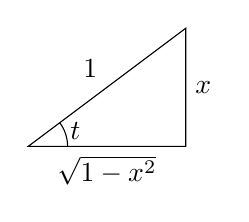
\begin{tikzpicture}
	\draw(0,0)--node[below]{$\sqrt{1-x^{2}}$}(2,0)--node[right]{$x$}(2,1.5)--node[above left]{$1$}cycle;
	\draw(0.5,0)arc(0:36.869897645844:0.5);
	\node at(0.6,0.2){$t$};
\end{tikzpicture}$\qquad$
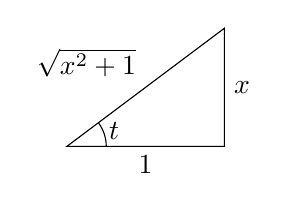
\begin{tikzpicture}
	\draw(0,0)--node[below]{$1$}(2,0)--node[right]{$x$}(2,1.5)--node[above left]{$\sqrt{x^{2}+1}$}cycle;
	\draw(0.5,0)arc(0:36.869897645844:0.5);
	\node at(0.6,0.2){$t$};
\end{tikzpicture}$\qquad$
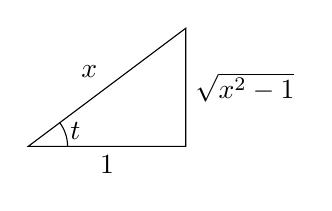
\begin{tikzpicture}
	\draw(0,0)--node[below]{$1$}(2,0)--node[right]{$\sqrt{x^{2}-1}$}(2,1.5)--node[above left]{$x$}cycle;
	\draw(0.5,0)arc(0:36.869897645844:0.5);
	\node at(0.6,0.2){$t$};
\end{tikzpicture}\par
根据这个辅助三角形可以求得$\sin{t}=x,\cos{t}=\sqrt{1-x^{2}},\tan{t}=\frac{x}{\sqrt{1-x^{2}}}$,于是所有用$t$表示的三角函数都可以轻易求得.那么,原式$\frac{1}{2}t+\frac{1}{4}\sin{2t}+C=\frac{1}{2}\arcsin{x}+\frac{1}{2}\sin{t}\cos{t}=\frac{1}{2}\arcsin{x}+\frac{1}{2}x\sqrt{1-x^{2}}$.\par
还有形如$\sqrt{x^{2}+1}$的情形可换元$x=\tan{t},t\in\left(-\frac{\pi}{2},\frac{\pi}{2}\right)$,辅助三角形见上图中;形如$\sqrt{x^{2}-1}$的情形可换元$x=\sec{t},t\in\left[0,\frac{\pi}{2}\right)\bigcup\left(\frac{\pi}{2},\pi\right)$,辅助三角形见上图右.\par
需要特别注意的是,$\sqrt{x^{2}-1}$的换元情形有些特别,因为换元过程中倘若$t\in\left(\frac{\pi}{2},\pi\right)$,就会有$\sqrt{\sec^{2}{t}-1}=\sqrt{\tan^{2}{t}}=-\tan{t}$,这是需要带负号的.\par
除了使用三角换元,还可以使用双曲换元.比如,要消掉根式$\sqrt{x^{2}+1}$,可以令$x=\sinh{t},t\in\mathbb{R}$,于是$\sqrt{x^{2}+1}=\cosh{t}$,就实现了有理化;要消掉根式$\sqrt{x^{2}-1}$,可以分两段考虑:当$x\ge1$时,令$x=\cosh{t},t\in\left[0,+\infty\right)$,于是$\sqrt{x^{2}-1}=\sinh{t}$;当$x\le-1$时,令$x=-\cosh{t},t\in\left[0,+\infty\right)$,于是$\sqrt{x^{2}-1}=\sinh{t}$.\par
可以看出,存在$\sqrt{x^{2}-1}$的情形时无论用三角换元还是双曲换元,都是不容易处理的,因为都需要对$x\in\left(-\infty,-1\right]\bigcup\left[1,+\infty\right)$进行分区间讨论.下面对于积分$\int\sqrt{x^{2}-1}\dif{x}$分别使用三角换元和双曲换元解题.\par
令$x=\sec{t},t\in\left[0,\frac{\pi}{2}\right)\bigcup\left(\frac{\pi}{2},\pi\right)$.当$t\in\left[0,\frac{\pi}{2}\right)$时$\sqrt{x^{2}-1}=\tan{t}$,于是$\int\sqrt{x^{2}-1}\dif{x}=\int\sec{t}\tan^{2}{t}\dif{t}$;当$x\in\left(\frac{\pi}{2},\pi\right)$时$\sqrt{x^{2}-1}=-\tan{t}$,于是$\int\sqrt{x^{2}-1}\dif{x}=-\int\sec{t}\tan^{2}{t}\dif{t}$.积分然后回代即可.\par
当$x\in\left[1,+\infty\right)$时,令$x=\cosh{t},t\in\left[0,+\infty\right)$,于是$\int\sqrt{x^{2}-1}\dif{x}=\int\sinh^{2}{t}\dif{t}$;当$x\in\left(-\infty,-1\right]$时,令$x=-\cosh{t},t\in\left[0,+\infty\right)$,于是$\int\sqrt{x^{2}-1}\dif{x}=-\int\sinh^{2}{t}\dif{t}$.\par
不过一般而言,如果读者对双曲函数和反双曲函数的性质比较陌生,就尽量不要使用双曲换元.这是因为,使用三角换元可以方便地画辅助三角形示意图,但使用双曲换元就很难画辅助双曲线示意图了.因此在回代过程中,三角换元的效率比较高.\par
事实上,所有形如$\sqrt{ax^{2}+bx+c}$的结构都可以通过三角/双曲换元来消根号.比如$\sqrt{x^{2}+a^{2}}\;\left(a>0\right)$就可以换元$x=\tan{t},t\in\left(-\frac{\pi}{2},\frac{\pi}{2}\right)$或者$x=\sinh{t},t\in\mathbb{R}$,而根号内存在一次项的情形可以通过配方解决,比如$\sqrt{-x^{2}+x+1}=\sqrt{\frac{5}{4}-\left(x-\frac{1}{2}\right)^{2}}$,那么换元$x-\frac{1}{2}=\frac{\sqrt{5}}{2}\sin{t}$即可.
\subsection{对勾换元}
存在$\sqrt{x^{2}-1}$的情形时,无论用三角换元还是双曲换元,都不可避免地要进行分区间讨论.能否找到一种参数方程,使其不需要分类讨论也能消根号呢?这是有的.\par
考虑到恒等变换$\left(x+x^{-1}\right)^{2}-4=\left(x-x^{-1}\right)^{2}$,也即$\left(\frac{x+x^{-1}}{2}\right)^{2}-1=\left(\frac{x-x^{-1}}{2}\right)^{2}$,倘若在$\sqrt{x^{2}-1}$中换元$x=\frac{t+t^{-1}}{2}$,那么$\sqrt{x^{2}-1}=\sqrt{\left(\frac{t-t^{-1}}{2}\right)^{2}}$,可以开根号.\par
接下来就考虑$t$的取值范围,从而决定开根号的结果.因为$x\in\left(-\infty,-1\right]\bigcup\left[1,+\infty\right)$,而对勾函数的性质决定了在$t>0$的区间内取$t\in\left(0,1\right]$或者$t\in\left[1,+\infty\right)$都可以满足$x\ge1$;在$t<0$的区间内取$t\in\left(-\infty,-1\right]$或者$t\in\left[-1,0\right)$都可以满足$x\le-1$.那么如何取$t$的范围更好呢?\par
考虑到开根号的问题,当$t\in\left(-\infty,-1\right]\bigcup\left(0,1\right]$时$\sqrt{\left(\frac{t-t^{-1}}{2}\right)^{2}}=\frac{t^{-1}-t}{2}$,而当$t\in\left[-1,0\right)\bigcup\left[1,+\infty\right)$时$\sqrt{\left(\frac{t-t^{-1}}{2}\right)^{2}}=\frac{t-t^{-1}}{2}$,那么为了避免分类讨论开根号的结果,可以限制$t\in\left[-1,0\right)\bigcup\left[1,+\infty\right)$,这样$x$的值域满足了,且开平方的结果无需分类讨论.当然,限制$t\in\left(-\infty,-1\right]\bigcup\left(0,1\right]$也是完全可以的.\par
那么接下来考虑另一个问题,将$x$都换为$t$的有关形式后,如何回代?因为$x=\frac{t+t^{-1}}{2},\sqrt{x^{2}-1}=\frac{t-t^{-1}}{2}$,所以两式相加得$t=x+\sqrt{x^{2}-1}$,作差得$t^{-1}=x-\sqrt{x^{2}-1}$.于是原式中的$t,\frac{1}{t}$都能很容易地进行回代.\par
举例来说,积分$\int\sqrt{x^{2}-1}\dif{x}$中令$x=\frac{t+t^{-1}}{2},t\in\left[-1,0\right)\bigcup\left[1,+\infty\right)$,于是就有$\sqrt{x^{2}-1}=\frac{t-t^{-1}}{2}$.那么原积分化为$\int\frac{t-t^{-1}}{2}\dif{\frac{t+t^{-1}}{2}}=\frac{1}{4}\int\left(t-t^{-1}\right)\left(1-t^{-2}\right)\dif{t}=\frac{1}{8}t^{2}-\frac{1}{2}\ln{|t|}-\frac{1}{8}t^{-2}+C=\frac{1}{2}x\sqrt{x^{2}-1}-\frac{1}{2}\ln{|x+\sqrt{x^{2}-1}|}+C$.\par
\subsection{欧拉换元}
拿到根式$y=\sqrt{ax^{2}+bx+c}\;\left(a\ne0\right)$,可以先判断一下各个参数的范围,然后考虑其在平面直角坐标系上的函数图形.\par
首先,$a<0$时不需要讨论$b^{2}-4ac\le0$,因为此种情形下一定有$ax^{2}+bx+c<0$,于是$\sqrt{ax^{2}+bx+c}$就没有实数定义域;而当$b^{2}-4ac=0$时$\sqrt{ax^{2}+bx+c}$只在一点有实数定义域.\par
将原式化为$y^{2}=ax^{2}+bx+c\Leftrightarrow\left(\sqrt{-a}x-\frac{b}{2\sqrt{-a}}\right)^{2}+y^{2}=\frac{4ac-b^{2}}{4a}\;\left(y\ge0\right)$.可见它是椭圆的一部分(例外的是,当$a=-1$时它是圆的一部分).\par
而当$a>0$时,如果$b^{2}-4ac=0$,直接配方开根号,当作绝对值函数处理即可,那么分两种情形讨论:如果$b^{2}-4ac<0$,那么$y^{2}=ax^{2}+bx+c\Leftrightarrow y^{2}-\left(\sqrt{a}x+\frac{b}{2\sqrt{a}}\right)^{2}=\frac{4ac-b^{2}}{4a}\;\left(y>0\right)$,这是焦点连线平行于$y$轴的双曲线上半部分;如果$b^{2}-4ac>0$,那么$y^{2}=ax^{2}+bx+c\Leftrightarrow\left(\sqrt{a}x+\frac{b}{2\sqrt{a}}\right)^{2}-y^{2}=\frac{b^{2}-4ac}{4a}\;\left(y\ge0\right)$,这是焦点位于$x$轴上双曲线的一部分.\par
由解析几何可以知道,直线和圆锥曲线至多有两个交点.假如在原图像上取一个点$\left(x_{0},\sqrt{ax_{0}^{2}+bx_{0}+c}\right)$作出斜率为$t$的直线方程$y=t\left(x-x_{0}\right)+\sqrt{ax_{0}^{2}+bx_{0}+c}$,那么只要合理限制参数$t$的取值,就可以得到另一个交点,然后列出方程$\sqrt{ax^{2}+bx+c}=t\left(x-x_{0}\right)+\sqrt{ax_{0}^{2}+bx_{0}+c}$并解出$x$与$t$的关系就可以.\par
可以看出,这个方程的形式是特别丑陋的,主要原因是取定点过于随意.如果取一个合适的点,就可以大大简化计算.不妨重新考虑取点产生的直线方程$y=t\left(x-x_{0}\right)+\sqrt{ax_{0}^{2}+bx_{0}+c}$,如果取$x_{0}=0$的话,该方程中所有$x_{0}$都可以直接消掉,从而化简为$y=tx+\sqrt{c}$.这样取的前提是$x=0$处有定义,等价于$c\ge0$.\par
于是,当$c\ge0$时就可以设直线$y=tx+\sqrt{c}$,然后联立方程$\begin{cases}y=\sqrt{ax^{2}+bx+c}\\y=tx+\sqrt{c}\end{cases}$,得$ax^{2}+bx=t^{2}x^{2}+2\sqrt{c}tx$,那么就解出$x_{0}=0,x_{1}=\frac{b-2\sqrt{c}t}{t^{2}-a}$.所以说,在曲线上除了$\left(0,\sqrt{c}\right)$以外的每个点都可以用关于$t$的参数方程$\begin{cases}x=-\frac{b-2\sqrt{c}t}{t^{2}-a}\\y=t\left(\frac{b-2\sqrt{c}t}{t^{2}-a}\right)+\sqrt{c}\end{cases}$的形式来表示,就实现了有理化.这种式子不建议死记,读者在搞懂其中原理之后可以自行推导.\par
如果原根式$\sqrt{ax^{2}+bx+c}$满足$b^{2}-4ac>0$,可以进行因式分解,那么可以考虑取曲线与$x$轴的交点作为定点.设$ax^{2}+bx+c$的两个不等实根分别为$x_{1},x_{2}$,于是因式分解为$\sqrt{a\left(x-x_{1}\right)\left(x-x_{2}\right)}$.在点$\left(x_{1},0\right)$处作斜率为$t$的直线$y=t\left(x-x_{1}\right)$就可以.这样做的前提是函数与$x$轴有交点,等价于$b^{2}-4ac>0$.\par
于是,当$b^{2}-4ac>0$时可以设两实根$x_{1},x_{2}$,于是因式分解为$a\left(x-x_{1}\right)\left(x-x_{2}\right)$.然后联立方程$\begin{cases}y=\sqrt{a\left(x-x_{1}\right)\left(x-x_{2}\right)}\\y=t\left(x-x_{1}\right)\end{cases}$,得$a\left(x-x_{1}\right)\left(x-x_{2}\right)=t^{2}\left(x-x_{1}\right)^{2}$,那么解出$x_{0}=\frac{t^{2}x_{1}-ax_{2}}{t^{2}-a}$.所以说,在曲线上除了$\left(x_{1},0\right)$以外的每个点都可以用关于$t$的参数方程$\begin{cases}x=\frac{t^{2}x_{1}-ax_{2}}{t^{2}-a}\\y=t^{2}\left(\frac{t^{2}x_{1}-ax_{2}}{t^{2}-a}-x_{1}\right)\end{cases}$的形式来表示,就实现了有理化.\par
以上方法是通过取图像上一定点作直线来保证至多只有另外一个交点的.还有一种情况下直线与圆锥曲线只有一个交点,那就是平行于双曲线渐近线的直线.\par
双曲线$y^{2}-\left(\sqrt{a}x+\frac{b}{2\sqrt{a}}\right)^{2}=\frac{4ac-b^{2}}{4a}\;\left(y\ge0\right)$的渐近线为$\pm y=\sqrt{a}x+\frac{b}{2\sqrt{a}}$,这里为简明起见,直接作其中一条渐近线的平行直线$y=\sqrt{a}x+t$,其中$t$是纵截距参数.那么只要限制$t$取合适的值,直线和双曲线就会有且只有一个交点.这样做的前提是原函数图像为双曲线的一部分,即$a>0$.\par
那么联立方程$\begin{cases}y=\sqrt{ax^{2}+bx+c}\\y=\sqrt{a}x+t\end{cases}$,得$x=\frac{t^{2}-c}{b-2\sqrt{a}t}$,于是双曲线上的每个点都可以用关于$t$的参数方程$\begin{cases}x=\frac{t^{2}-c}{b-2\sqrt{a}t}\\y=\frac{\sqrt{a}t^{2}-\sqrt{a}c}{b-2\sqrt{a}t}+t\end{cases}$的形式来表示,就实现了有理化.\par
接下来考虑另一个问题,将原积分转化成关于$t$的有理函数积分后,如何进行回代?其实很简单,因为在换元式中只有一处$t$,显化就相当容易.比如说$y=tx+\sqrt{c}$可显化为$t=\frac{\sqrt{ax^{2}+bx+c}-\sqrt{c}}{x}$;$y=t\left(x-x_{1}\right)$可显化为$t=\frac{\sqrt{ax^{2}+bx+c}}{x-x_{1}}$;$y=\sqrt{a}x+t$可显化为$\sqrt{ax^{2}+bx+c}-\sqrt{a}x$.\par
互相比较一下就不难发现,第三种方法化出来的式子最简单,第二种次之,第一种方法化出来的式子最繁琐.而在实际操作过程中,当然是计算量越小越有利,所以在选择欧拉换元时,尽量用第三种方法,再次用第二种方法,不得已再用第一种方法.\par
可以想到,对于$y=\sqrt{ax^{2}+bx+c}\;\left(a\ne0,b^{2}-4ac\ne0\right)$凡有$a>0$的情况,都可以使用第三种方法,那就用$y=\sqrt{a}x+t$换元即可.那么继续考虑$a<0$的情况,此时若有$b^{2}-4ac<0$,那么$y$在实数域无定义域,那么只考虑$b^{2}-4ac>0$即可.而此时都可以用第二种方法,那就因式分解为$y=\sqrt{a\left(x-x_{1}\right)\left(x-x_{2}\right)}$然后用换元$y=t\left(x-x_{1}\right)$就可以了.那么综上所述,第一种方法没有使用的必要.\par
更严酷的事实是,欧拉换元因为计算量非常大,已经不推荐使用了.既然三角/双曲换元已经能解决这类根式积分问题,欧拉换元就显得没有必要了.相对于简洁、易懂的三角换元来说,欧拉换元从推导到式子变换都有很大可能出错,而偏偏计算和回代又很繁琐,所以如今的不定积分已不再推荐使用欧拉换元解决问题.\par
\section{分式线性替换与切比雪夫定理}
分式线性替换是形如$x=\frac{ct+d}{at+b}\;\left(a\ne0\right)$的换元.可以看出$\frac{ct+d}{at+b}=\frac{c}{a}+\frac{ad-bc}{a^{2}t+ab}$,这是反比例函数经平移变换后得到的形式.这种变换拥有很好的性质,尤其是具有反函数$t=\frac{d-bx}{ax-c}$,于是由$x$换元成$t$以及相应的回代过程都比较容易.\par
本节介绍分式线性替换在切比雪夫定理中的一些应用.\par
\subsection{统一根式的分式线性替换方法}
在介绍幂函数换元的过程中提到,如果被积函数中同时出现两个根式而不容易同时消掉,可以考虑先消掉其中一个根式.比如说$\int\frac{1+\sqrt{x+1}}{1+\sqrt{x}}\dif{x}$中就换元$x=t^{2}$.于是只剩下一个含二次多项式的无理式部分.这也是在原函数难以被化简的情况下最推荐的做法.\par
除此之外,分式线性替换也可以发挥作用.以$\int\frac{1+\sqrt{x+1}}{1+\sqrt{x}}\dif{x}$为例,倘若通过替换$t^{2}=\frac{x+1}{x},t\in\left(1,+\infty\right)\Leftrightarrow x+1=t^{2}x$将$\sqrt{x+1}$全部变为$t\sqrt{x}$,就可以在不引入新根号的前提下,将所有的根式都统一为$\sqrt{x}$了.\par
这里需要补充一点,变换$\sqrt{x+1}=\sqrt{t^{2}x}=\sqrt{t^{2}}\sqrt{x}$过程中的拆根式是有条件的,需要$t^{2}$与$x$都为非负值才可以.而事实上这是不需要担忧的,因为被积函数中含有的偶次根号已经将$x$的值域限制住了.\par
那么再解决变量统一的问题.原式$x+1=t^{2}x$可以变形为$x=\frac{1}{t^{2}-1}$,那么将所有的$x$都用$t$来表示就好,这个过程中依然不会引入新的根式,只不过原来的$\sqrt{x}$会变成$\frac{1}{\sqrt{t^{2}-1}}$,这是化成了根号下二次多项式的形式了.\par
所以整理一下步骤就能够得到$\int\frac{1+\sqrt{x+1}}{1+\sqrt{x}}\dif{x}=\int\frac{1+t\sqrt{x}}{1+\sqrt{x}}\dif{x}=\int\frac{\sqrt{t^{2}-1}+t}{\sqrt{t^{2}-1}+1}\dif{\frac{1}{t^{2}-1}}$.\par
这里使用分式线性替换的目的很简单,就是将根式统一为同种并且不引入新的根式.为了使用分式线性替换,就要用一个简单变量替换$\frac{x+1}{x}$从而通过中间变量实现$\sqrt{x+1}$到$\sqrt{x}$的转化.而为了不引入新的根式,就要保证中间变量开二次方根后依旧是有理的,所以设$t^{2}=\frac{x+1}{x}$是最合适的选择.\par
事实上这种操作非常麻烦,不如直接换元$x=t^{2}$.但要放在这里介绍的目的是引入更为实用的情形,那就是二项式微分的积分.\par
\subsection{简单二项式微分的处理}
形如$x^{m}\left(a+bx^{r}\right)^{n}\dif{x}$的微分式叫做二项式微分,其中$a,b$为任意常数(实际上默认$b\ne0$,因为$b=0$时情况就变得非常简单),$m,n,r$为任意有理数.本小节主要研究相对简单的形式,即$r=1$的情况下,形如$\int x^{m}\left(a+bx\right)^{n}\dif{x}$的积分.\par
假如$m,n$都为整数,这个积分就是有理函数积分.直接按照有理函数积分的方法进行即可.\par
假如$n$为整数而$m$为有理分数,如果将$m$表示为两个整数$p,q$的最简整数比,那么原积分可以写作$\int\sqrt[q]{x^{p}}\left(a+bx\right)^{n}\dif{x}$.这个式子中只有简单的单一根号,那么用换元$x=t^{q}$($t$的取值范围依实际情况而定,下同)就可以消掉根号,化为有理函数积分$q\int t^{p+q-1}\left(a+bt^{q}\right)^{n}\dif{t}$.\par
假如$m$为整数而$n$为有理分数呢,这和上面的例子是同理的,因为可以通过线性换元$u=a+bx$将所有的$x$换元为$u$,于是变成$\frac{1}{b^{m+1}}\int u^{n}\left(u-a\right)^{m}\dif{u}$,其中$m$为整数而$n$为有理分数.那么仿照上一段的操作解决问题即可.\par
而假如$m,n$都为有理分数,情况就会比较复杂.这里仅根据切比雪夫整理的结论加以说明:当且仅当$m+n\in\mathbb{Z}$时,这个二项式微分的积分结果才能够用初等函数表达.\par
这里记整数$k=m+n$,既然如此$m,n$的最简整数比形式一定有着相同的分母$q$.将原积分改写为$\int\sqrt[q]{x^{qm}}\sqrt[q]{\left(a+bx\right)^{qn}}\dif{x}$,其中$q,qm,qn$都是整数.\par
这里出现了两个根式,能否简化为一个根式?可以尝试使用分式线性替换.首先确定中间变量的次数,当然是设为$q$次最稳妥了.于是设$t^{q}=\frac{x}{a+bx}\Leftrightarrow x=t^{q}\left(a+bx\right)$,于是有$\sqrt[q]{x^{qm}}=\sqrt[q]{t^{q^{2}m}\left(a+bx\right)^{qm}}$,那么$\sqrt[q]{x^{qm}}\sqrt[q]{\left(a+bx\right)^{qn}}=\sqrt[q]{t^{q^{2}m}\left(a+bx\right)^{qk}}=t^{qm}\left(a+bx\right)^{k}$.\par
接下来将$x$也用$t$来表达,即通过等式$x=t^{q}\left(a+bx\right)$得到$x=\frac{at^{q}}{1-bt^{q}},a+bx=\frac{a}{1-bt^{q}}$,于是原积分化为$\int t^{qm}\frac{a^{k}}{\left(1-bt^{q}\right)^{k}}\dif{\frac{at^{q}}{1-bt^{q}}}$,这就是关于$t$的有理函数积分了.\par
这里简单考虑一下$t$的取值范围和回代的问题.当$q$为奇数时,这里涉及的所有根式都为奇数次,不用考虑被开方数的正负,$t$的取值范围完全取决于$\frac{x}{a+bx}$的值域,即$t\in\left(-\infty,\frac{1}{b}\right)\bigcup\left(\frac{1}{b},+\infty\right)$,回代时也是直接开奇数次方即可.而当$q$为偶数时,这里涉及的所有根式都为偶数次,那就要保证$x\ge0,a+bx\ge0$,那么显然有$t\ge0$,于是开方就无需考虑被开方数的正负,拆根式也可以直接拆,$t$的定义域显得不那么重要,感兴趣的读者可以自行研究.\par
回代也很方便,直接开方得到$t=\sqrt[q]{\frac{x}{a+bx}}$即可.\par
大量的参数非常恼人,这里举几个例题说明之:\par
积分$\int\sqrt[3]{\frac{x}{x+1}}\dif{x}$也即$\int x^{\frac{1}{3}}\left(x+1\right)^{-\frac{1}{3}}\dif{x}$是满足次数和为整数($0$)的条件的.令$t^{3}=\frac{x}{x+1}$,则有$x=\frac{t^{3}}{1-t^{3}}$,那么原积分化为$\int t\dif{\frac{t^{3}}{1-t^{3}}}$.这里有一个技巧问题,如果直接将微分项中的$\frac{t^{3}}{1-t^{3}}$求导并入被积函数中化为$-\int\frac{3t^{3}}{\left(1-t^{3}\right)^{2}}\dif{t}$,这个式子的形式就会非常丑陋.但倘若通过分部积分法进行操作$\int t\dif{\frac{t^{3}}{1-t^{3}}}=\frac{t^{4}}{1-t^{3}}-\int\frac{t^{3}}{1-t^{3}}\dif{t}$,再进行积分就会简单很多.\par
积分$\int\sqrt[4]{x^{3}}\sqrt[4]{x+1}\dif{x}$是满足次数和为整数($1$)的条件的.令$t^{4}=\frac{x+1}{x}$,则有$x=\frac{1}{t^{4}-1}$,于是原积分化为$\int tx\dif{x}=\int\frac{t}{t^{4}-1}\dif{\frac{1}{t^{4}-1}}$.这里仍然需要观察,如果直接求导并入被积函数,分母降变为12次,这显然是不好办的.但倘若通过凑微分和分部的方式将其简化,就要好处理一些.$\int t\frac{1}{t^{4}-1}\dif{\frac{1}{t^{4}-1}}=\frac{1}{2}\int t\dif{\frac{1}{\left(t^{4}-1\right)^{2}}}=\frac{t}{2\left(t^{4}-1\right)^{2}}-\frac{1}{2}\int\frac{\dif{t}}{\left(t^{4}-1\right)^{2}}$.这样产生的新积分分母为8次,起码比直接求导要方便很多.\par
\subsection{切比雪夫定理}
接下来考虑较为复杂的二项式微分情形,从而引出切比雪夫定理.根据前一小节的内容可以知道,在$\int x^{m}\left(a+bx\right)^{n}\dif{x}$中,只要$m,n,m+n$三者之中有一个为整数,就可以通过幂函数换元或分式线性替换的方法解出这个积分.那么倘若二项式微分$x^{m}\left(a+bx^{r}\right)^{n}\dif{x}$中的$r\ne1$,能否将其化为上一小节中所介绍的类型呢?\par
考虑凑微分$\dif{x}=\frac{1}{r}\cdot\frac{1}{x^{r-1}}\dif{x^{r}}$并换元$u=x^{r}$,这样就能够将$\left(a+bx^{r}\right)^{n}$转换成$\left(a+bu\right)^{n}$的形式.那么接下来将变量统一为$u$就行了.\par
开根号$\sqrt[r]{u}=\sqrt[r]{x^{r}}=x$,这里不需要带绝对值符号,感兴趣的读者可以自行分类讨论验证.于是将$x=\sqrt[r]{u}$代入$\frac{1}{r}\int x^{m}\left(a+bu\right)^{n}\frac{\dif{u}}{x^{r-1}}=\frac{1}{r}\int u^{\frac{m+1-r}{r}}{\left(a+bu\right)^{n}}\dif{u}$\par
可以看出,这样换元就很容易地把问题化成了简单二项式微分的积分.那么根据之前的结论,只要$\frac{m+1}{r},n,\frac{m+1}{r}+n$三者之中有一个为整数,就可以通过幂函数换元或分式线性替换的方法解出这个积分.特别地,当$r=1$时只需要研究$m,n,m+n$即可,这也是上述论述的一个特例.\par
切比雪夫定理就描述了这样一个事实:在积分$\int x^{m}\left(a+bx^{r}\right)^{n}\dif{x}$中,只要$\frac{m+1}{r},n,\frac{m+1}{r}+n$三者之中有一个为整数,这个积分就可以用初等函数来表达.其它情形下二项式微分的积分都是不能用初等函数表达的(狭义上称作“不可积”).这里举几个例题:\par
积分$\int x^{5}\sqrt[3]{x^{3}+1}\dif{x}$可以考虑先凑$\dif{x^{3}}$并换元以简化根号内的式子,所以得到$\int x^{5}\sqrt[3]{x^{3}+1}\dif{x}=\frac{1}{3}\int x^{3}\sqrt[3]{x^{3}+1}\dif{x^{3}}=\frac{1}{3}\int u\sqrt[3]{u+1}\dif{u}\;\left(u=x^{3}\right)$.\par
然后可以换元$u+1=t^{3},t\in\mathbb{R}$,得到$\int\left(t^{6}-t^{3}\right)\dif{t}=\frac{1}{7}t^{7}-\frac{1}{4}t^{4}+C$.接下来回代$t=\sqrt[3]{u+1}=\sqrt[3]{x^{3}+1}$即可.\par
再举一例,积分$\int\sqrt{\left(x^{2}+1\right)^{3}}\dif{x}$的处理.这里可以先考虑$x\ge0$的情况,$x<0$时一律代$-x$计算即可.那么限制$x\ge0$时,考虑凑$\dif{x}=\frac{1}{2x}\dif{x^{2}}$换元$u=x^{2},u\in\left[0,+\infty\right)$,得到$\frac{1}{2}\int\frac{\sqrt{\left(u+1\right)^{3}}}{\sqrt{u}}\dif{u}$.\par
然后可以换元$t^{2}=\frac{u+1}{u},t\in\left(1,+\infty\right)$,将原积分化为$\frac{1}{2}\int t^{3}u\dif{u}=\frac{1}{4}\int t^{3}\dif{u^{2}}=\frac{1}{4}t^{3}u^{2}-\frac{1}{2}\int\frac{3t^{2}\dif{t}}{\left(1-t^{2}\right)^{2}}$,后续按照有理函数积分法解决即可.接下来回代$t=\frac{\sqrt{x^{2}+1}}{x}$即可.\par
当$x<0$时,一律将积分变量凑成$-x$即可代上面的结果.\par
\section{二次根式专题}
含二次根式的积分是无理函数积分中最常见的类型,这类积分的被积函数有各种可以利用的性质.本节主就含二次根式的积分进行研究.\par
需要指出,这里仅研究根号内不超过二次多项式的情形,因为根号内超过二次的积分若无特殊结构,一般是无解的.这里也只讨论被积函数中只含一个二次根式,或者容易化成每个被积函数只含一个二次根式的类型.\par
\subsection{常用公式}
这三个基本公式是可以用三角/双曲换元轻松证明的,这是二次根式积分的基础:\\
$\int\frac{\dif{x}}{\sqrt{1-x^{2}}}=\arcsin{x}+C$\\
$\int\frac{\dif{x}}{\sqrt{x^{2}-1}}=\ln{|x+\sqrt{x^{2}-1}|}+C$\\
$\int\frac{\dif{x}}{\sqrt{x^{2}+1}}=\ln{\left(x+\sqrt{x^{2}+1}\right)}+C$\par
有了这些结论,只需要用正比例换元$x=at\;\left(a>0\right)$就可以轻松得到以下公式:\\
$\int\frac{\dif{x}}{\sqrt{a^{2}-x^{2}}}=\arcsin{\frac{x}{a}}+C$\\
$\int\frac{\dif{x}}{\sqrt{x^{2}-a^{2}}}=\ln{|x+\sqrt{x^{2}-a^{2}}|}+C$\\
$\int\frac{\dif{x}}{\sqrt{x^{2}+a^{2}}}=\ln{\left(x+\sqrt{x^{2}+a^{2}}\right)}+C$\par
当然用三角/双曲换元也是可以一步完成的,比如令$x=a\sin{t}$代入$\int\frac{\dif{x}}{\sqrt{a^{2}-x^{2}}}$中.
对于$\int\frac{\dif{x}}{\sqrt{ax^{2}+bx+c}}\;\left(a\ne0\right)$的情形,可以考虑使用配方法将其变为$\begin{cases}\int\frac{\dif{x}}{\sqrt{\left(\sqrt{a}x+\frac{b}{2\sqrt{a}}\right)^{2}+\frac{4ac-b^{2}}{4a}}}\;\left(a>0\right)\\\int\frac{\dif{x}}{\sqrt{\frac{4ac-b^{2}}{4a}-\left(\sqrt{-a}x-\frac{b}{2\sqrt{-a}}\right)^{2}}}\;\left(a<0\right)\end{cases}$接着通过换元法套上面的公式就可以了.\par
所以整理成通式如下,有需要的读者可以尝试记忆,这能有助于加快计算:\\
记$Y=ax^{2}+bx+c\;\left(a\ne0\right),\Delta=b^{2}-4ac$.\\
当$a>0$时,$\int\frac{\dif{x}}{\sqrt{Y}}=\frac{1}{\sqrt{a}}\ln{\left(Y'+2\sqrt{aY}\right)}+C$;\\
当$a<0$时,$\int\frac{\dif{x}}{\sqrt{Y}}=\frac{1}{\sqrt{-a}}\arcsin{\frac{-Y'}{\sqrt{\Delta}}}+C$\par
\subsection{分母只含根式的情形}
积分$\int\frac{\dif{x}}{\sqrt{ax^{2}+bx+c}}\;\left(a\ne0,\text{下同}\right)$是可以套用第一小节中通式解决的,实际操作中可以根据参数的值采用相对容易的方法.\par
积分$\int\frac{px+q}{\sqrt{ax^{2}+bx+c}}\dif{x}$可以仿照$\int\frac{px+q}{ax^{2}+bx+c}\dif{x}$的方法进行,通过拼凑和分项将其化为两个积分,其中一个分子可凑微分,另一个分子只含常数.\par
例如,积分$\int\frac{x+2}{\sqrt{x^{2}+2x+2}}\dif{x}=\frac{1}{2}\int\frac{2x+2}{\sqrt{x^{2}+2x+2}}\dif{x}+\int\frac{\dif{x}}{\sqrt{\left(x+1\right)^{2}+1}}=\frac{1}{2}\int\frac{\dif{\left(x^{2}+2x\right)}}{\sqrt{x^{2}+2x+2}}+\int\frac{\dif{\left(x+1\right)}}{\sqrt{\left(x+1\right)^{2}+1}}=\sqrt{x^{2}+2x+2}+\ln{\left(x+1+\sqrt{x^{2}+2x+2}\right)}+C$.\par
再考虑更复杂一点的情形,如果分子上有二次乃至更高次的多项式呢?可以使用分部积分法的循环功能来解决.举个最简单的例子:$\int\frac{x^{2}\dif{x}}{\sqrt{x^{2}1}}=\frac{1}{2}\int\frac{x\dif{x^{2}}}{\sqrt{x^{2}+1}}=\int x\dif{\sqrt{x^{2}+1}}=x\sqrt{x^{2}+1}-\int\sqrt{x^{2}+1}\dif{x}=x\sqrt{x^{2}+1}-\int\frac{x^{2}\dif{x}}{\sqrt{x^{2}+1}}-\int\frac{\dif{x}}{\sqrt{x^{2}+1}}$,接下来就是移项操作了,化简后可以得到$\int\frac{x^{2}\dif{x}}{\sqrt{x^{2}+1}}=\frac{1}{2}x\sqrt{x^{2}+1}-\ln{\left(x+\sqrt{x^{2}+1}\right)}$.\par
那么假如分子是三次的呢?就更简单了,直接凑微分$\dif{x^{2}}$就可以了,比如说$\int\frac{x^{3}\dif{x}}{\sqrt{x^{2}+1}}=\frac{1}{2}\int\frac{x^{2}\dif{x^{2}}}{\sqrt{x^{2}+1}}$.\par
而当分母根式中含有一次项时,可以通过配方线性换元将一次项消去,以下举一例:\\
$\int\frac{x^{2}\dif{x}}{\sqrt{x^{2}+2x}}=\int\frac{\left(x+1-1\right)^{2}\dif{\left(x+1\right)}}{\sqrt{\left(x+1\right)^{2}-1}}=\int\frac{u^{2}-2u+1}{\sqrt{u^{2}-1}}\dif{u}\;\left(\text{令}u=x+1\right)=\int\frac{u^{2}}{\sqrt{u^{2}-1}}\dif{u}-\int\frac{\dif{u^{2}}}{\sqrt{u^{2}-1}}+\int\frac{\dif{u}}{\sqrt{u^{2}-1}}$\par
分母为更高次数的情形也是同理,这里不介绍奇数次情形了,主要介绍偶数次情形.比如说$\int\frac{x^{4}\dif{x}}{\sqrt{x^{2}+1}}$,就可以通过多次分部积分的方法逐步降低次数,这也是分部积分法去幂作用的一个体现.\\
$\int\frac{x^{4}\dif{x}}{\sqrt{x^{2}+1}}=\int x^{3}\dif{\sqrt{x^{2}+1}}=x^{3}\sqrt{x^{2}+1}-3\int x^{2}\sqrt{x^{2}+1}\dif{x}=x^{3}\sqrt{x^{2}+1}-3\int\frac{x^{4}\dif{x}}{\sqrt{x^{2}+1}}-3\int\frac{x^{2}\dif{x}}{\sqrt{x^{2}+1}}\Rightarrow\int\frac{x^{4}\dif{x}}{\sqrt{x^{2}+1}}=\frac{1}{4}x^{3}\sqrt{x^{2}+1}-\frac{3}{4}\int\frac{x^{2}\dif{x}}{\sqrt{x^{2}+1}}$\par
综合本小节内容来看,倘若分母只有一个二次根式(且根式内只有一个二次多项式),无论分子是何种情况,总能够通过适当的方法解出这个积分.\par
\subsection{分母为根式与一次多项式之积的情形}
分母为根式与一次多项式之积时,这类积分常用倒代换方法解决.最经典的例子是$\int\frac{\dif{x}}{x\sqrt{x^{2}+1}}=\int\frac{\dif{x}}{x\left|x\right|\sqrt{x^{-2}+1}}=\sgn{x}\int\frac{\dif{x}}{x^{2}\sqrt{x^{-2}+1}}=-\sgn{x}\int\frac{\dif{x^{-1}}}{\sqrt{x^{-2}+1}}=-\ln{\left(x^{-1}+\sqrt{x^{-2}+1}\right)}\sgn{x}+C$.\par
这里需要注意将$x^{2}$提出根式时开方要带绝对值或者处理成符号函数.按理说将原函数写成这个形式就可以了,但这里既有符号函数又有$x^{-1}$,看上去比较丑陋,可以将它化为更简洁的形式.这里需要分类讨论一下.\par
当$x\ge0$时,原函数写作$-\ln{\left(\frac{1}{x}+\frac{\sqrt{x^{2}+1}}{x}\right)}+C=\ln{\frac{x\left(\sqrt{x^{2}+1}-1\right)}{\left(\sqrt{x^{2}+1}+1\right)\left(\sqrt{x^{2}+1}-1\right)}}+C=\ln{\frac{\sqrt{x^{2}+1}-1}{x}}+C$;而当$x<0$时,原函数则写作$\ln{\left(\frac{1}{x}-\frac{\sqrt{x^{2}+1}}{x}\right)}+C=\ln{\frac{\sqrt{x^{2}+1}-1}{-x}}+C$.化到这里就可以出结论了:$\int\frac{\dif{x}}{x\sqrt{x^{2}+1}}=\ln{\frac{\sqrt{x^{2}+1}-1}{\left|x\right|}}+C$.\par
再举一例,$\int\frac{\dif{x}}{\left(x+1\right)\sqrt{x^{2}+1}}$就需要使用换元$x+1=\frac{1}{t}$,那么这个积分化为$\int\frac{t\dif{\frac{1}{t}}}{\sqrt{\frac{1}{t^{2}}-\frac{2}{t}+2}}=-\sgn{t}\int\frac{\dif{t}}{\sqrt{2t^{2}-2t+1}}$,这样就变成了分母只含二次根式的积分了.\par
分母有一次多项式重因式的情形依然可以通过倒代换来解决,比如说$\int\frac{\dif{x}}{x^{2}\sqrt{x^{2}+1}}=\sgn{x}\int\frac{\dif{x}}{x^{3}\sqrt{x^{-2}+1}}=-\frac{\sgn{x}}{2}\int\frac{\dif{x^{-2}}}{\sqrt{x^{-2}+1}}=-\sgn{x}\sqrt{x^{-2}+1}+C=-\frac{\sqrt{x^{2}+1}}{x}+C$,再如$\int\frac{\dif{x}}{x^{3}\sqrt{x^{2}+1}}=-\int\frac{\dif{x^{-1}}}{x\sqrt{x^{2}+1}}=-\sgn{x}\int\frac{x^{-2}\dif{x^{-1}}}{\sqrt{x^{-2}+1}}$,这便是上一小节中提及的需要使用分部积分法的类型了.\par
\subsection{根号移分母原则}
在解决二次根式积分时常常会遇到形如$\int\frac{\sqrt{x^{2}+1}}{x}\dif{x}$这样的积分.拿到这道题,倘若不用三角换元,简化这个被积函数就很难了.这里的困难主要体现在以下几个方面:\par
\begin{enumerate}
	\item 前面介绍过的积分很多可以通过在分子中拼凑项的方法构成可以与分母约分的形式.但本题不同,无论分子如何拼凑,都无法改变被积函数中的$\frac{x^{2}+1}{x}$这一项,约分成无稽之谈.
	\item 基本积分表的积分都是根式在分母上的,像$\int\frac{\dif{x}}{\sqrt{1-x^{2}}},\int\frac{\dif{x}}{\sqrt{x^{2}\pm1}}$.根式在分子上的情形没有对应的基本积分表,无法套用基本积分公式直接解出.
\end{enumerate}
要解决这种困难,方法就是将根号放到分母.这是通过恒等变换实现的,就本例而言,做法是$\int\frac{\sqrt{x^{2}+1}}{x}\dif{x}=\int\frac{x^{2}+1}{x\sqrt{x^{2}+1}}\dif{x}$接下来,分子变成了整多项式,可以通过分项、拼凑的方法构造容易解出的积分类型.在本例中,直接分项为$\int\frac{x}{\sqrt{x^{2}+1}}\dif{x}+\int\frac{\dif{x}}{x\sqrt{x^{2}+1}}$即可,这里产生的两个新积分就是前面讨论过的类型了.\par
对比一下这三个积分$\int\sqrt{\frac{1-x}{1+x}}\dif{x},\int\frac{\sqrt{1-x^{2}}}{1+x}\dif{x},\int\frac{1-x}{\sqrt{1-x^{2}}}\dif{x}$,它们的被积函数其实是完全一样的,但显然第一个和第二个比较难处理.第一个还可以使用分式线性替换,第二个却只能靠三角换元了.但倘若通过恒等变换将根号放到分母上,变成第三个的形式,这就成了非常容易解决的积分了.\\
$\int\frac{1-x}{\sqrt{1-x^{2}}}\dif{x}=\int\frac{\dif{x}}{\sqrt{1-x^{2}}}-\int\frac{x\dif{x}}{\sqrt{1-x^{2}}}=\arcsin{x}+\sqrt{1-x^{2}}+C$\par
总之,遇到分子上的二次根式,优先考虑通过恒等变换挪到分母上,再拼凑分子来简化被积函数,往往会容易得多.\par
另有一种将根号移到分母的方案就是分部积分法,这是因为$\frac{\dif}{\dif{x}}\sqrt{ax^{2}+bx+c}=\frac{2ax+b}{2\sqrt{ax^{2}+bx+c}}$.倘若被积函数中除根式以外的因子很容易凑微分,那就将根式单独放到被积函数中,其它部分凑微分,分部积分就可以将根号放在分母上了.\\
$\int\frac{\sqrt{1-x^{2}}}{x^{2}}\dif{x}=-\int\sqrt{1-x^{2}}\dif{\frac{1}{x}}=-\frac{\sqrt{1-x^{2}}}{x}-\int\frac{1}{\sqrt{1-x^{2}}}\dif{x}=-\frac{\sqrt{1-x^{2}}}{x}-\arcsin{x}+C$\par
不过这种方法并不常用,因为事实上直接恒等变换将根号放分母就足够简便了.过程为$\int\frac{\sqrt{1-x^{2}}}{x^{2}}\dif{x}=\int\frac{1}{x^{2}\sqrt{1-x^{2}}}\dif{x}-\int\frac{\dif{x}}{\sqrt{1-x^{2}}}$,其后不难.\par
\subsection{平方差公式化简被积函数}
前面的小节讨论过了被积函数分母只含一个根式,或者是一个根式乘一些多项式因子的形式.倘若分母不止有一个根式,问题处理起来就会麻烦很多.举例来说,积分$\int\frac{1}{\sqrt{x^{2}+x+1}+x}\dif{x}$的分母含有根式与多项式的和.分母上的多项式无法裂项,这种形式会让初学者无从下手,这时候就需要使用分母有理化的方法来解决分母上的问题了.\par
使用平方差公式,将原本的积分变形为$\int\frac{\sqrt{x^{2}+x+1}-x}{x+1}\dif{x}$.这样将分母变形为一个常规多项式,而分子的形式可以直接裂项.其中$\int\frac{x}{x+1}\dif{x}$是一个有理函数积分,那么只需要集中精力解决$\int\frac{\sqrt{x^{2}+x+1}}{x+1}\dif{x}$就可以了.\par
这个新积分的难点在于根号位于分子,那么按照上一小节的思路,通过恒等变换将其挪到分母上,变为$\int\frac{x^{2}+x+1}{\left(x+1\right)\sqrt{x^{2}+x+1}}\dif{x}$.\par
接下来处理这个积分,可以分项将其变为$\int\frac{x}{\sqrt{x^{2}+x+1}}\dif{x}+\int\frac{\dif{x}}{\left(x+1\right)\sqrt{x^{2}+x+1}}$.对于第一项,解法是拼凑$\int\frac{x+\frac{1}{2}}{\sqrt{x^{2}+x+1}}\dif{x}-\frac{1}{2}\int\frac{\dif{x}}{\sqrt{x^{2}+x+1}}$,而第二项直接倒代换$x+1=\frac{1}{t}$就可以解决问题.\par
合理地使用平方差公式能够将分母有理化,有效简化运算.举一个经典的例子,积分$\int\frac{\dif{x}}{\sqrt{x+1}+\sqrt{x}}=\int\frac{\sqrt{x+1}-\sqrt{x}}{x+1-x}\dif{x}=\frac{2}{3}\sqrt{x+1}^{3}-\frac{2}{3}\sqrt{x}^{3}+C$.\par
这种化简是很有效的,只是适用范围比较有限.\par
\subsection{阿贝尔换元的简单应用}
先来介绍一个重要公式:$\int\frac{\dif{x}}{\sqrt{ax^{2}+b}^{3}}\;\left(a,b\ne0\right)=\frac{x}{b\sqrt{ax^{2}+b}}+C$.这个公式的证明可以通过求导验证,积分方法可以选择切比雪夫定理的应用.\par
这个原函数还可以写作$\frac{1}{b}\sqrt{\frac{x^{2}}{ax^{2}+b}}+C$,可以看出,这样的变换把所有的$x$项都处理为$x^{2}$项,倘若有一个被积函数$R\left(x^{2}\right)$是关于$x^{2}$的有理式,那么积分$\int\frac{R\left(x^{2}\right)}{\sqrt{ax^{2}+b}^{3}}\dif{x}=\frac{1}{b}\int R\left(x^{2}\right)\dif{\frac{x}{\sqrt{ax^{2}+b}}}=\frac{\sgn{x}}{b}\int R\left(x^{2}\right)\dif{\sqrt{\frac{x^{2}}{ax^{2}+b}}}$.这个变换的意义在于,原本的积分中还有单独的$x$在微分项中,而变换之后只剩下关于$x^{2}$的形式了.\par
接下来考虑另外一个问题,被积函数中所有的$x^{2}$都可以使用关于$\frac{x^{2}}{ax^{2}+b}$的函数表示出来.这里$\frac{\frac{ax^{2}}{ax^{2}+b}}{1-\frac{ax^{2}}{ax^{2}+b}}=\frac{ax^{2}}{b}\Leftrightarrow x^{2}=\frac{b}{a}\cdot\frac{\frac{ax^{2}}{ax^{2}+b}}{1-\frac{ax^{2}}{ax^{2}+b}}$.这里令$u=\sqrt{\frac{x^{2}}{ax^{2}+b}}$,那么$x^{2}=\frac{bu^{2}}{1-au^{2}}$.\par
总结上述内容,最开始的积分可以逐步化成$\frac{1}{b}\int R\left(\frac{bu^{2}}{1-au^{2}}\right)\dif{u}$,这是关于$u$的有理函数积分,于是乎问题就可以得到解决了.\par
接下来举一些经典的例子:\\
$\int\frac{\dif{x}}{\sqrt{x^{2}-1}^{5}}=-\int\frac{1}{x^{2}-1}\dif{\frac{x}{\sqrt{x^{2}-1}}}=-\sgn{x}\int\left(\frac{x^{2}}{x^{2}-1}-1\right)\dif{\sqrt{\frac{x^{2}}{x^{2}-1}}}=-\frac{2}{3}\sqrt{\frac{x^{2}}{x^{2}-1}}^{3}\sgn{x}+\sqrt{\frac{x^{2}}{x^{2}-1}}\sgn{x}+C=-\frac{2x^{3}}{3\sqrt{x^{2}-1}^{3}}+\frac{x}{\sqrt{x^{2}-1}}+C$\\
$\int\frac{\dif{x}}{\sqrt{x^{2}+1}^{7}}=-\int\frac{1}{\left(x^{2}+1\right)^{2}}\dif{\frac{x}{\sqrt{x^{2}+1}}}=-\sgn{x}\int\left(1-\sqrt{\frac{x^{2}}{x^{2}+1}}^{2}\right)^{2}\dif{\sqrt{\frac{x^{2}}{x^{2}+1}}}$\\
$\int\frac{x^{2}\dif{x}}{\sqrt{x^{2}+1}^{3}}=\sgn{x}\int x^{2}\dif{\sqrt{\frac{x^{2}}{x^{2}+1}}}=\sgn{x}\int\frac{u^{2}}{1-u^{2}}\dif{u}\;\left(\text{令}u=\sqrt{\frac{x^{2}}{x^{2}+1}}\right)$\par
本题还有另一种解法,是$\int\frac{x^{2}\dif{x}}{\sqrt{x^{2}+1}^{3}}=\frac{1}{2}\int\frac{x\dif{x^{2}}}{\sqrt{x^{2}+1}^{3}}=-\frac{1}{4}\int x\dif{\frac{1}{\sqrt{x^{2}+1}}}=-\frac{x}{4\sqrt{x^{2}+1}}+\frac{1}{4}\int\frac{\dif{x}}{\sqrt{x^{2}+1}}$,这也是一种不错的选择.\\
$\int\frac{1}{\left(x^{2}+2\right)\sqrt{x^{2}+1}}\dif{x}=\int\frac{x^{2}+1}{x^{2}+2}\cdot\frac{\dif{x}}{\sqrt{x^{2}+1}^{3}}=\int\frac{1}{\frac{x^{2}+2}{x^{2}+1}}\dif{\frac{x}{\sqrt{x^{2}+1}}}=\sgn{x}\int\frac{1}{2-\frac{x^{2}}{x^{2}+1}}\dif{\sqrt{\frac{x^{2}}{x^{2}+1}}}$\par
阿贝尔换元可以较简便地解决形如$\int\frac{\dif{x}}{\sqrt{ax^{2}+b}^{2n+1}},\int\frac{\dif{x}}{\sqrt{ax^{2}+b}\left(cx^{2}+d\right)}$的情形,这在上面的例题中都有所体现.\par
再来考虑略微复杂一点的情形.积分$\int\frac{\dif{x}}{\sqrt{ax^{2}+bx+c}^{2n+1}}\;\left(a\ne0\right)$要使用阿贝尔换元并不是什么难事,只要配方成$\int\frac{\dif{x}}{\sqrt{a\left(x+\frac{b}{2a}\right)^{2}+\frac{4ac-b^{2}}{4a}}}$就可以了.这又是形如$\int\frac{\dif{x}}{\sqrt{ax^{2}+b}^{2n+1}}$的形式.\par
但假如说原积分是形如$\int\frac{\dif{x}}{\left(x^{2}+ax+b\right)\sqrt{x^{2}+cx+d}}$的形式,单纯的配方只有在$a=c$时才有作用,否则就无法让这个积分不含$x$项.这类情形要么使用三角换元将其转变为三角函数有理式的积分,要么就使用分式线性替换同时消掉两个式子的一次项.\par
\subsection{分式线性替换方法}
现在有两个二次多项式$x^{2}+ax+b,\,x^{2}+cx+d$,其中$a\ne c$\par.这里使用分式线性替换$x=\frac{At+B}{t+1}$同时消除二者的一次项.\par
考虑到这种方法较为抽象,这里用一个实例来解释它.对于积分$\int\frac{\dif{x}}{\left(x^{2}+2x+2\right)\sqrt{x^{2}+4x+2}}$而言,这里换元$x=\frac{At+B}{t+1}$,其中$A,B$为待定系数.于是$x^{2}+2x+2=\frac{\left(A^{2}+2A+2\right)t^{2}+\left(2AB+2A+2B+4\right)t+\left(B^{2}+2B+2\right)}{\left(t+1\right)^{2}}$.不难想到,这个式子中分母上的$\left(x+1\right)^{2}$在被积函数中会被乘到分子上,而分子无论多么复杂,处理起来都比处理分母要轻松些,所以只需要关注真正处在被积函数分母上的部分即可.\par
在表达式$\left(A^{2}+2A+2\right)t^{2}+\left(2AB+2A+2B+4\right)t+\left(B^{2}+2B+2\right)$中,只需要按照原定目的消去一次项即可,所以列方程$2AB+2\left(A+B\right)+4=0$,得到第一个方程.\par
接下来按照相同的思路考虑$x^{2}+4x+2$.因为已经换元$x=\frac{At+B}{t+1}$,所以$x^{2}+4x+2=\frac{\left(A^{2}+4A+2\right)t^{2}+\left(2AB+4A+4B+4\right)t+\left(B^{2}+4B+2\right)}{\left(t+1\right)^{2}}$.\par
那么同样的道理,令$2AB+4\left(A+B\right)+4=0$即可.于是在这里可以列方程组$\begin{cases}2AB+2\left(A+B\right)=-4\\2AB+4\left(A+B\right)=-4\end{cases}$,解得$\begin{cases}AB=-2\\A+B=0\end{cases}$.于是就用一个方程$x^{2}-2=0$来解出$A=\sqrt{2},B=-\sqrt{2}$(反过来也行)即可.\par
综上所述,设$x=\frac{\sqrt{2}t-\sqrt{2}}{t+1}$,将原积分化为$\sgn{\left(t+1\right)}\int\frac{\left(t+1\right)^{3}}{\left[\left(4+2\sqrt{2}\right)t^{2}+\left(4-2\sqrt{2}\right)\right]\sqrt{\left(4+4\sqrt{2}\right)t^{2}+\left(4-4\sqrt{2}\right)}}\dif{\frac{\sqrt{2}t-\sqrt{2}}{t+1}}$,这样就成功消掉了一次项.\par
最后,分情况处理,分子展开为$t^{3}+3t^{2}+3t+1$,对于分子为奇数次的情形,凑微分$\dif{x^{2}}$处理;对于分子为偶数次的情形,使用阿贝尔换元.\par
笔者认为,用这种分式线性替换的方法解题是一种相当麻烦的解法,并没有比三角换元简便多少.但{\fontencoding{OT2}\selectfont G. M. }菲赫金哥尔茨在他的著作《微积分学教程》中使用这种方法来讲解这类积分的处理方法.依笔者看,之所以使用这种方法,更多地是强调解题的通用性,即这一类的积分都可以用这种方法来解决.然而通用的方法往往也是最复杂的方法,就好比对$\int\frac{\sin{x}}{1+\cos{x}}\dif{x}$使用万能公式法.这种方法的泛用性高,但非常复杂.\par
但实际解决问题时未必如此,人力计算往往只是处理具体的问题,而具体的问题往往可以根据具体的数据情况,找到比通用方法更为便捷的操作.
最后来解决这样一个问题.高次多项式$P\left(x\right),Q\left(x\right)$构成一个无理函数积分$\int\frac{P\left(x\right)}{Q\left(x\right)\sqrt{ax^{2}+bx+c}}\dif{x}\;\left(a\ne0\right)$,如何解决?\par
其实不难,只需要将$\frac{1}{\sqrt{ax^{2}+bx+c}}$视为公因式,将这里的有理函数因子$\frac{P\left(x\right)}{Q\left(x\right)}$裂项即可,这样裂项后的分母一定是二次以内的多项式,再将公因式乘入每一项即可.所以说分母高次多项式因子的情形都可以通过裂项简化为二次及以下的情形,这一类积分都是可以解决的.\par
接下来会补充介绍由 \underline{魏念辉}提出的另一种方法,可供读者学习.\par
\subsection{补充介绍:魏氏方法}
以积分$\int\frac{x-1}{\left(x^{2}+x+1\right)\sqrt{x^{2}+3x+1}}\dif{x}$为例,这里倘若对分子分母同除$x^{\frac{3}{2}}$,就可以化为$\int\frac{x^{-\frac{1}{2}}-x^{-\frac{3}{2}}}{\left(x+x^{-1}+1\right)\sqrt{x+x^{-1}+3}}\dif{x}$.这里凑微分$2\int\frac{\dif{\left(x^{\frac{1}{2}}+x^{-\frac{1}{2}}\right)}}{\left(x+x^{-1}+1\right)\sqrt{x+x^{-1}+3}}$然后对分母变形得到$2\int\frac{\dif{\left(x^{\frac{1}{2}}+x^{-\frac{1}{2}}\right)}}{\left[\left(x^{\frac{1}{2}}+x^{-\frac{1}{2}}\right)^{2}-1\right]\sqrt{\left(x^{\frac{1}{2}}+x^{-\frac{1}{2}}+1\right)}}$这里换元$u=x^{\frac{1}{2}}+x^{-\frac{1}{2}}$,可以发现原积分化为$\int\frac{\dif{u}}{\left(u^{2}-1\right)\sqrt{u^{2}+1}}$,这是使用阿贝尔换元就能解决的类型.\par
再考虑积分$\int\frac{x+1}{\left(x^{2}+x+1\right)\sqrt{x^{2}+3x+1}}\dif{x}$,这里仿照前面的方法操作即可,于是变成$\int\frac{x^{-\frac{1}{2}}+x^{-\frac{3}{2}}}{\left(x+x^{-1}+1\right)\sqrt{x+x^{-1}+3}}\dif{x}=2\int\frac{\dif{\left(x^{\frac{1}{2}}-x^{-\frac{1}{2}}\right)}}{\left[\left(x^{\frac{1}{2}}-x^{-\frac{1}{2}}\right)^{2}+3\right]\sqrt{\left(x^{\frac{1}{2}}-x^{-\frac{1}{2}}\right)^{2}+5}}$.这里再换元$u=x^{\frac{1}{2}}-x^{-\frac{1}{2}}$即可化为$2\int\frac{\dif{u}}{\left(u^{2}+3\right)\sqrt{u^{2}+5}}$,这也是用阿贝尔换元就能解决的类型.\par
既然$\int\frac{x-1}{\left(x^{2}+x+1\right)\sqrt{x^{2}+3x+1}}\dif{x},\int\frac{x+1}{\left(x^{2}+x+1\right)\sqrt{x^{2}+3x+1}}\dif{x}$二者都是可解的,那么以它们作为积木,就可以求出任意一个形如$\int\frac{ax+b}{\left(x^{2}+x+1\right)\sqrt{x^{2}+3x+1}}\dif{x}$的积分来.\par
接下来考虑稍微复杂一点的情形,积分$\int\frac{x\dif{x}}{\left(x^{2}+ax+c\right)\sqrt{x^{2}+bx+c}}\;\left(a\ne b,\,c>0\right)$如何解决?可以仿照上面的思路先处理这个积分,得到$\int\frac{x^{-\frac{1}{2}}\dif{x}}{\left(x+cx^{-1}+a\right)\sqrt{x+cx^{-1}+b}}$.那么应该想方设法化为\\$\int\frac{x^{-\frac{1}{2}}-\sqrt{c}x^{-\frac{3}{2}}}{\left[\left(x^{\frac{1}{2}}+\sqrt{c}x^{-\frac{1}{2}}\right)^{2}+a-2\right]\sqrt{\left(x^{\frac{1}{2}}+x^{-\frac{1}{2}}\right)^{2}+b-2}}\dif{x}$和$\int\frac{x^{-\frac{1}{2}}+\sqrt{c}x^{-\frac{3}{2}}}{\left[\left(x^{\frac{1}{2}}-\sqrt{c}x^{-\frac{1}{2}}\right)^{2}+a+2\right]\sqrt{\left(x^{\frac{1}{2}}-x^{-\frac{1}{2}}\right)^{2}+b+2}}\dif{x}$.这显然也是要依赖积木法进行的.\par
上面只考虑了$c>0$的情形,那么当$c\le0$时会如何呢?很显然在这种条件下一定有$a^{2}-4c\ge0$,那么表达式$x^{2}+ax+c$就存在实根了.如果是重根,那就倒代换;如果不是重根,那就裂项再倒代换.总之就不需要使用分式线性换元或者魏氏方法来处理了,于是这里只需要研究$c>0$的情形就足够.\par
上面讨论的情形是基于两个二次多项式的二次项都为$1$且常数项都为$c$的情形.这里假定将二次项系数统一为$1$,那么假如两个常数项不相同,该如何处理呢?这里选择线性换元,从几何意义上解释这种处理方法.\par
考虑两个二次函数$x^{2}+ax+c,x^{2}+bx+c\;\left(a\ne b\right)$的特征,它们有唯一交点,并且这个交点就位于$y$轴上.而对于两个二次函数$x^{2}+ax+c,x^{2}+bx+d\;\left(c\ne d\right)$来说,它们只有一个交点,但不在$y$轴上.那么只要通过线性换元$x=t+A$,其中$A$是待定系数,就可以将这个交点平移到$tOy$坐标系的$y$轴上,于是就可以使用上述方法了.\par
举例来说,两个二次函数图像$x^{2}+2x+3$与$x^{2}+4x+1$的交点在$x=1$处,那么就令$x=t+1$,于是这两个二次函数图像分别化为$t^{2}+4t+6$和$t^{2}+6t+6$,这样就简单了.\par
接下来举一个全面使用魏氏方法解题的例子,积分$\int\frac{\dif{x}}{\left(x^{2}+4\right)\sqrt{x^{2}+x+1}}$
.在这里令$x=t+3$,那么原积分化为$\int\frac{\dif{t}}{\left(t^{2}+6t+13\right)\sqrt{t^{2}+7t+13}}$.这里使用积木$\int\frac{t^{-\frac{1}{2}}-\sqrt{13}t^{-\frac{3}{2}}}{\left[\left(t^{\frac{1}{2}}+\sqrt{13}t^{-\frac{1}{2}}\right)^{2}+6-2\sqrt{13}\right]\sqrt{\left(t^{\frac{1}{2}}+\sqrt{13}t^{-\frac{1}{2}}\right)^{2}+7-2\sqrt{13}}}\dif{t}$和$\int\frac{t^{-\frac{1}{2}}+\sqrt{13}t^{-\frac{3}{2}}}{\left[\left(t^{\frac{1}{2}}-\sqrt{13}t^{-\frac{1}{2}}\right)^{2}+6+2\sqrt{13}\right]\sqrt{\left(t^{\frac{1}{2}}-\sqrt{13}t^{-\frac{1}{2}}\right)^{2}+7+2\sqrt{13}}}\dif{t}$就可以了.\par
\end{document}